\documentclass[a4paper,UKenglish]{lipics}
\usepackage{mathtools}
\usepackage{stackengine}
\newcommand\letvdash[1]{\mathrel{
  \stackengine{1.2ex}{\vdash}{\;\;\scriptscriptstyle#1}{O}{c}{F}{T}{L}}}
\stackMath

\usepackage{upgreek}%alpha symbol
\usepackage{adjmulticol}
\usepackage[utf8]{inputenc}

\usepackage{xspace}
\usepackage{comment}
\usepackage{multicol}
\usepackage{wasysym}
\usepackage{float}
\usepackage{array}
\usepackage{framed}
\usepackage{amsmath}
\usepackage{amssymb}
\usepackage{stmaryrd}

\usepackage{listings}
\usepackage{algorithm2e}

\usepackage{tikz}
\usepackage{pgfplots}
\usepackage{mathrsfs}
\usepgfplotslibrary{external}
\usetikzlibrary{external}
\tikzexternalize[prefix=tikz/]

\usepackage[
breaklinks=true,colorlinks=true,
%linkcolor=blue,urlcolor=blue,citecolor=blue,% PDF VIEW
linkcolor=black,urlcolor=black,citecolor=black,% PRINT
bookmarks=true,bookmarksopenlevel=2]{hyperref}

% Proof trees
\usepackage{ebproof}


%%% Local Variables:
%%% mode: latex
%%% TeX-master: t
%%% End:

\newcommand*\bang[1]{! #1}
%\newcommand{\ifthenelse}[3]{\texttt{if}\; #1 \texttt{ then}\; #2 \texttt{ else}\; #3}
\newcommand{\match}[4]{\texttt{match}\; #1\; \{ 0 \mapsto #2;\; s(#3) \mapsto #4 \}}

\newcommand{\outputch}[4]{\overline{#1}\langle #2\rangle^{#3}\!.#4}
\newcommand{\inputch}[4]{#1(#2)^{#3}.#4}

\newcommand{\asyncoutputch}[3]{\overline{#1}\!\langle #2\rangle^{#3}}
\newcommand{\asyncinputch}[3]{#1\!\left( #2\right)^{#3}}
\newcommand{\asyncrepinputch}[3]{\bang{\asyncinputch{#1}{#2}{#3}}}


\newcommand{\splitatcommas}[1]{%
  \begingroup
  \begingroup\lccode`~=`, \lowercase{\endgroup
    \edef~{\mathchar\the\mathcode`, \penalty0 \noexpand\hspace{0pt plus 1em}}%
  }\mathcode`,="8000 #1%
  \endgroup
}



\newcommand{\parcomp}[2]{#1 \mid #2}
\newcommand{\parcompthree}[3]{\parcomp{\parcomp{#1}{#2}}{#3}}
\newcommand{\parcompfour}[4]{\parcompthree{#1}{#2}{\parcomp{#3}{#4}}}
\newcommand{\parcompseven}[7]{#1 \mid #2 \mid #3 \mid #4 \mid #5 \mid #6 \mid #7}

\newcommand{\uparcomp}[2]{\parcomp{#1}{#2}}
\newcommand{\uparcompthree}[3]{\uparcomp{\uparcomp{#1}{#2}}{#3}}
\newcommand{\uparcompfour}[4]{\uparcompthree{#1}{#2}{\uparcomp{#3}{#4}}}
\newcommand{\uparcompfive}[5]{\uparcompfour{#1}{#2}{#3}{\uparcomp{#4}{#5}}}

\newcommand{\newvar}[2]{(\nu #1) #2}
\newcommand{\newvarU}[1]{\left(\nu #1\right)}

\newcommand{\nil}{\mathbf{0}}

\newcommand{\freemodule}[0]{\mathbb{Z}[i_1,\dots,i_n]}

\newcommand{\true}{\textit{true}}
\newcommand{\false}{\textit{false}}

\newcommand{\succeeds}{\mathbf{c}}

\newcommand{\succc}[1]{s(#1)}

\newcommand{\tick}[1]{\texttt{tick}.#1}


\newcommand{\dasfwr}[1]{[#1]^{-1}_R}


\newcommand{\subst}[2]{#1\!\left[#2\right]}

\newcommand{\substi}[2]{\{#1/#2\}}

% Type stuff
\newcommand{\withusage}[2]{#1/#2}
\newcommand{\withtype}[2]{#1:#2}
\newcommand{\channeltype}[1]{\texttt{ch}(#1)}
\newcommand{\channeltypeusage}[2]{\withusage{\channeltype{#1}}{#2}}
\newcommand{\inchanneltypeS}[2]{\texttt{in}_{#1}(#2)}
\newcommand{\outchanneltypeS}[2]{\texttt{out}_{#1}(#2)}
\newcommand{\channeltypeS}[2]{\texttt{ch}_{#1}(#2)}
\newcommand{\tparcomp}[2]{\parcomp{#1}{#2}}
\newcommand{\withdelay}[2]{\uparrow^{#1}\!\!#2}
\newcommand{\usagepref}[3]{#1^{#2}_{#3}}
\newcommand{\inusagesym}[0]{\texttt{In}}
\newcommand{\outusagesym}[0]{\texttt{Out}}
\newcommand{\inusagepref}[2]{\usagepref{\inusagesym}{#1}{#2}}
\newcommand{\outusagepref}[2]{\usagepref{\outusagesym}{#1}{#2}}
\newcommand{\repinusagepref}[2]{\bang{\usagepref{\inusagesym}{#1}{#2}}}
\newcommand{\usagerep}[1]{\;*\!#1}
\newcommand{\errres}[0]{\textbf{\texttt{err}}}
\newcommand{\comlabel}[0]{\textbf{com}}

\newcommand{\withcomplex}[2]{#1 \triangleleft #2}

\newcommand{\typenat}[0]{\texttt{Nat}}
\newcommand{\typechanusage}[2]{\withusage{\channeltype{#1}}{#2}}
\newcommand{\kinterval}[2]{\left[#1,#2\right]}
\newcommand{\kintervalsingle}[1]{\left[#1\right]}
\newcommand{\natinterval}[2]{\typenat\!\kinterval{#1}{#2}}
\newcommand{\natintervalsingle}[1]{\typenat\!\left[#1\right]}

\newcommand{\encoding}[1]{\left[\!\left[#1\right]\!\right]}


\newcommand\defeq{\stackrel{\mathclap{\normalfont\tiny\mbox{def}}}{=}}


\newcommand{\servt}[5]{\forall_{#1} #2.\texttt{serv}^{#3}_{#4}(#5)}
\newcommand{\chant}[3]{\texttt{ch}^{#1}_{#2}(#3)}

\newcommand{\servU}[4]{\withusage{\forall #1.\texttt{serv}^{#2}(#3)}{#4}}

\newcommand{\reliableU}[1]{#1\;\text{reliable}\;}
\newcommand{\reliableT}[1]{#1\;\text{reliable}\;}

%\newcommand{\susume}[4]{\langle #1 \rangle^{#2;#3}_{#4}} % old
\newcommand{\susume}[4]{\downarrow^{#2;#3}_{#4}\!\!(#1)} % new
\newcommand{\susumesim}[2]{\downarrow_{#2}\!\!#1}
\newcommand{\tforward}[4]{\susume{#1}{#2}{#3}{#4}}
\newcommand{\tforwardsim}[2]{\susumesim{#1}{#2}}

\newcommand{\vect}[1]{\texttt{(#1)}}
\newcommand{\evect}[2][]{\vect{#2}_{\!#1}}
\newcommand{\cvect}[2][\varphi]{\vect{#2}_{\!#1}}

\newcommand{\normlinearindex}[3][\mathcal{E}(I)]{#2 + \sum_{\alpha\in #1} #3_\alpha i_\alpha}

\newcommand{\monus}[0]{\dot -}
\newcommand{\monusE}[1][\varphi;\Phi]{\monus_{#1}}

% Fede mængder

\newcommand{\skat}[1]{\textbf{#1}\xspace}
\newcommand{\EnvV}{\skat{EnvV}}
\newcommand{\Var}{\skat{Var}}
\newcommand{\Store}{\skat{Store}}
\newcommand{\Loc}{\skat{Loc}}

% De hele tal

\newcommand{\Z}{\ensuremath{\mathbb{Z}}}

% Inferensregler

\newcommand{\condinfrule}[3]
          {\parbox{5.5cm}{$$ {\frac{#1}{#2}}{\qquad
            #3} \hfill  $$}}

\newcommand{\infrule}[2]
          {\parbox{4.5cm}{$$ \frac{#1}{#2}\hspace{.5cm}$$}}

% Regelnavne
           
\newcommand{\runa}[1]{\mbox{\textsc{\protect{(#1})}}}
\newcommand{\runatt}[2]{$[{\mbox{\textsc{#1}}}_{\mbox{\textsc{\small
        #2}}}]$\xspace}

% Pile

\newcommand{\ra}[1][\relax]{\ensuremath \rightarrow_{#1}}
\newcommand{\lra}{\longrightarrow}
\newcommand{\Ra}{\Rightarrow}
\newcommand{\pra}{\ensuremath \rightharpoonup }

% Kantede parenteser

\newcommand{\lag}{\langle}
\newcommand{\rag}{\rangle}
\newcommand{\conf}[1]{\ensuremath{\lag #1 \rag}}

% Mængder

\newcommand{\setof}[2]{\ensuremath{\{ #1 \mid #2 \}}}
\newcommand{\set}[1]{\ensuremath{\{ #1 \}}}

% Kommandoer i Bims

\newcommand{\skib}{\texttt{skip}}
%\newcommand{\ifthenelse}[3]{\texttt{if}\; #1 \; \texttt{then}\; #2 \;
%  \texttt{else}\; #3}
%\newcommand{\whiledo}[2]{\texttt{while}\; #1 \; \texttt{do}\; #2}

% Neu commands
\newcommand{\hole}{(\!\mid\mid\!)}
\newcommand{\nehole}[1]{\mathord{(\!\mid\!\!#1\!\!\mid\!)}}
\newcommand{\prerep}{[^{m}\!\!\//_{\!\!D}]}
\newcommand{\replace}[1]{\lbrbrak #1 \rbrbrak}
\newcommand{\cursor}[1]{\mathord{
    \lBrack\mspace{1mu}#1\mspace{1mu}\rBrack
}}
\newcommand{\breakpoint}[1]{
\mathord{
    \lAngle\mspace{1mu}#1\mspace{1mu}\rAngle
}}
\newcommand{\wellformed}[1]{\letvdash{wf}#1}
\newcommand{\complete}[1]{\letvdash{c}#1}
\newcommand{\cursorexc}[1]{\letvdash{ce}#1}
\newcommand{\nodevalid}[1]{\letvdash{nv}#1}
\newcommand{\cursorctx}[1]{C\!\left[#1\right]}
\newcommand{\cursorctxhole}{\left[\cdot\right]}
\newcommand{\recursion}[2]{#1\!\left(#2\right)}
% Next

\newcommand{\nexte}{\textrm{next}\xspace}

\newcommand{\editelig}[1]{\mathcal{E}#1}
\newcommand{\noteditelig}[1]{\overline{\mathcal{E}#1}}

\newcommand{\consistent}[2]{#1 \sim #2}

% Omvendt \vdash
\usepackage{graphicx}

\makeatletter
\providecommand*{\dashv}{%
  \mathrel{%
    \mathpalette\@dashv\vdash
  }%
}
\newcommand*{\@dashv}[2]{%
  \reflectbox{$\m@th#1#2$}%
}

\newcommand{\f}{\mkern-2mu f\mkern-3mu}%fix f i mathmode

\newcommand{\cmdchild}[1]{\texttt{child}\; #1}
\newcommand{\cmdparent}{\texttt{parent}}
\newcommand{\cmdlambda}[1]{\texttt{lambda}\; #1}
\newcommand{\cmdhole}{\texttt{hole}}
\newcommand{\cmdrec}[1]{\texttt{rec}\; #1.}
\newcommand{\cmdapp}{\texttt{app}}
\newcommand{\cmdbreak}{\texttt{break}}


\newcommand{\condexp}[2]{#1 \Rightarrow #2}
\newcommand{\condexpto}[3]{#1 \Rightarrow #2 \vert #3}

\definecolor{codegreen}{rgb}{0,0.6,0}
\definecolor{codegray}{rgb}{0.5,0.5,0.5}
\definecolor{codepurple}{rgb}{0.58,0,0.82}
\definecolor{backcolour}{rgb}{0.95,0.95,0.92}

\lstdefinestyle{mystyle}{
    backgroundcolor=\color{backcolour},   
    commentstyle=\color{codegreen},
    keywordstyle=\color{magenta},
    numberstyle=\tiny\color{codegray},
    stringstyle=\color{codepurple},
    basicstyle=\ttfamily\footnotesize,
    breakatwhitespace=false,         
    breaklines=true,                 
    captionpos=b,                    
    keepspaces=true,                 
    numbers=left,                    
    numbersep=5pt,                  
    showspaces=false,                
    showstringspaces=false,
    showtabs=false,                  
    tabsize=2
}

\lstset{style=mystyle}

\makeatother

\title{Implementations of Sized Types for Parallel Complexity of
  Message-passing Processes}
\author[1]{Thomas Herrmann}
\author[1,2]{Hans Hüttel}
\author[3]{Naoki Kobayashi}
\author[1]{Mikkel Korup Lauridsen}
\affil[1]{Aalborg University \\
  Aalborg, Denmark}
\affil[2]{University of Copenhagen\\
  Copenhagen, Denmark}
\affil[3]{Tokyo University\\
  Tokyo, Japan}
\authorrunning{T. Herrmann, H. Hüttel, N. Kobayashi and M.K. Lauridsen}

\begin{document}
\maketitle

\begin{abstract}
  We provide a sound framework for analyzing the parallel complexity
  of $\pi$-calculus processes in the form of a type checker and a type
  inference algorithm. The type checker can verify complexity analyses
  of some polynomial- and linear time primitive recursive functions,
  encoded as replicated channel inputs (servers), by using integer
  programming to bound channel synchronizations. The type inference
  algorithm involves over-approximating the constraint satisfaction
  problems; we provide a Haskell implementation using the Z3 SMT
  solver.
\end{abstract}

\thispagestyle{empty}

\section{Introduction}\label{ch:introduction}

Static analysis of computational complexity has long been a central part of algorithm design and computer science as a whole. One way of performing such a static analysis on a program is by means of type-based techniques. Traditionally, soundness properties have pertained to the absence of certain run-time errors, i.e. \textit{well-typed programs do not go wrong} \cite{Milner1978} but  with the advent of behavioral type disciplines, soundness properties that for instance ensure bounds on the resource use of programs have been proved. % If combined with an implementation, i.e. an algorithm that specifies how the rules of a type system are to be used, we may either verify that a specified type based complexity analysis of a program is correct (type-checking), or automate the complexity analysis and infer a complexity bound for a program, if it can be bounded by the type system (type inference).

Research on type systems for computational complexity has originally focused on sequential programs, using a notion of types that can express sizes of terms in a program, referred to as sized types, which have been both formalized and implemented \cite{HofmannAndJost2003,HofmannAndHoffmann2010,HoffmannEtAl2012,LagoGaboardi2012,AvanziniLago2017}. However, there is particularly interest in static complexity analysis of parallel and concurrent computation, following the trend for programs to increase in size, as distributed systems scale better. Moreover, parallel and especially concurrent computation is significantly more difficult to analyze, and so the work on type systems for static complexity analysis has been extended to parallel computation \cite{HoffmannShao2015}, and more recently to the more intricate domain of message-passing processes, using behavioral type disciplines to bound message-passing \cite{BaillotGhyselen2021,BaillotEtAl2021}.

Baillot and Ghyselen \cite{BaillotGhyselen2021} introduce a type system for parallel computational complexity of $\pi$-calculus processes, extended with naturals and pattern matching as a computational model, combining sized types and input/output types to bound synchronizations on channels, and thereby bound the parallel time complexity of a process. Baillot et al. \cite{BaillotEtAl2021} generalize the type system using the more expressive behavioral type discipline usage types \cite{Kobayashi1998,KobayashiEtAl2000}. However, these type systems are quite abstract and build on a notion of sized types that has yet to be implemented in the context of message-passing, and so neither type checking nor type inference has until now been realized for either type system.

In this thesis, we explore the challenges of implementing type checking and type inference for the type system by Baillot and Ghyselen \cite{BaillotGhyselen2021}. An important part of this type system is the concept of indices. That is, arithmetic expressions that may contain index variables that represent unknown sizes, thereby enabling a notion of size polymorphism. Indices appear in sized types, to for instance express the timesteps at which a channel must synchronize, which may depend on the size of a value received on a replicated input. To compute an upper bound on the parallel complexity, a partial order on channel synchronizations is required, represented as index comparisons that we refer to as constraint judgements and read as: \textit{Provided a set of constraints on valuations of index variables, is one index always less than or equal to another?} Many of the challenges that arise for both type checking and type inference are related to either verification or satisfaction of such judgements.%Finally, the type system relies on on a special form of minus that can never give negative results, which breaks many useful mathematical properties.\\

We implement a type checker for the type system by Baillot and Ghyselen. This effort is two-fold: We define algorithmic type rules and show how constraint judgements on linear indices can be verified using integer programming or alternatively be over-approximated as linear programs. The type system makes heavy use of subtyping, which we partially account for using \textit{combined complexities} that are effectively sets of indices with a number of associated functions that enable us to discard indices we can guarantee to be bounded by other indices. Combined complexities have the advantage that we can defer finding a single index representing a least upper bound until a later time, and we can in fact show that the combined complexity of a closed process can always be reduced to a singleton, i.e. a singular complexity bound.

We prove that our type checker is sound with regards to time complexity, and to this effort we prove a subject reduction property. Our soundness results guarantee that the bounds assigned to well-typed processes by our type checker are indeed upper bounds on the parallel complexity. To increase the expressiveness of the type checker, we also show how constraints on monotonic univariate polynomial indices can be reduced to linear constraints.

We also define a type inference algorithm for the type system by Baillot and Ghyselen. We take a constraint based approach akin to that of \cite{HofmannAndJost2003,HofmannAndHoffmann2010,HoffmannEtAl2012,KobayashiEtAl2000,Kobayashi2005,Lhoussaine2004}, where unknown indices are represented by \textit{templates}: linear functions over a set of known index variables with unknown coefficients represented by coefficient variables. Inspired by  Kobayashi et al. \cite{KobayashiEtAl2000}, we first infer simple types, which are then used to infer a constraint satisfaction problem on use-capabilities and subtyping which we then reduce to constraints of the form $\exists\alpha_1,\dots,\alpha_n.\forall i_1,\dots,i_m.C_1\land\cdots\land C_k \implies I \leq J$ where $\alpha_1,\dots,\alpha_n$ are coefficient variables, $i_1,\dots,i_m$ are index variables, $C_1,\dots,C_k$ are inequality constraints on indices and $I$ and $J$ are indices.

We provide a Haskell implementation of our type inference algorithm using the Z3 SMT solver \cite{Z3}. We naively eliminate universal quantifiers by over-approximating our constraints using coefficient-wise inequality constraints. We account for antecedents $C_1,\dots,C_k$ by substitution. For instance, if we can deduce that coefficient $c$ is positive in the constraint $\exists\alpha_1,\dots,\alpha_n.\forall i_1,\dots,i_j,\dots,i_m.K \leq L + ci_j \land C_1 \land \cdots \land C_k \implies I \leq J$, then we can simulate the antecedent by substituting $\frac{K-L}{c} + i_j$ for $i_j$, i.e. $\exists\alpha_1,\dots,\alpha_n.\forall i_1,\dots,i_j,\dots,i_m.C_1\{\frac{K-L}{c} + i_j/i_j\} \land \cdots \land C_k\{\frac{K-L}{c} + i_j/i_j\} \implies I\{\frac{K-L}{c} + i_j/i_j\} \leq J\{\frac{K-L}{c} + i_j/i_j\}$. Using these over-approximations, our implementation is able to infer precise bounds on several processes containing replicated inputs with linear time complexity.


%%% Local Variables:
%%% mode: latex
%%% TeX-master: "../esop2023"
%%% End:

\input{sections/picalculus}
\section{Sized types for parallel complexity}

In this section, we introduce the type system for parallel complexity of message-passing processes introduced in Baillot and Ghyselen \cite{BaillotGhyselen2021}. This type system builds on the foundations of indices and constraint judgements and formalizes parallel complexity analysis of $\pi$-calculus processes. Due to extensive use of subtyping and the challenges involved in verifying and satisfying constraint judgements, substantial modifications must be made to enable type checking and type inference of processes. 

The type system for parallel complexity of message-passing processes introduced by Baillot and Ghyselen uses sized types to express parametric complexity of replicated input invocation, and thereby achieves precise bounds on primitively recursive processes: A class of processes behaving as primitively recursive functions. This requires a notion of polymorphism in the message types of replicated inputs. Baillot and Ghyselen introduce size polymorphism by bounding sizes of algebraic terms and synchronizations on channels with indices that may contain index variables representing unknown sizes. We may interpret an index with an index valuation that maps its index variables to naturals, such that the index may be evaluated to a natural number.

We first formally define indices and constraints on the valuations of indices. We give both a predicate logic and a model-theoretic interpretation of judgements on such constraints, referring to these as \textit{constraint judgements}. We then define sized types, the subtyping relation and introduce non-algorithmic type rules.

\subsection{Indices and constraint judgements}\label{sec:indicesandjudgements}
In the type system by Baillot and Ghyselen, indices are used to keep track of sizes of inputs received on replicated inputs. As these sizes may be parametric, in that they may be dependent on the sizes of values received on replicated inputs, we view indices as algebraic expressions consisting of index variables $i,j,k\in\mathcal{V}$ ranging over a countable set, and function symbols, using meta-variable $f$, that may represent natural number constants as nullary functions as well as algebraic operators
\begin{align*}
    I,J ::= i \mid f(I_1,I_2,\dots,I_n)
\end{align*}
Each function symbol $f$ has an arity $\text{ar}(f)$ and an interpretation $[\![f]\!] : \mathbb{N}^{\text{ar}(f)} \rightarrow \mathbb{N}$. For the interpretation of binary difference, we assume that $[\![-]\!](n,m) = 0$ when $m \geq n$, which we refer to as the \textit{monus} operator. As indices may contain index variables, we assume some index valuation $\rho : \mathcal{V} \rightarrow \mathbb{N}$, and extend the definition of interpretations to indices, such that $[\![I]\!]_\rho$ is a natural number instance of index $I$, according to index valuation $\rho$, where for all $i$ in $I$, $\rho(i)$ substitutes for $i$ denoted $I\{\rho(i)/i\}$. Index substitution is defined in Definition \ref{def:indexsubstitution}. Based on the structure of the process that indices are used in the typing of, we may be able to establish relationships between the instances of these indices. For instance, a replicated input may receive values of sizes defined by an interval of two indices $[I,J]$. Then, we are only interested in index valuations $\rho$ that satisfy $[\![I]\!]_\rho \leq [\![J]\!]_\rho$. To express such relationships, we define binary constraints on indices in Definition \ref{def:indexconstr}.

\begin{definition}\label{def:indexsubstitution}
    We define index substitution by the following rules
    \begin{align*}
        i\substi{I}{j} &= j \text{ if } i = j\\
        i\substi{I}{j} &= i \text{ if } i \not = j\\
        f(I_1, I_2, \dots, I_n)\substi{J}{i} &= f(I_1\substi{J}{i}, I_2\substi{J}{i}, \dots, I_n\substi{J}{i})
    \end{align*}
\end{definition}

\begin{definition}[Index constraints]\label{def:indexconstr}
    Given a finite set of index variables $\varphi\subset \mathcal{V}$, we define a constraint $C$ on $\varphi$ to be an expression of the form $I \bowtie J$, where $I$ and $J$ are indices with all free index variables in $\varphi$ and $\bowtie\;\in\{\leq,=,\geq\}$ is a binary relation on $\mathbb{N}$. A finite set of constraints is represented by meta-variable $\Phi$.
\end{definition}
%
A constraint $I \bowtie J$ on $\varphi$ is satisfied given an index valuation $\rho : \varphi \longrightarrow \mathbb{N}$ when $[\![I]\!]_\rho \bowtie [\![J]\!]_\rho$ is satisfied, denoted $\rho \vDash I \bowtie J$. For a finite set of constraints $\Phi$, we write $\rho\vDash \Phi$ when $\rho \vDash C$ holds for all $C \in \Phi$. Finally, $\varphi;\Phi\vDash C$ holds when for all index valuations $\rho$ such that $\rho\vDash \Phi$ holds, we also have $\rho\vDash C$. That is, $\varphi;\Phi\vDash C$ holds exactly when $C$ does not impose further restrictions on index valuations on $\varphi$. Such judgements are fundamental to the type system by Baillot and Ghyselen, especially ones of the form $\varphi;\Phi\vDash I \leq J$, as they impose a partial order on indices wrt. how indices may be interpreted. This enables a notion of subtyping for parametric complexities, such that only indices that are greater or equal may substitute, thus preserving upper bounds on the global parallel complexity, as we shall see in the following sections.

\subsection{Alternative formulations of constraint judgements}\label{sec:cjalternativeform}

There are several equivalent formulations of the problem of verifying the judgement $\varphi;\Phi\vDash C_0$. One such formulation is that the judgement holds, when the conjunction of constraints in $\Phi$ implies $C_0$, i.e. assuming that $n \bowtie m$ evaluates to a truth value based on membership in the relation $\bowtie$, the predicate formula $C_1 \land \cdots \land C_n \implies C_0$, where $\Phi = \{C_1,\dots,C_n\}$, must be satisfied for all valuations $\rho$ over $\varphi$. That is, let $C_i = I_i \bowtie_i J_i$, then for any valuation $\rho : \varphi \rightarrow \mathbb{N}$, the formula $([\![I_1]\!]_\rho \bowtie_1 [\![J_1]\!]_\rho) \land \cdots \land ([\![I_n]\!]_\rho \bowtie_n [\![J_n]\!]_\rho) \implies [\![I_0]\!]_\rho \bowtie_0 [\![J_0]\!]_\rho$ must be satisfied. Another interpretation of the problem is that the intersection of the feasible regions of all (inequality) constraints in $\Phi$ must be contained in the feasible region of $C_0$, or equivalently, the set of all valuations over $\varphi$ that satisfy all the constraints in $\Phi$, referred to as the model space of $\Phi$ wrt. $\varphi$, $\mathcal{M}_\varphi(\Phi)$ must be a subset of the model space of $C_0$ wrt. $\varphi$ \begin{equation*}
    \mathcal{M}_\varphi(\Phi) \subseteq \mathcal{M}_\varphi(\{C_0\})\quad\text{where}\quad\mathcal{M}_\varphi(\Phi)=\{\rho : \varphi \rightarrow \mathbb{N} \mid \rho \vDash C\;\text{for}\; C \in \Phi\}
\end{equation*}
or equivalently
\begin{equation*}
    \forall \rho \in \mathcal{M}_\varphi(\Phi) (\rho \in \mathcal{M}_\varphi(\{C_0\}))
\end{equation*}

Finally, given the fact that the current statement of the problem is expressed using a universal quantifier, we can negate the problem, obtaining a problem that can instead be expressed using an existential quantifier by the fact that $\neg \forall x P(x)$ is equivalent to $\exists x \neg P(x)$. This means the problem can also be expressed as 
%
\begin{equation*}
    \neg (\exists \rho \in \mathcal{M}_\varphi(\Phi) (\rho \not\in \mathcal{M}_\varphi(\{C_0\})))
\end{equation*}
or equivalently
\begin{equation*}
    \mathcal{M}_\varphi(\Phi) \cap \mathcal{M}_\varphi'(\{C_0\}) = \emptyset \quad\text{where}\quad
    \begin{matrix}
        \mathcal{M}_\varphi(\Phi)=\{\rho : \varphi \rightarrow \mathbb{N} \mid \rho \vDash C\;\text{for all}\; C \in \Phi\}\\
        \mathcal{M'}_\varphi(\Phi)=\{\rho : \varphi \rightarrow \mathbb{N} \mid \rho \not\vDash C\;\text{for some}\; C \in \Phi\}
    \end{matrix}
\end{equation*}
Notice that $\mathcal{M}_\varphi'(\{C\})$ is equivalent to $\mathcal{M}_\varphi(\{C'\})$ where $C'$ is the inverse constraint of constraint $C$, and so $\mathcal{M}_\varphi(\Phi) \cap \mathcal{M}_\varphi'(\{C_0\}$) = $\mathcal{M}_\varphi(\Phi \cup \{C_0'\})$ given some method to invert constraints. Thus, the problem can also be expressed simply as
\begin{equation*}
    \mathcal{M}_\varphi(\Phi \cup \{C_0'\}) = \emptyset \quad \text{where } C_0' = \text{inverse of } C_0
\end{equation*}

In Example \ref{exmp:judgementsatisfaction}, we show how a judgement can be verified manually using the predicate logic and model-theoretic interpretations of judgements provided above.
%
\begin{example}\label{exmp:judgementsatisfaction}
    Given index variables $\varphi = \{i, j, k\}$ and constraints $\Phi = \{C_1, C_2, C_3, C_4\}$ where
    \begin{align*}
        C_1 &= i \geq 4\\
        C_2 &= j \geq 2\\
        C_3 &= -k + 3 < 0\\ % k \leq 4
        C_4 &= i + j + k \leq 11
    \end{align*}
    we want to check if $\varphi; \Phi \vDash 2i + j^2 + 3k \geq 20$ always holds. %For this example we assume interpretations are as expected from usual mathematical notation.\\
    Namely, we are interested in verifying whether the constraint $2i + j^2 + 3k \geq 20$ imposes any additional constraints to the index variables $i$, $j$ and $k$ given the existing constraints $C_1$, $C_2$, $C_3$ and $C_4$. In this case, we can notice that the minimum values of $i$, $j$ and $k$ are $4$, $2$ and $4$ respectively. As such, given these constraints, the minimum value $2i + j^2 + 3k$ may evaluate to is $2 \cdot 4 + 2^2 + 3 \cdot 4 = 24$. As such, we can conclude that $\varphi; \Phi \vDash 2i + j^2 + 3k \geq 20$ always holds.\\
    
    We can also consider the predicate logic interpretation of the example. It suffices to only consider the index valuations that satisfy the conjunction of constraints, of which there are four. Here, we represent a valuation $\rho$ as a set of pairs of the form $\{(i,\rho(i)) \mid i\in\varphi\}$, and so we have $\{(i,4),(j,2),(k,4)\}$, $\{(i,5),(j,2),(k,4)\}$, $\{(i,4),(j,3),(k,4)\}$ and $\{(i,4),(j,2),(k,5)\}$. We can then verify the corresponding implications to show that the judgement holds
    %
    \begin{align*}
        (4 \geq 4) \land (2 \geq 2) \land ({-4}+3 < 0) \implies 4+2+4 \leq 11\\
        %
        (5 \geq 4) \land (2 \geq 2) \land ({-4}+3 < 0) \implies 5+2+4 \leq 11\\
        %
        (4 \geq 4) \land (3 \geq 2) \land ({-4}+3 < 0) \implies 4+3+4 \leq 11\\
        %
        (4 \geq 4) \land (2 \geq 2) \land ({-5}+3 < 0) \implies 4+2+5 \leq 11
    \end{align*}
    Or correspondingly in model-theoretic notation
    {\small
    \begin{align*}
        \mathcal{M}_\varphi(\Phi) =&\; \{\{(i,4),(j,2),(k,4)\}, \{(i,5),(j,2),(k,4)\}, \{(i,4),(j,3),(k,4)\}, \{(i,4),(j,2),(k,5)\}\}\\
        \mathcal{M}_\varphi(\{2i+j^2+3k\geq 20\}) =&\; \{\{(i,n_1),(j,n_2),(k,n_3)\} \mid n_1,n_2,n_3\in\mathbb{N},\; 2n_1 + n_2^2 + 3n_3 \geq 20 \}\\
        \mathcal{M}_\varphi(\Phi) \subseteq&\; \mathcal{M}_\varphi(\{2i+j^2+3k\geq 20\})
    \end{align*}}
    % \begin{align*}
    %     \mathcal{M}_\varphi(\Phi) = \left\{\{(i,4),(j,2),(k,4)\}, \{(i,5),(j,2),(k,4)\}, \{(i,4),(j,3),(k,4)\}, \{(i,4),(j,2),(k,5)\}\right\}
    % \end{align*}
    
    We can also solve the inverse of the mode-theoretic interpretation of the problem. Then we want to show that $\mathcal{M}_\varphi(\Phi) \cap \mathcal{M}_\varphi'(\{2i+j^2+3k\geq 20\}) = \emptyset$ or equivalently $\mathcal{M}_\varphi(\Phi \cup \{2i+j^2+3k < 20\}) = \emptyset$. 
    %
    \begin{align*}
        \mathcal{M}_\varphi(\{2i+j^2+3k < 20\}) =&\; \{\{(i,n_1),(j,n_2),(k,n_3)\} \mid n_1,n_2,n_3\in\mathbb{N},\; 2n_1 + n_2^2 + 3n_3 < 20 \}\\
        &\kern-9em\mathcal{M}_\varphi(\Phi) \cap \mathcal{M}_\varphi'(\{2i+j^2+3k\geq 20\}) = \mathcal{M}_\varphi(\Phi \cup \{2i+j^2+3k < 20\}) = \emptyset
    \end{align*}
  \end{example}
  
\subsection{Types and subtyping}\label{sec:typesandsubs}

We now introduce the types from the type system of Baillot and Ghyselen. The types include a base type describing naturals as algebraic terms with sizes bounded by an interval consisting of two indices. This enables us to statically reason about how sizes of data structures change throughout reduction of processes, providing us termination guarantees for some forms of recursion. The type system of Baillot and Ghyselen contains lists as an additional base type, however for conciseness of the type system, we only consider naturals.
%
\begin{align*}
    T,S ::=&\; \texttt{Nat}[I,J] \mid \texttt{ch}_I^\sigma(\widetilde{T}) \mid \forall_I\widetilde{i}.\texttt{serv}_K^\sigma(\widetilde{T})
\end{align*}
%
We use input/output types for channels, and we further distinguish between channels that have replicated inputs, i.e. channels that have recursive behavior, and those that do not. We refer to the former as \textit{servers}, and we more specifically require all inputs on such channels to be replicated for technical convenience. Both servers and normal channels are annotated with an index $I$ that for a normal channel represents the number of time steps remaining before the channel synchronizes, and for a server the remaining time before it becomes available. Note that this imposes a temporal linearity constraint onto normal channels, as such channels can synchronize at exactly one time step. For servers we have an additional index $K$ that represents the parametric complexity of invoking the continuation of a replicated input on the server. Finally, the set $\sigma \subseteq \{\texttt{in},\texttt{out}\}$ is a subset of use-capabilities. Since types consist partly of indices, we define index substitution on types in Definition \ref{def:typeindexsubstitution}.\\

\begin{definition}\label{def:typeindexsubstitution}
    We define index substitution on types by the following rules
    \begin{align*}
        \natinterval{I}{J}\substi{K}{i} &= \natinterval{I\substi{K}{i}}{J\substi{K}{i}}\\
        \chant{\sigma}{I}{\widetilde{T}}\substi{J}{i} &= \chant{\sigma}{I\substi{J}{i}}{\widetilde{T}\substi{J}{i}}\\
        \servt{I}{\widetilde{i}}{\sigma}{K}{\widetilde{T}}\substi{J}{j} &= \servt{I\substi{J}{j}}{\widetilde{i}}{\sigma}{K}{\widetilde{T}} \text{ if } j \in \widetilde{i}\\
        \servt{I}{\widetilde{i}}{\sigma}{K}{\widetilde{T}}\substi{J}{j} &= \servt{I\substi{J}{j}}{\widetilde{i}}{\sigma}{K\substi{J}{j}}{\widetilde{T}\substi{J}{j}} \text{ if } j \not\in \widetilde{i}
    \end{align*}
\end{definition}


Subtyping for base types and types is the least reflexive relation $\sqsubseteq$ that satisfies the subtyping rules in Table \ref{tab:subtypeSized}. As the type system should provide upper bounds on the parallel complexity of processes, it is safe to weaken the bounds on the sizes of natural types. That is, we may decrease the lower bound and increase the upper bound on the sizes of such terms. For server and channel types, we may relax use-capabilities and use the subtyping relation on parameter types as well as modify the complexity bounds on servers, depending on the use-capabilities. Servers and channels of input/output capability are invariant, those of input capability are covariant and those of output capability are contravariant. That is, if a server or channel that inputs a value of type $T$ is required, then we can safely use a server or channel that inputs a subtype of $T$, respectively. Conversely, when a server or channel of output capability is required, we can safely use a channel or server that outputs a supertype of the required parameter type \cite{PierceSangiorgi1996}. This becomes apparent when we assume types $\texttt{Integer}$ and $\texttt{Real}$ such that $\texttt{Integer} \sqsubseteq \texttt{Real}$, as any process that receives reals can also safely receive integers, and any process that output reals can also safely output integers. Unlike Baillot and Ghyselen \cite{BaillotGhyselen2021}, we do not discard associations from our type contexts, rather we discard use-capabilities from channels and servers. Thus, to ensure the type checker is sound, we introduce rules $\runa{BGS-cempty}$ and $\runa{BGS-sempty}$ such that channel and server types are super types of ones with no use-capabilities.

%
\begin{table*}[h!]
    \begin{framed}\vspace{-1em}\begin{align*}
        &\kern0em\runa{BGS-nweak}\;\infrule{\varphi;\Phi\vDash I' \leq I\quad\quad \varphi;\Phi\vDash J \leq J'}{
        \varphi;\Phi\vdash \texttt{Nat}[I,J] \sqsubseteq \texttt{Nat}[I',J']}
        %
        \kern3em\runa{BGS-cinvar}\;\infrule{\varphi;\Phi\vdash \widetilde{T}\sqsubseteq\widetilde{S}\quad\quad \varphi;\Phi\vdash \widetilde{S}\sqsubseteq\widetilde{T}}{\varphi;\Phi\vdash\texttt{ch}_I^{\{\texttt{in},\texttt{out}\}}(\widetilde{T}) \sqsubseteq \texttt{ch}_I^{\{\texttt{in},\texttt{out}\}}(\widetilde{S})}\kern7em\\[-1em]
        %
        \vspace{-0.5em}
        &\kern-0em\runa{BGS-ccovar}\;\infrule{\{\texttt{in}\}\subseteq\sigma\quad\varphi;\Phi\vdash \widetilde{T}\sqsubseteq\widetilde{S}}{\varphi;\Phi\vdash \texttt{ch}_I^{\sigma}(\widetilde{T})\sqsubseteq\texttt{ch}_I^{\{\texttt{in}\}}(\widetilde{S})}\quad\quad\runa{BGS-ccontra}\;\infrule{\{\texttt{out}\}\subseteq\sigma\quad\varphi;\Phi\vdash \widetilde{S}\sqsubseteq\widetilde{T}}{\varphi;\Phi\vdash \texttt{ch}_I^{\sigma}(\widetilde{T})\sqsubseteq \texttt{ch}_I^{\{\texttt{out}\}}(\widetilde{S})}\\[-1em]
        %
        &\kern4em\runa{BGS-sinvar}\;\infrule{(\varphi,\widetilde{i});\Phi\vdash \widetilde{T}\sqsubseteq\widetilde{S}\quad\quad (\varphi,\widetilde{i});\Phi\vdash \widetilde{S}\sqsubseteq\widetilde{T}\quad\quad (\varphi,\widetilde{i});\Phi\vDash K = K'}{\varphi;\Phi\vdash
        \forall_I\widetilde{i}.\texttt{serv}^{\{\texttt{in},\texttt{out}\}}_K(\widetilde{T})
        \sqsubseteq \forall_I\widetilde{i}.\texttt{serv}^{\{\texttt{in},\texttt{out}\}}_{K'}(\widetilde{S})}\\[-1em]
        %
        \vspace{-0.5em}
        &\kern5em\runa{BGS-scovar}\;\infrule{\{\texttt{in}\}\subseteq\sigma\quad(\varphi,\widetilde{i});\Phi\vdash \widetilde{T}\sqsubseteq\widetilde{S}\quad (\varphi,\widetilde{i});\Phi\vDash K' \leq K}{\varphi;\Phi\vdash \forall_I\widetilde{i}.\texttt{serv}^{\sigma}_K(\widetilde{T})\sqsubseteq\forall_I\widetilde{i}.\texttt{serv}^{\{\texttt{in}\}}_{K'}(\widetilde{S})}\\[-1em]
        &\kern4.5em\runa{BGS-scontra}\;\infrule{\{\texttt{out}\}\subseteq\sigma\quad(\varphi,\widetilde{i});\Phi\vdash \widetilde{S}\sqsubseteq\widetilde{T}\quad (\varphi,\widetilde{i});\Phi\vDash K \leq K'}{\varphi;\Phi\vdash \forall_I\widetilde{i}.\texttt{serv}^{\sigma}_K(\widetilde{T})\sqsubseteq \forall_I\widetilde{i}.\texttt{serv}^{\{\texttt{out}\}}_{K'}(\widetilde{S})}\\[-1em]
        %
        &\kern0em\runa{BGS-cempty}\;\infrule{}{\varphi;\Phi\vdash \texttt{ch}^\sigma_I(\widetilde{S}) \sqsubseteq \texttt{ch}^\emptyset_I(\widetilde{T})}\quad\runa{BGS-sempty}\;\infrule{}{\varphi;\Phi\vdash \forall_I\widetilde{i}.\texttt{serv}^\sigma_K(\widetilde{S}) \sqsubseteq \forall_I\widetilde{i}.\texttt{serv}^\emptyset_{K'}(\widetilde{T})}
    \end{align*}\vspace{-1em}\end{framed}
    \smallskip
    \caption{Rules for subtyping of base types and types.}
    \label{tab:subtypeSized}
  \end{table*}

\subsection{Non-algorithmic type rules}

We first consider the type rules for expressions, which are shown in Table \ref{tab:sizedtypedexpressiontypes}. The zero term $0$ intuitively receives the type $\texttt{Nat}[0,0]$ and a successor to a natural term has the same type as its predecessor, but with 1 added to its lower and upper bounds. Finally, a variable receives a type if it is bound in the type context.\\
%Lists are typed similarly, aside from the addition of an element base type. For the element type of a list, we simply use the least lower bound and greatest upper bound on the size amongst the elements of the list.

\begin{table*}[ht]
    \begin{framed}\vspace{-1em}\begin{align*}
        &\kern2em
        \runa{BG-nzero}\;\infrule{}{\varphi;\Phi;\Gamma\vdash\withtype{0}{\typenat[0,0]}}\kern0em
        \runa{BG-nsucc}\;\infrule{\varphi;\Phi;\Gamma \vdash \withtype{e}{\typenat[I, J]}}{\varphi;\Phi;\Gamma \vdash \withtype{\succc{e}}{\typenat[I + 1, J + 1]}}\\[-1em]
        %
        &\kern1em\runa{BG-sub}\;\infrule{\varphi;\Phi;\Delta\vdash e : S\quad\quad \varphi;\Phi\vdash \Gamma\sqsubseteq \Delta\quad\quad \varphi;\Phi\vdash S \sqsubseteq T}{\varphi;\Phi;\Gamma\vdash e : T}\kern11em\runa{BG-var}\;\infrule{}{\varphi;\Phi;\Gamma, \withtype{v}{T} \vdash \withtype{v}{T}}
    \end{align*}\vspace{-1em}\end{framed}
    \smallskip
    \caption{Type rules for expressions.}
    \label{tab:sizedtypedexpressiontypes}
\end{table*}

Before introducing the type rules for processes, we first introduce a function $\downarrow^{\varphi;\Phi}_I\!\!(T)$ in Definition \ref{def:delaysized} that \textit{advances} the time of type $T$ by $I$ units of time complexity. For a channel type $\texttt{ch}^\sigma_J(\widetilde{S})$, we subtract $I$ from $J$ whenever we can guarantee that $J\geq I$ under the constraints imposed on $\varphi$ by $\Phi$. Otherwise, the advancement of $I$ units of time complexity is undefined for type $\texttt{ch}^\sigma_J(\widetilde{S})$, to ensure bounds on communication are not violated. For a server type $\forall_J\widetilde{i}.\texttt{serv}^\sigma_K(\widetilde{S})$, corresponding outputs are well-typed for any timestep $I$ with $I\geq J$, and so a server simply loses input capability whenever we cannot guarantee that $J \geq I$. We extend advancement of time to contexts such that $\downarrow^{\varphi;\Phi}_I(\Gamma)(v)=\;\downarrow^{\varphi;\Phi}_I(\Gamma(v))$. When it is clear from context, we may omit $\varphi$ and $\Phi$.

\begin{definition}[Advancement of Time]\label{def:delaysized}
Let $\varphi$ be a set of index variables, $\Phi$ a set of constraints on indices, $T$ a type and $J$ an index. Then $T$ after $J$ units of time complexity, $\susume{T}{\varphi}{\Phi}{I}$, is given by the rules below
\begin{align*}
    \susume{\natinterval{I}{J}}{\varphi}{\Phi}{I} =&\; \natinterval{I}{J}\\
    %
    %\susume{\texttt{List}[J,K](\mathcal{B})}{\varphi}{\Phi}{I} =&\; \texttt{List}[J,K](\mathcal{B})\\
    %
    \susume{\texttt{ch}^\sigma_J(\widetilde{T})}{\varphi}{\Phi}{I} =&\; \left\{ \begin{matrix}
        %\texttt{ch}^\emptyset_J(\widetilde{T}) & \text{if}\; \sigma = \emptyset\\
        %
        \texttt{ch}^\sigma_{J-I}(\widetilde{T}) & \text{if}\; \varphi;\Phi \vDash J \geq I\\
        %
        \texttt{ch}^\emptyset_{0}(\widetilde{T}) & \text{if}\; \varphi;\Phi \nvDash J \geq I
    \end{matrix} \right.\\
    %
    %\texttt{ch}^\sigma_{J-I}(\widetilde{T}) & \text{if}\; \varphi;\Phi \vDash J \geq I\\
    %
    % \susume{\inchanneltypeS{J}{\widetilde{T}}}{\varphi}{\Phi}{I} =&\; 
    %  \inchanneltypeS{J-I}{\widetilde{T}} & \text{if}\; \varphi;\Phi \vDash J \geq I \\
    % %
    % \susume{\outchanneltypeS{J}{\widetilde{T}}}{\varphi}{\Phi}{I} =&\; 
    %  \outchanneltypeS{J-I}{\widetilde{T}} & \text{if}\; \varphi;\Phi \vDash J \geq I \\
    %
    \susume{\forall_J\widetilde{i}.\texttt{serv}^\sigma_K(\widetilde{T})}{\varphi}{\Phi}{I} =&\; \left\{ \begin{matrix}
        \forall_{J-I}\widetilde{i}.\texttt{serv}^\sigma_K(\widetilde{T}) & \text{if}\; \varphi;\Phi \vDash J \geq I\\
        %
        \forall_{J-I}\widetilde{i}.\texttt{serv}^{\sigma \cap \{\texttt{out}\}}_K(\widetilde{T}) & \text{if}\; \varphi;\Phi \nvDash J \geq I
    \end{matrix} \right.
    %  \servS{J - I}{\widetilde{i}}{K}{\widetilde{T}} & \text{if}\; \varphi;\Phi \vDash J \geq I \\
    % %
    % \susume{\servS{J}{\widetilde{i}}{K}{\widetilde{T}}}{\varphi}{\Phi}{I} =&\; \oservS{J - I}{\widetilde{i}}{K}{\widetilde{T}} & \text{if}\; \varphi;\Phi \vDash J \not\geq I \\          
    % %
    % \susume{\iservS{J}{\widetilde{i}}{K}{\widetilde{T}}}{\varphi}{\Phi}{I} =&\; 
    %  \iservS{J - I}{\widetilde{i}}{K}{\widetilde{T}} & \text{if}\; \varphi;\Phi \vDash J \geq I \\
    % %
    % \susume{\oservS{J}{\widetilde{i}}{K}{\widetilde{T}}}{\varphi}{\Phi}{I} =&\; \oservS{J - I}{\widetilde{i}}{K}{\widetilde{T}}
\end{align*}
\end{definition}

\begin{definition}[Time invariance]\label{def:timeinvariance}
Let $\Gamma$ be a type context. We say that $\Gamma$ is \textit{time invariant} if it only contains variables of either base types or server type with time $0$ and use-capabilities $\sigma$ such that $\sigma\subseteq\{\texttt{out}\}$, i.e. $\forall_0\widetilde{i}.\texttt{serv}^{\sigma}_K(\widetilde{T})$ for some index variables $\widetilde{i}$, types $\widetilde{T}$ and index $K$.
\end{definition}

We now present the type rules of the type system by Baillot and Ghyselen, adapted to fit our syntax. Type judgements are of the form $\varphi;\Phi;\Gamma \vdash P \triangleleft K$, which means that process $P$ has complexity $K$ given constraints $\Phi$ with index variables in $\varphi$ and given a type environment $\Gamma$. The type rules are defined in Table \ref{tab:bgprocesstypingrules}. Rule $\runa{BG-iserv}$ handles replicated inputs and ensures that name $a$ is bound to a server type with input capability in the type context. We must also make sure that in the continuation $P$, the type context must be time invariant as the replicated input may be invoked any number of times after $I$ units of time have elapsed. Thus, only free naturals and servers with no input capability are safe. Rule $\runa{BS-ich}$ is similar except we do not require the type context in the continuation to be time invariant as it is only used once. Rule $\runa{BG-oserv}$ types output servers and most notably uses polymorphism in the index variables $\widetilde{i}$. As such, when typing the expressions sent on the server, we must ensure that we can \textit{instantiate} the index variables of the server using a substitution. Finally, type rule $\runa{BG-match}$ shows how index constraints are introduced when typing processes by utilizing information gained from the two branches of the match expression.\\

% Examples
We now show how a server calculating the $n$th digit of the Fibonacci sequence can be typed. Before presenting the process for the implementation of Fibonacci's sequence, we first need to encode addition in the $\pi$-calculus, which we do using the \textit{add} server as follows.
%
\begin{align*}
    P_\text{add}\defeq&\;\bang\inputch{\text{add}}{x,y,r}{}{
        \texttt{match}\; x\; \{
             0 \mapsto \asyncoutputch{r}{y}{};
            \succc{z} \mapsto \asyncoutputch{\text{add}}{z,\succc{y},r}{}\}}
    %
\end{align*}

The \textit{add} server needs three inputs $x$, $y$, and $r$. The parameters $x$ and $y$ represent two naturals to be added, and $r$ represents the channel intended for receiving the result. Note that no ticks are included in the server as we assume that addition can be done in constant time. The following process for calculating the $n$th number of the Fibonacci sequence is a naïve recursive implementation calculating $\textit{fib}(n)=\textit{fib}(n-1)+\textit{fib}(n-2)$. The server takes two parameters $n$ and $r$ where $n$ is the number of the Fibonacci sequence to calculate and $r$ represents the channel intended for receiving the result.
%
\newcommand{\funcf}[0]{l}
\newcommand{\funcg}[0]{l}
\newcommand{\funcgp}[0]{l-1}
\newcommand{\funcgpp}[0]{l-2}
\newcommand{\funcgppp}[0]{l-1}
\begin{align*}
    P_\text{fib}\defeq&\; \bang\inputch{\text{fib}}{n,r}{}{
         \texttt{match}\; n\; \{ 0 \mapsto \asyncoutputch{r}{0}{}\!;\;
              \succc{n_1} \mapsto\\ 
              &\quad\texttt{match}\; n_1\; \{
                    0 \mapsto \asyncoutputch{r}{\succc{0}}{}\!;\;
                    \succc{n_2} \mapsto\\ &\quad\quad\newvar{r_1,r_2,r_3}{(\asyncoutputch{\text{fib}}{n_1,r_1}{}\mid\asyncoutputch{\text{fib}}{n_2,r_2}{}\\
    &\quad\quad\mid\inputch{r_2}{m_2}{}{\inputch{r_1}{m_1}{}{\tick{\asyncoutputch{\text{add}}{m_1,m_2,r_3}{}}}\mid \inputch{r_3}{m_3}{}{\asyncoutputch{r}{m_3}{}}})}\}\}
    }
\end{align*}

Finally we present a type context $\Gamma$ under which the two servers \textit{add} and \textit{fib} are well-typed. Note that even though we use a naïve implementation of the Fibonacci sequence, we can still get a linear bound as the program runs in parallel.
%
\begin{align*}
    \Gamma \defeq&\; \text{add} : \servt{0}{i,j,k}{\{\texttt{in},\texttt{out}\}}{0}{\texttt{Nat}[0,i],\texttt{Nat}[j,k],\channeltypeS{0}{\texttt{Nat}[j,i+k]}},\\
    &\;\text{fib} : \servt{0}{l}{\{\texttt{in},\texttt{out}\}}{\funcf}{\texttt{Nat}[0,l],\channeltypeS{\funcg}{\texttt{Nat}[0,\textit{fib}(l)]}}
\end{align*}

\begin{table*}
    \begin{framed}\vspace{-1em}\begin{align*}
        &\kern46em\\[-2em] % Stretch frame
        &\kern0em\runa{BG-zero}\infrule{}{\varphi;\Phi;\Gamma \vdash \withcomplex{\nil}{0}}\!\!
        \runa{BG-subtype}\;\infrule{\varphi;\Phi;\Delta \vdash \withcomplex{P}{K} \quad \varphi;\Phi \vdash \Gamma \sqsubseteq \Delta \quad \varphi; \Phi \vDash K \leq K'}{\varphi;\Phi;\Gamma \vdash \withcomplex{P}{K'}}
        \\[-1em]
        %
        &\kern-0em\runa{BG-match}\;\infrule{\varphi;\Phi;\Gamma \vdash \withtype{e}{\natinterval{I}{J}} \quad \varphi;\Phi, I \leq 0;\Gamma \vdash \withcomplex{P}{K} \quad \varphi;\Phi, J \geq 1;\Gamma, \withtype{x}{\natinterval{I\monus 1}{J\monus 1}} \vdash \withcomplex{Q}{K}}{\varphi;\Phi;\Gamma \vdash \withcomplex{\match{e}{P}{x}{Q}}{K}}\\[-1em]
        %
        &\kern4em\runa{BG-par}\;\infrule{\varphi;\Phi;\Gamma\vdash P \triangleleft K\quad \varphi;\Phi;\Gamma\vdash Q \triangleleft K}{\varphi;\Phi;\Gamma\vdash \parcomp{P}{Q} \triangleleft K}\quad\quad\quad\quad\quad\quad \runa{BG-tick}\;\infrule{\varphi;\Phi;\susumesim{\Gamma}{1}\vdash P \triangleleft K}{\varphi;\Phi;\Gamma\vdash \tick P \triangleleft K + 1}\\[-1em]
        %
        &\kern-0em\runa{BG-iserv}\;\infrule{\texttt{in}\in\sigma\quad \varphi;\Phi\vdash\;\susumesim{\Gamma}{I},a:\forall_0\widetilde{i}.\texttt{serv}^\sigma_K(\widetilde{T}) \sqsubseteq \Gamma'\;\text{and}\; \Gamma'\;\text{time invariant}\quad \varphi,\widetilde{i};\Phi;\Gamma',\widetilde{v} : \widetilde{T}\vdash P \triangleleft K}{\varphi;\Phi;\Gamma,\Delta,a : \servt{I}{\widetilde{i}}{\sigma}{K}{\widetilde{T}}\vdash\; \bang\inputch{a}{\widetilde{v}}{}{P}\triangleleft I}\\[-1em]
        %
        &\kern-0em\runa{BG-ich}\;\infrule{\texttt{in}\in\sigma\quad \varphi;\Phi;\susumesim{\Gamma}{I},\widetilde{v} : \widetilde{T}, a : \chant{\sigma}{0}{\widetilde{T}}\vdash P \triangleleft K}{\varphi;\Phi;\Gamma, a : \chant{\sigma}{I}{\widetilde{T}}\vdash \inputch{a}{\widetilde{v}}{}{P}\triangleleft K + I}\kern8.5em \runa{BG-och}\;\infrule{\texttt{out}\in\sigma\quad \varphi;\Phi;\susumesim{\Gamma}{I}\vdash \widetilde{e} : \widetilde{T}}{\varphi;\Phi;\Gamma,a:\chant{\sigma}{I}{\widetilde{T}}\vdash \asyncoutputch{a}{\widetilde{e}}{} \triangleleft I}\\[-1em]
        %
        &\kern2em\runa{BG-oserv}\;\infrule{\texttt{out}\in\sigma\quad \varphi;\Phi;\susumesim{\Gamma}{I}\vdash \widetilde{e} : \widetilde{T}\substi{\widetilde{J}}{\widetilde{i}}}{\varphi;\Phi;\Gamma, a : \servt{I}{\widetilde{i}}{\sigma}{K}{\widetilde{T}}\vdash \asyncoutputch{a}{\widetilde{e}}{} \triangleleft K\!\substi{\widetilde{J}}{\widetilde{i}} + I}\kern12em \runa{BG-nu}\;\infrule{\varphi;\Phi;\Gamma,\withtype{a}{T} \vdash \withcomplex{P}{K}}{\varphi;\Phi;\Gamma \vdash \newvar{a}{\withcomplex{P}{K}}}
    \end{align*}\vspace{-1em}\end{framed}
    \smallskip
    \caption{Sized typing rules for parallel complexity of processes.}
    \label{tab:bgprocesstypingrules}
  \end{table*}

  
\subsection{Soundness}

Baillot and Ghyselen \cite{BaillotGhyselen2021} prove the soundness of their type system with respect to parallel complexity, using a subject reduction property and a safety property. The subject reduction property states that the reduction relation $\Longrightarrow$ is type-preserving, and is proved by induction on the rules defining $\Longrightarrow$. The safety property states that the index assigned to a well-typed process is an upper bound on the parallel complexity of the process, which follows from subject reduction and the definition of local complexity.

\begin{theorem}[Subject reduction]
If $\varphi;\Phi;\Gamma\vdash P \triangleleft K$ and $P \Rightarrow Q$ then $\varphi;\Phi;\Gamma\vdash Q \triangleleft K$.
\begin{proof}
By induction on the reduction rules defining $\Longrightarrow$ \cite{BaillotGhyselen2021}.
\end{proof}
\end{theorem}
%

%
\begin{theorem}[Parallel complexity]
Let $P$ be an annotated process and $m$ be its parallel complexity. Then, for a typing $\varphi;\Phi;\Gamma\vdash P \triangleleft K$ we have that $\varphi;\Phi\vDash K \geq m$.
\begin{proof}
Follows from subject reduction and the definition of local complexity \cite{BaillotGhyselen2021}. 
\end{proof}
\end{theorem}
  
%%% Local Variables:
%%% mode: latex
%%% TeX-master: "../esop2023"
%%% End:

\section{Type checking sized types for parallel complexity}\label{ch:typecheck}
As mentioned in Chapter \ref{ch:bgts}, Baillot and Ghyselen \cite{BaillotGhyselen2021} bound sizes of algebraic terms and synchronizations on channels using indices, leading to a partial order on indices. For instance, for a process of the form $\inputch{a}{v}{}{\asyncoutputch{b}{v}{}} \mid P$ (assuming synchronizations induce a cost in time complexity of one) we must enforce that the bound on $a$ is strictly smaller than the bound on $b$. Thus, we must impose constraints on the interpretations of indices. Another concern in the typing of the process above is the parallel complexity. Granted separate bounds on the complexities of $\inputch{a}{v}{}{\asyncoutputch{b}{v}{}}$ and $P$, how do we establish a tight bound on their parallel composition? This turns out to be another major challenge, as bounds may be parametric, such that comparison of bounds is a partial order. Finally, for a process of the form $!\inputch{a}{v}{}{P} \mid \asyncoutputch{a}{e}{}$ we must \textit{instantiate} the parametric complexity of $!\inputch{a}{v}{}{P}$ based on the deducible size bounds of $e$, which quickly becomes difficult as indices become more complex. 

The purpose of this section is to present a version of the type system by Baillot and Ghyselen that is algorithmic in the sense that its type rules can be easily implemented in a programming language, and so we must address the challenges described above. For the type checker, we assume we are given a set of constraints $\Phi$ on index variables in $\varphi$ and a type environment $\Gamma$. We first present the types of the type system as well as subtyping. Afterwards, we present auxiliary functions and type rules. For the type rules we also present the concept of combined complexities that we use to bound parallel complexities by deferring comparisons of indices when these are not defined. We then prove the soundness of the type checker and show how it can be extended accompanied by examples. Finally, we show how we can verify the constraint judgements that show up in the type rules.

% \section{Auxiliary functions}
We first present two functions that will be used in the type rules. As the continuation of a replicated input may be invoked an arbitrary number of times at different time steps, we need to ensure that names used within the continuation are of types that are invariant to time as defined in Definition \ref{def:timeinvariance}, i.e. they may be used at any time step. In Definition \ref{def:readyfunc}, we define a function $\text{ready}(\varphi,\Phi,T)$ that discards use-capabilities from a type to obtain time invariance. For a server type $\forall_I\widetilde{i}.\texttt{serv}^\sigma_K(\widetilde{T)}$, outputs are well-typed whenever $\varphi;\Phi\vDash I \leq 0$, and so for names of such types, we only discard input capabilities, whenever we can guarantee the constraint judgement $\varphi;\Phi\vDash I \leq 0$. We return to how to guarantee constraint judgements in section \ref{sec:verifyinglinearjudgements}.
%
\begin{defi}\label{def:readyfunc}
We inductively define a function \textit{ready} that transforms a type into one that is time invariant.
\begin{align*}
    %\text{ready}(\varphi,\Phi,\epsilon) =&\; \epsilon\\
    %
    \text{ready}(\varphi,\Phi,\natinterval{I}{J}) =&\; \natinterval{I}{J}\\
    %
    \text{ready}(\varphi,\Phi,\forall_I\widetilde{i}.\texttt{serv}^{\sigma}_K(\widetilde{T})) =&\; \left\{ \begin{matrix}
        \forall_I\widetilde{i}.\texttt{serv}^{\sigma \cap \{\texttt{out}\}}_K(\widetilde{T}) & \text{if}\; \varphi;\Phi\vDash I \leq 0\\
        \forall_0\widetilde{i}.\texttt{serv}^{\emptyset}_K(\widetilde{T}) & \text{if}\; \varphi;\Phi\nvDash I \leq 0
    \end{matrix} \right.\\
    %
    %\text{ready}(\varphi,\Phi,\Gamma,a:\oservS{I}{\widetilde{i}}{K}{\widetilde{T}}) =&\; \left\{ \begin{matrix}
    %    \text{ready}(\varphi,\Phi,\Gamma), a:\oservS{I}{\widetilde{i}}{K}{\widetilde{T}} & \text{if}\; %\varphi;\Phi\vDash I \leq 0\\
    %    \text{ready}(\varphi,\Phi,\Gamma) & \text{if}\; \varphi;\Phi\nvDash I \leq 0
    %\end{matrix} \right.\\
    %%
    %\text{ready}(\varphi,\Phi,\Gamma,a:\iservS{I}{\widetilde{i}}{K}{\widetilde{T}}) =&\; %\text{ready}(\varphi,\Phi,\Gamma)\\
    %
    \text{ready}(\varphi,\Phi,\texttt{ch}^\sigma_I(\widetilde{T})) =&\;\texttt{ch}^\emptyset_0(\widetilde{T})%\\
    %
    %\text{ready}(\varphi,\Phi,\Gamma,a:\outchanneltypeS{I}{\widetilde{T}}) =&\; \text{ready}(\varphi,\Phi,\Gamma)\\
    %
    %\text{ready}(\varphi,\Phi,\Gamma,a:\inchanneltypeS{I}{\widetilde{T}}) =&\; \text{ready}(\varphi,\Phi,\Gamma)
\end{align*}
We extend \textit{ready} to type contexts such that for $v\in\texttt{dom}(\Gamma)$ we have that $\text{ready}(\varphi,\Phi,\Gamma)(v)=\text{ready}(\varphi,\Phi,\Gamma(v))$.
\end{defi}

% In Definition \ref{def:joinbase}, we introduce a binary function on base types $\uplus_{\varphi;\Phi}$ that computes a base type that is a subtype of both argument types, if such a base type exists. We do this by selecting the least lower bound and the greatest upper bound amongst the two argument base types as the new size bounds. This function will be useful for typing list expressions, as the elements of a list may be typed with different size bounds that we will need a common subtype of.

% \begin{defi}[Joining base types]\label{def:joinbase}

% \begin{align*}
%     \texttt{Nat}[I,J] \uplus_{\varphi;\Phi} \texttt{Nat}[I',J'] =&\; \left\{
%     \begin{matrix}
%         \texttt{Nat}[I,J] & \varphi;\Phi\vDash I \leq I'\;\text{and};\varphi;\Phi\vDash J' \leq J\\
%         \texttt{Nat}[I',J] & \varphi;\Phi\vDash I' \leq I\;\text{and};\varphi;\Phi\vDash J' \leq J\\
%         \texttt{Nat}[I,J'] & \varphi;\Phi\vDash I \leq I'\;\text{and};\varphi;\Phi\vDash J \leq J'\\
%         \texttt{Nat}[I',J'] & \varphi;\Phi\vDash I' \leq I\;\text{and};\varphi;\Phi\vDash J \leq J'
%     \end{matrix}
%     \right.\\
    
%     \texttt{List}[I,J](\mathcal{B}) \uplus_{\varphi;\Phi} \texttt{List}[I',J'](\mathcal{B}') =&\; \left\{
%     \begin{matrix}
%         \texttt{List}[I,J](\mathcal{B} \uplus_{\varphi;\Phi} \mathcal{B}') & \varphi;\Phi\vDash I \leq I'\;\text{and};\varphi;\Phi\vDash J' \leq J\\
%         \texttt{List}[I',J](\mathcal{B} \uplus_{\varphi;\Phi} \mathcal{B}') & \varphi;\Phi\vDash I' \leq I\;\text{and};\varphi;\Phi\vDash J' \leq J\\
%         \texttt{List}[I,J'](\mathcal{B} \uplus_{\varphi;\Phi} \mathcal{B}') & \varphi;\Phi\vDash I \leq I'\;\text{and};\varphi;\Phi\vDash J \leq J'\\
%         \texttt{List}[I',J'](\mathcal{B} \uplus_{\varphi;\Phi} \mathcal{B}') & \varphi;\Phi\vDash I' \leq I\;\text{and};\varphi;\Phi\vDash J \leq J'
%     \end{matrix}
%     \right.
% \end{align*}
% \end{defi}

% \begin{defi}[Removing servers]
%     Given a type context $\Gamma$, the function \textit{noserv} removes all server types from the context.
%     \begin{align*}
%         \text{noserv}(\emptyset) &= \emptyset\\
%         \text{noserv}(\Gamma, \natinterval{I}{J}) &= \text{noserv}(\Gamma),\natinterval{I}{J}\\
%         \text{noserv}(\Gamma, \chant{I}{\sigma}{\widetilde{T}}) &= \text{noserv}(\Gamma),\chant{I}{\sigma}{\widetilde{T}})\\
%         \text{noserv}(\Gamma, \servt{I}{\widetilde{i}}{\sigma}{K}{\widetilde{T}}) &= \text{noserv}(\Gamma)\\
%     \end{align*}
% \end{defi}


In Definition \ref{def:instantiatef}, we introduce a function $\text{instantiate}(\widetilde{i},\widetilde{T})$ that assigns the index variables in sequence $\widetilde{i}$ to indices in types of the sequence $\widetilde{T}$, by means of a substitution of indices for index variables. Note that the function is only defined for sequences such that the number of index variables equals the number of indices in the types. This function will be useful for outputs on servers, where the parametric types $\widetilde{S}$ of a server type $\forall_I\widetilde{i}.\texttt{serv}^{\{\texttt{out}\}}_K(\widetilde{S)}$ must match the types of expressions $\widetilde{T}$ to be output. More specifically, there must exist a substitution $\{\widetilde{J}/\widetilde{i}\}$ such that $\widetilde{T} \sqsubseteq \widetilde{S}\{\widetilde{J}/\widetilde{i}\}$. We return to this in Section \ref{section:typeruless}.

\begin{defi}[Server invocation]\label{def:instantiatef}
We inductively define a function \textit{instantiate} that constructs a substitution of indices for index variables, provided a sequence of index variables and a sequence of types%. The function is only defined for sequences such that the number of index variables equals the number of indices in the types.
\begin{align*}
    \text{instantiate}(\epsilon,\epsilon) =&\; \{\}\\
    \text{instantiate}((\widetilde{i},\widetilde{j}),(T,\widetilde{S})) =&\; \text{instantiate}(\widetilde{i},T),\text{instantiate}(\widetilde{j},\widetilde{S})\\
    \text{instantiate}((i,j),\texttt{Nat}[I,J]) =&\; \{I/i,J/j\}\\
    %\text{instantiate}((i,j,\widetilde{k}),\texttt{List}[I,J](\mathcal{B})) =&\; \{I/i,J/j\}, \text{instantiate}(\widetilde{k},\mathcal{B})\\
    \text{instantiate}((i,\widetilde{j}),\texttt{ch}_I^\sigma(\widetilde{T})) =&\; \{I/i\},\text{instantiate}(\widetilde{j},\widetilde{T})\\
    \text{instantiate}((i,j,\widetilde{k}),\forall_I\widetilde{l}.\texttt{serv}^\sigma_K(\widetilde{T})) =&\; \{I/i,K/j\},\text{instantiate}(\widetilde{k},\widetilde{T})
\end{align*}
\end{defi}

\subsection{Algorithmic type rules}\label{section:typeruless}

When typing a process, we often need to find an index that is an upper bound on two other indices, for which there may be many options. To allow for the type checker to be as precise as possible, we want to find the minimum complexity that is a bound of two other complexities, which will depend on the representation of complexity, and as such, instead of representing complexity bounds using indices, we opt to use sets of indices which we refer to as \textit{combined complexities}. Intuitively, given any point in the space spanned by some index variables, the combined complexity at that point is the maximum of the complexities making up the combined complexity at that point. This is illustrated in Figure \ref{fig:combined_complexity} which shows a combined complexity consisting of three indices. The red dashed line represents the bound on the combined complexity. Representing complexities as sets of indices has the effect of \textit{externalizing} the process of finding bounds of complexities by deferring this until a later time. We will later define the algorithm \textit{basis} that removes superfluous indices of a combined complexity. In Figure \ref{fig:combined_complexity} the index $K$ is superfluous as it never contributes to the bound of the combined complexity.

\begin{figure}
    \centering
 %   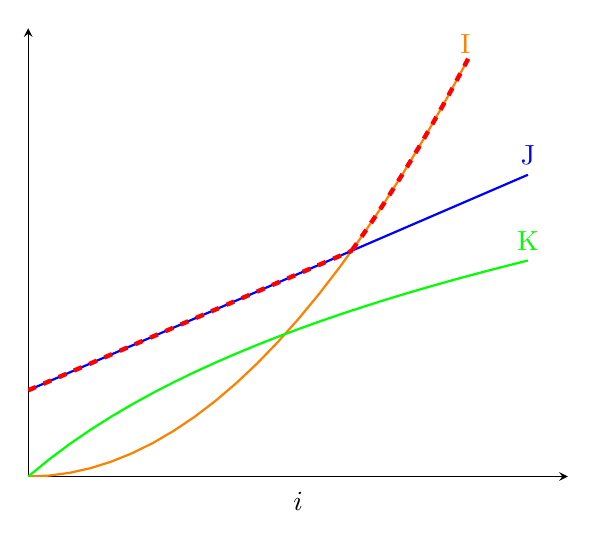
\begin{tikzpicture}
\begin{axis}[
    axis lines = left,
    xlabel = \(i\),
    ylabel = {},
    domain = 0:2.5,
    xtick={\empty},ytick={\empty},
    ymin=0,
    ymax=5.2,
    xmax=2.7,
    restrict y to domain=0:5,
]
    \addplot[thick, color=orange]{x^2} node[above,pos=1] {I};
    \addplot[thick, color=blue]{x+1} node[above,pos=1] {J};
    \addplot[thick, color=green]{ln(x+1)*2} node[above,pos=1] {K};
    \draw [ultra thick, dashed, draw=red] (axis cs:0,1) -- (axis cs:1.62,2.62);
    \addplot[ultra thick, color=green, dashed, color=red, domain=1.62:2.5]{x^2};
\end{axis}
\end{tikzpicture}
    
    \caption{Combined complexities illustrated. The combined complexity consists of the three indices I, J, K of the single index variable $i$. The dashed red line shows the bound of the combined complexity. $K$ is a superfluous index in the combined complexity as it never contributes to the bound of the combined complexity.}
    \label{fig:combined_complexity}
\end{figure}


\begin{definition}[Combined complexity]\label{def:combinedcomp} 
    We refer to a set $\kappa$ of complexities as a \textit{combined complexity}. We extend constraint judgements to include combined complexities such that
    \begin{enumerate}
        \item $\varphi;\Phi\vDash \kappa \leq \kappa'$ if for all $K \in \kappa$ there exists $K'\in \kappa'$ such that $\varphi;\Phi\vDash K \leq K'$.
        % 
        \item $\varphi;\Phi\vDash \kappa = \kappa'$ if $\varphi;\Phi\vDash \kappa \leq \kappa'$ and $\varphi;\Phi\vDash \kappa' \leq \kappa$.
        \item $\kappa + I = \{K + I \mid K \in \kappa\}$.
        %
        \item $\kappa\{J/i\} = \{ K\{J/i\} \mid K\in\kappa \}$.
    \end{enumerate}
    In the above, we may substitute an index for a combined complexity. In such judgements, the index represents a singleton set. For instance, $\varphi;\Phi\vDash \kappa \leq K$ represents $\varphi;\Phi\vDash \kappa \leq \{K\}$.
    %$\varphi;\Phi \vDash \kappa \bowtie \kappa' \quad\text{ if }\quad \forall K \in \kappa. (\exists K' \in \kappa'. \varphi;\Phi \vDash K \bowtie K')$.
\end{definition}

More specifically, when considering a combined complexity $\kappa$, we are interested in the maximal complexity given some valuation $\rho$, which we find by simply comparing the different values for the complexities within $\kappa$ given $\rho$. Note that the complexity $K \in \kappa$ that is maximal may be different for different valuations. In Definition \ref{def:combinedcomp} we extend the binary relations in $\bowtie$ on indices to combined complexities, such that we can compare two combined complexities such as $\varphi;\Phi \vDash \kappa \bowtie \kappa'$ and a combined complexity and complexity such as $\varphi;\Phi \vDash \kappa \bowtie K$. Definition \ref{def:combinedcompbasis} defines the function \textit{basis} that discards any $K \in \kappa$ that can never be the maximal complexity given some set of constraints $\Phi$ (i.e. the complexities that are bounded by other complexities in the set), such that we can always keep the number of complexities in a combined complexity to a minimum. %Finally, we may also be interested in adding an index onto a combined complexity, and so we define the addition of indices onto combined complexities in Definition \ref{def:combinedcompadd}.
%
\begin{definition}\label{def:combinedcompbasis}
    We define the function \textit{basis} that takes a set of index variables $\varphi$, a set of constraints $\Phi$ and a combined complexity $\kappa$, and returns a new combined complexity without superfluous complexities (The \textit{basis} of $\kappa$)
    \begin{align*}
        \text{basis}(\varphi,\Phi,\kappa) = \bigcap\left\{ \kappa' \subseteq \kappa \mid \forall K\in\kappa.\exists K'\in\kappa'.\varphi;\Phi\vDash K \leq K' \right\}
    \end{align*}
    Moreover, the algorithm below computes the basis
    % \begin{align*}
    %     \text{basis}(\varphi, \kappa) = \{(\Phi, K) \in \kappa \mid \varphi;\Phi \not \vDash K < K' \text{ for all } (\Phi', K') \in \kappa\}
    % \end{align*}
    \begin{align*}
        &\text{basis}(\varphi, \Phi, \kappa) = \text{do}\\[-0.5em]
        &\quad \kappa' \leftarrow \kappa\\[-0.5em]
        &\quad \text{for } K \in \kappa \text{ do}\\[-0.5em]
        &\quad\quad \text{ if } \exists K' \in \kappa' \text{ with } K \not = K' \text{ and } \varphi;\Phi \vDash K \leq K' \text{ then}\\[-0.5em]
        &\quad\quad\quad \kappa' \leftarrow \kappa' \setminus \{K\}\\[-0.5em]
        &\quad \text{return } \kappa'
    \end{align*}
\end{definition}
%
% \begin{definition}[]\label{def:combinedcompadd}
%     We define the the addition of a combined complexity and index as
%     \begin{align*}
%         \kappa + I = \{K + I \mid K \in \kappa\}
%     \end{align*}

% \end{definition}
%
For typing expressions, we use the rules presented in Table \ref{tab:sizedtypedexpressiontypes}, excluding the rule $\runa{BG-sub}$. In Table \ref{tab:sizedprocesstypingrules} we show the type rules for processes. Type judgements are of the form $\varphi;\Phi;\Gamma \vdash P \triangleleft \kappa$ where $\kappa$ denotes the complexity of process $P$. The rule $\runa{S-tick}$ types a \texttt{tick} prefix and incurs a cost of one in time complexity. We advance the time of all types in the context accordingly when typing the continuation. Rule $\runa{S-annot}$ is similar but may incur a cost of $n$. Matches on naturals are typed with rule $\runa{S-nmatch}$. Most notably, we extend the set of known constraints when typing the two continuations. That is, we can deduce constraints on the lower and upper bounds on the size of the expression we match on. For instance, for the zero pattern we can deduce that the lower bound $I$ must be equal to $0$ (or equivalently $I \leq 0$), and for the successor pattern, we can guarantee that the upper bound $J$ must be greater than or equal to $1$. For the complexity of pattern matches and parallel composition, we take advantage of the fact that we represent complexities using combined complexities. As such, we include complexities in both $P$ and $Q$ in the result. To remove redundancy from the set $\kappa \cup \kappa'$, we use the basis function.\\

%
% \begin{table*}[!ht]
%     \begin{framed}\vspace{-1em}\begin{align*}
%         &\kern15em\\[-2em] % Stretch frame
%         &\kern0em\runa{S-nil}\infrule{}{\varphi;\Phi;\Gamma \vdash \withcomplex{\nil}{0}} \kern1em\runa{S-tick}\;\infrule{\varphi;\Phi;\susumesim{\Gamma}{1}\vdash P \triangleleft K}{\varphi;\Phi;\Gamma\vdash \tick P \triangleleft K + 1} \kern3em\runa{S-nu}\;\infrule{\varphi;\Phi;\Gamma,\withtype{a}{T} \vdash \withcomplex{P}{K}}{\varphi;\Phi;\Gamma \vdash \newvar{a: T}{\withcomplex{P}{K}}}\\[-1em]
%         %
%         &\kern-0em\runa{S-nmatch}\;\condinfrule{
%         \begin{matrix}
%             \varphi;\Phi;\Gamma \vdash \withtype{e}{\natinterval{I}{J}}\quad \varphi;\Phi, I \leq 0;\Gamma \vdash \withcomplex{P}{K} \\
%             \varphi;\Phi, J \geq 1;\Gamma, \withtype{x}{\natinterval{I-1}{J-1}} \vdash \withcomplex{Q}{K'}
%         \end{matrix}}{\varphi;\Phi;\Gamma \vdash \withcomplex{\match{e}{P}{x}{Q}}{L}}{\text{where}\quad L = \left\{
% \begin{matrix}
%     K & \text{if}\; \varphi;\Phi\vDash K' \leq K   \\
%     K' & \text{if}\; \varphi;\Phi\vDash K \leq K'  \\
%     K+K' & \text{otherwise}
% \end{matrix}
% \right.}\\[-1em]
%         %
%         %&\kern-0em\runa{S-nmatch-2}\;\infrule{
%         %\begin{matrix}
%         %    \varphi;\Phi;\Gamma \vdash \withtype{e}{\natinterval{I}{J}} \quad \varphi;\Phi\vDash K \leq K' \\
%         %    \varphi;\Phi, I \leq 0;\Gamma \vdash \withcomplex{P}{K} \quad \varphi;\Phi, J \geq 1;\Gamma, \withtype{x}{\natinterval{I-1}{J-1}} \vdash \withcomplex{Q}{K'}
%         %\end{matrix}}{\varphi;\Phi;\Gamma \vdash \withcomplex{\match{e}{P}{x}{Q}}{K'}}\\[-1em]
%         %
%         &\kern-0em\runa{S-lmatch}\;\condinfrule{
%         \begin{matrix}
%             \varphi;\Phi;\Gamma \vdash \withtype{e}{\texttt{List}[I,J](\mathcal{B})} \quad \varphi;\Phi, I \leq 0;\Gamma \vdash \withcomplex{P}{K} \\
%             \varphi;\Phi, J \geq 1;\Gamma, \withtype{x}{\mathcal{B}},y : \texttt{List}[I-1,J-1](\mathcal{B}) \vdash \withcomplex{Q}{K'}
%         \end{matrix}}{\varphi;\Phi;\Gamma \vdash \withcomplex{\texttt{match}\;e\;\{ [] \mapsto P;\; x :: y \mapsto Q \}}{L}}{\text{where}\quad L = \left\{
% \begin{matrix}
%     K & \text{if}\; \varphi;\Phi\vDash K' \leq K   \\
%     K' & \text{if}\; \varphi;\Phi\vDash K \leq K'  \\
%     K+K' & \text{otherwise}
% \end{matrix}
% \right.}\\[-1em]
%         %
%         %&\kern-0em\runa{S-lmatch-2}\;\infrule{
%         %\begin{matrix}
%         %    \varphi;\Phi;\Gamma \vdash \withtype{e}{\texttt{List}[I,J](\mathcal{B})} \quad \varphi;\Phi\vDash K \leq K' \\
%         %    \varphi;\Phi, I \leq 0;\Gamma \vdash \withcomplex{P}{K} \quad \varphi;\Phi, J \geq 1;\Gamma, \withtype{x}{\mathcal{B}},y : \texttt{List}[I-1,J-1](\mathcal{B}) \vdash \withcomplex{Q}{K'}
%       % \end{matrix}}{\varphi;\Phi;\Gamma \vdash \withcomplex{\texttt{match}\;e\;\{ [] \mapsto P;\; x :: y \mapsto Q \}}{K'}}\\[-1em]
%         %
%         &\kern4em\runa{S-par}\;\condinfrule{\varphi;\Phi;\Gamma\vdash P \triangleleft K\quad \varphi;\Phi;\Gamma\vdash Q \triangleleft K'}{\varphi;\Phi;\Gamma\vdash \parcomp{P}{Q} \triangleleft L}{\text{where}\quad L = \left\{
% \begin{matrix}
%     K & \text{if}\; \varphi;\Phi\vDash K' \leq K   \\
%     K' & \text{if}\; \varphi;\Phi\vDash K \leq K'  %\\
%     %K+K' & \text{otherwise}
% \end{matrix}
% \right.}\\[-1em]
%         %
%         %&\kern4em\runa{S-par-2}\;\infrule{\varphi;\Phi;\Gamma\vdash P \triangleleft K\quad \varphi;\Phi;\Gamma\vdash Q \triangleleft K'\quad \varphi;\Phi\vDash K \leq K'}{\varphi;\Phi;\Gamma\vdash \parcomp{P}{Q} \triangleleft K'}\\[-1em]
%         %
%         &\kern-0em\runa{S-iserv}\;\infrule{\texttt{in}\in\sigma\quad \varphi,\widetilde{i};\Phi;\text{ready}(\varphi,\Phi,\susumesim{\Gamma}{I}),a:\forall_0\widetilde{i}.\texttt{serv}^{\sigma\cap\{\texttt{out}\}}_K(\widetilde{T}),\widetilde{v} : \widetilde{T}\vdash P \triangleleft K'\quad \varphi,\widetilde{i};\Phi\vDash K' \leq K}{\varphi;\Phi;\Gamma,a:\forall_I\widetilde{i}.\texttt{serv}^\sigma_K(\widetilde{T})\vdash\; \bang\inputch{a}{\widetilde{v}}{}{P}\triangleleft I}\\[-1em]
%         %
%         &\kern-0em\runa{S-ich}\;\infrule{\texttt{in}\in\sigma\quad \varphi;\Phi;\susumesim{\Gamma}{I},a:\texttt{ch}_0^\sigma(\widetilde{T}),\widetilde{v} : \widetilde{T}\vdash P \triangleleft K}{\varphi;\Phi;\Gamma,a:\texttt{ch}_I^\sigma(\widetilde{T})\vdash \inputch{a}{\widetilde{v}}{}{P}\triangleleft K + I}
%         %
%         \kern8.5em \runa{S-och}\;\infrule{\texttt{out}\in \sigma\quad \varphi;\Phi;\susumesim{\Gamma}{I}\vdash \widetilde{e} : \widetilde{T}\quad \varphi;\Phi\vdash\widetilde{T}\sqsubseteq\widetilde{S}}{\varphi;\Phi;\Gamma,a:\texttt{ch}^{\sigma}_I(\widetilde{S})\vdash \asyncoutputch{a}{\widetilde{e}}{} \triangleleft I}\\[-1em]
%         %
%         &\kern0em\runa{S-oserv}\;\infrule{\texttt{out} \in \sigma \quad \varphi;\Phi;\susumesim{\Gamma}{I}\vdash \widetilde{e} : \widetilde{T}\quad \text{instantiate}(\widetilde{i},\widetilde{T})=\{\widetilde{J}/\widetilde{i}\}\quad  \varphi;\Phi\vdash\widetilde{T}\sqsubseteq\widetilde{S}\{\widetilde{J}/\widetilde{i}\}}{\varphi;\Phi;\Gamma,a:\forall_I\widetilde{i}.\texttt{serv}_K^\sigma(\widetilde{S})\vdash \asyncoutputch{a}{\widetilde{e}}{} \triangleleft K\!\substi{\widetilde{J}}{\widetilde{i}} + I}
%         %
%     \end{align*}\vspace{-1em}\end{framed}
%     \smallskip
%     \caption{Sized typing rules for parallel complexity of processes.}
%     \label{tab:sizedprocesstypingrules}
% \end{table*}

\begin{table*}[!ht]
    \begin{framed}\vspace{-1em}\begin{align*}
        %
        % S-nil
        &\runa{S-nu}\infrule{\varphi;\Phi;\Gamma, a:T \vdash P \triangleleft \kappa}{\varphi;\Phi;\Gamma \vdash \newvar{a:T}{P} \triangleleft \kappa}
        % S-par
        \kern1em\runa{S-par}\infrule{\varphi;\Phi;\Gamma \vdash P \triangleleft \kappa \quad \varphi;\Phi;\Gamma \vdash Q \triangleleft \kappa'}{\varphi;\Phi;\Gamma \vdash P \mid Q \triangleleft \text{basis}(\varphi, \Phi,\kappa \cup \kappa')}\\[-1em]
        %
        &\runa{S-tick}\infrule{\varphi;\Phi;\tforwardsim{\Gamma}{1} \vdash P \triangleleft \kappa}{\varphi;\Phi;\Gamma \vdash \tick P \triangleleft \kappa + 1}\kern2em
        %
        \runa{S-annot}\infrule{\varphi;\Phi;\tforwardsim{\Gamma}{n}\vdash P \triangleleft \kappa}{\varphi;\Phi;\Gamma\vdash n:P \triangleleft \kappa + n}\\[-1em]
        % S-match
        &\runa{S-match}\infrule{
        \begin{matrix}
            \varphi;\Phi;\Gamma \vdash e:\natinterval{I}{J} \quad \varphi;\Phi, I \leq 0;\Gamma \vdash P \triangleleft \kappa\\
            \varphi;\Phi, J \geq 1;\Gamma, x:\natinterval{I-1}{J-1} \vdash Q \triangleleft \kappa'
        \end{matrix}}{\varphi;\Phi;\Gamma \vdash \match{e}{P}{x}{Q} \triangleleft \text{basis}(\varphi, \Phi, \kappa \cup \kappa')}\\[-1em]
        % S-iserv
        &\runa{S-iserv}\infrule{\begin{matrix}
            \texttt{in} \in \sigma\quad \varphi;\Phi;\Gamma\vdash a:\servt{I}{i}{\sigma}{K}{\widetilde{T}}\\
            \varphi, \widetilde{i}; \Phi; \text{ready}(\varphi,\Phi,\tforwardsim{\Gamma}{I}), \widetilde{v} : \widetilde{T} \vdash P \triangleleft \kappa \quad \varphi,\widetilde{i};\Phi\vDash\kappa \leq K
        \end{matrix}}
        {\varphi;\Phi;\Gamma \vdash \;\bang\inputch{a}{\widetilde{v}}{}{P}\triangleleft \{I\}}
        %
        \kern14em\runa{S-nil}\kern-1em\infrule{}{\varphi;\Phi;\Gamma \vdash \nil \triangleleft \{0\}}\kern-3em\text{ }\\[-1em]
        % S-oserv
        &\runa{S-oserv}\infrule{\begin{matrix}
            \texttt{out} \in \sigma\quad \varphi;\Phi;\Gamma\vdash a:\servt{I}{i}{\sigma}{K}{\widetilde{T}}\\
            \varphi; \Phi;\tforwardsim{\Gamma}{I} \vdash \widetilde{e}:\widetilde{S} \quad \text{instantiate}(\widetilde{i}, \widetilde{S}) = \{\widetilde{J}/\widetilde{i}\} \quad \varphi;\Phi \vDash \widetilde{S} \sqsubseteq \widetilde{T}
        \end{matrix}}
        {\varphi;\Phi;\Gamma \vdash \asyncoutputch{a}{\widetilde{e}}{}\triangleleft \{K\{\widetilde{J}/\widetilde{i}\} + I\}}\\[-1em]
        % S-annot
        &\runa{S-ich}\infrule{\begin{matrix}
            \texttt{in} \in \sigma\quad \varphi;\Phi;\Gamma \vdash a:\chant{\sigma}{I}{\widetilde{T}}\\
            \varphi; \Phi; \tforwardsim{\Gamma}{I}, \widetilde{v}:\widetilde{T} \vdash P \triangleleft \kappa
        \end{matrix}}
        {\varphi;\Phi;\Gamma \vdash \inputch{a}{\widetilde{v}}{}{P} \triangleleft \kappa + I}\kern3em
        %
        \runa{S-och}\infrule{\begin{matrix}
            \texttt{out} \in \sigma\quad \varphi;\Phi;\Gamma \vdash a:\chant{\sigma}{I}{\widetilde{T}}\\
            \varphi; \Phi; \tforwardsim{\Gamma}{I} \vdash \widetilde{e}:\widetilde{S} \quad \varphi;\Phi \vDash \widetilde{S} \sqsubseteq \widetilde{T}
        \end{matrix}}
        {\varphi;\Phi;\Gamma \vdash \asyncoutputch{a}{\widetilde{e}}{} \triangleleft \{I\}}\\[-1em]
    \end{align*}\vspace{-1em}\end{framed}
    \smallskip
    \caption{Sized typing rules for parallel complexity of processes.}
    \label{tab:sizedprocesstypingrules}
\end{table*}

%
Rule $\runa{S-iserv}$ types a replicated input on a name $a$, and so $a$ must be bound to a server type with input capability. As the index $I$ in the server type denotes the time steps remaining before the server is ready to synchronize, we advance the time by $I$ units of time complexity when typing the continuation $P$. To ensure that bounds on synchronizations in $\downarrow^{\varphi;\Phi}_I\!\Gamma$ are not violated, we type $P$ under the time invariant part of $\downarrow^{\varphi;\Phi}_I\!\Gamma$, i.e. $\text{ready}(\varphi,\Phi,\downarrow_I\!\Gamma)$. Note that the bound on the span of the replicated input is the bound on the time remaining before the server is ready to synchronize. As the replicated input may be invoked many times, the cost of invoking the server is accounted for in rule $\runa{S-oserv}$ using the complexity bound $K$ in the server type. Therefore, we enforce that $K$ is in fact an upper bound on the span of the continuation $P$.\\

The rule $\runa{S-oserv}$ types outputs on names bound to server types. Here, as stated above, we must account for the cost of invoking a server, and as a replicated input on a server is parametric, we must \textit{instantiate} it based on the types of the expressions we are to output. Recall that in the type rule for outputs on servers from Chapter \ref{ch:bgts}, this is to be done by finding a substitution that satisfies the premise $\widetilde{T} \sqsubseteq \widetilde{S}\{\widetilde{J}/\widetilde{i}\}$. However, this turns out to be a difficult problem, and we can in fact prove it NP-complete for types of polynomial indices even if we disregard subtyping. However, note that it might not be necessary to use the full expressive power of polynomial indices, and so this may not necessarily affect type checking. Nevertheless, we over-approximate finding such a substitution, by using the function $\textit{instantiate}$. That is, we \textit{zip} together the index variables $\widetilde{i}$ with indices in types $\widetilde{T}$. Remark that Baillot and Ghyselen \cite{BaillotGhyselen2021} propose types for inference in their technical report, where the problem is simplified substantially, by forcing naturals to have lower bounds of $0$ and upper bounds with exactly one index variable and a constant. Our approach admits more expressive lower bounds and multiplications, while imposing no direct restrictions on the number of index variables in an index, and is thus more suitable for a type-checker.\\

We now prove the NP-completeness of the smaller problem of checking whether there exists a substitution $\{\widetilde{J}/\widetilde{i}\}$ that satisfies $T = S\{\widetilde{J}/\widetilde{i}\}$ where $T$ and $S$ are types with polynomial indices. The main idea is a reduction proof from the NP-complete 3-SAT problem, i.e. the satisfiability problem of a boolean formula in conjunctive normal form with exactly three literals in each clause \cite{Karp1972}. We first define a translation from a 3-SAT formula to a polynomial index in Definition \ref{def:3satredu}. This is a polynomial time computable reduction, as we simply replace each logical-and with a multiplication, each logical-or with an addition and each negation with a subtraction from 1. In Lemma \ref{lemma:soundtranslation}, we prove that the reduction is faithful with respect to satisfiability of a boolean formula. Finally, in Lemma \ref{lemma:npcompletesubst}, we prove that it is an NP-complete decision problem to verify the existence of a substitution that satisfies $T = S\{\widetilde{J}/\widetilde{i}\}$ for types $T$ and $S$.
%
\begin{definition}[3-SAT reduction]\label{def:3satredu}
We assume a one-to-one mapping $f$ from unknowns to index variables. Let $\phi$ be a 3-SAT formula
\begin{align*}
    \phi = \bigwedge_{i=1}^n \left(\ell_{i1} \lor \ell_{i2} \lor \ell_{i3}\right)% \land \cdots \land (A_n \lor B_n \lor C_n)
\end{align*}
where $\ell_{i1}$, $\ell_{i2}$ and $\ell_{i3}$ are of the forms $x$ or $\neg x$ for some variable $x$. We define a translation of $\phi$ to a polynomial index %$[\![\phi]\!]_{\text{3-SAT}}$
\begin{align*}
    [\![\phi]\!]_{\text{3-SAT}} = \prod_{i=1}^n \left([\![\ell_{i1}]\!]_{\text{3-SAT}} + [\![\ell_{i2}]\!]_{\text{3-SAT}} + [\![\ell_{i3}]\!]_{\text{3-SAT}}\right) %\cdots ([\![A_n]\!]_{\text{3-SAT}} + [\![B_n]\!]_{\text{3-SAT}} + [\![C_n]\!]_{\text{3-SAT}})
\end{align*}
where $[\![x]\!]_{\text{3-SAT}} = f(x)$ and $[\![\neg x]\!]_{\text{3-SAT}} = (1 - f(x))$.
\end{definition}


\begin{lemma}\label{lemma:soundtranslation}
Let $\phi$ be a 3-SAT formula. Then $\phi$ is satisfiable if and only if there exists a substitution $\{\widetilde{n}/\widetilde{i}\}$ such that $1\leq [\![\phi]\!]_{\text{3-SAT}}\{\widetilde{n}/\widetilde{i}\}$.
\begin{proof}
We consider the implications separately
\begin{enumerate}
    \item Assume that $\phi$ is satisfiable. Then there exists a truth assignment $\tau$ such that each clause of $\phi$ is true. Correspondingly, as $[\![\phi]\!]_{\text{3-SAT}}$ is a product of non-negative factors, we for some substitution $\{\widetilde{n}/\widetilde{i}\}$ have that $1 \leq [\![\phi]\!]_{\text{3-SAT}}\{\widetilde{n}/\widetilde{i}\}$ if and only if each factor in the product is positive. We compare the conditions for a clause to be true in $\phi$ to those for a corresponding factor in $[\![\phi]\!]_{\text{3-SAT}}$ to be positive, and show that a substitution $\{\widetilde{n}/\widetilde{i}\}$ exists such that $1 \leq [\![\phi]\!]_{\text{3-SAT}}\{\widetilde{n}/\widetilde{i}\}$. A clause in $\phi$ is a disjunction of three literals of either the form $x$ or $\neg x$ for some unknown $x$. Thus, for a clause to be true, we must have at least one literal $\tau(x) = tt$ or $\neg \tau(x) = tt$ with $\tau(x) = f\!f$. The corresponding factor in $[\![\phi]\!]_{\text{3-SAT}}$ is a sum of three terms of the forms $f(x)$ or $(1 - f(x))$ for some unknown $x$, where $f$ is a one-to-one mapping from unknowns to index variables. Here, we utilize that in the type system by Baillot and Ghyselen \cite{BaillotGhyselen2021}, we have $(1 - i\{\widetilde{n}/\widetilde{i}\}) = 0$ when $i\{\widetilde{n}/\widetilde{i}\} \geq 1$ and $(1 - i\{\widetilde{n}/\widetilde{i}\}) = 1$ when $i\{\widetilde{n}/\widetilde{i}\} = 0$. Thus, for a factor to be positive, it suffices that one term is positive, and so we can construct a substitution that guarantees this from the interpretation of $\phi$. That is, if $\tau(x) = tt$, we substitute $1$ for $f(x)$, and if $\tau(x) = f\!f$, we substitute 0 for $f(x)$. Then, whenever a literal is true in $\phi$, the corresponding term in $[\![\phi]\!]_{\text{3-SAT}}$ is positive, and so if $\phi$ is satisfiable then there exists a substitution $\{\widetilde{n}/\widetilde{i}\}$ such that $1 \leq [\![\phi]\!]_{\text{3-SAT}}\{\widetilde{n}/\widetilde{i}\}$.
     
    \item Assume that there exists a substitution $\{\widetilde{n}/\widetilde{i}\}$ such that $1 \leq [\![\phi]\!]_{\text{3-SAT}}\{\widetilde{n}/\widetilde{i}\}$. Then, as $[\![\phi]\!]_{\text{3-SAT}}$ is a product of non-negative factors, each factor must be positive. Correspondingly, if $\Phi$ is satisfiable, then there exists a truth assignment such that each clause of $\phi$ is true. We compare the conditions for a factor in $[\![\phi]\!]_{\text{3-SAT}}\{\widetilde{n}/\widetilde{i}\}$ to be positive to those for a corresponding clause in $\phi$ to be true, and show that $\phi$ is satisfiable. A factor in $[\![\phi]\!]_{\text{3-SAT}}$ is a sum of at most three terms of the forms $f(x)\{\widetilde{n}/\widetilde{i}\}$ or $(1 - f(x)\{\widetilde{n}/\widetilde{i}\})$. Here we again utilize that in the type system by Baillot and Ghyselen \cite{BaillotGhyselen2021}, we have $(1 - f(x)\{\widetilde{n}/\widetilde{i}\}) = 0$ when $f(x)\{\widetilde{n}/\widetilde{i}\} \geq 1$ and $(1 - f(x)\{\widetilde{n}/\widetilde{i}\}) = 1$ when $f(x)\{\widetilde{n}/\widetilde{i}\} = 0$, and so it must be that in the factor, we have at least one term $f(x)\{\widetilde{n}/\widetilde{i}\} \geq 1$ or $(1 - f(x)\{\widetilde{n}/\widetilde{i}\}) \geq 1$. Correspondingly, for the clause in $\phi$ to be true, at least one literal must be true. We show that there exists a truth assignment $\tau$ such that if a term in $[\![\phi]\!]_{\text{3-SAT}}$ is positive, then the corresponding literal in $\phi$ is true. If $f(x)\{\widetilde{n}/\widetilde{i}\}\geq 1$ then we set $\tau(x) = tt$, and if $f(x)\{\widetilde{n}/\widetilde{i}\} = 0$ we set $\tau(x) = f\!f$, as $[\![x]\!]_{\text{3-SAT}}\{\widetilde{n}/\widetilde{i}\} \geq 1$ when $f(x)\{\widetilde{n}/\widetilde{i}\} \geq 1$ and $[\![\neg x]\!]_{\text{3-SAT}} \geq 1$ when $f(x)\{\widetilde{n}/\widetilde{i}\}=0$. Then, whenever a term is positive in $[\![\phi]\!]_{\text{3-SAT}}\{\widetilde{n}/\widetilde{i}\}$, the corresponding literal in $\phi$ is true, and so if there exists a substitution $\{\widetilde{n}/\widetilde{i}\}$ such that $1 \leq [\![\phi]\!]_{\text{3-SAT}}\{\widetilde{n}/\widetilde{i}\}$, then $\phi$ is satisfiable.
    
\end{enumerate}
\end{proof}
\end{lemma}


\begin{lemma}\label{lemma:npcompletesubst}
Let $T$ and $S$ be types with polynomial indices. Then checking whether there exists a substitution $\{\widetilde{J}/\widetilde{i}\}$ such that $T = S\{\widetilde{J}/\widetilde{i}\}$ is an NP-complete problem.
\begin{proof}
By reduction from the 3-SAT problem. Assume that we have some algorithm that can verify the existence of a substitution $\{\widetilde{J}/\widetilde{i}\}$ such that $T = S\{\widetilde{J}/\widetilde{i}\}$, and let $\phi$ be a 3-SAT formula. Then using the algorithm, we can check whether $\phi$ is satisfiable by verifying whether there exists $\{\widetilde{J}/\widetilde{i}\}$ such that the following holds
\begin{align*}
    \texttt{Nat}[0,1] = \texttt{Nat}[0,(1 - (1 - [\![\phi]\!]_{\text{3-SAT}}))]\{\widetilde{J}/\widetilde{i}\}
\end{align*}
That is, $1 = (1 - (1 - [\![\phi]\!]_{\text{3-SAT}}\{\widetilde{J}/\widetilde{i}\}))$ implies $1 \leq [\![\phi]\!]_{\text{3-SAT}}\{\widetilde{J}/\widetilde{i}\}$, as $(1 - [\![\phi]\!]_{\text{3-SAT}}\{\widetilde{J}/\widetilde{i}\}) = 0$ when $[\![\phi]\!]_{\text{3-SAT}}\{\widetilde{J}/\widetilde{i}\} \geq 1$ and $(1 - [\![\phi]\!]_{\text{3-SAT}}\{\widetilde{J}/\widetilde{i}\}) = 1$ when $[\![\phi]\!]_{\text{3-SAT}}\{\widetilde{J}/\widetilde{i}\} = 0$. Furthermore, for $1 \leq [\![\phi]\!]_{\text{3-SAT}}\{\widetilde{J}/\widetilde{i}\}$ to hold, the indices in the sequence $\widetilde{J}$ cannot contain index variables, and so there must exist an equivalent substitution of naturals for index variables $\{\widetilde{n}/\widetilde{i}\}$. Then, by Lemma \ref{lemma:soundtranslation} we have that $\phi$ is satisfiable if and only if there exists a substitution $\{\widetilde{n}/\widetilde{i}\}$ such that $1\leq [\![\phi]\!]_{\text{3-SAT}}\{\widetilde{n}/\widetilde{i}\}$. Thus, as 3-SAT is an NP-complete problem, the reduction from 3-SAT is computable in polynomial time and as polynomial reduction is a transitive relation, i.e. any NP-problem is polynomial time reducible to verifying the existence of a substitution $\{\widetilde{J}/\widetilde{i}\}$ that satisfies the equation $T = S\{\widetilde{J}/\widetilde{i}\}$, it follows that the problem is NP-hard. To show that it is an NP-complete problem, we show that a \textit{certificate} can be verified in polynomial time. That is, given some substitution $\{\widetilde{J}/\widetilde{i}\}$, we can in linear time check whether $T=S\{\widetilde{J}/\widetilde{i}\}$ by substituting indices $\widetilde{J}$ for indices $\widetilde{i}$ in type $S$ and by then comparing the two types.\\
%
%
%Utilizing that $n - m = 0$ for $m\geq n$ in the type system of Baillot and Ghyselen \cite{BaillotGhyselen2021}, we can simulate any boolean formula using a polynomial index. By denoting $J = 0$ false and $I > 0$ true, we have the translation
% \begin{align*}
%     [\![a \land b]\!]_\phi =&\; [\![a]\!]_\phi [\![b]\!]_\phi\\
%     [\![a \lor b]\!]_\phi =&\; [\![a]\!]_\phi + [\![b]\!]_\phi\\
%     [\![\neg a]\!]_\phi =&\; (1 - [\![a]\!]_\phi)\\
%     [\![x]\!]_\phi =&\; i
% \end{align*}
% Then assuming some algorithm that checks whether there exists a substitution $\{\widetilde{J}/\widetilde{i}\}$ such that $T \sqsubseteq S\{\widetilde{J}/\widetilde{i}\}$, we can solve the boolean satisfiability problem. Let $\phi_0$ be any boolean formula and let $\widetilde{i}$ be the index variables in $[\![\phi_0]\!]_\phi$, and assume that there exists a substitution $\{\widetilde{J}/\widetilde{i}\}$ that satisfies the judgement
% \begin{align*}
%     \emptyset;\emptyset\vDash\texttt{Nat}[0,1] \sqsubseteq \texttt{Nat}[0,[\![\phi_0]\!]_\phi]\{\widetilde{J}/\widetilde{i}\}
% \end{align*}
% Then by rule $\runa{SS-nweak}$ we have that $\emptyset;\emptyset\vDash 1 \leq [\![\phi_0]\!]_\phi\{\widetilde{J}/\widetilde{i}\}$, and as $\varphi = \emptyset$, the indices $\widetilde{J}$ must be constants. Thus, $\emptyset;\emptyset\vDash 1 \leq [\![\phi_0]\!]_\phi\{\widetilde{J}/\widetilde{i}\}$ is equivalent to $1 \leq [\![\phi_0]\!]_\phi\{\widetilde{J}/\widetilde{i}\}$, and so $\phi_0$ must have a solution. If instead no such substitution exists, then for any $\{\widetilde{J}/\widetilde{i}\}$, it must be that $[\![\phi_0]\!]_\phi\{\widetilde{J}/\widetilde{i}\} = 0$ implying that $\phi_0$ is a contradiction. Therefore, as the boolean satisfiability problem is NP-complete, the algorithm we assumed must be NP-complete as well.
\end{proof}
\end{lemma}

In Example \ref{example:addition}, we show how a process implementing addition of naturals can be typed using our type rules, yielding a precise bound on the parallel complexity.
%

\begin{example}\label{example:addition}
As an example of a process that is typable using our type rules, we show how the addition operator for naturals can be written as a process and subsequently be typed. We use a server to encode the addition operator
\begin{align*}
    !\inputch{\text{add}}{x,y,r}{}{\match{x}{\asyncoutputch{r}{y}{}}{z}{\tick{\asyncoutputch{\text{add}}{z,\succc y,r}{}}}}
\end{align*}
such that channel $r$ is used to output the addition of naturals $x$ and $y$. To type the process, we use the following contexts and set of index variables
\begin{align*}
    \Gamma\defeq&\; \text{add} : \forall_0 i,j,k,l,m,n,o.\texttt{serv}^{\{\texttt{in},\texttt{out}\}}_j(\texttt{Nat}[0,j],\texttt{Nat}[0,l],\texttt{ch}^{\{\texttt{out}\}}_j(\texttt{Nat}[0,j+l])) \\
    \Delta\defeq&\; \text{ready}(\cdot,\cdot,\Gamma), x : \texttt{Nat}[0,j], y: \texttt{Nat}[0,l], r:\texttt{ch}^{\{\texttt{out}\}}_j(\texttt{Nat}[0,j+l])\\
    \varphi \defeq&\; \{i,j,k,l,m,n,o\}
\end{align*}
%
We now derive a type for the encoding of the addition operator, yielding a precise bound of $j$, corresponding to an upper bound on the size of $x$, as we pattern match at most $j$ times on natural $x$. Notably we have that $\text{instantiate}((i,j,k,l,m,n,o),\texttt{Nat}[0,j\monus 1],\texttt{Nat}[1,l+1],\texttt{ch}^{\{\texttt{out}\}}_j(\texttt{Nat}[0,j+l]))=\{0/i,j\monus 1/j,0/k,l+1/l,j/m,0/n,j+l/o\}$.
%
% {\small
% \begin{align*}
%     \begin{prooftree}
%         %
%         \infer0{\varphi;\cdot,0\leq 0;\Delta\vdash \asyncoutputch{r}{y}{} \triangleleft \{j\}}
%         %
%         % \infer0{\texttt{Nat}[0,j\monus 1] \sqsubseteq \texttt{Nat}[0,j]\{j\monus 1/j\}}
%         % %
%         % \infer0{\texttt{Nat}[0,l+1] \sqsubseteq \texttt{Nat}[0,l]\{l+1/l\}}
%         % %
%         % \infer0{\texttt{ch}^{\{\texttt{out}\}}_{j\monus 1}(\texttt{Nat}[0,j+l] \sqsubseteq \texttt{ch}^{\{\texttt{out}\}}_{j\monus 1}(\texttt{Nat}[0,j+l)\{j\monus 1/j,l+1/l\}}
%         %
%         \infer0{
%         \begin{matrix}
%         \varphi;\cdot,1\leq j\vdash\texttt{Nat}[0,j\monus 1] \sqsubseteq \texttt{Nat}[0,j]\{j\monus 1/j\}\\
%         \varphi;\cdot,1\leq j\vdash\texttt{Nat}[1,l+1] \sqsubseteq \texttt{Nat}[0,l]\{l+1/l\}\\
%         \varphi;\cdot,1\leq j\vdash\texttt{ch}^{\{\texttt{out}\}}_{j\monus 1}(\texttt{Nat}[0,j+l] \sqsubseteq \texttt{ch}^{\{\texttt{out}\}}_{j\monus 1}(\texttt{Nat}[0,j+l)\{j\monus 1/j,l+1/l\}
%         \end{matrix}
%         }
%         %
%         \infer1{\varphi;\cdot,1\leq j;\susumesim{\Delta}{1},z : \texttt{Nat}[0,j\monus 1]\vdash \asyncoutputch{\text{add}}{z,\succc y, r}{} \triangleleft \{j\monus 1\}}
%         %
%         \infer1{\varphi;\cdot,1\leq j;\Delta,z : \texttt{Nat}[0,j\monus 1]\vdash \tick{\asyncoutputch{\text{add}}{z,\succc y, r}{}} \triangleleft \{j\}}
%         %
%         \infer2{\varphi;\cdot;\Delta\vdash \match{x}{\asyncoutputch{r}{y}{}}{z}{\tick{\asyncoutputch{\text{add}}{z,\succc y,r}{}}} \triangleleft \{j\}}
%         %
%         \infer1{\cdot;\cdot;\Gamma\vdash\; !\inputch{\text{add}}{x,y,r}{}{\match{x}{\asyncoutputch{r}{y}{}}{z}{\tick{\asyncoutputch{\text{add}}{z,\succc y,r}{}}}}\triangleleft \{0\}}
%     \end{prooftree}
% \end{align*}}
% %
\end{example}

% \subsection{Undecidability of judgements}
% Verifying whether a polynomial constraint with integer coefficients imposes further restrictions onto the model set of index valuations of natural codomain of some set of known constraints can be reduced to Hilbert's tenth problem \cite{Davis1973}. That is, the problem of verifying whether a diophantine equation has an integer solution.\\

% We first assume some algorithm that can verify a judgement of the form $\varphi;\Phi\vDash C$ where $\varphi$ is a set of index variables and $C$ and $C'\in\Phi$ are binary constraints on polynomials of integer coefficients over relations from any subset of $\{\neq,\leq, <\}$. Recall that such a judgement holds exactly when for each index valuation $\rho : \varphi \longrightarrow \mathbb{N}$ over $\varphi$ for which $\rho \vDash C'$ for $C'\in\Phi$ we also have $\rho\vDash C$, i.e. $C$ does not impose further restrictions on interpretations of indices.\\

% We can then verify whether any diophantine equation has an integer solution. Let $p$ be an arbitrary polynomial of integer coefficients such that $p = 0$ is a diophantine equation. As only non-negative integers substitute for index variables, we first transform $p = 0$ to a new diophantine equation $p' = 0$ that has a non-negative integer solution exactly when $p = 0$ has an integer solution. To do this, we simply replace each index variable $i$ in $p$ with two new index variables $i_1 - i_2$. Then the judgement $\varphi;\emptyset\vDash p' \neq 0$ holds exactly when $p=0$ has no integer solution. That is, if $p=0$ has an integer solution, then there must exist a valuation $\rho_0$ such that $\rho_0\vDash \emptyset$ with $[\![p']\!]_{\rho_0} = 0$ and so $\rho_0\nvDash p' \neq 0$. Moreover, we need not rely on the relation $\neq$, as the judgements below are equivalent
% \begin{align*}
%     \varphi;\{p' \leq 0\} \vDash p' < 0\\
%     \varphi;\{p' \leq 0\} \vDash p' \leq 1
% \end{align*}

% \section{Algorithmic type rules}\label{section:typeruless}
%We are now ready to introduce type rules for a type checker of the type system in Baillot and Ghyselen \cite{BaillotGhyselen2021}. %TODO 
%
%
%A piecewise complexity $\kappa$ is a set of pairs $(\Phi_i, K_i)$ where $K_i$ is an index describing a complexity that is valid within the feasible region described by the set of constraints $\Phi_i$. As such, a piecewise complexity $\kappa = \{(\Phi_1, K_1), \cdots, (\Phi_n, K_n)\}$ describes a complexity bound within the feasible region $\mathcal{M}_\varphi(\Phi_1) \cup \cdots \cup \mathcal{M}_\varphi(\Phi_n)$ for some $\varphi$ such that $\Phi_1, \cdots, \Phi_n$ use index variables in $\varphi$. In the case where $m$ feasible regions $\mathcal{M}_\varphi(\Phi_{i_1})$, $\mathcal{M}_\varphi(\Phi_{i_{m-1}})$ and $\mathcal{M}_\varphi(\Phi_{i_m})$ intersect, we choose the maximal complexity of the corresponding complexities for any valuation $\rho$ in the intersecting region.\\

When typing a process, we often need to find an index that is an upper bound on two other indices, for which there may be many options. To allow for the type checker to be as precise as possible, we want to find the minimum complexity that is a bound of two other complexities, which will depend on the representation of complexity, and as such, instead of representing complexity bounds using indices, we opt to use sets of indices which we refer to as \textit{combined complexities}. Intuitively, given any point in the space spanned by some index variables, the combined complexity at that point is the maximum of the complexities making up the combined complexity at that point. This is illustrated in Figure \ref{fig:combined_complexity} which shows a combined complexity consisting of three indices. The red dashed line represents the bound on the combined complexity. Representing complexities as sets of indices has the effect of \textit{externalizing} the process of finding bounds of complexities by deferring this until a later time. We will later define the algorithm \textit{basis} that removes superfluous indices of a combined complexity. In Figure \ref{fig:combined_complexity} the index $K$ is superfluous as it never contributes to the bound of the combined complexity.

\begin{figure}
    \centering
    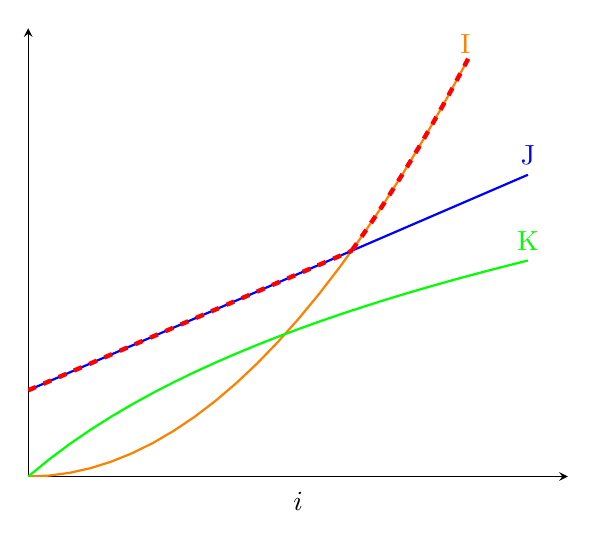
\begin{tikzpicture}
\begin{axis}[
    axis lines = left,
    xlabel = \(i\),
    ylabel = {},
    domain = 0:2.5,
    xtick={\empty},ytick={\empty},
    ymin=0,
    ymax=5.2,
    xmax=2.7,
    restrict y to domain=0:5,
]
    \addplot[thick, color=orange]{x^2} node[above,pos=1] {I};
    \addplot[thick, color=blue]{x+1} node[above,pos=1] {J};
    \addplot[thick, color=green]{ln(x+1)*2} node[above,pos=1] {K};
    \draw [ultra thick, dashed, draw=red] (axis cs:0,1) -- (axis cs:1.62,2.62);
    \addplot[ultra thick, color=green, dashed, color=red, domain=1.62:2.5]{x^2};
\end{axis}
\end{tikzpicture}
    \caption{Combined complexities illustrated. The combined complexity consists of the three indices I, J, K of the single index variable $i$. The dashed red line shows the bound of the combined complexity. $K$ is a superfluous index in the combined complexity as it never contributes to the bound of the combined complexity.}
    \label{fig:combined_complexity}
\end{figure}


\begin{defi}[Combined complexity]\label{def:combinedcomp} 
    We refer to a set $\kappa$ of complexities as a \textit{combined complexity}. We extend constraint judgements to include combined complexities such that
    \begin{enumerate}
        \item $\varphi;\Phi\vDash \kappa \leq \kappa'$ if for all $K \in \kappa$ there exists $K'\in \kappa'$ such that $\varphi;\Phi\vDash K \leq K'$.
        % 
        \item $\varphi;\Phi\vDash \kappa = \kappa'$ if $\varphi;\Phi\vDash \kappa \leq \kappa'$ and $\varphi;\Phi\vDash \kappa' \leq \kappa$.
        \item $\kappa + I = \{K + I \mid K \in \kappa\}$.
        %
        \item $\kappa\{J/i\} = \{ K\{J/i\} \mid K\in\kappa \}$.
    \end{enumerate}
    In the above, we may substitute an index for a combined complexity. In such judgements, the index represents a singleton set. For instance, $\varphi;\Phi\vDash \kappa \leq K$ represents $\varphi;\Phi\vDash \kappa \leq \{K\}$.
    %$\varphi;\Phi \vDash \kappa \bowtie \kappa' \quad\text{ if }\quad \forall K \in \kappa. (\exists K' \in \kappa'. \varphi;\Phi \vDash K \bowtie K')$.
\end{defi}

More specifically, when considering a combined complexity $\kappa$, we are interested in the maximal complexity given some valuation $\rho$, which we find by simply comparing the different values for the complexities within $\kappa$ given $\rho$. Note that the complexity $K \in \kappa$ that is maximal may be different for different valuations. In Definition \ref{def:combinedcomp} we extend the binary relations in $\bowtie$ on indices to combined complexities, such that we can compare two combined complexities such as $\varphi;\Phi \vDash \kappa \bowtie \kappa'$ and a combined complexity and complexity such as $\varphi;\Phi \vDash \kappa \bowtie K$. Definition \ref{def:combinedcompbasis} defines the function \textit{basis} that discards any $K \in \kappa$ that can never be the maximal complexity given some set of constraints $\Phi$ (i.e. the complexities that are bounded by other complexities in the set), such that we can always keep the number of complexities in a combined complexity to a minimum. %Finally, we may also be interested in adding an index onto a combined complexity, and so we define the addition of indices onto combined complexities in Definition \ref{def:combinedcompadd}.
%
\begin{defi}\label{def:combinedcompbasis}
    We define the function \textit{basis} that takes a set of index variables $\varphi$, a set of constraints $\Phi$ and a combined complexity $\kappa$, and returns a new combined complexity without superfluous complexities (The \textit{basis} of $\kappa$)
    \begin{align*}
        \text{basis}(\varphi,\Phi,\kappa) = \bigcap\left\{ \kappa' \subseteq \kappa \mid \forall K\in\kappa.\exists K'\in\kappa'.\varphi;\Phi\vDash K \leq K' \right\}
    \end{align*}
    Moreover, the algorithm below computes the basis
    % \begin{align*}
    %     \text{basis}(\varphi, \kappa) = \{(\Phi, K) \in \kappa \mid \varphi;\Phi \not \vDash K < K' \text{ for all } (\Phi', K') \in \kappa\}
    % \end{align*}
    \begin{align*}
        &\text{basis}(\varphi, \Phi, \kappa) = \text{do}\\[-0.5em]
        &\quad \kappa' \leftarrow \kappa\\[-0.5em]
        &\quad \text{for } K \in \kappa \text{ do}\\[-0.5em]
        &\quad\quad \text{ if } \exists K' \in \kappa' \text{ with } K \not = K' \text{ and } \varphi;\Phi \vDash K \leq K' \text{ then}\\[-0.5em]
        &\quad\quad\quad \kappa' \leftarrow \kappa' \setminus \{K\}\\[-0.5em]
        &\quad \text{return } \kappa'
    \end{align*}
\end{defi}
%
% \begin{defi}[]\label{def:combinedcompadd}
%     We define the the addition of a combined complexity and index as
%     \begin{align*}
%         \kappa + I = \{K + I \mid K \in \kappa\}
%     \end{align*}

% \end{defi}
%
For typing expressions, we use the rules presented in Table \ref{tab:sizedtypedexpressiontypes}, excluding the rule $\runa{BG-sub}$. In Table \ref{tab:sizedprocesstypingrules} we show the type rules for processes. Type judgements are of the form $\varphi;\Phi;\Gamma \vdash P \triangleleft \kappa$ where $\kappa$ denotes the complexity of process $P$. The rule $\runa{S-tick}$ types a \texttt{tick} prefix and incurs a cost of one in time complexity. We advance the time of all types in the context accordingly when typing the continuation. Rule $\runa{S-annot}$ is similar but may incur a cost of $n$. Matches on naturals are typed with rule $\runa{S-nmatch}$. Most notably, we extend the set of known constraints when typing the two continuations. That is, we can deduce constraints on the lower and upper bounds on the size of the expression we match on. For instance, for the zero pattern we can deduce that the lower bound $I$ must be equal to $0$ (or equivalently $I \leq 0$), and for the successor pattern, we can guarantee that the upper bound $J$ must be greater than or equal to $1$. For the complexity of pattern matches and parallel composition, we take advantage of the fact that we represent complexities using combined complexities. As such, we include complexities in both $P$ and $Q$ in the result. To remove redundancy from the set $\kappa \cup \kappa'$, we use the basis function.\\

%
% \begin{table*}[!ht]
%     \begin{framed}\vspace{-1em}\begin{align*}
%         &\kern15em\\[-2em] % Stretch frame
%         &\kern0em\runa{S-nil}\infrule{}{\varphi;\Phi;\Gamma \vdash \withcomplex{\nil}{0}} \kern1em\runa{S-tick}\;\infrule{\varphi;\Phi;\susumesim{\Gamma}{1}\vdash P \triangleleft K}{\varphi;\Phi;\Gamma\vdash \tick P \triangleleft K + 1} \kern3em\runa{S-nu}\;\infrule{\varphi;\Phi;\Gamma,\withtype{a}{T} \vdash \withcomplex{P}{K}}{\varphi;\Phi;\Gamma \vdash \newvar{a: T}{\withcomplex{P}{K}}}\\[-1em]
%         %
%         &\kern-0em\runa{S-nmatch}\;\condinfrule{
%         \begin{matrix}
%             \varphi;\Phi;\Gamma \vdash \withtype{e}{\natinterval{I}{J}}\quad \varphi;\Phi, I \leq 0;\Gamma \vdash \withcomplex{P}{K} \\
%             \varphi;\Phi, J \geq 1;\Gamma, \withtype{x}{\natinterval{I-1}{J-1}} \vdash \withcomplex{Q}{K'}
%         \end{matrix}}{\varphi;\Phi;\Gamma \vdash \withcomplex{\match{e}{P}{x}{Q}}{L}}{\text{where}\quad L = \left\{
% \begin{matrix}
%     K & \text{if}\; \varphi;\Phi\vDash K' \leq K   \\
%     K' & \text{if}\; \varphi;\Phi\vDash K \leq K'  \\
%     K+K' & \text{otherwise}
% \end{matrix}
% \right.}\\[-1em]
%         %
%         %&\kern-0em\runa{S-nmatch-2}\;\infrule{
%         %\begin{matrix}
%         %    \varphi;\Phi;\Gamma \vdash \withtype{e}{\natinterval{I}{J}} \quad \varphi;\Phi\vDash K \leq K' \\
%         %    \varphi;\Phi, I \leq 0;\Gamma \vdash \withcomplex{P}{K} \quad \varphi;\Phi, J \geq 1;\Gamma, \withtype{x}{\natinterval{I-1}{J-1}} \vdash \withcomplex{Q}{K'}
%         %\end{matrix}}{\varphi;\Phi;\Gamma \vdash \withcomplex{\match{e}{P}{x}{Q}}{K'}}\\[-1em]
%         %
%         &\kern-0em\runa{S-lmatch}\;\condinfrule{
%         \begin{matrix}
%             \varphi;\Phi;\Gamma \vdash \withtype{e}{\texttt{List}[I,J](\mathcal{B})} \quad \varphi;\Phi, I \leq 0;\Gamma \vdash \withcomplex{P}{K} \\
%             \varphi;\Phi, J \geq 1;\Gamma, \withtype{x}{\mathcal{B}},y : \texttt{List}[I-1,J-1](\mathcal{B}) \vdash \withcomplex{Q}{K'}
%         \end{matrix}}{\varphi;\Phi;\Gamma \vdash \withcomplex{\texttt{match}\;e\;\{ [] \mapsto P;\; x :: y \mapsto Q \}}{L}}{\text{where}\quad L = \left\{
% \begin{matrix}
%     K & \text{if}\; \varphi;\Phi\vDash K' \leq K   \\
%     K' & \text{if}\; \varphi;\Phi\vDash K \leq K'  \\
%     K+K' & \text{otherwise}
% \end{matrix}
% \right.}\\[-1em]
%         %
%         %&\kern-0em\runa{S-lmatch-2}\;\infrule{
%         %\begin{matrix}
%         %    \varphi;\Phi;\Gamma \vdash \withtype{e}{\texttt{List}[I,J](\mathcal{B})} \quad \varphi;\Phi\vDash K \leq K' \\
%         %    \varphi;\Phi, I \leq 0;\Gamma \vdash \withcomplex{P}{K} \quad \varphi;\Phi, J \geq 1;\Gamma, \withtype{x}{\mathcal{B}},y : \texttt{List}[I-1,J-1](\mathcal{B}) \vdash \withcomplex{Q}{K'}
%       % \end{matrix}}{\varphi;\Phi;\Gamma \vdash \withcomplex{\texttt{match}\;e\;\{ [] \mapsto P;\; x :: y \mapsto Q \}}{K'}}\\[-1em]
%         %
%         &\kern4em\runa{S-par}\;\condinfrule{\varphi;\Phi;\Gamma\vdash P \triangleleft K\quad \varphi;\Phi;\Gamma\vdash Q \triangleleft K'}{\varphi;\Phi;\Gamma\vdash \parcomp{P}{Q} \triangleleft L}{\text{where}\quad L = \left\{
% \begin{matrix}
%     K & \text{if}\; \varphi;\Phi\vDash K' \leq K   \\
%     K' & \text{if}\; \varphi;\Phi\vDash K \leq K'  %\\
%     %K+K' & \text{otherwise}
% \end{matrix}
% \right.}\\[-1em]
%         %
%         %&\kern4em\runa{S-par-2}\;\infrule{\varphi;\Phi;\Gamma\vdash P \triangleleft K\quad \varphi;\Phi;\Gamma\vdash Q \triangleleft K'\quad \varphi;\Phi\vDash K \leq K'}{\varphi;\Phi;\Gamma\vdash \parcomp{P}{Q} \triangleleft K'}\\[-1em]
%         %
%         &\kern-0em\runa{S-iserv}\;\infrule{\texttt{in}\in\sigma\quad \varphi,\widetilde{i};\Phi;\text{ready}(\varphi,\Phi,\susumesim{\Gamma}{I}),a:\forall_0\widetilde{i}.\texttt{serv}^{\sigma\cap\{\texttt{out}\}}_K(\widetilde{T}),\widetilde{v} : \widetilde{T}\vdash P \triangleleft K'\quad \varphi,\widetilde{i};\Phi\vDash K' \leq K}{\varphi;\Phi;\Gamma,a:\forall_I\widetilde{i}.\texttt{serv}^\sigma_K(\widetilde{T})\vdash\; \bang\inputch{a}{\widetilde{v}}{}{P}\triangleleft I}\\[-1em]
%         %
%         &\kern-0em\runa{S-ich}\;\infrule{\texttt{in}\in\sigma\quad \varphi;\Phi;\susumesim{\Gamma}{I},a:\texttt{ch}_0^\sigma(\widetilde{T}),\widetilde{v} : \widetilde{T}\vdash P \triangleleft K}{\varphi;\Phi;\Gamma,a:\texttt{ch}_I^\sigma(\widetilde{T})\vdash \inputch{a}{\widetilde{v}}{}{P}\triangleleft K + I}
%         %
%         \kern8.5em \runa{S-och}\;\infrule{\texttt{out}\in \sigma\quad \varphi;\Phi;\susumesim{\Gamma}{I}\vdash \widetilde{e} : \widetilde{T}\quad \varphi;\Phi\vdash\widetilde{T}\sqsubseteq\widetilde{S}}{\varphi;\Phi;\Gamma,a:\texttt{ch}^{\sigma}_I(\widetilde{S})\vdash \asyncoutputch{a}{\widetilde{e}}{} \triangleleft I}\\[-1em]
%         %
%         &\kern0em\runa{S-oserv}\;\infrule{\texttt{out} \in \sigma \quad \varphi;\Phi;\susumesim{\Gamma}{I}\vdash \widetilde{e} : \widetilde{T}\quad \text{instantiate}(\widetilde{i},\widetilde{T})=\{\widetilde{J}/\widetilde{i}\}\quad  \varphi;\Phi\vdash\widetilde{T}\sqsubseteq\widetilde{S}\{\widetilde{J}/\widetilde{i}\}}{\varphi;\Phi;\Gamma,a:\forall_I\widetilde{i}.\texttt{serv}_K^\sigma(\widetilde{S})\vdash \asyncoutputch{a}{\widetilde{e}}{} \triangleleft K\!\substi{\widetilde{J}}{\widetilde{i}} + I}
%         %
%     \end{align*}\vspace{-1em}\end{framed}
%     \smallskip
%     \caption{Sized typing rules for parallel complexity of processes.}
%     \label{tab:sizedprocesstypingrules}
% \end{table*}

\begin{table*}[!ht]
    \begin{framed}\vspace{-1em}\begin{align*}
        %
        % S-nil
        &\runa{S-nu}\infrule{\varphi;\Phi;\Gamma, a:T \vdash P \triangleleft \kappa}{\varphi;\Phi;\Gamma \vdash \newvar{a:T}{P} \triangleleft \kappa}
        % S-par
        \kern1em\runa{S-par}\infrule{\varphi;\Phi;\Gamma \vdash P \triangleleft \kappa \quad \varphi;\Phi;\Gamma \vdash Q \triangleleft \kappa'}{\varphi;\Phi;\Gamma \vdash P \mid Q \triangleleft \text{basis}(\varphi, \Phi,\kappa \cup \kappa')}\\[-1em]
        %
        &\runa{S-tick}\infrule{\varphi;\Phi;\tforwardsim{\Gamma}{1} \vdash P \triangleleft \kappa}{\varphi;\Phi;\Gamma \vdash \tick P \triangleleft \kappa + 1}\kern2em
        %
        \runa{S-annot}\infrule{\varphi;\Phi;\tforwardsim{\Gamma}{n}\vdash P \triangleleft \kappa}{\varphi;\Phi;\Gamma\vdash n:P \triangleleft \kappa + n}\\[-1em]
        % S-match
        &\runa{S-match}\infrule{
        \begin{matrix}
            \varphi;\Phi;\Gamma \vdash e:\natinterval{I}{J} \quad \varphi;\Phi, I \leq 0;\Gamma \vdash P \triangleleft \kappa\\
            \varphi;\Phi, J \geq 1;\Gamma, x:\natinterval{I-1}{J-1} \vdash Q \triangleleft \kappa'
        \end{matrix}}{\varphi;\Phi;\Gamma \vdash \match{e}{P}{x}{Q} \triangleleft \text{basis}(\varphi, \Phi, \kappa \cup \kappa')}\\[-1em]
        % S-iserv
        &\runa{S-iserv}\infrule{\begin{matrix}
            \texttt{in} \in \sigma\quad \varphi;\Phi;\Gamma\vdash a:\servt{I}{i}{\sigma}{K}{\widetilde{T}}\\
            \varphi, \widetilde{i}; \Phi; \text{ready}(\varphi,\Phi,\tforwardsim{\Gamma}{I}), \widetilde{v} : \widetilde{T} \vdash P \triangleleft \kappa \quad \varphi,\widetilde{i};\Phi\vDash\kappa \leq K
        \end{matrix}}
        {\varphi;\Phi;\Gamma \vdash \;\bang\inputch{a}{\widetilde{v}}{}{P}\triangleleft \{I\}}
        %
        \kern14em\runa{S-nil}\kern-1em\infrule{}{\varphi;\Phi;\Gamma \vdash \nil \triangleleft \{0\}}\kern-3em\text{ }\\[-1em]
        % S-oserv
        &\runa{S-oserv}\infrule{\begin{matrix}
            \texttt{out} \in \sigma\quad \varphi;\Phi;\Gamma\vdash a:\servt{I}{i}{\sigma}{K}{\widetilde{T}}\\
            \varphi; \Phi;\tforwardsim{\Gamma}{I} \vdash \widetilde{e}:\widetilde{S} \quad \text{instantiate}(\widetilde{i}, \widetilde{S}) = \{\widetilde{J}/\widetilde{i}\} \quad \varphi;\Phi \vDash \widetilde{S} \sqsubseteq \widetilde{T}
        \end{matrix}}
        {\varphi;\Phi;\Gamma \vdash \asyncoutputch{a}{\widetilde{e}}{}\triangleleft \{K\{\widetilde{J}/\widetilde{i}\} + I\}}\\[-1em]
        % S-annot
        &\runa{S-ich}\infrule{\begin{matrix}
            \texttt{in} \in \sigma\quad \varphi;\Phi;\Gamma \vdash a:\chant{\sigma}{I}{\widetilde{T}}\\
            \varphi; \Phi; \tforwardsim{\Gamma}{I}, \widetilde{v}:\widetilde{T} \vdash P \triangleleft \kappa
        \end{matrix}}
        {\varphi;\Phi;\Gamma \vdash \inputch{a}{\widetilde{v}}{}{P} \triangleleft \kappa + I}\kern3em
        %
        \runa{S-och}\infrule{\begin{matrix}
            \texttt{out} \in \sigma\quad \varphi;\Phi;\Gamma \vdash a:\chant{\sigma}{I}{\widetilde{T}}\\
            \varphi; \Phi; \tforwardsim{\Gamma}{I} \vdash \widetilde{e}:\widetilde{S} \quad \varphi;\Phi \vDash \widetilde{S} \sqsubseteq \widetilde{T}
        \end{matrix}}
        {\varphi;\Phi;\Gamma \vdash \asyncoutputch{a}{\widetilde{e}}{} \triangleleft \{I\}}\\[-1em]
    \end{align*}\vspace{-1em}\end{framed}
    \smallskip
    \caption{Sized typing rules for parallel complexity of processes.}
    \label{tab:sizedprocesstypingrules}
\end{table*}

%
Rule $\runa{S-iserv}$ types a replicated input on a name $a$, and so $a$ must be bound to a server type with input capability. As the index $I$ in the server type denotes the time steps remaining before the server is ready to synchronize, we advance the time by $I$ units of time complexity when typing the continuation $P$. To ensure that bounds on synchronizations in $\downarrow^{\varphi;\Phi}_I\!\Gamma$ are not violated, we type $P$ under the time invariant part of $\downarrow^{\varphi;\Phi}_I\!\Gamma$, i.e. $\text{ready}(\varphi,\Phi,\downarrow_I\!\Gamma)$. Note that the bound on the span of the replicated input is the bound on the time remaining before the server is ready to synchronize. As the replicated input may be invoked many times, the cost of invoking the server is accounted for in rule $\runa{S-oserv}$ using the complexity bound $K$ in the server type. Therefore, we enforce that $K$ is in fact an upper bound on the span of the continuation $P$.\\

The rule $\runa{S-oserv}$ types outputs on names bound to server types. Here, as stated above, we must account for the cost of invoking a server, and as a replicated input on a server is parametric, we must \textit{instantiate} it based on the types of the expressions we are to output. Recall that in the type rule for outputs on servers from Chapter \ref{ch:bgts}, this is to be done by finding a substitution that satisfies the premise $\widetilde{T} \sqsubseteq \widetilde{S}\{\widetilde{J}/\widetilde{i}\}$. However, this turns out to be a difficult problem, and we can in fact prove it NP-complete for types of polynomial indices even if we disregard subtyping. However, note that it might not be necessary to use the full expressive power of polynomial indices, and so this may not necessarily affect type checking. Nevertheless, we over-approximate finding such a substitution, by using the function $\textit{instantiate}$. That is, we \textit{zip} together the index variables $\widetilde{i}$ with indices in types $\widetilde{T}$. Remark that Baillot and Ghyselen \cite{BaillotGhyselen2021} propose types for inference in their technical report, where the problem is simplified substantially, by forcing naturals to have lower bounds of $0$ and upper bounds with exactly one index variable and a constant. Our approach admits more expressive lower bounds and multiplications, while imposing no direct restrictions on the number of index variables in an index, and is thus more suitable for a type-checker.\\

We now prove the NP-completeness of the smaller problem of checking whether there exists a substitution $\{\widetilde{J}/\widetilde{i}\}$ that satisfies $T = S\{\widetilde{J}/\widetilde{i}\}$ where $T$ and $S$ are types with polynomial indices. The main idea is a reduction proof from the NP-complete 3-SAT problem, i.e. the satisfiability problem of a boolean formula in conjunctive normal form with exactly three literals in each clause \cite{Karp1972}. We first define a translation from a 3-SAT formula to a polynomial index in Definition \ref{def:3satredu}. This is a polynomial time computable reduction, as we simply replace each logical-and with a multiplication, each logical-or with an addition and each negation with a subtraction from 1. In Lemma \ref{lemma:soundtranslation}, we prove that the reduction is faithful with respect to satisfiability of a boolean formula. Finally, in Lemma \ref{lemma:npcompletesubst}, we prove that it is an NP-complete decision problem to verify the existence of a substitution that satisfies $T = S\{\widetilde{J}/\widetilde{i}\}$ for types $T$ and $S$.
%
\begin{defi}[3-SAT reduction]\label{def:3satredu}
We assume a one-to-one mapping $f$ from unknowns to index variables. Let $\phi$ be a 3-SAT formula
\begin{align*}
    \phi = \bigwedge_{i=1}^n \left(\ell_{i1} \lor \ell_{i2} \lor \ell_{i3}\right)% \land \cdots \land (A_n \lor B_n \lor C_n)
\end{align*}
where $\ell_{i1}$, $\ell_{i2}$ and $\ell_{i3}$ are of the forms $x$ or $\neg x$ for some variable $x$. We define a translation of $\phi$ to a polynomial index %$[\![\phi]\!]_{\text{3-SAT}}$
\begin{align*}
    [\![\phi]\!]_{\text{3-SAT}} = \prod_{i=1}^n \left([\![\ell_{i1}]\!]_{\text{3-SAT}} + [\![\ell_{i2}]\!]_{\text{3-SAT}} + [\![\ell_{i3}]\!]_{\text{3-SAT}}\right) %\cdots ([\![A_n]\!]_{\text{3-SAT}} + [\![B_n]\!]_{\text{3-SAT}} + [\![C_n]\!]_{\text{3-SAT}})
\end{align*}
where $[\![x]\!]_{\text{3-SAT}} = f(x)$ and $[\![\neg x]\!]_{\text{3-SAT}} = (1 - f(x))$.
\end{defi}


\begin{lemma}\label{lemma:soundtranslation}
Let $\phi$ be a 3-SAT formula. Then $\phi$ is satisfiable if and only if there exists a substitution $\{\widetilde{n}/\widetilde{i}\}$ such that $1\leq [\![\phi]\!]_{\text{3-SAT}}\{\widetilde{n}/\widetilde{i}\}$.
\begin{proof}
We consider the implications separately
\begin{enumerate}
    \item Assume that $\phi$ is satisfiable. Then there exists a truth assignment $\tau$ such that each clause of $\phi$ is true. Correspondingly, as $[\![\phi]\!]_{\text{3-SAT}}$ is a product of non-negative factors, we for some substitution $\{\widetilde{n}/\widetilde{i}\}$ have that $1 \leq [\![\phi]\!]_{\text{3-SAT}}\{\widetilde{n}/\widetilde{i}\}$ if and only if each factor in the product is positive. We compare the conditions for a clause to be true in $\phi$ to those for a corresponding factor in $[\![\phi]\!]_{\text{3-SAT}}$ to be positive, and show that a substitution $\{\widetilde{n}/\widetilde{i}\}$ exists such that $1 \leq [\![\phi]\!]_{\text{3-SAT}}\{\widetilde{n}/\widetilde{i}\}$. A clause in $\phi$ is a disjunction of three literals of either the form $x$ or $\neg x$ for some unknown $x$. Thus, for a clause to be true, we must have at least one literal $\tau(x) = tt$ or $\neg \tau(x) = tt$ with $\tau(x) = f\!f$. The corresponding factor in $[\![\phi]\!]_{\text{3-SAT}}$ is a sum of three terms of the forms $f(x)$ or $(1 - f(x))$ for some unknown $x$, where $f$ is a one-to-one mapping from unknowns to index variables. Here, we utilize that in the type system by Baillot and Ghyselen \cite{BaillotGhyselen2021}, we have $(1 - i\{\widetilde{n}/\widetilde{i}\}) = 0$ when $i\{\widetilde{n}/\widetilde{i}\} \geq 1$ and $(1 - i\{\widetilde{n}/\widetilde{i}\}) = 1$ when $i\{\widetilde{n}/\widetilde{i}\} = 0$. Thus, for a factor to be positive, it suffices that one term is positive, and so we can construct a substitution that guarantees this from the interpretation of $\phi$. That is, if $\tau(x) = tt$, we substitute $1$ for $f(x)$, and if $\tau(x) = f\!f$, we substitute 0 for $f(x)$. Then, whenever a literal is true in $\phi$, the corresponding term in $[\![\phi]\!]_{\text{3-SAT}}$ is positive, and so if $\phi$ is satisfiable then there exists a substitution $\{\widetilde{n}/\widetilde{i}\}$ such that $1 \leq [\![\phi]\!]_{\text{3-SAT}}\{\widetilde{n}/\widetilde{i}\}$.
     
    \item Assume that there exists a substitution $\{\widetilde{n}/\widetilde{i}\}$ such that $1 \leq [\![\phi]\!]_{\text{3-SAT}}\{\widetilde{n}/\widetilde{i}\}$. Then, as $[\![\phi]\!]_{\text{3-SAT}}$ is a product of non-negative factors, each factor must be positive. Correspondingly, if $\Phi$ is satisfiable, then there exists a truth assignment such that each clause of $\phi$ is true. We compare the conditions for a factor in $[\![\phi]\!]_{\text{3-SAT}}\{\widetilde{n}/\widetilde{i}\}$ to be positive to those for a corresponding clause in $\phi$ to be true, and show that $\phi$ is satisfiable. A factor in $[\![\phi]\!]_{\text{3-SAT}}$ is a sum of at most three terms of the forms $f(x)\{\widetilde{n}/\widetilde{i}\}$ or $(1 - f(x)\{\widetilde{n}/\widetilde{i}\})$. Here we again utilize that in the type system by Baillot and Ghyselen \cite{BaillotGhyselen2021}, we have $(1 - f(x)\{\widetilde{n}/\widetilde{i}\}) = 0$ when $f(x)\{\widetilde{n}/\widetilde{i}\} \geq 1$ and $(1 - f(x)\{\widetilde{n}/\widetilde{i}\}) = 1$ when $f(x)\{\widetilde{n}/\widetilde{i}\} = 0$, and so it must be that in the factor, we have at least one term $f(x)\{\widetilde{n}/\widetilde{i}\} \geq 1$ or $(1 - f(x)\{\widetilde{n}/\widetilde{i}\}) \geq 1$. Correspondingly, for the clause in $\phi$ to be true, at least one literal must be true. We show that there exists a truth assignment $\tau$ such that if a term in $[\![\phi]\!]_{\text{3-SAT}}$ is positive, then the corresponding literal in $\phi$ is true. If $f(x)\{\widetilde{n}/\widetilde{i}\}\geq 1$ then we set $\tau(x) = tt$, and if $f(x)\{\widetilde{n}/\widetilde{i}\} = 0$ we set $\tau(x) = f\!f$, as $[\![x]\!]_{\text{3-SAT}}\{\widetilde{n}/\widetilde{i}\} \geq 1$ when $f(x)\{\widetilde{n}/\widetilde{i}\} \geq 1$ and $[\![\neg x]\!]_{\text{3-SAT}} \geq 1$ when $f(x)\{\widetilde{n}/\widetilde{i}\}=0$. Then, whenever a term is positive in $[\![\phi]\!]_{\text{3-SAT}}\{\widetilde{n}/\widetilde{i}\}$, the corresponding literal in $\phi$ is true, and so if there exists a substitution $\{\widetilde{n}/\widetilde{i}\}$ such that $1 \leq [\![\phi]\!]_{\text{3-SAT}}\{\widetilde{n}/\widetilde{i}\}$, then $\phi$ is satisfiable.
    
\end{enumerate}
\end{proof}
\end{lemma}


\begin{lemma}\label{lemma:npcompletesubst}
Let $T$ and $S$ be types with polynomial indices. Then checking whether there exists a substitution $\{\widetilde{J}/\widetilde{i}\}$ such that $T = S\{\widetilde{J}/\widetilde{i}\}$ is an NP-complete problem.
\begin{proof}
By reduction from the 3-SAT problem. Assume that we have some algorithm that can verify the existence of a substitution $\{\widetilde{J}/\widetilde{i}\}$ such that $T = S\{\widetilde{J}/\widetilde{i}\}$, and let $\phi$ be a 3-SAT formula. Then using the algorithm, we can check whether $\phi$ is satisfiable by verifying whether there exists $\{\widetilde{J}/\widetilde{i}\}$ such that the following holds
\begin{align*}
    \texttt{Nat}[0,1] = \texttt{Nat}[0,(1 - (1 - [\![\phi]\!]_{\text{3-SAT}}))]\{\widetilde{J}/\widetilde{i}\}
\end{align*}
That is, $1 = (1 - (1 - [\![\phi]\!]_{\text{3-SAT}}\{\widetilde{J}/\widetilde{i}\}))$ implies $1 \leq [\![\phi]\!]_{\text{3-SAT}}\{\widetilde{J}/\widetilde{i}\}$, as $(1 - [\![\phi]\!]_{\text{3-SAT}}\{\widetilde{J}/\widetilde{i}\}) = 0$ when $[\![\phi]\!]_{\text{3-SAT}}\{\widetilde{J}/\widetilde{i}\} \geq 1$ and $(1 - [\![\phi]\!]_{\text{3-SAT}}\{\widetilde{J}/\widetilde{i}\}) = 1$ when $[\![\phi]\!]_{\text{3-SAT}}\{\widetilde{J}/\widetilde{i}\} = 0$. Furthermore, for $1 \leq [\![\phi]\!]_{\text{3-SAT}}\{\widetilde{J}/\widetilde{i}\}$ to hold, the indices in the sequence $\widetilde{J}$ cannot contain index variables, and so there must exist an equivalent substitution of naturals for index variables $\{\widetilde{n}/\widetilde{i}\}$. Then, by Lemma \ref{lemma:soundtranslation} we have that $\phi$ is satisfiable if and only if there exists a substitution $\{\widetilde{n}/\widetilde{i}\}$ such that $1\leq [\![\phi]\!]_{\text{3-SAT}}\{\widetilde{n}/\widetilde{i}\}$. Thus, as 3-SAT is an NP-complete problem, the reduction from 3-SAT is computable in polynomial time and as polynomial reduction is a transitive relation, i.e. any NP-problem is polynomial time reducible to verifying the existence of a substitution $\{\widetilde{J}/\widetilde{i}\}$ that satisfies the equation $T = S\{\widetilde{J}/\widetilde{i}\}$, it follows that the problem is NP-hard. To show that it is an NP-complete problem, we show that a \textit{certificate} can be verified in polynomial time. That is, given some substitution $\{\widetilde{J}/\widetilde{i}\}$, we can in linear time check whether $T=S\{\widetilde{J}/\widetilde{i}\}$ by substituting indices $\widetilde{J}$ for indices $\widetilde{i}$ in type $S$ and by then comparing the two types.\\
%
%
%Utilizing that $n - m = 0$ for $m\geq n$ in the type system of Baillot and Ghyselen \cite{BaillotGhyselen2021}, we can simulate any boolean formula using a polynomial index. By denoting $J = 0$ false and $I > 0$ true, we have the translation
% \begin{align*}
%     [\![a \land b]\!]_\phi =&\; [\![a]\!]_\phi [\![b]\!]_\phi\\
%     [\![a \lor b]\!]_\phi =&\; [\![a]\!]_\phi + [\![b]\!]_\phi\\
%     [\![\neg a]\!]_\phi =&\; (1 - [\![a]\!]_\phi)\\
%     [\![x]\!]_\phi =&\; i
% \end{align*}
% Then assuming some algorithm that checks whether there exists a substitution $\{\widetilde{J}/\widetilde{i}\}$ such that $T \sqsubseteq S\{\widetilde{J}/\widetilde{i}\}$, we can solve the boolean satisfiability problem. Let $\phi_0$ be any boolean formula and let $\widetilde{i}$ be the index variables in $[\![\phi_0]\!]_\phi$, and assume that there exists a substitution $\{\widetilde{J}/\widetilde{i}\}$ that satisfies the judgement
% \begin{align*}
%     \emptyset;\emptyset\vDash\texttt{Nat}[0,1] \sqsubseteq \texttt{Nat}[0,[\![\phi_0]\!]_\phi]\{\widetilde{J}/\widetilde{i}\}
% \end{align*}
% Then by rule $\runa{SS-nweak}$ we have that $\emptyset;\emptyset\vDash 1 \leq [\![\phi_0]\!]_\phi\{\widetilde{J}/\widetilde{i}\}$, and as $\varphi = \emptyset$, the indices $\widetilde{J}$ must be constants. Thus, $\emptyset;\emptyset\vDash 1 \leq [\![\phi_0]\!]_\phi\{\widetilde{J}/\widetilde{i}\}$ is equivalent to $1 \leq [\![\phi_0]\!]_\phi\{\widetilde{J}/\widetilde{i}\}$, and so $\phi_0$ must have a solution. If instead no such substitution exists, then for any $\{\widetilde{J}/\widetilde{i}\}$, it must be that $[\![\phi_0]\!]_\phi\{\widetilde{J}/\widetilde{i}\} = 0$ implying that $\phi_0$ is a contradiction. Therefore, as the boolean satisfiability problem is NP-complete, the algorithm we assumed must be NP-complete as well.
\end{proof}
\end{lemma}

In Example \ref{example:addition}, we show how a process implementing addition of naturals can be typed using our type rules, yielding a precise bound on the parallel complexity.
%

\begin{examp}\label{example:addition}
As an example of a process that is typable using our type rules, we show how the addition operator for naturals can be written as a process and subsequently be typed. We use a server to encode the addition operator
\begin{align*}
    !\inputch{\text{add}}{x,y,r}{}{\match{x}{\asyncoutputch{r}{y}{}}{z}{\tick{\asyncoutputch{\text{add}}{z,\succc y,r}{}}}}
\end{align*}
such that channel $r$ is used to output the addition of naturals $x$ and $y$. To type the process, we use the following contexts and set of index variables
\begin{align*}
    \Gamma\defeq&\; \text{add} : \forall_0 i,j,k,l,m,n,o.\texttt{serv}^{\{\texttt{in},\texttt{out}\}}_j(\texttt{Nat}[0,j],\texttt{Nat}[0,l],\texttt{ch}^{\{\texttt{out}\}}_j(\texttt{Nat}[0,j+l])) \\
    \Delta\defeq&\; \text{ready}(\cdot,\cdot,\Gamma), x : \texttt{Nat}[0,j], y: \texttt{Nat}[0,l], r:\texttt{ch}^{\{\texttt{out}\}}_j(\texttt{Nat}[0,j+l])\\
    \varphi \defeq&\; \{i,j,k,l,m,n,o\}
\end{align*}
%
We now derive a type for the encoding of the addition operator, yielding a precise bound of $j$, corresponding to an upper bound on the size of $x$, as we pattern match at most $j$ times on natural $x$. Notably we have that $\text{instantiate}((i,j,k,l,m,n,o),\texttt{Nat}[0,j\monus 1],\texttt{Nat}[1,l+1],\texttt{ch}^{\{\texttt{out}\}}_j(\texttt{Nat}[0,j+l]))=\{0/i,j\monus 1/j,0/k,l+1/l,j/m,0/n,j+l/o\}$.
%
{\small
\begin{align*}
    \begin{prooftree}
        %
        \infer0{\varphi;\cdot,0\leq 0;\Delta\vdash \asyncoutputch{r}{y}{} \triangleleft \{j\}}
        %
        % \infer0{\texttt{Nat}[0,j\monus 1] \sqsubseteq \texttt{Nat}[0,j]\{j\monus 1/j\}}
        % %
        % \infer0{\texttt{Nat}[0,l+1] \sqsubseteq \texttt{Nat}[0,l]\{l+1/l\}}
        % %
        % \infer0{\texttt{ch}^{\{\texttt{out}\}}_{j\monus 1}(\texttt{Nat}[0,j+l] \sqsubseteq \texttt{ch}^{\{\texttt{out}\}}_{j\monus 1}(\texttt{Nat}[0,j+l)\{j\monus 1/j,l+1/l\}}
        %
        \infer0{
        \begin{matrix}
        \varphi;\cdot,1\leq j\vdash\texttt{Nat}[0,j\monus 1] \sqsubseteq \texttt{Nat}[0,j]\{j\monus 1/j\}\\
        \varphi;\cdot,1\leq j\vdash\texttt{Nat}[1,l+1] \sqsubseteq \texttt{Nat}[0,l]\{l+1/l\}\\
        \varphi;\cdot,1\leq j\vdash\texttt{ch}^{\{\texttt{out}\}}_{j\monus 1}(\texttt{Nat}[0,j+l] \sqsubseteq \texttt{ch}^{\{\texttt{out}\}}_{j\monus 1}(\texttt{Nat}[0,j+l)\{j\monus 1/j,l+1/l\}
        \end{matrix}
        }
        %
        \infer1{\varphi;\cdot,1\leq j;\susumesim{\Delta}{1},z : \texttt{Nat}[0,j\monus 1]\vdash \asyncoutputch{\text{add}}{z,\succc y, r}{} \triangleleft \{j\monus 1\}}
        %
        \infer1{\varphi;\cdot,1\leq j;\Delta,z : \texttt{Nat}[0,j\monus 1]\vdash \tick{\asyncoutputch{\text{add}}{z,\succc y, r}{}} \triangleleft \{j\}}
        %
        \infer2{\varphi;\cdot;\Delta\vdash \match{x}{\asyncoutputch{r}{y}{}}{z}{\tick{\asyncoutputch{\text{add}}{z,\succc y,r}{}}} \triangleleft \{j\}}
        %
        \infer1{\cdot;\cdot;\Gamma\vdash\; !\inputch{\text{add}}{x,y,r}{}{\match{x}{\asyncoutputch{r}{y}{}}{z}{\tick{\asyncoutputch{\text{add}}{z,\succc y,r}{}}}}\triangleleft \{0\}}
    \end{prooftree}
\end{align*}}
%
\end{examp}

% \subsection{Undecidability of judgements}
% Verifying whether a polynomial constraint with integer coefficients imposes further restrictions onto the model set of index valuations of natural codomain of some set of known constraints can be reduced to Hilbert's tenth problem \cite{Davis1973}. That is, the problem of verifying whether a diophantine equation has an integer solution.\\

% We first assume some algorithm that can verify a judgement of the form $\varphi;\Phi\vDash C$ where $\varphi$ is a set of index variables and $C$ and $C'\in\Phi$ are binary constraints on polynomials of integer coefficients over relations from any subset of $\{\neq,\leq, <\}$. Recall that such a judgement holds exactly when for each index valuation $\rho : \varphi \longrightarrow \mathbb{N}$ over $\varphi$ for which $\rho \vDash C'$ for $C'\in\Phi$ we also have $\rho\vDash C$, i.e. $C$ does not impose further restrictions on interpretations of indices.\\

% We can then verify whether any diophantine equation has an integer solution. Let $p$ be an arbitrary polynomial of integer coefficients such that $p = 0$ is a diophantine equation. As only non-negative integers substitute for index variables, we first transform $p = 0$ to a new diophantine equation $p' = 0$ that has a non-negative integer solution exactly when $p = 0$ has an integer solution. To do this, we simply replace each index variable $i$ in $p$ with two new index variables $i_1 - i_2$. Then the judgement $\varphi;\emptyset\vDash p' \neq 0$ holds exactly when $p=0$ has no integer solution. That is, if $p=0$ has an integer solution, then there must exist a valuation $\rho_0$ such that $\rho_0\vDash \emptyset$ with $[\![p']\!]_{\rho_0} = 0$ and so $\rho_0\nvDash p' \neq 0$. Moreover, we need not rely on the relation $\neq$, as the judgements below are equivalent
% \begin{align*}
%     \varphi;\{p' \leq 0\} \vDash p' < 0\\
%     \varphi;\{p' \leq 0\} \vDash p' \leq 1
% \end{align*}

\subsection{Soundness}\label{sec:tcsoundness}
In this section, we prove the soundness of the type system presented in Section \ref{section:typeruless}. That is, we prove a subject reduction result and that a typing of a process provides a bound on the parallel complexity of the process. We first augment the definition of annotated processes and extend the type rules.
%
\subsection{Augmented language and type system}
In the type system from Chapter \ref{ch:bgts}, subtyping rules for processes and expressions are used extensively to bound parallel compositions and to prove a subject reduction property. However, such use of subtyping is notoriously difficult to implement, as there may be an infinite number of subtypes. Consider for instance a parallel composition of two processes $P$ and $Q$ that are typed as $\varphi;\Phi;\Gamma\vdash P \triangleleft 10 - i$ and $\varphi;\Phi;\Gamma\vdash Q \triangleleft i^2 - 100i$, respectively. These complexities are both functions of $i$ and clearly intersect. It is not trivial to find a common subtype of these indices in practice, and for more complex indices, it quickly becomes intractable.\\

In the case of subject reduction, where we have a reduction $P \Longrightarrow Q$, Baillot and Ghyselen \cite{BaillotGhyselen2021} use a subtyping rule for expressions extensively. In particular, upon synchronization of an input and an output on some channel, we require that the expressions to be transmitted can be typed as super types of the message types of the channel. Thus, upon reduction we use the subtyping rule to assign the message types to the expressions. In this case, we use information from the typing of $P$ to \textit{guide} subtyping in the typing of $Q$, and so by augmenting the reduction relation with annotations, we can implement subtyping. An alternative is to permit the subtyping rule for expressions to prove the soundness of the type system, and then omit it from the implementation, i.e. we simply reject processes that cannot be typed without using the subtyping rule. This is a valid compromise, as it avoids needless cluttering of the reduction relation with annotations, and we are usually not interested in using the subject reduction property in practice. That is, we need only type a process prior to any reduction, presuming the type system is sound. Therefore, we take this approach, introducing the subtyping rule for expressions below.
\begin{align*}
    \runa{S-subsumption}\;\infrule{\varphi;\Phi;\Gamma\vdash e : S\quad \varphi;\Phi\vdash S \sqsubseteq T}{\varphi;\Phi;\Gamma\vdash e : T}
\end{align*}
As reduction may reduce ticks, subsequently modifying the typing of a process, we need a \textit{delaying} property to prove a subject reduction result. That is, it must be safe to increase the bound in a typing, so long as all bounds on synchronizations in the type context are correspondingly increased (We write this as $\uparrow^I\!\!\Gamma$ when we increase bounds by $I$, as defined in Definition \ref{def:delayy}). Such a property is proved by induction on the type rules.
%
\begin{definition}[Delaying]\label{def:delayy}
We define the delaying $\uparrow^I\!\!T$ of a type $T$ by an index $I$ by the rules 
\begin{align*}
    \uparrow^L\!\!\texttt{Nat}[I,J] =&\; \texttt{Nat}[I,J]\\
    \uparrow^L\!\!\texttt{ch}^\sigma_I(\widetilde{T}) =&\; \texttt{ch}^\sigma_{I+L}(\widetilde{T})\\
    \uparrow^L\!\!\forall_I\widetilde{i}.\texttt{serv}^\sigma_K(\widetilde{T}) =&\; \forall_{I+L}\widetilde{i}.\texttt{serv}^\sigma_K(\widetilde{T})
\end{align*}
We extend delaying to contexts such that for all $v\in\texttt{dom}(\Gamma)$ such that $\Gamma(v)=T$ we have that $(\uparrow^I\!\!\Gamma)(v)=\uparrow^I\!\!T$.
\end{definition}
%
However, this turns out to be problematic due to type annotations on restrictions. That is, in the clause for restriction, we can assume that $\varphi;\Phi;\Gamma\vdash (\nu a :T) P \triangleleft \kappa$ from which we also have $\varphi;\Phi;\Gamma,a:T\vdash P \triangleleft \kappa$, and by induction we obtain $\varphi;\Phi;\uparrow^I\!\!\Gamma,a:\uparrow^I\!\!T\vdash P \triangleleft \kappa + I$, which unfortunately does not comply with the type annotation in $(\nu a:T) P$. Without a delaying property, we are (to our knowledge) unable to preserve a typing upon reduction, i.e. either the needed type context or assignable combined complexity (possibly both) changes. Unfortunately, this is an insufficient condition to prove that a bound on an assigned combined complexity $\kappa$ is in fact a bound on the span, as constant changes to expressions $I$ or $J$ in a judgement $\varphi;\Phi;\Gamma\vdash I \bowtie J$ is enough to sometimes (even for linear functions) fail a judgement. An example of this is depicted in Figure \ref{fig:srnecess}, showcasing that a strong subject reduction property is crucial to prove soundness.\\ %Consider for instance the two univariate linear functions below\\

\begin{figure}
    \centering
  %  \begin{minipage}{.5\textwidth}
    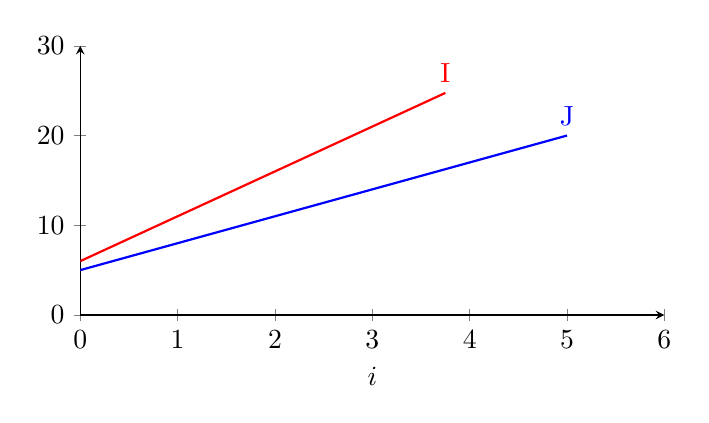
\begin{tikzpicture}
        \begin{axis}[
            axis lines = left,
            xlabel = \(i\),
            ylabel = {},
            domain = 0:5,
            xmin=0,
            xmax=6,
            ymin=0,
            ymax=30,
            restrict y to domain=0:25,
            height=5cm,
            width=9cm,
        ]
        \addplot[thick, color=red]{5*x+6} node[above,pos=1] {I};
        \addplot[thick, color=blue]{3*x+5} node[above,pos=1] {J};
    \end{axis}
    \end{tikzpicture}
\end{minipage}%
\begin{minipage}{.5\textwidth}
    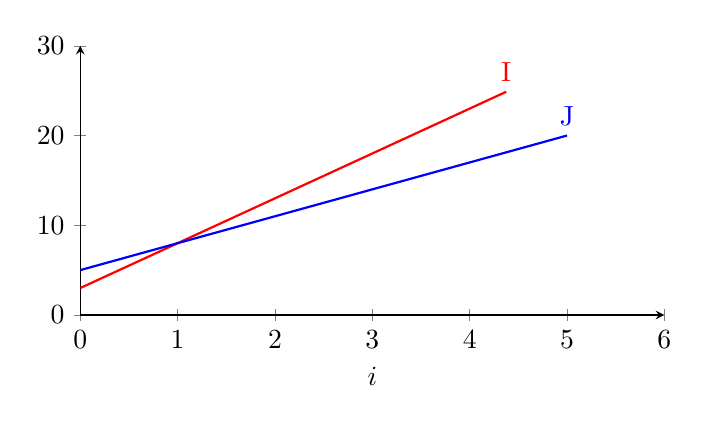
\begin{tikzpicture}
        \begin{axis}[
            axis lines = left,
            xlabel = \(i\),
            ylabel = {},
            domain = 0:5,
            xmin=0,
            xmax=6,
            ymin=0,
            ymax=30,
            restrict y to domain=0:25,
            height=5cm,
            width=9cm,
        ]
        \addplot[thick, color=red]{5*x+3} node[above,pos=1] {I};
        \addplot[thick, color=blue]{3*x+5} node[above,pos=1] {J};
    \end{axis}
    \end{tikzpicture}
\end{minipage}
%[width=5cm]%
    \caption{The image on the left depicts two linear indices $I = 5i+6$ and $J= 3i+5$ as functions of $i$ that do not intersect in the non-negative valuation space of $i$. On the right, we subtract $3$ from $I$, shifting the intersection of $I$ and $J$ into the non-negative valuation space. Thus, $\{i\};\cdot\vDash J \leq I$ but $\{i\};\cdot\nvDash J \leq I-3$. }
    \label{fig:srnecess}
\end{figure}
%
%\includegraphics[width=13cm]{image.png}\\
%Subtracting $3$ from $f$ is enough to shift the intersection of $f$ and $g$ into the non-negative valuation space. Thus, to prove the soundness of an implementation of the type system, it is crucial to have a strong subject reduction property.\\

As we are not interested in actually using a subject reduction property in practice, we can introduce two versions of the implementation: One with type annotations on restrictions, and one without. That is, one without a subject reduction property, and one with a subject reduction property. Intuitively, if $\varphi;\Phi;\Gamma\vdash P \triangleleft \kappa$ by the type system with annotations, then also $\varphi;\Phi;\Gamma\vdash P \triangleleft \kappa$ by the type system without annotations, and so it suffices to prove soundness for the type system without type annotations, to show that any bound on $\kappa$ is an upper bound on the span. Thus, in the remainder of this section, we assume that restrictions do not have type annotations.

%As our restrictions have type annotations, and as annotations advance the time of a context, the structural congruence definition must be augmented to prove a subject congruence result. Consider for instance the process $n : \newvar{a : \texttt{ch}^\sigma_I(\widetilde{T})}{\inputch{a}{\widetilde{v}}{}{P}}$ with some typing $\varphi;\Phi;\Gamma\vdash n : \newvar{a : \texttt{ch}^\sigma_I(\widetilde{T})}{\inputch{a}{\widetilde{v}}{}{P}} \triangleleft \kappa + I + n$ with $\varphi;\Phi;\downarrow_n\!\!\Gamma,a:\texttt{ch}^\sigma_I(\widetilde{T})\vdash \inputch{a}{\widetilde{v}}{}{P} \triangleleft \kappa + I$. Then $\newvar{a : \texttt{ch}^\sigma_I(\widetilde{T})}{n : \inputch{a}{\widetilde{v}}{}{P}}$ is not typable whenever $\varphi;\Phi\nvDash n\leq I$. However, we can quickly verify that $\varphi;\Phi;\Gamma\vdash \newvar{a : \texttt{ch}^\sigma_{I+n}(\widetilde{T})}{n : \inputch{a}{\widetilde{v}}{}{P}} \triangleleft \kappa + I + n$. Thus, if we \textit{delay} or advance the time of a type annotation upon a time annotation in and out (respectively) of the scope of the corresponding restriction, then the subject congruence property holds. Therefore, we formalize \textit{delaying} of types in Definition \ref{def:delayy}. 
%
%if intuitively $\varphi;\Phi;\Gamma,a:\text{delay}(\varphi,\Phi,\Gamma,\iota)\vdash \iota : P \triangleleft K$ where $I$ is the advancement of time imposed by $\iota$.
%

%
% We augment the structural congruence rule $\runa{SC-ares}$ correspondingly
% \begin{align*}
%     \runa{SC-ares}\; n : \newvar{a:T}{P} \equiv \newvar{a:T^{+n}}{n : P}
% \end{align*}
% %
% Moreover, we assume the subsequent rules for restrictions are extended with type annotations. Note that the changes to $\runa{SC-ares}$ do not affect the existence of a canonical form, as we can always apply $\runa{SC-ares}$ from left to right (As we do in the proof of Lemma \ref{lemma:anncannform}), as $T^{+n}$ is defined for any $n$ whenever $T$ is defined.
% %
% % \begin{align*}
%     \text{delay}(\varphi,\Phi,\Gamma,\epsilon, T) =&\; T \\
%     %
%     \text{delay}(\varphi,\Phi,\Gamma,(1,\widetilde{\iota}), T) =&\; \text{delay}(\varphi,\Phi,\susume{\Gamma}{\varphi}{\Phi}{1},\widetilde{\iota},T+1)\\
%     %
%     \text{delay}(\varphi,\Phi,(\Gamma,a:\texttt{ch}^\sigma_I(\widetilde{T})),(a(\widetilde{v})^n_\epsilon,\widetilde{\iota}), T) =&\; \text{delay}(\varphi,\Phi,(\susume{\Gamma}{\varphi}{\Phi}{I},a:\texttt{ch}^\sigma_0(\widetilde{T})),\widetilde{\iota},T+I)\\
%     %
%     \text{delay}(\varphi,\Phi,(\Gamma,a:\forall_I\widetilde{i}.\texttt{serv}^\sigma_K(\widetilde{T})),(a(\widetilde{v})^n_{\widetilde{e}},\widetilde{\iota}), T) =&\; \text{delay}(\varphi,\Phi,(\susume{\Gamma}{\varphi}{\Phi}{I},a:\forall_I\widetilde{i}.\texttt{serv}^\sigma_K(\widetilde{T})),\widetilde{\iota},T+I)
% \end{align*}
%\end{definition}
%

% We now define the local complexity of an augmented process based on its prefix of annotations in Definition \ref{def:lcbg}. Specifically, a tick has a cost of one in time complexity, and so the $1$-annotation adds one to the local complexity. Channel annotations $a(\widetilde{v})^n_{\widetilde{e}}$ are more complex, as we treat the constant $n$ similarly to the time $I$ of a channel type $\texttt{ch}^\sigma_I(\widetilde{T})$, in that it is relative. For instance, in a typing $\varphi;\Phi;\cdot,a:\texttt{ch}^{\{\texttt{in}\}}_I(\widetilde{T}),b:\texttt{ch}^{\{\texttt{out}\}}_J(\widetilde{S}) \vdash \inputch{a}{\widetilde{v}}{}{\tick\asyncoutputch{b}{\widetilde{e}}{}} \triangleleft J$, we type $\asyncoutputch{b}{\widetilde{e}}{}$ under the context $\cdot,a:\texttt{ch}^{\{\texttt{in}\}}_0(\widetilde{T}),b:\texttt{ch}^{\{\texttt{out}\}}_{J-I-1}(\widetilde{S})$, and so the bound on the complexity is $I+1+(J-I-1)=J$ as $\varphi;\Phi\vDash I+1 \leq J$ by definition of advancement of time. In the same sense, each constant added to the local complexity is subtracted from all succeeding channel annotations, and so local complexity has the following properties. If $\mathcal{C}_\ell(\widetilde{\iota} : G) \geq n$ then $\mathcal{C}_\ell(\widetilde{\iota} : a(\widetilde{v})^n_{\widetilde{e}} : G)=\mathcal{C}_\ell(\widetilde{\iota} : G)$ and if $\mathcal{C}_\ell(\widetilde{\iota} : G) \leq n$ then $\mathcal{C}_\ell(\widetilde{\iota} : a(\widetilde{v})^n_{\widetilde{e}} : G)=n$. Thus, if we are careful with how channel annotations are introduced, then this definition of local complexity is equivalent to the one in Definition \ref{def:bglcsim}.
% %
% \begin{definition}[Local complexity]\label{def:lcbg}
% We define the local complexity $\mathcal{C}_\ell(P)$ of an augmented process $P$ inductively
% %\begin{align*}
% \begin{alignat*}{3}
%     \mathcal{C}_\ell(1 : P) =&&\; 1 + \mathcal{C}_\ell(P^{-1})\qquad\qquad\qquad\kern1em (1 : P)^{-n} =&&\; 1 : P^{-n}\kern3em\;\;\\
%     \mathcal{C}_\ell(a(\widetilde{v})^n_{\widetilde{e}} : P) =&&\; n + \mathcal{C}_\ell(P^{-n})\qquad\qquad\kern0.5em (a(\widetilde{v})^m_{\widetilde{e}} : P)^{-n} =&&\; a(\widetilde{v})^{m-n}_{\widetilde{e}} : P^{-n}\;\\
%     \mathcal{C}_\ell(P \mid Q) =&&\; \text{max}(\mathcal{C}_\ell(P),\mathcal{C}_\ell(Q))\qquad\qquad (P\mid Q)^{-n} =&&\; P^{-n} \mid Q^{-n}\kern2em\\
%     \mathcal{C}_\ell(\newvar{a : T}{P}) =&&\; \mathcal{C}_\ell(P)\qquad\qquad\qquad\kern1em (\newvar{a:T}{_{\widetilde{\iota}}\; P})^{-n} =&&\; \newvar{a:T}{_{\widetilde{\iota}}\; P^{-n}}\;\;\;\\
%     \mathcal{C}_\ell(G) =&&\; 0 \qquad\qquad\qquad\kern8em G^{-n} =&&\; G\kern6em
% \end{alignat*}
% \end{definition}
% As expressions may now be annotated with variables, we must be careful when transmitting an expression over a channel. That is, the annotated variable may be bound in a channel annotation, and so it may be free in the process that receives the expression. To account for this, we introduce the notation $\circledcirc e$ in Definition \ref{def:annotrembg} that represents the expression $e$ with all annotations removed. As annotations solely guide subtyping, we can deduce that if we can assign some type $T$ to $e$, then we can assign a super type of $T$ to $\circledcirc e$. We formalize this result in Section \ref{sec:intermelemmabg}.
% \begin{definition}\label{def:annotrembg}
% We define the notation $\circledcirc e$ to denote $e$ without annotations, defined inductively by the rules
% \begin{align*}
%     \circledcirc e_\theta = \circledcirc e\kern2em  \circledcirc\! 0 = 0\kern2em\circledcirc \succc{e} = \s(\circledcirc e)\kern2em \circledcirc\! v = v
%     %\circledcirc 0 =&\; 0\\
%     %\circledcirc v =&\; v
% \end{align*}
% \end{definition}
% %
% In Definition \ref{tab:parallelredurules}, we now introduce the parallel reduction relation $\Longrightarrow$ for augmented processes. Tick prefixes reduce to $1$-annotations by rule $\runa{PR-tick}$. For pattern matches on a natural of the form $\succc{e}_{\widetilde{\theta}}$, we substitute $e_{\succc{e}_{\widetilde{\theta}}}$ for the variable bound in the successor pattern. Here, the annotation provides information about the typing of $\succc{e}$ prior to reduction, such that we can type $e$ accordingly subject to subtyping. The most notable rules are $\runa{PR-rep}$ and $\runa{PR-comm}$ that synchronize annotated inputs and outputs on servers and normal channels, respectively. We annotate the continuation of the input with the annotation prefix of the input extended with a channel annotation marked with the maximum of the local complexities of the prefixes of the input and output. Thus, the local complexity of the new annotation prefix is equal to the local complexity of the parallel composition prior to reduction. We substitute $(\circledcirc \widetilde{e})_{\widetilde{v}}$ for the variables bound in the input $\widetilde{v}$, where $\widetilde{e}$ are the expressions of the output and $(\circledcirc \widetilde{e})_{\widetilde{v}}=(\circledcirc e_1)_{v_1},\dots,(\circledcirc e_n)_{v_n}$. Here, we use the notation $\circledcirc e$ to remove annotations that potentially contain variables bound in the annotation prefix of the output, i.e. they are free in the input process. We annotate the expressions with the variables they replace, to provide information for subtyping when typing the process after reduction.\\

% %
% \begin{table*}[ht]
%     \centering
%     \begin{framed}\vspace{-1em}\begin{align*}
%         &\kern0em\runa{PR-rep}\;\;\condinfrule{}{\parcomp{\widetilde{\iota}_1 : \;\bang{\inputch{a}{\widetilde{v}}{}{P}}}{\widetilde{\iota}_2 : \asyncoutputch{a}{\widetilde{e}}{}} \Longrightarrow \parcomp{\widetilde{\iota}_1 : \;\bang{\inputch{a}{\widetilde{v}}{}{P}}}{\widetilde{\iota}_2 : a(\widetilde{v})^n_{\widetilde{e}} :\subst{P}{\widetilde{v}\mapsto (\circledcirc\widetilde{e})_{\widetilde{v}}}}}{\!\!\!\!\!\!\!\!\!\!\text{where}\; n = \text{max}(\mathcal{C}_\ell(\widetilde{\iota}_1 : \nil),\mathcal{C}_\ell(\widetilde{\iota}_2 : \nil))}\\
%         %
%         &\kern0em\runa{PR-comm}\;\;\condinfrule{}{\widetilde{\iota}_1 :\inputch{a}{\widetilde{v}}{}{P}
%         \mid 
%         \widetilde{\iota}_2 : \asyncoutputch{a}{\widetilde{e}}{} \Longrightarrow \widetilde{\iota}_1 : a(\widetilde{v})^n_{\epsilon} : \subst{P}{\widetilde{v}\mapsto (\circledcirc\widetilde{e})_{\widetilde{v}}}}{\text{where}\; n = \text{max}(\mathcal{C}_\ell(\widetilde{\iota}_1 : \nil),\mathcal{C}_\ell(\widetilde{\iota}_2 : \nil))}\\[-1em]
%         %
%         &\kern0em\runa{PR-zero}\;\;\infrule{}{\match{0_{\widetilde{\theta}}}{P}{x}{Q} \Longrightarrow P}
%         %
%         \kern6em\runa{PR-par}\;\;\infrule{P \Longrightarrow Q}{\parcomp{P}{R} \Longrightarrow \parcomp{Q}{R}}
%         \\[-1em]
%         %
%         &\kern0em\runa{PR-succ}\;\;\infrule{}{\match{\succc{e}_{\widetilde{\theta}}}{P}{x}{Q} \Longrightarrow Q[x \mapsto e_{\succc{e}_{\widetilde{\theta}}}]}  \\[-1em]
%         %
%         %\kern0em\runa{PR-empty}\;\;\infrule{}{\texttt{match}\; []_{\widetilde{\theta}}\; \{ [] \mapsto P; x :: y \mapsto Q \} \Longrightarrow P} \\[-1em]
%         %
%         &\runa{PR-annot}\infrule{P \Longrightarrow Q}{\iota : P \Longrightarrow \iota : Q}\kern6em \runa{PR-res}\;\;\infrule{P \Longrightarrow Q}{\newvar{a : T}{_{\widetilde{\iota}}\; P} \Longrightarrow \newvar{a : T}{_{\widetilde{\iota}}\;Q}}
%         \\[-1em]
%         %
%         %\kern7em\runa{PR-cons}\;\;\infrule{}{\texttt{match}\; (e :: e')_{\widetilde{\theta}}\; \{ [] \mapsto P; x :: y \mapsto Q \} \Longrightarrow Q[x \mapsto e,y \mapsto e_{\widetilde{\theta},-1}']}\\[-1em]
%         %
%         %\kern3em\runa{R-par}\;\;\infrule{P \longrightarrow Q}{\parcomp{P}{R} \longrightarrow \parcomp{Q}{R}} \kern-0em \runa{R-res}\;\;\infrule{P \longrightarrow Q}{\newvar{a}{P} \longrightarrow \newvar{a}{Q}}\\
%         %
%         &\kern4em\runa{PR-struct}\;\;\infrule{P \equiv P'\quad P' \Longrightarrow Q'\quad Q' \equiv Q}{P \Longrightarrow Q} \kern1em \runa{PR-tick}\;\;\infrule{}{\tick P \Longrightarrow 1 : P}\kern5.5em\text{ }
%     \end{align*}\end{framed}
%     \smallskip
%     \caption{The parallel reduction rules defining $\Longrightarrow$.}
%     \label{tab:parallelredurules}
% \end{table*}
% %
% %
% Finally, in Definition \ref{def:pcbga} we define the parallel complexity of an augmented process $P$ to be equal to the maximum local complexity amongst process $P$ and processes that $P$ can reduce to.
% %
% \begin{definition}[Parallel complexity]\label{def:pcbga}
% Let $P$ be an augmented process, then we define the parallel complexity of $P$ as
% \begin{align*}
%     \mathcal{C}_\mathcal{P}(P) = \text{max}\{ \mathcal{C}_\ell(Q) \mid P \Longrightarrow^* Q \}
% \end{align*}
% where $\Longrightarrow^*$ is the transitive and reflexive closure of $\Longrightarrow$.
% \end{definition}

% \subsection{Annotated type rules}\label{sec:anntyperulebg}

% % $\varphi;\Phi;\Gamma;\Delta\vdash^m_J P \triangleleft K$ $\varphi;\Phi;\Gamma;\Delta\vdash e : T$.

% \begin{table*}[ht]
%     \begin{framed}\vspace{-1em}\begin{align*}
%         &\kern-6em
%         \runa{S-zero}\;\infrule{}{\varphi;\Phi;\Gamma;\Delta\vdash\withtype{0}{\typenat[0,0]}}\kern0em
%         \runa{S-succ}\;\infrule{\varphi;\Phi;\Gamma;\Delta \vdash \withtype{e}{\typenat[I, J]}}{\varphi;\Phi;\Gamma;\Delta \vdash \withtype{\succc{e}}{\typenat[I + 1, J + 1]}}\\[-1em]
%         %
%         %&\kern-8em\runa{S-empty}\;\infrule{}{\varphi;\Phi;\Gamma\vdash_\Delta\withtype{[]}{\texttt{List}[0,0](\mathcal{B})}}\kern0em
%         %\runa{S-cons}\;\infrule{\varphi;\Phi;\Gamma\vdash_{\Delta} e : \mathcal{B} \quad\varphi;\Phi;\Gamma \vdash_\Delta \withtype{e'}{\texttt{List}[I, J](\mathcal{B}')}}{\varphi;\Phi;\Gamma \vdash_\Delta \withtype{e :: e'}{\texttt{List}[I + 1, J + 1](\mathcal{B} \uplus_{\varphi;\Phi} \mathcal{B}')}}\\[-1em]
%         %
%         &%\runa{S-cons-2}\;\infrule{\varphi;\Phi;\Gamma\vdash e : \mathcal{B} \quad\varphi;\Phi;\Gamma \vdash \withtype{e'}{\texttt{List}[0, 0](\mathcal{B}')}}{\varphi;\Phi;\Gamma \vdash \withtype{e :: e'}{\texttt{List}[1, 1](\mathcal{B})}}\quad\quad\quad\quad\quad\quad\quad
%         %
%         \kern-6em\runa{S-var}\;\infrule{}{\varphi;\Phi;\Gamma, \withtype{v}{T};\Delta \vdash \withtype{v}{T}}
%         \runa{S-avar}\;\infrule{\varphi;\Phi;\Gamma;\Delta,v:T\vdash e : S\quad \varphi;\Phi\vdash S \sqsubseteq T}{\varphi;\Phi;\Gamma;\Delta,v:T\vdash e_v : T}\\
%         %
%         &\kern-9em\runa{S-strength}\; \infrule{\varphi;\Phi;\Gamma;\Delta\vdash e : \texttt{Nat}[I',J']\quad \varphi;\Phi;\Gamma;\Delta\vdash e' : \texttt{Nat}[I,J]\quad \varphi;\Phi\vdash \texttt{Nat}[I',J']\sqsubseteq \texttt{Nat}[I-1,J-1]}{\varphi;\Phi;\Gamma;\Delta\vdash e_{e'} : \texttt{Nat}[I-1,J-1]}%\\
%         %
%         %&\kern-10em\runa{S-strength-2}\; \infrule{\varphi;\Phi;\Gamma\vdash_\emptyset \circledcirc e : \texttt{List}[I',J'](\mathcal{B}')\quad \varphi;\Phi;\Gamma\vdash_\Delta e : \texttt{List}[I,J](\mathcal{B})\quad \varphi;\Phi\vdash \texttt{List}[I',J'](\mathcal{B}')\sqsubseteq \texttt{List}[I-1,J-1](\mathcal{B})}{\varphi;\Phi;\Gamma\vdash_\Delta e_{-1} : \texttt{List}[I-1,J-1](\mathcal{B})}
%     \end{align*}\vspace{-1em}\end{framed}
%     \smallskip
%     \caption{Extended type rules for expressions.}
%     \label{tab:sizedannottypedexpressiontypes}
% \end{table*}

% \begin{table*}[!ht]
%     \begin{framed}\vspace{-1em}\begin{align*}
%         &\kern15em\\[-2em] % Stretch frame
%         &\kern0em\runa{SA-nil}\infrule{}{\varphi;\Phi;\Gamma;\Delta \vdash_{J} \withcomplex{\nil}{\{0\}}}
%         %
%         \kern3em\runa{SA-tick}\;\infrule{\varphi;\Phi;\susumesim{\Gamma}{1};\downarrow_1\!\!\Delta\vdash_{J+1} P \triangleleft \kappa}{\varphi;\Phi;\Gamma;\Delta\vdash_{J} \tick P \triangleleft \kappa + 1}\\[-1em]
%         %
%         &\kern-0em\runa{SA-match}\;\infrule{
%         \begin{matrix}
%             \varphi;\Phi;\Gamma;\Delta \vdash \withtype{e}{\natinterval{I}{J}}\quad \varphi;\Phi, I \leq 0;\Gamma;\Delta \vdash_{L} \withcomplex{P}{\kappa} \\
%             \varphi;\Phi, J \geq 1;\Gamma, \withtype{x}{\natinterval{I-1}{J-1}};\Delta \vdash_{L} \withcomplex{Q}{\kappa'}
%         \end{matrix}}{\varphi;\Phi;\Gamma;\Delta \vdash_{L} \withcomplex{\match{e}{P}{x}{Q}}{\text{basis}(\varphi,\Phi,\kappa\cup\kappa')}}\\[-1em]
%         %
%         %&\kern-0em\runa{S-nmatch-2}\;\infrule{
%         %\begin{matrix}
%         %    \varphi;\Phi;\Gamma \vdash \withtype{e}{\natinterval{I}{J}} \quad \varphi;\Phi\vDash K \leq K' \\
%         %    \varphi;\Phi, I \leq 0;\Gamma \vdash \withcomplex{P}{K} \quad \varphi;\Phi, J \geq 1;\Gamma, \withtype{x}{\natinterval{I-1}{J-1}} \vdash \withcomplex{Q}{K'}
%         %\end{matrix}}{\varphi;\Phi;\Gamma \vdash \withcomplex{\match{e}{P}{x}{Q}}{K'}}\\[-1em]
%         %
%         %&\kern-0em\runa{SA-lmatch}\;\condinfrule{
%         %\begin{matrix}
%         %    \varphi;\Phi;\Gamma \vdash \withtype{e}{\texttt{List}[I,J](\mathcal{B})} \quad \varphi;\Phi, I \leq 0;\Gamma \vdash^m_L \withcomplex{P}{K} \\
%         %    \varphi;\Phi, J \geq 1;\Gamma, \withtype{x}{\mathcal{B}},y : \texttt{List}[I-1,J-1](\mathcal{B}) \vdash^m_L \withcomplex{Q}{K'}
%         %\end{matrix}}{\varphi;\Phi;\Gamma \vdash^m_L \withcomplex{\texttt{match}\;e\;\{ [] \mapsto P;\; x :: y \mapsto Q \}}{L}}{\text{where}\quad L = \left\{
% %\begin{matrix}
% %    K & \text{if}\; \varphi;\Phi\vDash K' \leq K   \\
% %    K' & \text{if}\; \varphi;\Phi\vDash K \leq K'  %\\
%     %K+K' & \text{otherwise}
% %\end{matrix}
% %\right.}\\[-1em]
%         %
%         %&\kern-0em\runa{S-lmatch-2}\;\infrule{
%         %\begin{matrix}
%         %    \varphi;\Phi;\Gamma \vdash \withtype{e}{\texttt{List}[I,J](\mathcal{B})} \quad \varphi;\Phi\vDash K \leq K' \\
%         %    \varphi;\Phi, I \leq 0;\Gamma \vdash \withcomplex{P}{K} \quad \varphi;\Phi, J \geq 1;\Gamma, \withtype{x}{\mathcal{B}},y : \texttt{List}[I-1,J-1](\mathcal{B}) \vdash \withcomplex{Q}{K'}
%       % \end{matrix}}{\varphi;\Phi;\Gamma \vdash \withcomplex{\texttt{match}\;e\;\{ [] \mapsto P;\; x :: y \mapsto Q \}}{K'}}\\[-1em]
%         %
%         %&\kern4em\runa{SA-par}\;\condinfrule{\varphi;\Phi;\Gamma;\Delta\vdash^m_{J} P \triangleleft K\quad \varphi;\Phi;\Gamma;\Delta\vdash^m_{J} Q \triangleleft K'}{\varphi;\Phi;\Gamma;\Delta\vdash^m_{J} \parcomp{P}{Q} \triangleleft L}{\text{where}\quad L = \left\{
% %\begin{matrix}
% %    K & \text{if}\; \varphi;\Phi\vDash K' \leq K   \\
% %    K' & \text{if}\; \varphi;\Phi\vDash K \leq K'  %\\
%     %K+K' & \text{otherwise}
% %\end{matrix}
% %\right.}\\[-1em]
% %
% &\kern-0em\runa{SA-par}\;\infrule{\varphi;\Phi;\Gamma;\Delta\vdash_J P \triangleleft \kappa\quad \varphi;\Phi;\Gamma;\Delta\vdash_J Q \triangleleft \kappa'}{\varphi;\Phi;\Gamma;\Delta\vdash_J P \mid Q \triangleleft \text{basis}(\varphi,\Phi,\kappa\cup\kappa')}
% %
% \kern8em\runa{SA-nu}\;\infrule{\varphi;\Phi;\Gamma,\withtype{a}{\text{delay}(\varphi,\Phi,\Gamma,\widetilde{\iota},T)};\Delta \vdash_{J} \withcomplex{P}{\kappa}}{\varphi;\Phi;\Gamma;\Delta \vdash_{J} \newvar{a: T}{_{\widetilde{\iota}}\; P}\triangleleft \kappa} \\[-1em]
% %
% %&\runa{SA-par-fail}\;\condinfrule{\varphi;\Phi;\Gamma;\Delta\vdash^m_J P \triangleleft K;\kappa\quad \varphi;\Phi;\Gamma;\Delta\vdash^m_J Q \triangleleft K';\kappa'\quad \forall L\in\kappa''.\exists L'\in\kappa''.\varphi;\Phi\nvDash L' \leq L}{\varphi;\Phi;\Gamma;\Delta\vdash^m_J P \mid Q \triangleleft 0; \kappa''}{\kappa'' = \kappa \cup \kappa' \cup \{K,K'\}}    \\[-1em]
% %
%         %
%         %&\kern4em\runa{S-par-2}\;\infrule{\varphi;\Phi;\Gamma\vdash P \triangleleft K\quad \varphi;\Phi;\Gamma\vdash Q \triangleleft K'\quad \varphi;\Phi\vDash K \leq K'}{\varphi;\Phi;\Gamma\vdash \parcomp{P}{Q} \triangleleft K'}\\[-1em]
%         %
%         &\kern-0em\runa{SA-iserv}\;\infrule{\texttt{in}\in\sigma\quad \varphi,\widetilde{i};\Phi;\text{ready}(\varphi,\Phi,\susumesim{\Gamma}{I}),a:\forall_0\widetilde{i}.\texttt{serv}^{\sigma\cap\{\texttt{out}\}}_K(\widetilde{T}),\widetilde{v} : \widetilde{T};\text{ready}(\varphi,\Phi,\susumesim{\Delta}{I})\vdash_{J+I} P \triangleleft \kappa\quad\varphi,\widetilde{i};\Phi\vDash \kappa \leq K}{\varphi;\Phi;\Gamma,a:\forall_I\widetilde{i}.\texttt{serv}^\sigma_K(\widetilde{T});\Delta\vdash_{J}\; \bang\inputch{a}{\widetilde{v}}{}{P}\triangleleft \{I\}}\\[-1em]
%         %
%         &\kern-0em\runa{SA-ich}\;\infrule{\texttt{in}\in\sigma\quad \varphi;\Phi;\susumesim{\Gamma}{I},a:\texttt{ch}_0^\sigma(\widetilde{T}),\widetilde{v} : \widetilde{T};\Delta\vdash_{J+I} P \triangleleft \kappa}{\varphi;\Phi;\Gamma,a:\texttt{ch}_I^\sigma(\widetilde{T});\Delta\vdash_{J} \inputch{a}{\widetilde{v}}{}{P}\triangleleft \kappa + I}\\[-1em]
%         %
%         &\kern-0em\runa{SA-och}\;\infrule{\texttt{out}\in \sigma\quad \varphi;\Phi;\susumesim{\Gamma}{I};\Delta\vdash \widetilde{e} : \widetilde{T}\quad \varphi;\Phi\vdash\widetilde{T}\sqsubseteq\widetilde{S}}{\varphi;\Phi;\Gamma,a:\texttt{ch}^{\sigma}_I(\widetilde{S});\Delta\vdash_{J} \asyncoutputch{a}{\widetilde{e}}{} \triangleleft \{I\}}
%         %
%         \kern12em\runa{SA-atick}\;\infrule{\varphi;\Phi;\downarrow_1\!\!\Gamma;\downarrow_1\!\!\Delta\vdash_{J+1} P \triangleleft \kappa}{\varphi;\Phi;\Gamma;\Delta\vdash_{J} 1 : P \triangleleft \kappa + 1}
%         \\[-1em]
%         %
%         &\kern0em\runa{SA-oserv}\;\infrule{\texttt{out} \in \sigma\quad \varphi;\Phi;\susumesim{\Gamma}{I};\cdot\vdash \circledcirc\widetilde{e} : \widetilde{T}\quad \text{instantiate}(\widetilde{i},\widetilde{T})=\{\widetilde{J}/\widetilde{i}\}\quad  \varphi;\Phi\vdash\widetilde{T}\sqsubseteq\widetilde{S}\{\widetilde{J}/\widetilde{i}\}}{\varphi;\Phi;\Gamma,a:\forall_I\widetilde{i}.\texttt{serv}_K^\sigma(\widetilde{S});\Delta\vdash_{L} \asyncoutputch{a}{\widetilde{e}}{} \triangleleft \{K\!\substi{\widetilde{J}}{\widetilde{i}} + I\}}\\[-1em]
%         %
%         &\kern0em\runa{SA-aich}\;\infrule{\varphi;\Phi\vDash n \leq I + J\quad \varphi;\Phi;\downarrow_I\!\!\Gamma,a:\texttt{ch}^\sigma_0(\widetilde{T});\downarrow_I\!\!\Delta,\widetilde{v}:\widetilde{T}\vdash_{J+I} P \triangleleft \kappa}{\varphi;\Phi;\Gamma,a : \texttt{ch}^\sigma_I(\widetilde{T});\Delta\vdash_{J} a(\widetilde{v})^n_\epsilon : P \triangleleft \kappa + I}\\
%         %
%         &\kern0em\runa{SA-aiserv}\;\infrule{
%         \begin{matrix}
%             \varphi;\Phi\vDash n \leq I + J\quad \varphi;\Phi;\downarrow_I\!\!\Gamma;\cdot\vdash \circledcirc\widetilde{e} : \widetilde{S} \quad \text{instantiate}(\widetilde{i},\widetilde{S})=\{\widetilde{L}/\widetilde{i}\}\\ 
%             %\varphi;\Phi\vdash \widetilde{S} \sqsubseteq \widetilde{T}\{\widetilde{L}/\widetilde{i}\}\quad
%             %
%             \varphi;\Phi;\downarrow_I\!\!\Gamma,a:\forall_0\widetilde{i}.\texttt{serv}^{\sigma\cap\{\texttt{out}\}}_K(\widetilde{T});\downarrow_I\!\!\Delta,\widetilde{v}:\widetilde{T}\{\widetilde{L}/\widetilde{i}\}\vdash_{J+I} P \triangleleft \kappa %\quad\varphi,\widetilde{i};\Phi\vDash \kappa \leq K\{\widetilde{L}/\widetilde{i}\}
%         \end{matrix}
%         }{\varphi;\Phi;\Gamma, a : \forall_I\widetilde{i}.\texttt{serv}^\sigma_K(\widetilde{T});\Delta\vdash_{J} a(\widetilde{v})^n_{\widetilde{e}} : P \triangleleft \kappa + I}
%     \end{align*}\vspace{-1em}\end{framed}
%     \smallskip
%     \caption{Sized typing rules for parallel complexity of annotated processes.}
%     \label{tab:sizedannotatedprocesstypingrules}
% \end{table*}

\subsection{Intermediary lemmas}\label{sec:intermelemmabg}
We are now ready to present the soundness results. We first prove some intermediary lemmas that we use for the main results. We first prove some useful properties with respect to delaying in Lemma \ref{lemma:delayingg}. We use the first point in the clause of $\runa{SC-ares}$ in the proof of subject congruence. We use the second and third points for the proof of subject reduction, namely for synchronizations on channels, where we preserve the maximal local complexity amongst an input and output, and so we may need to \textit{delay} the type context.
%
\begin{lemma}[Delaying]\label{lemma:delayingg}\text{ }
\begin{enumerate}
    \item $\susume{\uparrow^I\!\!T}{\varphi}{\Phi}{I}=T$.
    \item If $\varphi;\Phi;\Gamma\vdash e : T$ then $\varphi;\Phi;\uparrow^I\!\!\Gamma\vdash e : \uparrow^I\!\!T$.
    \item If $\varphi;\Phi;\Gamma\vdash P \triangleleft \kappa$ then $\varphi;\Phi;\uparrow^I\!\!\Gamma\vdash P \triangleleft \kappa + I$.
\end{enumerate}
\begin{proof} Point $1$ is straightforward. Point $2$ and $3$ are proved by induction on the type rules of expressions and processes, respectively.
\end{proof}
\end{lemma}
%
We next prove that advancement of time is additive. This result is integral to subject congruence, namely for $\runa{SC-sum}$ that allows us to sum two annotations, and correspondingly split one annotation into two. 
%
\begin{lemma}[Additive advancement of time]\label{lemma:addsusume}
Let $\Phi$ be a set of constraints with unknowns in $\varphi$ and let $T$ be a type then $\susume{\susume{T}{\varphi}{\Phi}{J}}{\varphi}{\Phi}{I} =\; \susume{T}{\varphi}{\Phi}{I+J}$.
 \begin{proof} On the structure of $T$. The proof is shown in Appendix \ref{app:sizedtypesoundness}.
%     \begin{description}
%     \item[$(\susume{\susume{\mathcal{B}}{\varphi}{\Phi}{J}}{\varphi}{\Phi}{I})$] obtained directly from  $\susume{\mathcal{B}}{\varphi}{\Phi}{J} = \mathcal{B}$ and $\susume{\mathcal{B}}{\varphi}{\Phi}{I} = \mathcal{B}$.
%     %
%     \item[$(\susume{\susume{\texttt{ch}^\sigma_L(\widetilde{T})}{\varphi}{\Phi}{J}}{\varphi}{\Phi}{I})$] We either have that
%     \begin{enumerate}
%         \item $\varphi;\Phi\vDash J \leq L$ and so we have that $\susume{\texttt{ch}^\sigma_L(\widetilde{T})}{\varphi}{\Phi}{J}=\texttt{ch}^\sigma_{L-J}(\widetilde{T})$. Then if $\varphi;\Phi\vDash I \leq L-J$ we also have $\varphi;\Phi\vDash I+J \leq L$ as $\varphi;\Phi\vDash J \leq L$, and so we obtain $\susume{\susume{\texttt{ch}^\sigma_L(\widetilde{T})}{\varphi}{\Phi}{J}}{\varphi}{\Phi}{I}=\susume{\texttt{ch}^\sigma_L(\widetilde{T})}{\varphi}{\Phi}{I+J}=\texttt{ch}^\sigma_{L-(I+J)}(\widetilde{T})$. Otherwise, we have that $\varphi;\Phi\nvDash I \leq L-J$, implying that $\varphi;\Phi\nvDash I+J \leq L$ as $\varphi;\Phi\vDash J \leq L$, and so we obtain $\susume{\susume{\texttt{ch}^\sigma_L(\widetilde{T})}{\varphi}{\Phi}{J}}{\varphi}{\Phi}{I}=\susume{\texttt{ch}^\sigma_L(\widetilde{T})}{\varphi}{\Phi}{I+J}=\texttt{ch}^\emptyset_{L-(I+J)}(\widetilde{T})$.
%         %
%         \item $\varphi;\Phi\nvDash J \leq L$ and so we have that $\susume{\texttt{ch}^\sigma_L(\widetilde{T})}{\varphi}{\Phi}{J}=\texttt{ch}^\emptyset_{L-J}(\widetilde{T})$ and $\susume{\texttt{ch}^\emptyset_{L-J}(\widetilde{T})}{\varphi}{\Phi}{I}=\texttt{ch}^\emptyset_{(L-J)-I}(\widetilde{T})$. It follows from the fact that $I$ is non-negative that also $\varphi;\Phi\nvDash I+J \leq L$ and so we obtain $\susume{\susume{\texttt{ch}^\sigma_L(\widetilde{T})}{\varphi}{\Phi}{J}}{\varphi}{\Phi}{I}=\texttt{ch}^\emptyset_{L-(J+I)}(\widetilde{T})=\texttt{ch}^\emptyset_{(L-J)-I}(\widetilde{T})$.
%     \end{enumerate}
%     %
%     \item[$(\susume{\susume{\forall_L\widetilde{i}.\texttt{serv}^\sigma_K(\widetilde{T})}{\varphi}{\Phi}{J}}{\varphi}{\Phi}{I})$] We either have that
%     \begin{enumerate}
%         \item $\varphi;\Phi\vDash J \leq L$ and so we have that $\susume{\forall_L\widetilde{i}.\texttt{serv}^\sigma_K(\widetilde{T})}{\varphi}{\Phi}{J}=\forall_{L-J}\widetilde{i}.\texttt{serv}^\sigma_K(\widetilde{T})$. Then if $\varphi;\Phi\vDash I \leq L-J$ we also have $\varphi;\Phi\vDash I+J \leq L$ as $\varphi;\Phi\vDash J \leq L$, and so we obtain $\susume{\susume{\forall_L\widetilde{i}.\texttt{serv}^\sigma_K(\widetilde{T})}{\varphi}{\Phi}{J}}{\varphi}{\Phi}{I}=\susume{\forall_L\widetilde{i}.\texttt{serv}^\sigma_K(\widetilde{T})}{\varphi}{\Phi}{I+J}=\forall_{L-(I+J)}\widetilde{i}.\texttt{serv}^\sigma_K(\widetilde{T})$. Otherwise, we have that $\varphi;\Phi\nvDash I \leq L-J$, implying that $\varphi;\Phi\nvDash I+J \leq L$ as $\varphi;\Phi\vDash J \leq L$, and so we obtain $\susume{\susume{\forall_L\widetilde{i}.\texttt{serv}^\sigma_K(\widetilde{T})}{\varphi}{\Phi}{J}}{\varphi}{\Phi}{I}=\susume{\forall_L\widetilde{i}.\texttt{serv}^\sigma_K(\widetilde{T})}{\varphi}{\Phi}{I+J}=\forall_{L-(I+J)}\widetilde{i}.\texttt{serv}^{\sigma\cap\{\texttt{out}\}}_K(\widetilde{T})$.
%         %
%         \item $\varphi;\Phi\nvDash J \leq L$ and so we have that $\susume{\forall_L\widetilde{i}.\texttt{serv}^\sigma_K(\widetilde{T})}{\varphi}{\Phi}{J}=\forall_{L-J}\widetilde{i}.\texttt{serv}^{\sigma\cap\{\texttt{out}\}}_K(\widetilde{T})$ and $\susume{\forall_{L-J}\widetilde{i}.\texttt{serv}^{\sigma\cap\{\texttt{out}\}}_K(\widetilde{T})}{\varphi}{\Phi}{I}=\forall_{(L-J)-I}\widetilde{i}.\texttt{serv}^{\sigma\cap\{\texttt{out}\}}_K(\widetilde{T})$. It follows from the fact that $I$ is non-negative that also $\varphi;\Phi\nvDash I+J \leq L$ and so we obtain $\susume{\susume{\forall_L\widetilde{i}.\texttt{serv}^\sigma_K(\widetilde{T})}{\varphi}{\Phi}{J}}{\varphi}{\Phi}{I}=\\forall_{L-(I+J)}\widetilde{i}.\texttt{serv}^{\sigma\cap\{\texttt{out}\}}_K(\widetilde{T})=\forall_{(L-J)-I}\widetilde{i}.\texttt{serv}^{\sigma\cap\{\texttt{out}\}}_K(\widetilde{T})$.
%     \end{enumerate}
%     \end{description}
\end{proof}
\end{lemma}
%
We now prove the usual weakening and strengthening lemmas in Lemma \ref{lemma:weakening} and Lemma \ref{lemma:strengthening}, respectively. In this work, we can weaken and strengthen sets of constraints and type contexts. That is, we can safely introduce new constraints or type associations, and discard constraints that are covered by the remaining constraints, as well as type associations for variables that are not free in a corresponding expression or process. As a consequence of type rule $\runa{S-subsumption}$, it is also safe to use subtyping on contexts.
%
\begin{lemma}[Weakening]\label{lemma:weakening}
Let $\Gamma$ and $\Gamma'$ be disjoint contexts. Then
\begin{enumerate}
    \item If $\varphi;\Phi;\Gamma\vdash e : T$ then $\varphi,\varphi';\Phi,\Phi';\Gamma,\Gamma'\vdash e : T$.
    %
    %\item If $\varphi;\Phi;\Gamma;\Delta\vdash^m_{J} P \triangleleft K$ and $n\leq m$ then also $\varphi;\Phi;\Gamma;\Delta\vdash^n_J P \triangleleft K$.
    %
    \item If $\varphi;\Phi;\Gamma\vdash P \triangleleft \kappa$ then $\varphi,\varphi';\Phi,\Phi';\Gamma,\Gamma'\vdash P \triangleleft \kappa$.
    %
    \item If $\varphi;\Phi;\Gamma\vdash e : T$ and $\varphi;\Phi\vdash \Delta \sqsubseteq \Gamma$ then $\varphi;\Phi;\Delta\vdash e : T$.
    %
    \item If $\varphi;\Phi;\Gamma\vdash P \triangleleft \kappa$ and $\varphi;\Phi\vdash \Delta \sqsubseteq \Gamma$ then $\varphi;\Phi;\Delta\vdash P \triangleleft \kappa$.
    %
    % \item If $\varphi;\Phi;\Gamma,a:\texttt{ch}^\sigma_I(\widetilde{T})\vdash P \triangleleft \kappa$ and $\sigma \subseteq \sigma'$ then also $\varphi;\Phi;\Gamma,a:\texttt{ch}^{\sigma'}_I(\widetilde{T})\vdash P \triangleleft \kappa$. 
    % %
    % \item If $\varphi;\Phi;\Gamma,a:\forall_I\widetilde{i}.\texttt{serv}_L^\sigma(\widetilde{T})\vdash P \triangleleft \kappa$ and $\sigma \subseteq \sigma'$ then also $\varphi;\Phi;\Gamma,a:\forall_I\widetilde{i}.\texttt{serv}_L^{\sigma'}(\widetilde{T})\vdash P \triangleleft \kappa$. 
\end{enumerate}
\begin{proof} Point $1$ and point $2$ are proved by induction on the type rules of expressions and processes, respectively. Point $3$ is proved by induction on the type rules of expressions, and point $4$ follows from point $3$.
\end{proof}
\end{lemma}

\begin{lemma}[Strengthening]\label{lemma:strengthening} Let $\Phi$ and $\Phi'$ be sets of constraints on $\varphi$ such that $\varphi;\Phi\vDash C$ for all $C\in\Phi'$. Then
\begin{enumerate}
    \item If $\varphi;(\Phi,\Phi')\vDash C'$ then also $\varphi;\Phi\vDash C'$.
    \item If $\varphi;(\Phi,\Phi')\vdash S \sqsubseteq T$ then also $\varphi;\Phi\vdash S \sqsubseteq T$.
    \item If $\susume{T}{\varphi}{(\Phi,\Phi')}{I}$ then also $\susume{T}{\varphi}{\Phi}{I}$.
    \item If $\varphi;\Phi,\Phi';\Gamma,\Gamma'\vdash e : T$ and the names in $\Gamma'$ are not free in $e$ then $\varphi;\Phi;\Gamma\vdash e : T$.
    \item If $\varphi;\Phi,\Phi';\Gamma,\Gamma'\vdash P \triangleleft \kappa$ and the names in $\Gamma'$ are not free in $P$ then $\varphi;\Phi;\Gamma\vdash P \triangleleft \kappa$.
\end{enumerate}
% If $\varphi;\Phi,\Phi';\Gamma,\Gamma';\Delta,\Delta'\vdash_J P \triangleleft \kappa$ such that $\varphi;\Phi\vDash C$ for all $C\in\Phi'$ and the names in $\Gamma'$ and $\Delta'$ are not free in $P$ then $\varphi;\Phi;\Gamma;\Delta\vdash_J P \triangleleft \kappa$.
\begin{proof} Point $1$ follows directly from $\varphi;\Phi\vDash C$ for all $C\in\Phi'$, i.e. $\Phi'$ imposes no further constraints on $\varphi$ given $\Phi$. Point $2$ is proved by induction on the subtyping rules. Point $4$ is proved by induction on the type rules of expressions using point $2$. Point $5$ is proved by induction on the type rules of processes using point $3$ and point $4$.
    %
 \end{proof}
 \end{lemma}
%
In the case of synchronization of a replicated input and an output on a server, we \textit{instantiate} the continuation of the input, by substituting expressions of the output for variables bound in the input. Similarly, the message types of the server are subject to index substitution, as per type rule $\runa{S-oserv}$. Thus, to prove a subject reduction property, we need to show that a well-typed process is also well-typed subject to index substitution. We prove this in Lemma \ref{lemma:isbg}. Notably, the inverse of point $2$ does not hold, as a judgement that does not hold prior to index substitution may be satisfied after. Consider for instance the judgement $\{i,j\};\cdot\nvDash i \leq j$ that clearly fails, as we do not constraint valuations of $i$ and $j$. However, the judgement $\{i\};\cdot\vDash i \leq j\{j/i\}$ is satisfied by the reflexive property of $\leq$. This explains the need for a weaker result with respect to point $6$. That is, we may use type rule $\runa{S-par}$ or $\runa{S-match}$ in the typing of a process $P$, such that the combined complexity is derived using the basis function, where complexity $K$ is discarded if a judgement of the form $\varphi;\Phi\vDash K \leq K'$ holds. Thus, after index substitution, we may be able to discard further complexity bounds.
%
\begin{lemma}[Index substitution]\label{lemma:isbg}
Let $\varphi$ be a set of index variables with $i\notin\varphi$, and let $J$ be an index with unknowns in $\varphi$. Then
\begin{enumerate}
    \item $[\![I\{J/i\}]\!]_\rho = [\![I]\!]_{\rho[i \mapsto [\![J]\!]_\rho]}$.
    \item If $(\varphi,i);\Phi\vDash C$ then $\varphi;\Phi\{J/i\}\vDash C\{J/i\}$.
    \item If $(\varphi,i);\Phi\vdash T \sqsubseteq S$ then $\varphi;\Phi\{J/i\}\vdash T\{J/i\} \sqsubseteq S\{J/i\}$.
    \item If $(\varphi,i);\Phi;\Gamma\vdash e : T$ then $\varphi;\Phi\{J/i\};\Gamma\{J/i\}\vdash e : T\{J/i\}$.
    %
    \item $\varphi;\Phi\{J/i\}\vdash\; \susume{T\{J/i\}}{\varphi}{\Phi\{J/i\}}{I\{J/i\}} \sqsubseteq\; \susume{T}{(\varphi,i)}{\Phi}{I}\{J/i\}$.
    %
    % \item $\susume{\texttt{ch}^\sigma_{I\{L/i\}}(\widetilde{T}\{L/i\})}{\varphi}{\Phi\{L/i\}}{J\{L/i\}}=\texttt{ch}^{\sigma'}_{(I-J)\{L/i\}}(\widetilde{T}\{L/i\})$ and $(\susume{\texttt{ch}^\sigma_I(\widetilde{T})}{\varphi,i}{\Phi}{J})\{L/i\} = \texttt{ch}^{\sigma''}_{(I-J)\{L/i\}}(\widetilde{T}\{L/i\})$ with $\sigma''\subseteq \sigma' \subseteq \sigma$.
    % %
    % \item $\susume{\forall_{I\{L/i\}}\widetilde{j}.\texttt{serv}^\sigma_{K\{L/i\}}(\widetilde{T}\{L/i\})}{\varphi}{\Phi\{L/i\}}{J\{L/i\}}=\forall_{(I-J)\{L/i\}}\widetilde{j}.\texttt{serv}^{\sigma'}_{K\{L/i\}}(\widetilde{T}\{L/i\})$ and $(\susume{\forall_I\widetilde{j}.\texttt{serv}^\sigma_K(\widetilde{T})}{\varphi,i}{\Phi}{J})\{L/i\} = \forall_{(I-J)\{L/i\}}\widetilde{j}.\texttt{serv}^{\sigma''}_{K\{L/i\}}(\widetilde{T}\{L/i\})$ with $\sigma''\subseteq \sigma' \subseteq \sigma$.
    %
    \item If $(\varphi,i);\Phi;\Gamma\vdash P \triangleleft \kappa$ then $\varphi;\Phi\{J/i\};\Gamma\{J/i\}\vdash P \triangleleft \kappa'\{J/i\}$ with $\varphi;\Phi\{J/i\}\vdash \kappa\{J/i\} = \kappa'\{J/i\}$.
\end{enumerate}
\begin{proof} Point $1$ is proved by induction on $I$ using the definition of interpretations of indices. Point $2$ is a direct consequence of point $1$. Point $3$ and $4$ are proved by induction on the subtyping rules and type rules for expressions, respectively, using point $2$. We use point $3$ to prove point $4$. Point $5$ is useful for point $6$ and follows from point $2$. Point $6$ is proved by induction on the type rules of processes, utilizing point $3$, $4$ and $5$.
\end{proof}
\end{lemma}
%
%
% \begin{lemma}\label{lemma:annotrembg}
% If $\varphi;\Phi;\Gamma;\Delta\vdash e : T$ then $\varphi;\Phi;\Gamma;\cdot\vdash \circledcirc e : S$ with $\varphi;\Phi\vdash S \sqsubseteq T$.
% \begin{proof} By induction on $e$. The proof is shown in Appendix \ref{app:sizedtypesoundness}.% We only show the interesting cases
%     % \begin{description}
%     % %
%     % \item[$(e_\theta)$] We have two cases
%     % \begin{enumerate}
%     %     \item $\theta = v$ By $\runa{S-avar}$ we have that $\varphi;\Phi;\Gamma;\Delta,v:T\vdash e_v : T$ and $\varphi;\Phi;\Gamma;\Delta,v:T\vdash e : S$ such that $\varphi;\Phi\vdash S \sqsubseteq T$. As $\circledcirc e_v = \circledcirc e$, we obtain by induction that $\varphi;\Phi;\Gamma;\cdot\vdash \circledcirc e : S'$ with $\varphi;\Phi\vdash S' \sqsubseteq S$ and by transitivity we have that $\varphi;\Phi\vdash S'\sqsubseteq T$.
%     %     %
%     %     \item $\theta = e'$ By $\runa{S-strength}$ we have that $\varphi;\Phi;\Gamma;\Delta\vdash e_{e'} : \texttt{Nat}[I-1,J-1]$,
%     %     $\varphi;\Phi;\Gamma;\Delta\vdash e : \texttt{Nat}[I',J']$ and $\varphi;\Phi;\Gamma;\Delta\vdash e' : \texttt{Nat}[I,J]$ such that $\varphi;\Phi\vdash \texttt{Nat}[I',J']\sqsubseteq\texttt{Nat}[I-1,J-1]$. By induction we obtain $\varphi;\Phi;\Gamma;\Delta\vdash \circledcirc e : \texttt{Nat}[I'',J'']$ with $\varphi;\Phi\vdash \texttt{Nat}[I'',J''] \sqsubseteq \texttt{Nat}[I',J']$. By the transitive property of $\leq$ it follows that $\varphi;\Phi\vdash \texttt{Nat}[I'',J''] \sqsubseteq \texttt{Nat}[I-1,J-1]$. 
%     % \end{enumerate}
%     % %
%     % %\item[$(e :: e')$] By $\runa{S-cons}$ we have that $\varphi;\Phi;\Gamma\vdash_\Delta e :: e' : \texttt{List}[I+1,J+1](\mathcal{B}_1 \uplus_{\varphi;\Phi} \mathcal{B}_2)$, $\varphi;\Phi;\Gamma\vdash_\Delta e : \mathcal{B}_1$ and $\varphi;\Phi;\Gamma\vdash_\Delta e' : \texttt{List}[I,J](\mathcal{B}_2)$. As $\circledcirc (e :: e') = (\circledcirc e) :: (\circledcirc e')$, we have by induction and by $\runa{SS-lweak}$ that $\varphi;\Phi;\Gamma\vdash_\Delta \circledcirc e : \mathcal{B}_1'$ and $\varphi;\Phi;\Gamma\vdash_\emptyset \circledcirc e' : \texttt{List}[I',J'](\mathcal{B}_2')$ such that $\varphi;\Phi\vDash I \leq I'$, $\varphi;\Phi\vDash J' \leq J$, $\varphi;\Phi\vdash \mathcal{B}_1' \sqsubseteq \mathcal{B}_1$ and $\varphi;\Phi\vdash \mathcal{B}_2' \sqsubseteq \mathcal{B}_2$. By application of $\runa{S-cons}$ we obtain $\varphi;\Phi;\Gamma\vdash_\emptyset (\circledcirc e) :: (\circledcirc e') : \texttt{List}[I' + 1, J' + 1](\mathcal{B}_1' \uplus_{\varphi;\Phi} \mathcal{B}_2')$. It follows from $\varphi;\Phi\vDash I \leq I'$ and $\varphi;\Phi\vDash J' \leq J$ that also $\varphi;\Phi\vDash I+1 \leq I'+1$ and $\varphi;\Phi\vDash J'+1 \leq J+1$
%     % %%and so by $\runa{SS-nweak}$ $\varphi;\Phi\vdash\texttt{Nat}[I'+1,J'+1] \sqsubseteq \texttt{Nat}[I+1,J+1]$.
%     % %
%     % \item[$(\succc{e})$] By $\runa{S-succ}$ we have that $\varphi;\Phi;\Gamma;\Delta\vdash \succc{e} : \texttt{Nat}[I+1,J+1]$ and $\varphi;\Phi;\Gamma;\Delta\vdash e : \texttt{Nat}[I,J]$. As $\circledcirc \succc{e} = \s(\circledcirc e)$, we have by induction and by $\runa{SS-nweak}$ that $\varphi;\Phi;\Gamma\vdash_\emptyset \circledcirc e : \texttt{Nat}[I',J']$ such that $\varphi;\Phi\vDash I \leq I'$ and $\varphi;\Phi\vDash J' \leq J$. By application of $\runa{S-succ}$ we obtain $\varphi;\Phi;\Gamma;\cdot\vdash \s(\circledcirc e) : \texttt{Nat}[I' + 1, J' + 1]$. It follows from $\varphi;\Phi\vDash I \leq I'$ and $\varphi;\Phi\vDash J' \leq J$ that also $\varphi;\Phi\vDash I+1 \leq I'+1$ and $\varphi;\Phi\vDash J'+1 \leq J+1$ and so by $\runa{SS-nweak}$ $\varphi;\Phi\vdash\texttt{Nat}[I'+1,J'+1] \sqsubseteq \texttt{Nat}[I+1,J+1]$.
%     % %
%     % \end{description}
% \end{proof}
% \end{lemma
%
We next prove some properties of the basis function in Lemma \ref{lemma:basisdefer}. Point $1$ is used in the proof of subject congruence, where associativity and commutativity of parallel compositions can affect how the basis function is applied. Similarly, point $2$ is useful for the distributive property of annotations on parallel compositions, as this affects when in the typing the basis function is applied. Point $1$ follows from the transitive property of $\leq$, and point $2$ follows directly from $\varphi;\Phi\vDash K + I \leq K' + I$ if and only if $\varphi;\Phi\vDash K \leq K'$. Point $3$ is a soundness result for the basis function. We essentially prove that the function does not increase or decrease the complexity bound imposed by a combined complexity. 
%
\begin{lemma}\label{lemma:basisdefer}
Let $\kappa$ and $\kappa'$ be combined complexities with unknowns in $\varphi$, and let $\Phi$ be a set of constraints on $\varphi$. Then 
\begin{enumerate}
    \item $\varphi;\Phi\vDash \text{basis}(\varphi,\Phi, \kappa \cup \text{basis}(\varphi,\Phi,\kappa'))=\text{basis}(\varphi,\Phi,\kappa\cup\kappa')$.
    \item If $I$ has all unknowns in $\varphi$ then $\text{basis}(\varphi,\Phi,\kappa)+I = \text{basis}(\varphi,\Phi,\kappa+I)$.
    \item $\varphi;\Phi\vDash \text{basis}(\varphi,\Phi,\kappa) = \kappa$.
    %
    %$\varphi;\Phi\vDash \text{basis}(\varphi,\Phi,\kappa) \leq K$ if and only if $\varphi;\Phi\vDash \kappa \leq K$.
    %\item $\varphi;\Phi\vDash \kappa \leq \text{basis}(\varphi,\Phi,\kappa)$ and $\varphi;\Phi\vDash\text{basis}(\varphi,\Phi,\kappa)\leq \kappa$.
\end{enumerate}
\begin{proof}
    Point $1$ and $2$ are straightforward, we use them for subject reduction. Point $3$ follows from the fact that $K\in\kappa$ and $K\notin\text{basis}(\varphi,\Phi,\kappa)$ imply $K'\in\text{basis}(\varphi,\Phi,\kappa)$ with $\varphi;\Phi\vDash K \leq K'$. 
\end{proof}
\end{lemma}
%
Finally, in Lemma \ref{lemma:susumedefer}, we prove some properties of typings of expressions that are useful for the usual substitution lemma. In particular, we show that if an expression is well-typed, then we can safely advance the time or apply the ready function to the context the expression is typed under.
%
\begin{lemma}\label{lemma:susumedefer}\text{ }
\begin{enumerate}
    \item If $\varphi;\Phi;\Gamma\vdash e : T$ then $\varphi;\Phi;\downarrow_I\!\!\Gamma\vdash e :\; \susume{T}{\varphi}{\Phi}{I}$. 
    \item If $\varphi;\Phi;\Gamma\vdash e : T$ then $\varphi;\Phi;\text{ready}(\varphi,\Phi,\Gamma)\vdash e : \text{ready}(\varphi,\Phi,T)$.
\end{enumerate}
\begin{proof} By induction on the type rules of expressions. The proof is straightforward.
\end{proof}
\end{lemma}
%
\subsection{Subject reduction}
We are now ready to prove a subject reduction property. We first state and prove the usual substitution (Lemma \ref{lemma:substibg}) and subject congruence (Lemma \ref{lemma:scbg}) properties. Our subject congruence result appears slightly weaker than usual, i.e. we are not guaranteed the exact same typing before and after application of structural congruence. This is because the congruence rules dictate when the basis function is applied, and so provided two equivalent yet different complexities, the congruence rules may affect which of the two we discard. However, this does not affect the complexity bounds imposed onto a process by a typing. \\[1em]

\begin{lemma}[Substitution]\label{lemma:substibg}\text{ }
\begin{enumerate}
    \item If $\varphi;\Phi;\Gamma,v:T\vdash e' : S$ and $\varphi;\Phi;\Gamma\vdash e : T$ then $\varphi;\Phi;\Gamma\vdash e'[v\mapsto e] : S$.
    \item If $\varphi;\Phi;\Gamma,v:T\vdash P \triangleleft \kappa$ and $\varphi;\Phi;\Gamma\vdash e : T$ then $\varphi;\Phi;\Gamma\vdash P[v\mapsto e] \triangleleft \kappa$.
\end{enumerate}
\begin{proof} The first point is proved by induction on the type rules of expressions, and the second by induction on the type rules for processes. The proof is shown in Appendix \ref{app:sizedtypesoundness}. %We consider them separately
% \begin{enumerate}
%     \item 
% \begin{description}
% %
% \item[$\runa{S-zero}$] We have that $\varphi;\Phi;\Gamma,v:T\vdash 0 : \texttt{Nat}[0,0]$. We obtain $\varphi;\Phi;\Gamma\vdash 0[v\mapsto e] : \texttt{Nat}[0,0]$ directly from $0[v\mapsto e] = 0$ and $\varphi;\Phi;\Gamma\vdash 0 : \texttt{Nat}[0,0]$.
% %
% \item[$\runa{S-succ}$] We have that $\varphi;\Phi;\Gamma,v:T\vdash e' : \texttt{Nat}[I,J]$, $\varphi;\Phi;\Gamma,v:T\vdash \s(e') : \texttt{Nat}[I+1,J+1]$ and $\varphi;\Phi;\Gamma\vdash e : T$. By induction we obtain $\varphi;\Phi;\Gamma\vdash e'[v\mapsto e] : \texttt{Nat}[I,J]$, and so by application of $\runa{S-succ}$ we derive $\varphi;\Phi;\Gamma\vdash \s(e'[v\mapsto e]) : \texttt{Nat}[I+1,J+1]$.
% %
% \item[$\runa{S-var}$] We have two cases. Either we have that $\varphi;\Phi;\Gamma,v:T\vdash v : T$ and we substitute $e$ for $v$, or we have that $\varphi;\Phi;\Gamma,v:T,w:S\vdash v : T$. The first case is obtained directly from the assumption that $\varphi;\Phi;\Gamma\vdash e : T$. The second case is obtained directly from $v[w\mapsto e] = v$ when $v\neq w$ and $\varphi;\Phi;\Gamma,v:T\vdash v : T$ by $\runa{S-var}$.
% %
% \item[$\runa{S-subtype}$] We have that $\varphi;\Phi;\Gamma,v:T\vdash e' : S'$ and $\varphi;\Phi\vdash S' \sqsubseteq S$ such that $\varphi;\Phi;\Gamma,v:T\vdash e' : S$. By the assumption we have that $\varphi;\Phi;\Gamma\vdash e : T$, and so by induction we obtain $\varphi;\Phi;\Gamma\vdash e'[v\mapsto e] : S'$, and so by application of $\runa{S-subtype}$, we derive $\varphi;\Phi;\Gamma\vdash e'[v\mapsto e] : S$.
% %
% % \item[$\runa{S-avar}$] We have that $\varphi;\Phi;\Gamma,v:T;\Delta,w:S'\vdash e' : S$, $\varphi;\Phi\vdash S \sqsubseteq S'$, $\varphi;\Phi;\Gamma,v:T;\Delta\vdash {e'}_w : S'$ and $\varphi;\Phi;\Gamma;\Delta,w:S'\vdash e : T$. By induction we obtain $\varphi;\Phi;\Gamma;\Delta,w:S'\vdash e'[v \mapsto T] : S$, and by application of $\runa{S-avar}$ we derive $\varphi;\Phi;\Gamma,v:T;\Delta\vdash {e'}_w[v\mapsto T] : S'$. 
% % %
% % \item[$\runa{S-strength}$] We have that $\varphi;\Phi;\Gamma,v:T;\Delta\vdash e' : \texttt{Nat}[I',J']$, $\varphi;\Phi;\Gamma,v:T;\Delta\vdash e'' : \texttt{Nat}[I,J]$, $\varphi;\Phi\vdash \texttt{Nat}[I',J'] \sqsubseteq \texttt{Nat}[I-1,J-1]$, $\varphi;\Phi;\Gamma,v:T;\Delta\vdash {e'}_{e_''} : \texttt{Nat}[I-1,J-1]$ and $\varphi;\Phi;\Gamma;\Delta\vdash e : T$. By induction we obtain $\varphi;\Phi;\Gamma,v:T;\Delta\vdash e'[v\mapsto e] : \texttt{Nat}[I',J']$ and $\varphi;\Phi;\Gamma,v:T;\Delta\vdash e''[v\mapsto e] : \texttt{Nat}[I,J]$. By application of $\runa{S-strength}$ we then obtain $\varphi;\Phi;\Gamma;\Delta\vdash {e'}_{e_''}[v\mapsto e] : \texttt{Nat}[I-1,J-1]$.
% %
% \end{description}
%     %
%     \item 
% \begin{description}
% %
% \item[$\runa{S-nil}$] We have that $\varphi;\Phi;\Gamma,v:T\vdash \nil \triangleleft \{0\}$. We obtain $\varphi;\Phi;\Gamma\vdash \nil[v\mapsto e] \triangleleft \{0\}$ directly from $\nil[v\mapsto e] = \nil$ and $\varphi;\Phi;\Gamma\vdash \nil \triangleleft \{0\}$.
% %
% \item[$\runa{S-tick}$] We have that $\varphi;\Phi;\downarrow_1\!\!(\Gamma,v:T)\vdash P \triangleleft \kappa$ and $\varphi;\Phi;\Gamma,v:T\vdash \tick{P} \triangleleft \kappa + 1$. By Lemma \ref{lemma:susumedefer}, we have that $\varphi;\Phi;\downarrow_1\!\!\Gamma\vdash e :\; \susume{T}{\varphi}{\Phi}{1}$, and so by induction we obtain $\varphi;\Phi;\downarrow_1\!\!\Gamma\vdash P[v\mapsto e] \triangleleft \kappa$. By application of $\runa{S-tick}$ we then derive $\varphi;\Phi;\Gamma\vdash \tick{P[v\mapsto e]} \triangleleft \kappa + 1$.
% %
% \item[$\runa{S-match}$] We have that $\varphi;\Phi;\Gamma,v:T\vdash e' : \texttt{Nat}[I,J]$, $\varphi;(\Phi,I\leq 0);\Gamma,v:T\vdash P \triangleleft \kappa$, $\varphi;(\Phi,J\geq 1);\Gamma,v:T,x:\texttt{Nat}[I-1,J-1]\vdash Q \triangleleft \kappa'$, $\varphi;\Phi;\Gamma,v:T\vdash \match{e}{P}{x}{Q} \triangleleft \text{basis}(\varphi,\Phi,\kappa\cup\kappa')$ and $\varphi;\Phi;\Gamma\vdash e : T$. From point 1 we obtain $\varphi;\Phi;\Gamma\vdash e'[v\mapsto e] : \texttt{Nat}[I,J]$ and by weakening (Lemma \ref{lemma:weakening}) and induction we derive $\varphi;(\Phi,I\leq 0);\Gamma\vdash P[v\mapsto e] \triangleleft \kappa$ and $\varphi;(\Phi,J\geq 1);\Gamma,x:\texttt{Nat}[I-1,J-1]\vdash Q[v\mapsto e] \triangleleft \kappa'$. Thus, by application of $\runa{S-match}$, we obtain $\varphi;\Phi;\Gamma\vdash \match{e}{P}{x}{Q}[v\mapsto e] \triangleleft \text{basis}(\varphi,\Phi,\kappa\cup\kappa')$. 
% %
% \item[$\runa{S-par}$] We have that $\varphi;\Phi;\Gamma,v:T\vdash P \triangleleft \kappa$, $\varphi;\Phi;\Gamma,v:T\vdash Q \triangleleft \kappa'$, $\varphi;\Phi;\Gamma,v:T\vdash P \mid Q \triangleleft \text{basis}(\varphi,\Phi,\kappa\cup\kappa')$ and $\varphi;\Phi;\Gamma\vdash e : T$. By induction we obtain $\varphi;\Phi;\Gamma\vdash P[v\mapsto e] \triangleleft \kappa$ and $\varphi;\Phi;\Gamma\vdash Q[v\mapsto e] \triangleleft \kappa'$. Thus, by application of $\runa{S-par}$, we derive $\varphi;\Phi;\Gamma\vdash (P \mid Q)[v\mapsto e] \triangleleft \text{basis}(\varphi,\Phi,\kappa\cup\kappa')$.
% %
% \item[$\runa{S-nu}$] We have that $\varphi;\Phi;\Gamma,v:T,a:S;\Delta\vdash P \triangleleft \kappa$, $\varphi;\Phi;\Gamma,v:T\vdash \newvar{a : S}{P} \triangleleft \kappa$ and $\varphi;\Phi;\Gamma\vdash e : T$. By weakening (Lemma \ref{lemma:weakening}) we obtain $\varphi;\Phi;\Gamma,a:S\vdash e : T$, and so by induction we have that $\varphi;\Phi;\Gamma,a:S\vdash P[v\mapsto e] \triangleleft \kappa$. Thus, by application of $\runa{S-nu}$ we derive $\varphi;\Phi;\Gamma\vdash (\newvar{a : S}{P})[v\mapsto e] \triangleleft \kappa$.
% %
% \item[$\runa{S-iserv}$] We have that $\varphi;\Phi;\Gamma,w:S\vdash a : \forall_0\widetilde{i}.\texttt{serv}^\sigma_K(\widetilde{T})$, $(\varphi,\widetilde{i});\Phi;\text{ready}(\varphi,\Phi,\downarrow_I\!\!(\Gamma,w:S)),\widetilde{v}:\widetilde{T}\vdash P \triangleleft \kappa$, $\varphi;\Phi;\Gamma,w:S\vdash\; !\inputch{a}{\widetilde{v}}{}{P} \triangleleft \{I\}$ and $\varphi;\Phi;\Gamma\vdash e : S$. By Lemma \ref{lemma:susumedefer} this implies $\varphi;\Phi;\text{ready}(\varphi,\Phi,\downarrow_I\!\!\Gamma)\vdash e : \text{ready}(\varphi,\Phi,\downarrow_I\!\!S)$, and from point $1$ we obtain $\varphi;\Phi;\Gamma\vdash a[w\mapsto e] : \forall_0\widetilde{i}.\texttt{serv}^\sigma_K(\widetilde{T})$. By weakening (Lemma \ref{lemma:weakening}) we then derive $\varphi;\Phi;\text{ready}(\varphi,\Phi,\downarrow_I\!\!\Gamma),\widetilde{v}:\widetilde{T}\vdash e : \text{ready}(\varphi,\Phi,\downarrow_I\!\!S)$, and so by induction we obtain $(\varphi,\widetilde{i});\Phi;\text{ready}(\varphi,\Phi,\downarrow_I\!\!\Gamma),\widetilde{v}:\widetilde{T}\vdash P[w\mapsto e] \triangleleft \kappa$. Finally, by application of $\runa{S-iserv}$, we derive $\varphi;\Phi;\Gamma\vdash\; !\inputch{a}{\widetilde{v}}{}{P}[w\mapsto e] \triangleleft \{I\}$.
% %
% \item[$\runa{S-ich}$] We have that $\varphi;\Phi;\Gamma,v:T\vdash a : \texttt{ch}^\sigma_I(\widetilde{S})$, $\varphi;\Phi;\downarrow_I\;\;(\Gamma,v:T),\widetilde{w}:\widetilde{S}\vdash P \triangleleft \kappa$, $\varphi;\Phi;\Gamma,v:T\vdash \inputch{a}{\widetilde{w}}{}{P} \triangleleft \kappa + I$ and $\varphi;\Phi;\Gamma\vdash e : T$. From point $1$ we obtain $\varphi;\Phi;\Gamma\vdash a[v\mapsto e] : \texttt{ch}^\sigma_I(\widetilde{S})$ (Note that it may be that $v=a$). By Lemma \ref{lemma:susumedefer}, we have that $\varphi;\Phi;\downarrow_I\!\!\Gamma\vdash e :\; \susume{T}{\varphi}{\Phi}{I}$, and so by weakening (Lemma \ref{lemma:weakening}) and induction we derive $\varphi;\Phi;\downarrow_I\;\;\Gamma,\widetilde{w}:\widetilde{S}\vdash P[v\mapsto e] \triangleleft \kappa$. Thus, by application of $\runa{S-ich}$ we obtain $\varphi;\Phi;\Gamma\vdash (\inputch{a}{\widetilde{w}}{}{P})[v\mapsto e] \triangleleft \kappa + I$. 
% %
% \item[$\runa{S-och}$] We have that $\varphi;\Phi;\Gamma,v:T\vdash a : \texttt{ch}^\sigma_I(\widetilde{S})$, $\varphi;\Phi;\downarrow_I\!\!(\Gamma,v:T)\vdash \widetilde{e}' : \widetilde{S}'$, $\varphi;\Phi;\Gamma,v:T\vdash \asyncoutputch{a}{\widetilde{e}'}{} \triangleleft \{I\}$ and $\varphi;\Phi;\Gamma\vdash e : T$. By Lemma \ref{lemma:susumedefer}, we have that $\varphi;\Phi;\downarrow_I\!\!\Gamma\vdash e :\; \susume{T}{\varphi}{\Phi}{I}$, and so from point $1$ we obtain $\varphi;\Phi;\downarrow_I\!\!\Gamma\vdash \widetilde{e}'[v\mapsto e] : \widetilde{S}'$ and $\varphi;\Phi;\Gamma\vdash a[v\mapsto e] : \texttt{ch}^\sigma_I(\widetilde{S})$. By application of $\runa{S-och}$ we thus obtain $\varphi;\Phi;\Gamma\vdash \asyncoutputch{a}{\widetilde{e}'}{}[v\mapsto e] \triangleleft \{I\}$.
% %
% \item[$\runa{S-annot}$] We have that $\varphi;\Phi;\downarrow_n\!\!(\Gamma,v:T)\vdash P \triangleleft \kappa$ and $\varphi;\Phi;\Gamma,v:T\vdash n : P \triangleleft \kappa + n$. By Lemma \ref{lemma:susumedefer}, we have that $\varphi;\Phi;\downarrow_n\!\!\Gamma\vdash e :\; \susume{T}{\varphi}{\Phi}{n}$, and so by induction we obtain $\varphi;\Phi;\downarrow_n\!\!\Gamma\vdash P[v\mapsto e] \triangleleft \kappa$. By application of $\runa{S-annot}$ we then derive $\varphi;\Phi;\Gamma\vdash n : P[v\mapsto e] \triangleleft \kappa + n$.
% %
% \item[$\runa{S-oserv}$] We have that $\varphi;\Phi;\Gamma,v:T\vdash a : \forall_0\widetilde{i}.\texttt{serv}^\sigma_K(\widetilde{S})$, $\varphi;\Phi;\downarrow_I\!\!(\Gamma,v:T)\vdash \widetilde{e}' : \widetilde{S}'$, $\varphi;\Phi;\Gamma,v:T\vdash \asyncoutputch{a}{\widetilde{e}}{} \triangleleft \{K\{\widetilde{J}/\widetilde{i}\}+I\}$ and $\varphi;\Phi;\Gamma\vdash e : T$, where $\text{instantiate}(\widetilde{i},\widetilde{S}')=\{\widetilde{J}/\widetilde{i}\}$. From point $1$ we obtain $\varphi;\Phi;\Gamma\vdash a[v\mapsto e] : \forall_0\widetilde{i}.\texttt{serv}^\sigma_K(\widetilde{S})$, and by Lemma \ref{lemma:basisdefer} we derive $\varphi;\Phi;\downarrow_I\!\!\Gamma\vdash e :\; \susume{T}{\varphi}{\Phi}{I}$. Thus, by induction we obtain $\varphi;\Phi;\downarrow_I\!\!\Gamma\vdash \widetilde{e}'[v\mapsto e] : \widetilde{S}'$. Finally, by application of $\runa{S-oserv}$, we obtain $\varphi;\Phi;\Gamma\vdash \asyncoutputch{a}{\widetilde{e}[v\mapsto e]}{} \triangleleft \{K\{\widetilde{J}/\widetilde{i}\}+I\}$.
% %
% %
% \end{description}
% \end{enumerate}
\end{proof}
\end{lemma}

\begin{lemma}[Subject congruence]\label{lemma:scbg}
Let $P$ and $Q$ be processes such that $P\equiv Q$ then $\varphi;\Phi;\Gamma\vdash P \triangleleft \kappa$ if and only if $\varphi;\Phi;\Gamma\vdash Q \triangleleft \kappa'$ with $\varphi;\Phi\vDash \kappa = \kappa'$.
\begin{proof} By induction on the rules defining $\equiv$. The proof is shown in Appendix \ref{app:sizedtypesoundness}.
% \begin{description}
% \item[$\runa{SC-nil}$] We have that $P \mid \nil \equiv P$. We either have that $\varphi;\Phi;\Gamma\vdash P \mid \nil \triangleleft \kappa'$ or $\varphi;\Phi;\Gamma\vdash P \triangleleft \kappa$. In the former case, we must use type rule $\runa{S-par}$, and so we derive $\varphi;\Phi;\Gamma\vdash P \triangleleft \kappa$. Thus, it suffices to show that $\varphi;\Phi\vDash \kappa = \kappa'$. By $\runa{S-nil}$ we have that $\varphi;\Phi;\Gamma\vdash \nil \triangleleft \{0\}$. By $\runa{S-par}$ we have that $\kappa'=\text{basis}(\varphi,\Phi,\kappa \cup \{0\}) = \text{basis}(\varphi,\Phi,\kappa)$, as $\varphi;\Phi\vDash 0 \leq \kappa$. By Lemma \ref{lemma:basisdefer} we have that $\varphi;\Phi\vDash\text{basis}(\varphi,\Phi,\kappa)=\kappa$.
% %
% \item[$\runa{SC-commu}$] We have that $P\mid Q \equiv Q\mid P$. In either case we must use type rule $\runa{S-par}$ and so we have that $\varphi;\Phi;\Gamma\vdash P \triangleleft \kappa$ and $\varphi;\Phi;\Gamma\vdash Q \triangleleft \kappa'$. By the commutative law of set union, $\kappa\cup\kappa'=\kappa'\cup\kappa$ and so by extension, $\text{basis}(\varphi,\Phi,\kappa\cup\kappa')=\text{basis}(\varphi,\Phi,\kappa'\cup\kappa)$. Thus, by application of $\runa{S-par}$ we obtain $\varphi;\Phi;\Gamma\vdash Q \mid P \triangleleft \text{basis}(\varphi,\Phi,\kappa\cup\kappa')$ and $\varphi;\Phi;\Gamma\vdash P \mid Q \triangleleft \text{basis}(\varphi,\Phi,\kappa\cup\kappa')$.
% %
% \item[$\runa{SC-assoc}$] We have that $P\mid (Q \mid R) \equiv (P\mid Q) \mid R$. In either case we must use type rule $\runa{S-par}$ twice such that $\varphi;\Phi;\Gamma\vdash P \triangleleft \kappa$, $\varphi;\Phi;\Gamma\vdash Q \triangleleft \kappa'$ and
% $\varphi;\Phi;\Gamma\vdash R \triangleleft \kappa''$. From this we obtain two derivation trees of the form in both cases
%     \begin{align*}
%         \begin{prooftree}
%         \Infer0{\pi_P}
%         \Infer1{\varphi;\Phi;\Gamma\vdash P \triangleleft \kappa}
%         %
%         \Infer0{\pi_Q}
%         \Infer1{\varphi;\Phi;\Gamma\vdash Q \triangleleft \kappa'}
%         %
%         \Infer0{\pi_R}
%         \Infer1{\varphi;\Phi;\Gamma\vdash R \triangleleft \kappa''}
%         %
%         \Infer2{\varphi;\Phi;\Gamma\vdash Q \mid R \triangleleft \text{basis}(\varphi,\Phi,\kappa'\cup\kappa'')}
%         %
%         \Infer2{\varphi;\Phi;\Gamma\vdash P \mid (Q \mid R) \triangleleft \text{basis}(\varphi,\Phi,\kappa\cup\text{basis}(\varphi,\Phi,\kappa'\cup\kappa''))}
%         \end{prooftree}\\
%         %
%         \\
%         %
%         \begin{prooftree}
%         \Infer0{\pi_P}
%         \Infer1{\varphi;\Phi;\Gamma\vdash P \triangleleft \kappa}
%         %
%         \Infer0{\pi_Q}
%         \Infer1{\varphi;\Phi;\Gamma\vdash Q \triangleleft \kappa'}
%         %
%         \Infer2{\varphi;\Phi;\Gamma\vdash P \mid Q \triangleleft \text{basis}(\varphi,\Phi,\kappa\cup\kappa')}
%         %
%         \Infer0{\pi_R}
%         \Infer1{\varphi;\Phi;\Gamma\vdash R \triangleleft \kappa''}
%         %
%         \Infer2{\varphi;\Phi;\Gamma\vdash (P \mid Q) \mid R \triangleleft \text{basis}(\varphi,\Phi,\text{basis}(\varphi,\Phi,\kappa\cup\kappa')\cup\kappa'')}
%         \end{prooftree}
%     \end{align*}
% Thus, it suffices to show that $\text{basis}(\varphi,\Phi,\kappa\cup\text{basis}(\varphi,\Phi,\kappa'\cup\kappa''))=\text{basis}(\varphi,\Phi,\text{basis}(\varphi,\Phi,\kappa\cup\kappa')\cup\kappa'')$. We obtain this directly from Lemma \ref{lemma:basisdefer}.
% %
% \item[$\runa{SC-scope}$] We have that $\newvar{a:T}{(P \mid Q)} \equiv \newvar{a:T}{P\mid Q}$ and that $a$ is not free in $Q$. We consider the implications separately
% \begin{enumerate}
%     \item We have that $\varphi;\Phi;\Gamma\vdash \newvar{a : T}{(P \mid Q)} \triangleleft \kappa''$. Thus, we must use type rule $\runa{S-nu}$ and $\runa{S-par}$ such that $\varphi;\Phi;\Gamma,a:T\vdash P \mid Q \triangleleft \kappa''$, $\varphi;\Phi;\Gamma,a:T\vdash P \triangleleft \kappa$ and $\varphi;\Phi;\Gamma,a:T\vdash Q \triangleleft \kappa'$. By strengthening (Lemma \ref{lemma:strengthening}) we obtain $\varphi;\Phi;\Gamma\vdash Q \triangleleft \kappa'$, and by application of $\runa{S-nu}$ we derive $\varphi;\Phi;\Gamma\vdash \newvar{a:T}{P} \triangleleft \kappa$. Thus, by application of $\runa{S-par}$ we obtain $\varphi;\Phi;\Gamma\vdash \newvar{a:T}{P} \mid Q \triangleleft \kappa''$.
%     %
%     \item We have that $\varphi;\Phi;\Gamma\vdash \newvar{a:T}{P} \mid Q \triangleleft \kappa''$. Thus, we must use type rule $\runa{S-par}$ and $\runa{S-nu}$ such that $\varphi;\Phi;\Gamma\vdash \newvar{a:T}{P} \triangleleft \kappa$, $\varphi;\Phi;\Gamma,a:T\vdash P \triangleleft \kappa$ and $\varphi;\Phi;\Gamma\vdash Q \triangleleft \kappa'$. By weakening (Lemma \ref{lemma:weakening}) we obtain $\varphi;\Phi;\Gamma,a:T\vdash Q \triangleleft \kappa'$ and so by application of $\runa{S-par}$ and $\runa{S-nu}$ we derive $\varphi;\Phi;\Gamma,a:T\vdash P \mid Q \triangleleft \kappa''$ and $\varphi;\Phi;\Gamma\vdash \newvar{a : T}{(P \mid Q)} \triangleleft \kappa''$.
% \end{enumerate}
% %
% \item[$\runa{SC-par}$] We have that $P\mid Q \equiv P' \mid Q$ with $P\equiv P'$. We must use type rule $\runa{S-par}$ and so we either have that $\varphi;\Phi;\Gamma\vdash P \mid Q \triangleleft \kappa''$ or $\varphi;\Phi;\Gamma\vdash P' \mid Q \triangleleft \kappa''$ with $\varphi;\Phi;\Gamma\vdash Q \triangleleft \kappa'$. When $P$ is well-typed we obtain an equivalent typing for $P'$ and vice-versa by induction. Thus, we have that $\varphi;\Phi;\Gamma\vdash P \triangleleft \kappa$ and $\varphi;\Phi;\Gamma\vdash P' \triangleleft \kappa'$ with $\varphi;\Phi\vDash \kappa = \kappa'$, and so in either case, it suffices to apply $\runa{S-par}$.
% %
% \item[$\runa{SC-res}$] We have that $\newvar{a : T}{P} \equiv \newvar{a : T}{Q}$ with $P \equiv Q$. We must use type rule $\runa{S-nu}$ and so we either have that $\varphi;\Phi;\Gamma\vdash \newvar{a:T}{P} \triangleleft \kappa$ with $\varphi;\Phi;\Gamma,a:T\vdash P \triangleleft \kappa$ or $\varphi;\Phi;\Gamma\vdash \newvar{a:T}{Q} \triangleleft \kappa'$ with $\varphi;\Phi;\Gamma,a:T\vdash Q \triangleleft \kappa'$. In either case we use induction to obtain an equivalent typing for $Q$ when we have the same typing for $P$ and vice-versa, i.e. $\varphi;\Phi\vDash \kappa = \kappa'$. Thus in either case, it suffices to apply $\runa{S-nu}$.
% %
% \item[$\runa{SC-zero}$] This result is obtained directly from $\susume{\Gamma}{\varphi}{\Phi}{0}=\Gamma$.% We have that $P \equiv 0 : P$, and so we must use type rule $\runa{S-annot}$. 
% %
% \item[$\runa{SC-sum}$] We have that $n : m : P \equiv n+m : P$, and so we must use type rule $\runa{S-annot}$. In the first case we have that $\varphi;\Phi;\downarrow_m\!\!(\downarrow_n\!\!\Gamma)\vdash P \triangleleft \kappa$, $\varphi;\Phi;\downarrow_n\!\!\Gamma\vdash m : P \triangleleft \kappa + m$ and $\varphi;\Phi;\Gamma\vdash n : m : P \triangleleft \kappa + m + n$. In the second case we have that $\varphi;\Phi;\downarrow_{n+m}\!\!\Gamma\vdash P \triangleleft \kappa$ and $\varphi;\Phi;\Gamma\vdash (n+m) : P \triangleleft \kappa + m + n$. Thus, it suffices to show that $\susume{\Gamma}{\varphi}{\Phi}{n+m} = \susume{\susume{\Gamma}{\varphi}{\Phi}{n}}{\varphi}{\Phi}{m}$. We obtain this directly from Lemma \ref{lemma:addsusume}.
% %
% \item[$\runa{SC-dis}$] We have that $n : (P \mid Q) \equiv (n : P) \mid (n : Q)$, and so we must use type rule $\runa{S-par}$ and $\runa{S-annot}$. We have the two derivation trees 
% \begin{align*}
%     \begin{prooftree}
%     \Infer0{\pi_P}
%     \Infer1{\varphi;\Phi;\downarrow_n\!\!\Gamma\vdash P \triangleleft \kappa}
%     %
%     \Infer0{\pi_Q}
%     \Infer1{\varphi;\Phi;\downarrow_n\!\!\Gamma\vdash Q \triangleleft \kappa'}
%     %
%     \Infer2{\varphi;\Phi;\downarrow_n\!\!\Gamma\vdash P \mid Q \triangleleft \text{basis}(\varphi,\Phi,\kappa\cup\kappa')}
%     %
%     \Infer1{\varphi;\Phi;\Gamma\vdash n : (P \mid Q) \triangleleft \text{basis}(\varphi,\Phi,\kappa\cup\kappa') + n}
%     \end{prooftree}\quad
%     %
%     \begin{prooftree}
%     \Infer0{\pi_P}
%     \Infer1{\varphi;\Phi;\downarrow_n\!\!\Gamma\vdash P \triangleleft \kappa}
%     \Infer1{\varphi;\Phi;\Gamma\vdash n : P \triangleleft \kappa + n}
%     %
%     \Infer0{\pi_Q}
%     \Infer1{\varphi;\Phi;\downarrow_n\!\!\Gamma\vdash Q \triangleleft \kappa'}
%     \Infer1{\varphi;\Phi;\Gamma\vdash n : Q \triangleleft \kappa' + n}
%     %
%     \Infer2{\varphi;\Phi;\Gamma\vdash (n : P) \mid (n:Q) \triangleleft \text{basis}(\varphi,\Phi,(\kappa+n)\cup(\kappa'+n))}
%     \end{prooftree}
% \end{align*}
% Thus, it suffices to show that $\varphi;\Phi\vDash \text{basis}(\varphi,\Phi,\kappa\cup\kappa') + n = \text{basis}(\varphi,\Phi,(\kappa+n)\cup(\kappa'+n))$. We obtain this directly from Lemma \ref{lemma:basisdefer}.
% %
% \item[$\runa{SC-ares}$] We have that $n : \newvar{a : T}{P} \equiv \newvar{a : T^{+n}}{n : P}$, and so we must use type rule $\runa{S-annot}$ and $\runa{S-nu}$. We have the two derivation trees
% \begin{align*}
%     \begin{prooftree}
%     \Infer0{\pi_P}
%     \Infer1{\varphi;\Phi;\downarrow_n\!\!\Gamma,a:T\vdash P \triangleleft \kappa}
%     \Infer1{\varphi;\Phi;\downarrow_n\!\!\Gamma\vdash \newvar{a:T}{P} \triangleleft \kappa}
%     \Infer1{\varphi;\Phi;\Gamma\vdash n : \newvar{a:T}{P} \triangleleft \kappa + n}
%     \end{prooftree}\quad
%     %
%     \begin{prooftree}
%     \Infer1{\varphi;\Phi;\downarrow_n\!\!(\Gamma,a:T^{+n})\vdash P \triangleleft \kappa'}
%     \Infer1{\varphi;\Phi;\Gamma,a:T^{+n}\vdash n : P \triangleleft \kappa' + n}
%     \Infer1{\varphi;\Phi;\Gamma\vdash \newvar{a:T^{+n}}{n : P} \triangleleft \kappa' + n}
%     \end{prooftree}
% \end{align*}
% From Lemma \ref{TODO}, we have that $\susume{T^{+n}}{\varphi}{\Phi}{n}=T$, and so $\susume{\Gamma,a:T^{+n}}{\varphi}{\Phi}{n}=\;\susume{\Gamma}{\varphi}{\Phi}{n},a:T$. This implies that $\kappa=\kappa'$, and so from either typing we can reach the other by application of type rule $\runa{S-nu}$ and $\runa{S-annot}$.
% \end{description}
\end{proof}
\end{lemma}
%
As we do not have a subtyping rule for processes (As such a rule is not algorithmic), we cannot guarantee that typing is invariant to reduction, without cluttering the semantics with annotations. A weaker yet sufficient property is that the complexity bound of a process is decreasing subject to reduction. We prove this result in Theorem \ref{theorem:srbg} by induction on the parallel reduction relation $\Longrightarrow$. 
%
\begin{theorem}[Subject reduction]\label{theorem:srbg}
If $\varphi;\Phi;\Gamma\vdash P \triangleleft \kappa$ and $P \Longrightarrow Q$ then $\varphi;\Phi;\Gamma\vdash Q \triangleleft \kappa'$ with $\varphi;\Phi\vDash \kappa' \leq \kappa$.
\begin{proof} By induction on the rules defining $\Longrightarrow$.
    \begin{description}
    \item[$\runa{PR-rep}$] 
    
    We have the reduction $n :\; !\inputch{a}{\widetilde{v}}{}{P} \mid m : \asyncoutputch{a}{\widetilde{e}}{} \Longrightarrow n :\; !\inputch{a}{\widetilde{v}}{}{P} \mid \text{max}(n,m) : P[\widetilde{v} \mapsto \widetilde{e}]$. We type the process with $\runa{SA-par}$ with the two following type derivations for the two subprocesses
    % {\tiny
    % \begin{align*}
    %     &\kern-2em\begin{prooftree}
    %     %
    %     \Infer0{\pi_a}
    %     %
    %     \Infer1{\varphi;\Phi;\downarrow_n\!\!\Gamma\vdash a:\forall_{I-n}\widetilde{i}.\texttt{serv}^\sigma_K(\widetilde{T})}
    %     %
    %     \Infer0{\texttt{in}\in\sigma}
    %     %
    %     %\Infer0{\varphi;\Phi\vDash m'\leq J+L}
    %     %
    %     \Infer0{\pi_P}
    %     %
    %     \Infer1{\varphi,\widetilde{i};\Phi;\text{ready}(\varphi,\Phi,\downarrow_I\!\!\Gamma),\widetilde{v}:\widetilde{T}\vdash P\triangleleft \kappa}
    %     %
    %     \Infer0{\varphi,\widetilde{i};\Phi\vDash \kappa \leq K}
    %     %
    %     \Infer4{\varphi;\Phi;\downarrow_n\!\!\Gamma\vdash\; !\inputch{a}{\widetilde{v}}{}{P} \triangleleft \{I - n\}}
    %     %
    %     \Infer1{\varphi;\Phi;\Gamma\vdash n :\; !\inputch{a}{\widetilde{v}}{}{P} \triangleleft \{I\}}
    %     %
    %     \end{prooftree}\\
    %     %
    %     %
    %     &\kern-5em\begin{prooftree}
    %     \Infer0{\pi_a'}
    %     \Infer1{\varphi;\Phi;\downarrow_m\!\!\Gamma\vdash a:\forall_{I-m}\widetilde{i}.\texttt{serv}^{\sigma'}_K(\widetilde{T})}
    %     \Infer0{\texttt{out}\in\sigma'}
    %     %
    %     %\Infer0{\varphi;\Phi\vDash m'' \leq J + L'}
    %     %
    %     \Infer0{\pi_{\widetilde{e}}}
    %     %
    %     \Infer1{\varphi;\Phi;\downarrow_{m + (I-m)}\!\!\Gamma\vdash \widetilde{e} : \widetilde{S}}
    %     %
    %     \Infer0{\text{instantiate}(\widetilde{i},\widetilde{S})=\{\widetilde{J}/\widetilde{i}\}}
    %     %
    %     \Infer0{\varphi;\Phi\vdash \widetilde{S} \sqsubseteq \widetilde{T}\{\widetilde{J}/\widetilde{i}\}}
    %     %
    %     \Infer5{\varphi;\Phi;\downarrow_{m}\!\!\Gamma\vdash \asyncoutputch{a}{\widetilde{e}}{} \triangleleft \{K\{\widetilde{J}/\widetilde{i}\} + (I - m)\}}
    %     %
    %     \Infer1{\varphi;\Phi;\Gamma\vdash m : \asyncoutputch{a}{\widetilde{e}}{} \triangleleft \{K\{\widetilde{J}/\widetilde{i}\} + (I-m) + m\}}
    %     \end{prooftree}
    % %    
    % \end{align*}}
    %
    Using $\runa{SA-par}$, the whole process receives the bound $\text{basis}(\varphi,\Phi,\{I\} \cup \{K\{\widetilde{J}/\widetilde{i}\} + (I-m)+m\})$. We can reuse the first derivation tree, and so it suffices to show that $\varphi;\Phi;\Gamma\vdash \text{max}(n,m) : P[\widetilde{v} \mapsto \widetilde{e}] \triangleleft \kappa'$ with $\varphi;\Phi\vDash \kappa' \leq K\{\widetilde{J}/\widetilde{i}\} + I$. Whereas we can deduce for the first derivation tree that $\varphi;\Phi\vDash n \leq I$, from the fact that channel $a$ must have input capability upon typing the replicated input, we do not have the same guarantees for outputs on servers. That is, a server cannot lose its output capability, and so for the second derivation tree we have two cases
    \begin{enumerate}
        %
        \item $\varphi;\Phi\vDash m \leq I$ and so $\varphi;\Phi \vDash (I-m)+m = I$, such that $\varphi;\Phi;\downarrow_I\!\!\Gamma\vdash \widetilde{e} : \widetilde{S}$. By $\runa{S-subsumption}$ we then obtain $\varphi;\Phi;\downarrow_I\!\!\Gamma\vdash \widetilde{e} : \widetilde{T}$ from $\varphi;\Phi\vDash \widetilde{S} \sqsubseteq \widetilde{T}$, and by weakening (Lemma \ref{lemma:weakening}) we have that $\varphi;\Phi;\downarrow_I\!\!\Gamma\vdash \widetilde{e} : \widetilde{T}$. As $\text{ready}(\varphi,\Phi,\downarrow_I\!\!\Gamma)$ only discards use-capabilities from $\downarrow_I\!\!\Gamma$, we derive $(\varphi,\widetilde{i});\Phi;\downarrow_I\!\!\Gamma,\widetilde{v}:\widetilde{T}\vdash P \triangleleft \kappa$ by weakening (Lemma \ref{lemma:weakening}). By substitution (Lemma \ref{lemma:substibg}), we thus obtain $(\varphi,\widetilde{i});\Phi;\downarrow_I\!\!\Gamma\vdash P[\widetilde{v}\mapsto \widetilde{e}] \triangleleft \kappa$. Then, using the fact that $\widetilde{i}$ are not free in $\Gamma$, $\forall_0\widetilde{i}.\texttt{serv}^{\sigma}_K$ and $\Phi$, i.e. $\Gamma\{\widetilde{J}/\widetilde{i}\}=\Gamma$ and $\Phi\{\widetilde{J}/\widetilde{i}\}=\Phi$, we derive from index substitution (Lemma \ref{lemma:isbg}) that $\varphi;\Phi;\downarrow_I\!\!\Gamma\vdash P[\widetilde{v} \mapsto \widetilde{e}] \triangleleft \kappa'\{\widetilde{J}/\widetilde{i}\}$ with $\varphi;\Phi\vDash \kappa\{\widetilde{J}/\widetilde{i}\} = \kappa'\{\widetilde{J}/\widetilde{i}\}$. Using the fact that $\varphi;\Phi\vDash \text{max}(n,m) \leq I$, we obtain
        $\varphi;\Phi;\downarrow_{\text{max}(n,m)}\!\!\Gamma\vdash P[\widetilde{v} \mapsto \widetilde{e}] \triangleleft \kappa'\{\widetilde{J}/\widetilde{i}\} + (I-\text{max}(n,m))$
        by delaying (Lemma \ref{lemma:delayingg}). Finally, by $\runa{S-annot}$, we obtain $\varphi;\Phi;\Gamma\vdash \text{max}(n,m) : P[\widetilde{v} \mapsto \widetilde{e}] \triangleleft \kappa'\{\widetilde{J}/\widetilde{i}\} + I$. By index substitution (Lemma \ref{lemma:isbg}), it follows from $\varphi;\Phi\vDash \kappa \leq K$ that $\varphi;\Phi\vDash \kappa\{\widetilde{J}/\widetilde{i}\} \leq K\{\widetilde{J}/\widetilde{i}\}$, and as $\varphi;\Phi\vDash \kappa\{\widetilde{J}/\widetilde{i}\} = \kappa'\{\widetilde{J}/\widetilde{i}\}$, we derive $\varphi;\Phi\vDash \kappa'\{\widetilde{J}/\widetilde{i}\} + I \leq K\{\widetilde{J}/\widetilde{i}\} + I$.
        %
        %
        %
        %
        \item $\varphi;\Phi\nvDash m \leq I$ and so $\text{max}(n,m)=m$ and $\varphi;\Phi\vDash (I-m)+m\neq I$. We first verify that $\varphi;\Phi\vDash I \leq (I-m)+m$. If for some valuation $\rho$ we have $[\![I]\!]_\rho\leq m$ then $[\![I-m]\!]_\rho = 0$ and so $[\![m+(I-m)]\!]_\rho\geq [\![I]\!]_\rho$. If instead $[\![I]\!]_\rho > m$, then $[\![m+(I-m)]\!]_\rho=[\![I]\!]_\rho$. We now show that $\varphi;\Phi;\downarrow_{m+(I-m)}\!\!\Gamma\vdash P[\widetilde{v}\mapsto \widetilde{e}] \triangleleft \kappa\{\widetilde{J}/\widetilde{i}\}$. Using the fact that $\susume{\text{ready}(\varphi,\Phi,\downarrow_I\!\!\Gamma)}{\varphi}{\Phi}{J'}=\text{ready}(\varphi,\Phi,\downarrow_I\!\!\Gamma)$ for some $J'$ as the context is time invariant, we have that $\text{ready}(\varphi,\Phi,\downarrow_I\!\!\Gamma),\Gamma'$ is contained in $\susume{\Gamma}{\varphi}{\Phi}{m+(I-m)}$. Thus, by weakening we obtain $\varphi;\Phi;\downarrow_{m+(I-m)}\!\!\Gamma,\widetilde{v}:\widetilde{T}\vdash P \triangleleft \kappa$. Then, using the fact that $\widetilde{i}$ are not free in $\Gamma$, $\forall_{0}\widetilde{i}.\texttt{serv}^{\sigma}_K(\widetilde{T})$, $I$ and $\Phi$, i.e. $\Gamma\{\widetilde{J}/\widetilde{i}\}=\Gamma$ and $\Phi\{\widetilde{J}/\widetilde{i}\}=\Phi$, we derive from index substitution (Lemma \ref{lemma:isbg}) that $\varphi;\Phi;\downarrow_{m+(I-m)}\!\!\Gamma,\widetilde{v}:\widetilde{T}\vdash P \triangleleft \kappa'\{\widetilde{J}/\widetilde{i}\}$ with $\varphi;\Phi\vDash \kappa\{\widetilde{J}/\widetilde{i}\} = \kappa'\{\widetilde{J}/\widetilde{i}\}$. By application of $\runa{S-subsumption}$ and by weakening (Lemma \ref{lemma:weakening}) we obtain $\varphi;\Phi;\downarrow_{m+(I-m)}\!\!\Gamma,\widetilde{v}:\widetilde{T}\vdash \widetilde{e} : \widetilde{T}$ from $\varphi;\Phi\vdash \widetilde{S} \sqsubseteq \widetilde{T}$, and so by substitution (Lemma \ref{lemma:substibg}), we obtain $\varphi;\Phi;\downarrow_{m+(I-m)}\!\!\Gamma\vdash P[\widetilde{v}\mapsto \widetilde{e}] \triangleleft \kappa'\{\widetilde{J}/\widetilde{i}\}$. By delaying (Lemma \ref{lemma:delayingg}) we have that $\varphi;\Phi;\downarrow_{m}\!\!\Gamma\vdash P[\widetilde{v}\mapsto \widetilde{e}] \triangleleft \kappa'\{\widetilde{J}/\widetilde{i}\} +(I-m)$, and so by $\runa{S-annot}$, we obtain $\varphi;\Phi;\Gamma\vdash P[\widetilde{v}\mapsto \widetilde{e}] \triangleleft \kappa'\{\widetilde{J}/\widetilde{i}\} + m+(I-m)$. By index substitution (Lemma \ref{lemma:isbg}), it follows from $\varphi;\Phi\vDash \kappa \leq K$ that $\varphi;\Phi\vDash \kappa\{\widetilde{J}/\widetilde{i}\} \leq K\{\widetilde{J}/\widetilde{i}\}$, and as $\varphi;\Phi\vDash \kappa\{\widetilde{J}/\widetilde{i}\} = \kappa'\{\widetilde{J}/\widetilde{i}\}$, we derive $\varphi;\Phi\vDash \kappa'\{\widetilde{J}/\widetilde{i}\}+ m+(I-m) \leq K\{\widetilde{J}/\widetilde{i}\} + m+(I-m)$.
        %
    %
        %\\
       % We now apply $\runa{SA-aiserv}$. It remains to be shown that $\varphi;\Phi\vDash n \leq (I-L')+J+L'$. By type rule $\runa{SA-aich}$, $\runa{SA-aiserv}$ and $\runa{SA-atick}$ we deduce from the premises that $\varphi;\Phi\vDash n \leq J+L$ when $n=\mathcal{C}_\ell(\widetilde{\iota}_1 : \mathbf{0})$ and $\varphi;\Phi\vDash n \leq J+L'$ when $n=\mathcal{C}_\ell(\widetilde{\iota}_2 : \mathbf{0})$, and so $\varphi;\Phi\vDash n \leq (I-L')+J+L'$. Thus, we obtain $\varphi;\Phi;\downarrow_{L'}\!\!\Gamma,a:\forall_{I-L'}\widetilde{i}.\texttt{serv}^{\sigma'}_K(\widetilde{T});\Delta''\vdash_{J+L'} a(\widetilde{v})^n_{\widetilde{e}} : P[\widetilde{v}\mapsto (\circledcirc \widetilde{e})_{\widetilde{v}}] \triangleleft \kappa\{\widetilde{J}'/\widetilde{i}\} + (I-L')$. Reusing the typing of $\widetilde{\iota}_2$, we finally obtain $\varphi;\Phi;\Gamma,a:\forall_I\widetilde{i}.\texttt{serv}^\sigma_K(\widetilde{T});\Delta\vdash_J a(\widetilde{v})^n_{\widetilde{e}} : P[\widetilde{v}\mapsto (\circledcirc \widetilde{e})_{\widetilde{v}}] \triangleleft \kappa\{\widetilde{J}'/\widetilde{i}\} + ((I-L') + L')$.
        %
    \end{enumerate}
    
    
    
    
    % %\vspace{4em}
    
    
    
    
    
    
    
    
    
    
    
    
    
    
    % We have the reduction $\widetilde{\iota}_1 :\; !\inputch{a}{\widetilde{v}}{}{P} \mid \widetilde{\iota}_2 : \asyncoutputch{a}{\widetilde{e}}{} \Longrightarrow \widetilde{\iota}_1 :\; !\inputch{a}{\widetilde{v}}{}{P} \mid \widetilde{\iota}_2 : a(\widetilde{v})^n_{\widetilde{e}} : P[\widetilde{v} \mapsto (\circledcirc \widetilde{e})_{\widetilde{v}}]$ where $n = \text{max}(\mathcal{C}_\ell(\widetilde{\iota}_1 : \nil)$. We type the process with $\runa{SA-par}$ with the two following type derivations for the two subprocesses
    % \begin{align*}
    %     &\kern-5em\begin{prooftree}
    %     %
    %     \Infer0{\texttt{in}\in\sigma}
    %     %
    %     %\Infer0{\varphi;\Phi\vDash m'\leq J+L}
    %     %
    %     \Infer0{\pi_P}
    %     %
    %     \Infer1{\varphi,\widetilde{i};\Phi;\text{ready}(\varphi,\Phi,\downarrow_I\!\!\Gamma),a:\forall_0\widetilde{i}.\texttt{serv}^{\sigma\cap\{\texttt{out}\}}_K(\widetilde{T}),\widetilde{v}:\widetilde{T};\cdot\vdash_{J+I} P\triangleleft \kappa}
    %     %
    %     \Infer0{\varphi,\widetilde{i};\Phi\vDash \kappa \leq K}
    %     %
    %     \Infer4{\varphi;\Phi;\downarrow_L\!\!\Gamma,a:\forall_{I-L}\widetilde{i}.\texttt{serv}^\sigma_K(\widetilde{T});\Delta'\vdash_{J+L}\; !\inputch{a}{\widetilde{v}}{}{P} \triangleleft \{I - L\}}
    %     %
    %     \Infer1{\vdots}
    %     %
    %     \Infer1{\varphi;\Phi;\Gamma,a:\forall_I\widetilde{i}.\texttt{serv}^\sigma_K(\widetilde{T});\Delta\vdash_J \widetilde{\iota}_1 :\; !\inputch{a}{\widetilde{v}}{}{P} \triangleleft \{I\}}
    %     %
    %     \end{prooftree}\\
    %     %
    %     %
    %     &\kern-3em\begin{prooftree}
    %     \Infer0{\texttt{out}\in\sigma'}
    %     %
    %     %\Infer0{\varphi;\Phi\vDash m'' \leq J + L'}
    %     %
    %     \Infer0{\pi_{\widetilde{e}}}
    %     %
    %     \Infer1{\varphi;\Phi;\downarrow_{L' + (I-L')}\!\!\Gamma;\Delta''\vdash \widetilde{e} : \widetilde{S}}
    %     %
    %     \Infer0{\text{instantiate}(\widetilde{i},\widetilde{S})=\{\widetilde{J'}/\widetilde{i}\}}
    %     %
    %     \Infer0{\varphi;\Phi\vdash \widetilde{S} \sqsubseteq \widetilde{T}\{\widetilde{J'}/\widetilde{i}\}}
    %     %
    %     \Infer5{\varphi;\Phi;\downarrow_{L'}\!\!\Gamma,a:\forall_{I-L'}\widetilde{i}.\texttt{serv}^{\sigma'}_K(\widetilde{T});\Delta''\vdash_{J+L'} \asyncoutputch{a}{\widetilde{e}}{} \triangleleft \{K\{\widetilde{J}'/\widetilde{i}\} + (I - L')\}}
    %     %
    %     \Infer1{\vdots}
    %     %
    %     \Infer1{\varphi;\Phi;\Gamma,a:\forall_I\widetilde{i}.\texttt{serv}^\sigma_K(\widetilde{T});\Delta\vdash_J \widetilde{\iota}_2 : \asyncoutputch{a}{\widetilde{e}}{} \triangleleft \{K\{\widetilde{J}'/\widetilde{i}\} + (I-L') + L'\}}
    %     \end{prooftree}
    % %    
    % \end{align*}
    % where the annotations are typed with $\runa{SA-atick}$, $\runa{SA-aich}$ and $\runa{SA-aiserv}$, and using $\runa{SA-par}$, the whole process receives the bound $\text{basis}(\varphi,\Phi,\{I\} \cup \{K\{\widetilde{J}'/\widetilde{i}\} + (I-L')+L'\})$. %As $K\{\widetilde{J}'/\widetilde{i}\}$ and $L'$ are non-negative, the bound on the parallel composition is $K\{\widetilde{J}'/\widetilde{i}\}+(I-L')+L'$.
    % We can reuse the first derivation tree, and so it suffices to show that $\varphi;\Phi;\Gamma,a:\forall_I\widetilde{i}.\texttt{serv}^\sigma_K(\widetilde{T});\Delta\vdash_J \widetilde{\iota}_2 : a(\widetilde{v})^n_{\widetilde{e}} : P[\widetilde{v} \mapsto (\circledcirc \widetilde{e})_{\widetilde{v}}] \triangleleft \{K\{\widetilde{J}'/\widetilde{i}\} + (I-L') + L'\}$. Whereas we can deduce for the first derivation tree that $\varphi;\Phi\vDash L \leq I$, from the fact that channel $a$ must have input capability upon typing the replicated input, we do not have the same guarantees for outputs on servers. That is, a server cannot lose its output capability, and so for the second derivation tree we have two cases
    % \begin{enumerate}
    %     \item $\varphi;\Phi\vDash L' \leq I$ and so $(I-L')+L' = I$, such that $\varphi;\Phi;\downarrow_I\!\!\Gamma;\Delta''\vdash \widetilde{e} : \widetilde{S}$. By Lemma \ref{lemma:annotrembg}, we then obtain $\varphi;\Phi;\downarrow_I\!\!\Gamma;\cdot\vdash \circledcirc\widetilde{e} : \widetilde{S}'$ with $\varphi;\Phi\vdash \widetilde{S}' \sqsubseteq \widetilde{S}$. By transitivity $\varphi;\Phi\vdash \widetilde{S}' \sqsubseteq \widetilde{T}$, and so by weakening (Lemma \ref{lemma:weakening}) and by applying $\runa{S-avar}$ we derive $\varphi;\Phi;\downarrow_I\!\!\Gamma;\Delta'',\widetilde{v}:\widetilde{T}\vdash (\circledcirc\widetilde{e})_{\widetilde{v}} : \widetilde{T}$.\\ 
        
    %     We now show that $\varphi;\Phi;\downarrow_I\!\!\Gamma,a:\forall_0\widetilde{i}.\texttt{serv}^\sigma_{K}(\widetilde{T})\{\widetilde{J}'/\widetilde{i}\};\Delta'',\widetilde{v}:\widetilde{T}\{\widetilde{J}'/\widetilde{i}\}\vdash_{J+I} P[\widetilde{v}\mapsto (\circledcirc \widetilde{e})_{\widetilde{v}}] \triangleleft \kappa\{\widetilde{J}'/\widetilde{i}\}$. As $\text{ready}(\varphi,\Phi,\downarrow_I\!\!\Gamma)$ only discards input/output capabilities from $\downarrow_I\!\!\Gamma$, we first obtain $\varphi;\Phi;\downarrow_I\!\!\Gamma,a:\forall_0\widetilde{i}.\texttt{serv}^\sigma_K(\widetilde{T}),\widetilde{v}:\widetilde{T};\Delta''\vdash_{J+I} P \triangleleft \kappa$ by weakening (Lemma \ref{lemma:weakening}). Then, using the fact that $\widetilde{i}$ are not free in $\Gamma$, $\Delta''$, $\forall_0\widetilde{i}.\texttt{serv}^{\sigma\cap\{\texttt{out}\}}_K$, $J+I$ and $\Phi$, i.e. $\Gamma\{\widetilde{J}'/\widetilde{i}\}=\Gamma$ and $\Phi\{\widetilde{J}'/\widetilde{i}\}=\Phi$, we derive from index substitution (Lemma \ref{lemma:isbg}) that $\varphi;\Phi;\downarrow_I\!\!\Gamma,a:\forall_0\widetilde{i}.\texttt{serv}^\sigma_K(\widetilde{T})\{\widetilde{J}'/\widetilde{i}\};\Delta'',\widetilde{v}:\widetilde{T}\{\widetilde{J}'/\widetilde{i}\}\vdash^n_{J+I} P \triangleleft \kappa\{\widetilde{J}'/\widetilde{i}\}$. Finally, by substitution (Lemma \ref{lemma:substibg}), we have that $\varphi;\Phi;\downarrow_I\!\!\Gamma,a:\forall_0\widetilde{i}.\texttt{serv}^\sigma_K(\widetilde{T});\Delta'',\widetilde{v}:\widetilde{T}\{\widetilde{J}'/\widetilde{i}\}\vdash_{J+I} P[\widetilde{v}\mapsto (\circledcirc \widetilde{e})_{\widetilde{v}}] \triangleleft \kappa\{\widetilde{J}'/\widetilde{i}\}$.\\ 
        
    %     What remains is to show that $\varphi;\Phi\vDash n \leq J+I$. By type rule $\runa{SA-aich}$, $\runa{SA-aiserv}$ and $\runa{SA-atick}$ we deduce from the premises that $\varphi;\Phi\vDash n \leq J+L$ when $n=\mathcal{C}_\ell(\widetilde{\iota}_1 : \mathbf{0})$ and $\varphi;\Phi\vDash n \leq J+L'$ when $n=\mathcal{C}_\ell(\widetilde{\iota}_2 : \mathbf{0})$, and so $\varphi;\Phi\vDash n \leq J+I$. By application of $\runa{SA-aiserv}$ we then obtain $\varphi;\Phi;\downarrow_{L'}\!\!\Gamma,a:\forall_{I-L'}\widetilde{i}.\texttt{serv}^\sigma_K(\widetilde{T});\Delta''\vdash_{J+L'} a(\widetilde{v})^n_{\widetilde{e}} : P[\widetilde{v}\mapsto (\circledcirc \widetilde{e})_{\widetilde{v}}] \triangleleft \kappa\{\widetilde{J}'/\widetilde{i}\} + (I - L')$. As $\varphi;\Phi\vDash L' \leq I$, we can reuse the typing of $\widetilde{\iota}_2$ to obtain $\varphi;\Phi;\Gamma,a:\forall_{I}\widetilde{i}.\texttt{serv}^\sigma_K(\widetilde{T});\Delta\vdash_{J} \widetilde{\iota}_2 : a(\widetilde{v})^n_{\widetilde{e}} : P[\widetilde{v}\mapsto (\circledcirc \widetilde{e})_{\widetilde{v}}] \triangleleft \kappa\{\widetilde{J}'/\widetilde{i}\} + I$.
    %     %
    %     \item $\varphi;\Phi\nvDash L' \leq I$ and so $(I-L')+L'\neq I$. We first obtain $\varphi;\Phi;\downarrow_{L'+(I-L')}\!\!\Gamma;\cdot\vdash \widetilde{e}:\widetilde{S}'$ with $\varphi;\Phi\vDash \widetilde{S}' \sqsubseteq \widetilde{S}$ by Lemma \ref{lemma:annotrembg}. By transitivity we then have $\varphi;\Phi\vdash \widetilde{S}' \sqsubseteq \widetilde{T}$, and so by weakening (Lemma \ref{lemma:weakening}) and by application of $\runa{S-avar}$ we derive $\varphi;\Phi;\downarrow_{L'+(I-L')}\!\!\Gamma;\Delta'',\widetilde{v}:\widetilde{T}\vdash (\circledcirc \widetilde{e})_{\widetilde{v}} : \widetilde{T}$.\\
        
    %     We now show that $\varphi;\Phi;\downarrow_{L'+(I-L')}\!\!\Gamma,a:\forall_0\widetilde{i}.\texttt{serv}^{\sigma'\cap\{\texttt{out}\}}_{K}(\widetilde{T})\{\widetilde{J}'/\widetilde{i}\};\Delta'',\widetilde{v}:\widetilde{T}\{\widetilde{J}'/\widetilde{i}\}\vdash_{J+L'+(I-L')} P[\widetilde{v}\mapsto (\circledcirc \widetilde{e})_{\widetilde{v}}] \triangleleft \kappa\{\widetilde{J}'/\widetilde{i}\}$. We first verify that $\varphi;\Phi\vDash I \leq L' + (I-L')$. If for some valuation $\rho$ we have $[\![I]\!]_\rho\leq [\![L']\!]_\rho$ then $[\![I-L']\!]_\rho = 0$ and so $[\![L'+(I-L')]\!]_\rho\geq [\![I]\!]_\rho$. If instead $[\![I]\!]_\rho > [\![L']\!]_\rho$, then $[\![L'+(I-L')]\!]_\rho=[\![I]\!]_\rho$. Then using the fact that $\susume{\text{ready}(\varphi,\Phi,\downarrow_I\!\!\Gamma)}{\varphi}{\Phi}{J''}=\text{ready}(\varphi,\Phi,\downarrow_I\!\!\Gamma)$ for some $J''$ as the context is time invariant, we have that $\susume{\Gamma}{\varphi}{\Phi}{L'+(I-L')} = \text{ready}(\varphi,\Phi,\downarrow_I\!\!\Gamma),\Gamma'$. Thus, by weakening we obtain $\varphi;\Phi;\downarrow_{L'+(I-L')}\!\!\Gamma,a:\forall_0\widetilde{i}.\texttt{serv}^{\sigma\cap\{\texttt{out}\}}_K(\widetilde{T}),\widetilde{v}:\widetilde{T};\Delta''\vdash_{J+L'+(I-L')} P \triangleleft \kappa$. Then, using the fact that $\widetilde{i}$ are not free in $\Gamma$, $\Delta''$, $\forall_{L'+(I-L')}\widetilde{i}.\texttt{serv}^{\sigma'\cap\{\texttt{out}\}}_K(\widetilde{T})$, $I$, $J$ and $\Phi$, i.e. $\Gamma\{\widetilde{J}'/\widetilde{i}\}=\Gamma$ and $\Phi\{\widetilde{J}'/\widetilde{i}\}=\Phi$, we derive from index substitution (Lemma \ref{lemma:isbg}) that $\varphi;\Phi;\downarrow_{L'+(I-L')}\!\!\Gamma,a:\forall_0\widetilde{i}.\texttt{serv}^{\sigma\cap\{\texttt{out}\}}_K(\widetilde{T});\Delta'',\widetilde{v}:\widetilde{T}\{\widetilde{J}'/\widetilde{i}\}\vdash_{J+L'+(I-L')} P \triangleleft \kappa\{\widetilde{J}'/\widetilde{i}\}$. Finally, by substitution (Lemma \ref{lemma:substibg}), we obtain $\varphi;\Phi;\downarrow_{L'+(I-L')}\!\!\Gamma,a:\forall_0\widetilde{i}.\texttt{serv}^{\sigma\cap\{\texttt{out}\}}_K(\widetilde{T});\Delta'',\widetilde{v}:\widetilde{T}\{\widetilde{J}'/\widetilde{i}\}\vdash_{J+L'+(I-L')} P[\widetilde{v}\mapsto (\circledcirc \widetilde{e})_{\widetilde{v}}] \triangleleft \kappa\{\widetilde{J}'/\widetilde{i}\}$. Using the fact that a server type cannot not lose output capability, we have that $\sigma\cap\{\texttt{out}\}=\sigma'\cap\{\texttt{out}\}$.\\
        
    %     We now apply $\runa{SA-aiserv}$. It remains to be shown that $\varphi;\Phi\vDash n \leq (I-L')+J+L'$. By type rule $\runa{SA-aich}$, $\runa{SA-aiserv}$ and $\runa{SA-atick}$ we deduce from the premises that $\varphi;\Phi\vDash n \leq J+L$ when $n=\mathcal{C}_\ell(\widetilde{\iota}_1 : \mathbf{0})$ and $\varphi;\Phi\vDash n \leq J+L'$ when $n=\mathcal{C}_\ell(\widetilde{\iota}_2 : \mathbf{0})$, and so $\varphi;\Phi\vDash n \leq (I-L')+J+L'$. Thus, we obtain $\varphi;\Phi;\downarrow_{L'}\!\!\Gamma,a:\forall_{I-L'}\widetilde{i}.\texttt{serv}^{\sigma'}_K(\widetilde{T});\Delta''\vdash_{J+L'} a(\widetilde{v})^n_{\widetilde{e}} : P[\widetilde{v}\mapsto (\circledcirc \widetilde{e})_{\widetilde{v}}] \triangleleft \kappa\{\widetilde{J}'/\widetilde{i}\} + (I-L')$. Reusing the typing of $\widetilde{\iota}_2$, we finally obtain $\varphi;\Phi;\Gamma,a:\forall_I\widetilde{i}.\texttt{serv}^\sigma_K(\widetilde{T});\Delta\vdash_J a(\widetilde{v})^n_{\widetilde{e}} : P[\widetilde{v}\mapsto (\circledcirc \widetilde{e})_{\widetilde{v}}] \triangleleft \kappa\{\widetilde{J}'/\widetilde{i}\} + ((I-L') + L')$.
    % \end{enumerate}
    % By Lemma \ref{lemma:isbg} we derive from $\varphi,\widetilde{i};\Phi\vDash \kappa \leq K$ that $\varphi;\Phi\vdash \kappa\{\widetilde{J}'/\widetilde{i}\}\leq K\{\widetilde{J}'/\widetilde{i}\}$, and so it follows that $\varphi;\Phi\vDash \kappa\{\widetilde{J}'/\widetilde{i}\} + I \leq \{K\{\widetilde{J}'/\widetilde{i}\} + I\}$, and so $\varphi;\Phi\vDash \text{basis}(\varphi,\Phi,(\kappa\{\widetilde{J}'/\widetilde{i}\} + I)\cup \{I\}) \leq \text{basis}(\varphi,\Phi,(\{K\{\widetilde{J}'/\widetilde{i}\} + I\}\cup \{I\})$.
    %
    \item[$\runa{PR-comm}$] We have the reduction $n : \inputch{a}{\widetilde{v}}{}{P} \mid m : \asyncoutputch{a}{\widetilde{e}}{} \Longrightarrow \text{max}(n,m) : P[\widetilde{v} \mapsto \widetilde{e}]$. Prior to reduction we type the process with $\runa{SA-par}$, and for the two subprocesses we have the derivations
    %
    % \begin{align*}
    %     \begin{prooftree}
    %          \Infer0{\pi_a}
    %          \Infer1{\varphi;\Phi;\downarrow_n\!\!\Gamma\vdash a : \texttt{ch}^\sigma_{I-n}(\widetilde{T})}
    %          %
    %          \Infer0{\texttt{in}\in\sigma}
    %          %
    %          %\Infer0{\varphi;\Phi\vDash m' \leq J+L}
    %          %
    %          \Infer0{\pi_P}
    %          %
    %          \Infer1{\varphi;\Phi;\downarrow_I\!\!\Gamma,\widetilde{v}:\widetilde{T}\vdash P \triangleleft \kappa}
    %          %
    %          \Infer3{\varphi;\Phi;\downarrow_n\!\!\Gamma \vdash \inputch{a}{\widetilde{v}}{}{P} \triangleleft \kappa + (I - n)}
    %          %
    %          \Infer1{\varphi;\Phi;\Gamma\vdash n : \inputch{a}{\widetilde{v}}{}{P} \triangleleft \kappa + I}
    %     \end{prooftree}\\
    %     %
    %     \begin{prooftree}
    %         \Infer0{\pi_a'}
    %         \Infer1{\varphi;\Phi;\downarrow_m\!\!\Gamma\vdash a : \texttt{ch}^\sigma_{I-m}(\widetilde{T})}
    %         \Infer0{\texttt{out}\in\sigma}
    %         %
    %          %\Infer0{\varphi;\Phi\vDash m'' \leq J+L'}
    %         %
    %         \Infer0{\pi_{\widetilde{e}}}
    %         %
    %         \Infer1{\varphi;\Phi;\downarrow_{I}\!\!\Gamma\vdash \widetilde{e}:\widetilde{S}}
    %         %
    %         \Infer0{\varphi;\Phi\vdash \widetilde{S}\sqsubseteq\widetilde{T}}
    %         %
    %         \Infer4{\varphi;\Phi;\downarrow_{m}\!\!\Gamma\vdash \asyncoutputch{a}{\widetilde{e}}{} \triangleleft \{I - m\}}
    %         %
    %         \Infer1{\varphi;\Phi;\Gamma\vdash m : \asyncoutputch{a}{\widetilde{e}}{} \triangleleft \{I\}}
    %     \end{prooftree}
    % \end{align*}
    %
    Thus, the whole process receives the bound $\text{basis}(\varphi,\Phi,(\kappa + I) \cup \{I\})$. By application of $\runa{S-subsumption}$ we have from $\varphi;\Phi\vDash \widetilde{S} \sqsubseteq \widetilde{T}$ that $\varphi;\Phi;\downarrow_I\!\!\Gamma\vdash \widetilde{e} : \widetilde{T}$. By substitution (Lemma \ref{lemma:substibg}) we thus obtain $\varphi;\Phi;\downarrow_I\!\!\Gamma\vdash P[\widetilde{v}\mapsto\widetilde{e}] \triangleleft \kappa$. As channel $a$ retains input and output capability in both derivation trees, we derive from the definition of advancement of time that $\varphi;\Phi\vDash \text{max}(n,m)\leq I$, and so by delaying (Lemma \ref{lemma:delayingg}) we obtain $\varphi;\Phi;\downarrow_{\text{max}(n,m)}\!\!\Gamma\vdash P[\widetilde{v}\mapsto\widetilde{e}] \triangleleft \kappa+(I-\text{max}(n,m))$. Finally, by application of $\runa{S-annot}$, we obtain $\varphi;\Phi;\Gamma\vdash \text{max}(n,m) : P[\widetilde{v}\mapsto\widetilde{e}] \triangleleft \kappa+I$. By the reflexive property of $\leq$, we have that $\varphi;\Phi\vDash \kappa+I \leq (\kappa + I) \cup \{I\}$, and by Lemma \ref{lemma:basisdefer} we obtain $\varphi;\Phi\vDash (\kappa + I) \cup \{I\} \leq \text{basis}(\varphi,\Phi,(\kappa + I) \cup \{I\})$. Thus, by the transitive property of $\leq$ we obtain $\varphi;\Phi\vDash \kappa + I \leq \text{basis}(\varphi,\Phi,(\kappa + I) \cup \{I\})$.
    
    
    % We first show that $\varphi;\Phi;\downarrow_I\!\!\Gamma,a:\texttt{ch}^\sigma_0(\widetilde{T});\Delta',\widetilde{v}:\widetilde{T}\vdash_{J+I} P[\widetilde{v} \mapsto (\circledcirc\widetilde{e})_{\widetilde{v}}] \triangleleft \kappa$. By Lemma \ref{lemma:annotrembg}, we have $\varphi;\Phi;\downarrow_I\!\!\Gamma;\cdot\vdash \circledcirc\widetilde{e} : \widetilde{S}'$ such that $\varphi;\Phi\vdash \widetilde{S}' \sqsubseteq \widetilde{S}$ and by transitivity $\varphi;\Phi\vdash \widetilde{S}' \sqsubseteq \widetilde{T}$. Then by weakening (Lemma \ref{lemma:weakening}), we obtain $\varphi;\Phi;\downarrow_I\!\!\Gamma,a : \texttt{ch}^\sigma_0(\widetilde{T}),\widetilde{v}:\widetilde{T};\Delta',\widetilde{v}:\widetilde{T}\vdash \circledcirc\widetilde{e} : \widetilde{S}'$, and as $\varphi;\Phi\vdash \widetilde{S}' \sqsubseteq \widetilde{T}$ we have $\varphi;\Phi;\downarrow_I\!\!\Gamma,a : \texttt{ch}^\sigma_0(\widetilde{T}),\widetilde{v}:\widetilde{T};\Delta',\widetilde{v}:\widetilde{T}\vdash (\circledcirc\widetilde{e})_{\widetilde{v}} : \widetilde{T}$. Then by substitution (Lemma \ref{lemma:substibg}), we obtain $\varphi;\Phi;\downarrow_I\!\!\Gamma,a:\texttt{ch}^\sigma_0(\widetilde{T});\Delta',\widetilde{v}:\widetilde{T}\vdash_{J+I} P[\widetilde{v} \mapsto (\circledcirc\widetilde{e})_{\widetilde{v}}] \triangleleft \kappa$.\\
    
    % What remains is to show that $\varphi;\Phi\vDash n \leq J+L+(I-L)$. By the definition of advancement of time, we have that $\varphi;\Phi\vDash L \leq I$ and $\varphi;\Phi\vDash L' \leq I$, as channel $a$ does not lose input or output capability. Thus, $\varphi;\Phi\vDash J+L+(I-L)=J+L'+(I-L') = J + I$. By type rule $\runa{SA-aich}$, $\runa{SA-aiserv}$ and $\runa{SA-atick}$ we deduce from the premises that $\varphi;\Phi\vDash n \leq J+L$ when $n=\mathcal{C}_\ell(\widetilde{\iota}_1 : \mathbf{0})$ and $\varphi;\Phi\vDash n \leq J+L'$ when $n=\mathcal{C}_\ell(\widetilde{\iota}_2 : \mathbf{0})$, and so $\varphi;\Phi\vDash n \leq J+I$. By application of $\runa{SA-aich}$ we then obtain $\varphi;\Phi;\downarrow_L\!\!\Gamma,a:\texttt{ch}^\sigma_{I-L}(\widetilde{T});\Delta'\vdash_{J+L} a(\widetilde{v})^n_\epsilon : P \triangleleft \kappa + (I - L)$. We can then reuse the typing of $\widetilde{\iota}_1$ to obtain $\varphi;\Phi;\Gamma,a:\texttt{ch}^\sigma_I(\widetilde{T});\Delta\vdash_J \widetilde{\iota}_1 : a(\widetilde{v})^n_\epsilon : P \triangleleft \kappa + I$. Finally, it follows from the reflexive and transitive properties of $\leq$ that $\varphi;\Phi\vDash \kappa + I \leq \text{basis}(\varphi,\Phi,(\kappa+I)\cup\{I\})$. %\\
    %
    % As $n\leq m'$ (by definition), $\varphi;\Phi\vDash L \leq I$ and $\varphi;\Phi\vDash m' \leq J+L$ we obtain $\varphi;\Phi\vDash n \leq (I-L) + J + L = I + J$. We then derive $\varphi;\Phi;\downarrow_L\!\!\Gamma,a:\texttt{ch}^\sigma_{I-L};\Delta'\vdash^{m'}_{J+L} a(\widetilde{v})^n_\epsilon : P[\widetilde{v} \mapsto (\circledcirc \widetilde{e})_{\widetilde{v}}] \triangleleft K + I - L$. Finally, reusing the typing of the annotations $\widetilde{\iota}_1$, we obtain the original typing $\varphi;\Phi;\Gamma,a:\texttt{ch}^\sigma_I(\widetilde{T});\Delta\vdash^m_{J} \widetilde{\iota}_1 : a(\widetilde{v})^n_\epsilon : P \triangleleft K + I$.
    %
    \item[$\runa{PR-par}$] We have the reduction $P \mid R \Longrightarrow Q \mid R$ such that $P \Longrightarrow Q$. We type the parallel composition with $\runa{S-par}$ and so we have the judgements $\varphi;\Phi;\Gamma\vdash P \triangleleft \kappa$,  $\varphi;\Phi;\Gamma\vdash R \triangleleft \kappa'$ and $\varphi;\Phi;\Gamma\vdash P \mid R \triangleleft \text{basis}(\varphi,\Phi,\kappa\cup\kappa')$. By induction we obtain $\varphi;\Phi;\Delta\vdash Q \triangleleft \kappa''$ with $\varphi;\Phi\vDash \kappa'' \leq \kappa$, and by application of $\runa{S-par}$ we have that $\varphi;\Phi;\Gamma\vDash Q \mid R \triangleleft \text{basis}(\varphi,\Phi,\kappa''\cup\kappa')$. It follows that $\varphi;\Phi\vDash \kappa'' \cup \kappa' \leq \kappa \cup \kappa'$. By Lemma \ref{lemma:basisdefer} we then derive $\varphi;\Phi\vDash \text{basis}(\varphi,\Phi,\kappa''\cup \kappa') \leq \text{basis}(\varphi,\Phi,\kappa\cup\kappa')$ from $\varphi;\Phi\vDash \text{basis}(\varphi,\Phi,\kappa''\cup\kappa')\leq \kappa''\cup\kappa'$ and $\varphi;\Phi\vDash \kappa\cup\kappa' \leq \text{basis}(\varphi,\Phi,\kappa\cup\kappa')$.
    %
    % Thus if for all $L \in \kappa \cup \kappa' \cup \{K,K'\}$ there exists another index $L'$ in the same set such that $\varphi;\Phi\nvDash L' \leq L$ then $\varphi;\Phi;\Gamma;\Delta\vdash^m_J P \mid R \triangleleft 0;\kappa \cup \kappa' \cup \{K,K'\}$ and $\varphi;\Phi;\Gamma;\Delta\vdash^m_J Q \mid R \triangleleft 0;\kappa \cup \kappa' \cup \{K,K'\}$. Otherwise, there exists an upper bound $L''$ in the set and we have that $\varphi;\Phi;\Gamma;\Delta\vdash^m_J P \mid R \triangleleft L; \emptyset$ and $\varphi;\Phi;\Gamma;\Delta\vdash^m_J Q \mid R \triangleleft L; \emptyset$.
    %
    \item[$\runa{PR-zero}$] We have the reduction $\match{0}{P}{x}{Q} \Longrightarrow P$. The process must be typed with $\runa{S-match}$, and so we have that $\varphi;\Phi;\Gamma\vdash 0 : \texttt{Nat}[I,J]$, $\varphi;\Phi,I\leq 0;\Gamma\vdash P \triangleleft \kappa$, $\varphi;\Phi,J\geq 1;\Gamma,x:\texttt{Nat}[I-1,J-1]\vdash Q \triangleleft \kappa'$ and $\varphi;\Phi;\Gamma\vdash \match{0}{P}{x}{Q} \triangleleft \text{basis}(\varphi,\Phi,\kappa\cup\kappa')$. For the type derivation of $\varphi;\Phi;\Gamma\vdash 0 : \texttt{Nat}[I,J]$ it must be that $\varphi;\Phi\vdash \texttt{Nat}[0,0] \sqsubseteq \texttt{Nat}[I,J]$. By $\runa{SS-nweak}$ this implies $\varphi;\Phi\vDash I \leq 0$, and so by strengthening (Lemma \ref{lemma:strengthening}) we obtain $\varphi;\Phi;\Gamma\vdash P \triangleleft \kappa$. By the reflexive property of $\leq$ we have that $\varphi;\Phi\vDash \kappa \leq \kappa$, and by Lemma \ref{lemma:basisdefer} we then derive $\varphi\vDash \kappa \leq \text{basis}(\varphi,\Phi,\kappa\cup\kappa')$ from $\varphi\vDash \kappa\cup\kappa'\leq \text{basis}(\varphi,\Phi,\kappa\cup\kappa')$. 
    %
    %
    \item[$\runa{PR-succ}$] We have the reduction $\match{\succc{e}}{P}{x}{Q} \Longrightarrow Q[x\mapsto e]$, and so we must use type rule $\runa{S-match}$, such that $\varphi;\Phi;\Gamma\vdash \succc{e} : \texttt{Nat}[I,J]$, $\varphi;\Phi,I\leq 0;\Gamma\vdash P \triangleleft \kappa$, $\varphi;\Phi,J\geq 1;\Gamma,x:\texttt{Nat}[I-1,J-1]\vdash Q \triangleleft \kappa'$ and $\varphi;\Phi;\Gamma\vdash \match{\succc{e}}{P}{x}{Q} \triangleleft \text{basis}(\varphi,\Phi,\kappa\cup\kappa')$. The type derivation of $\varphi;\Phi;\Gamma\vdash \succc{e} : \texttt{Nat}[I,J]$ must be of the form
    % \begin{align*}
    %     \begin{prooftree}
    %     \Infer0{\pi_e}
    %     \Infer1{\varphi;\Phi;\Gamma\vdash e : \texttt{Nat}[I',J']}
    %     \Infer1{\varphi;\Phi;\Gamma\vdash \succc{e} : \texttt{Nat}[I'+1,J'+1]}
    %     %
    %     %\Infer1{\vdots}
    %     %
    %     \Infer0{\varphi;\Phi\vdash \texttt{Nat}[I'+1,J'+1] \sqsubseteq \texttt{Nat}[I,J]}
    %     %
    %     \Infer2{\varphi;\Phi;\Gamma\vdash \succc{e} : \texttt{Nat}[I,J]}
    %     %
    %     %\Infer1{\varphi;\Phi;\Gamma;\Delta\vdash \succc{e}_{\theta_1,\dots,\theta_n} : \texttt{Nat}[I_0,J_0]}
    %     \end{prooftree}
    % \end{align*}
    As $J'$ is non-negative, we derive from $\runa{SS-nweak}$ that $\varphi;\Phi\vDash J \geq 1$, and so by strengthening (Lemma \ref{lemma:strengthening}) we obtain $\varphi;\Phi;\Gamma,x:\texttt{Nat}[I-1,J-1]\vdash Q \triangleleft \kappa'$. By substitution (Lemma \ref{lemma:substibg}) we then obtain $\varphi;\Phi;\Gamma\vdash Q[x \mapsto e] \triangleleft \kappa'$. By the reflexive property of $\leq$ we have that $\varphi\vDash \kappa' \leq \kappa'$, and by Lemma \ref{lemma:basisdefer} we then derive $\varphi\vDash \kappa' \leq \text{basis}(\varphi,\Phi,\kappa\cup\kappa')$ from $\varphi\vDash \kappa\cup\kappa'\leq \text{basis}(\varphi,\Phi,\kappa\cup\kappa')$.
    %
    %
    \item[$\runa{PR-annot}$] We have the reduction $n : P \Longrightarrow n : Q$ such that $P \Longrightarrow Q$, and so we must use type rule $\runa{S-annot}$, such that $\varphi;\Phi;\downarrow_n\!\!\Gamma\vdash P \triangleleft \kappa$ and $\varphi;\Phi;\Gamma\vdash \tick P \triangleleft \kappa + n$. By induction we obtain $\varphi;\Phi;\downarrow_n\!\!\Gamma\vdash P \triangleleft \kappa'$ with $\varphi;\Phi\vDash \kappa' \leq \kappa$. By application of $\runa{S-annot}$ we then obtain $\varphi;\Phi;\Gamma\vdash n : Q \triangleleft \kappa + n$. It follows from $\varphi;\Phi\vDash \kappa' \leq \kappa$ that $\varphi\Phi\vDash \kappa'+n \leq \kappa+n$. 
        
    %     \item $\iota=a(\widetilde{v})^n_{\widetilde{e}}$ and so we must use type rule $\runa{SA-aich}$ or $\runa{SA-aiserv}$. We consider them separately
    %     \begin{itemize}
    %         \item By type rule $\runa{SA-aich}$ we have that $\widetilde{e}=\epsilon$, $\varphi;\Phi;\Gamma,a:\texttt{ch}^\sigma_I(\widetilde{T});\Delta\vdash_J a(\widetilde{v})^n_\epsilon : P \triangleleft \kappa+I$ and $\varphi;\Phi;\downarrow_I\!\!\Gamma,a:\texttt{ch}^\sigma_0(\widetilde{T});\downarrow_I\!\!\Delta,\widetilde{v}:\widetilde{T}\vdash_{J+I} P \triangleleft \kappa$. By induction we obtain $\varphi;\Phi;\downarrow_I\!\!\Gamma,a:\texttt{ch}^\sigma_0(\widetilde{T});\downarrow_I\!\!\Delta,\widetilde{v}:\widetilde{T}\vdash_{J+I} P \triangleleft \kappa'$ with $\varphi;\Phi\vDash \kappa'\leq \kappa$. We can then apply $\runa{SA-aich}$ again, obtaining $\varphi;\Phi;\Gamma,a:\texttt{ch}^\sigma_I(\widetilde{T});\Delta\vdash_J a(\widetilde{v})^n_\epsilon : Q \triangleleft \kappa'+I$. It follows from $\varphi;\Phi\vDash \kappa'\leq \kappa$ that also $\varphi;\Phi\vDash \kappa'+I\leq \kappa+I$.
    %         %
    %         \item By type rule $\runa{SA-aiserv}$ we have that $\varphi;\Phi;\Gamma,a:\forall_I\widetilde{i}.\texttt{serv}^\sigma_K(\widetilde{T});\Delta\vdash_J a(\widetilde{v})^n_{\widetilde{e}} : P \triangleleft \{(\Phi, K\{\widetilde{L}/\widetilde{i}\} + I)\}$ and $\varphi;\Phi;\downarrow_I\!\!\Gamma,a:\forall_0\widetilde{i}.\texttt{serv}^{\sigma\cap\{\texttt{out}\}}_K(\widetilde{T})\{\widetilde{L}/\widetilde{i}\};\downarrow_I\!\!\Delta,\widetilde{v}:\widetilde{T}\vdash_{J+I} P \triangleleft \kappa$ with $\varphi;\Phi\vDash \kappa \leq K$. By induction we obtain $\varphi;\Phi;\downarrow_I\!\!\Gamma,a:\forall_0\widetilde{i}.\texttt{serv}^{\sigma\cap\{\texttt{out}\}}_K(\widetilde{T})\{\widetilde{L}/\widetilde{i}\};\downarrow_I\!\!\Delta,\widetilde{v}:\widetilde{T}\vdash_{J+I} Q \triangleleft \kappa'$ with $\varphi;\Phi\vDash \kappa' \leq \kappa$. By transitivity of $\leq$ we derive $\varphi;\Phi\vDash \kappa' \leq K$. We can then reapply $\runa{SA-aiserv}$ to obtain $\varphi;\Phi;\Gamma,a:\forall_I\widetilde{i}.\texttt{serv}^\sigma_K(\widetilde{T});\Delta\vdash_J a(\widetilde{v})^n_{\widetilde{e}} : Q \triangleleft \{(\Phi, K\{\widetilde{L}/\widetilde{i}\} + I)\}$. By the reflexive property of $\leq$ we have that $\varphi;\Phi\vDash \{(\Phi, K\{\widetilde{L}/\widetilde{i}\} + I)\} \leq \{(\Phi, K\{\widetilde{L}/\widetilde{i}\} + I)\}$.
    %     \end{itemize}
    % \end{enumerate}
    %
    %In either case we have some typing $\varphi;\Phi;\Gamma;\Delta\vdash^m_J P \triangleleft K$, and so by induction we obtain $\varphi;\Phi;\Gamma;\Delta\vdash^m_J Q \triangleleft K$. Thus, we can obtain the original typing by reapplying the rule used to type $\iota : P$ to type $\iota : Q$.
    %
    \item[$\runa{PR-res}$] We have the reduction $\newvar{a : T}{P} \Longrightarrow \newvar{a : T}{Q}$ where $P\Longrightarrow Q$. We must use type rule $\runa{S-nu}$ and so we have $\varphi;\Phi;\Gamma\vdash \newvar{a:T}{P} \triangleleft \kappa$ and $\varphi;\Phi;\Gamma,a:T\vdash P \triangleleft \kappa$. By induction we obtain $\varphi;\Phi;\Gamma,a:T\vdash Q \triangleleft \kappa'$ such that $\varphi \vDash\kappa'\leq \kappa$. By application of $\runa{S-nu}$ we derive $\varphi;\Phi;\Gamma\vdash \newvar{a:T}{Q} \triangleleft \kappa'$.
    %
    \item[$\runa{PR-struct}$] We have the reduction $P \Longrightarrow Q$ where $P \equiv P'$, $P'\Longrightarrow Q'$ and $Q'\equiv Q$. We have some typing $\varphi;\Phi;\Gamma\vdash P \triangleleft \kappa$, and so by Lemma \ref{lemma:scbg} we obtain $\varphi;\Phi;\Gamma\vdash P' \triangleleft \kappa_1$ with $\varphi;\Phi\vDash \kappa_1 \leq \kappa$. By induction we then have that $\varphi;\Phi;\Gamma\vdash Q' \triangleleft \kappa_2$ with $\varphi\Phi\vDash \kappa_2 \leq \kappa_1$. Finally, by application of Lemma \ref{lemma:scbg} again we obtain $\varphi;\Phi;\Gamma\vdash Q \triangleleft \kappa_3$ with $\varphi;\Phi\vDash \kappa_3 \leq \kappa_2$. By the transitive property of $\leq$ we then have that $\varphi;\Phi\vDash \kappa_3 \leq \kappa$.
    %
    \item[$\runa{PR-tick}$] We have the reduction $\tick P \Longrightarrow 1 : P$. This result is obtained directly from the fact that the type rules for $\tick P$ and $1 : P$ are equivalent.
    %
    \end{description}
\end{proof}
\end{theorem}
%
%
\subsection{Upper bound on parallel complexity}
We now use the subject reduction result to prove that a typing of a process provides an upper bound on the parallel complexity of the process. The idea is to prove that a typing of a process bounds the local complexity of the process. It then follows from subject reduction, i.e. that well-typed processes reduce to well-typed processes with decreasing complexity bounds, that a complexity bound from a typing of a process is a bound on the local complexity of any process in a reduction sequence from the process. The result that a typing of a process bounds its local complexity is proved in Lemma \ref{lemma:localcompl}. The proof is quite straightforward, using the fact that any annotated process is structurally congruent to one in annotated canonical form with an equivalent typing. Then it follows from Lemma $\ref{lemma:basisdefer}$ and type rule $\runa{S-annot}$ that we bound the local complexity. The main result is shown in Corollary \ref{theorem:bpcbg}.
\begin{lemma}[Local complexity]\label{lemma:localcompl}
If $\varphi;\Phi;\Gamma\vdash P \triangleleft \kappa$ and $\varphi;\Phi\vDash \kappa \leq K$ then $\varphi;\Phi\vDash \mathcal{C}_\ell(P) \leq K$.
\begin{proof}
    By Lemma \ref{lemma:anncannform}, any annotated process is structurally congruent to one in annotated canonical form. By Lemma \ref{lemma:scbg}, $\varphi;\Phi;\Gamma\vdash P \triangleleft \kappa$ and $P\equiv Q$ implies $\varphi;\Phi;\Gamma\vdash Q \triangleleft \kappa'$ with $\varphi;\Phi\vDash \kappa = \kappa'$, and so it suffices to consider processes in annotated canonical form. Then we derive the typing
    %
    % \begin{align*}
    % \begin{prooftree}
    % \Infer0{\varphi;\Phi;\Gamma,\widetilde{a}:\widetilde{T}\vdash m_1 : G_1 \triangleleft \kappa_1\quad \cdots \quad \varphi;\Phi;\Gamma,\widetilde{a}:\widetilde{T}\vdash m_n : G_n \triangleleft \kappa_n}
    % %
    % \Infer1{\varphi;\Phi;\Gamma,\widetilde{a}:\widetilde{T}\vdash m_1: G_1 \mid \cdots \mid m_n : G_n \triangleleft \kappa'}
    % %
    % \Infer1{\vdots}
    % %
    % \Infer1{\varphi;\Phi;\Gamma\vdash \newvar{\widetilde{a}}{(m_1 : G_1 \mid \cdots \mid m_n : G_n)} \triangleleft \kappa'}
    % \end{prooftree}
    % \end{align*}
    %
    where $\varphi;\Phi\vDash \kappa' = \text{basis}(\varphi,\Phi,\kappa_1 \cup \cdots \cup \kappa_n)$ and $\varphi;\Phi\vDash \kappa_1 \cup \cdots \cup \kappa_n \leq \text{basis}(\varphi,\Phi,\kappa_1 \cup \cdots \cup \kappa_n)$ by Lemma \ref{lemma:basisdefer}. Thus, it suffices to show that for $\varphi;\Phi;\Gamma,\widetilde{a}:\widetilde{T}\vdash m_i : G_i \triangleleft \kappa_i$ we have $\varphi;\Phi\vDash \mathcal{C}_\ell(m_i : G_i) \leq \kappa_i$. We obtain this directly from type rule $\runa{S-annot}$, and so by the transitive property of $\leq$, any index $K$ such that $\varphi;\Phi\vDash \text{basis}(\varphi,\Phi,\kappa_1 \cup \cdots \cup \kappa_n) \leq K$ is also a bound on $\mathcal{C}_\ell(m_1 : G_1)$ through $\mathcal{C}_\ell(m_n : G_n)$.
    %
%     \begin{align*}
%     \begin{prooftree}
%     \Infer0{\varphi;\Phi;\downarrow_{J_1+\cdots+J_{n}}\!\!(\Gamma,\widetilde{a}:\widetilde{T});\Delta''\vdash_{J+J_1 + \cdots + J_n} G \triangleleft \kappa_0}
%     %
%     \Infer1{\varphi;\Phi;\downarrow_{J+J_1+\cdots+J_{n-1}}\!\!(\Gamma,\widetilde{a}:\widetilde{T});\Delta'\vdash_{J_1 + \cdots + J_{n-1}} \iota_n : G \triangleleft \kappa_0 + J_n}
%     %
%     %
%     \Infer1{\vdots}
%     %
%     \Infer1{\varphi;\Phi;\Gamma,\widetilde{a}:\widetilde{T};\Delta\vdash_J \iota_{1} : \cdots : \iota_n : G\triangleleft K_0 + J_n + \cdots + J_1}
%     \end{prooftree}
%     \end{align*}
%     %
%     where we have that
%     %
%     \begin{align*}
%     %\Gamma_0 =&\; \Gamma,\widetilde{a}:\widetilde{T}\\
%     %\Gamma_i =&\; \left\{\begin{matrix}
%   % \susume{\Gamma_{i-1}}{\varphi}{\Phi}{1} & \text{if}\; \iota_{i} = 1 \\
%     %\susume{\Gamma_{i-1}}{\varphi}{\Phi}{L} & \text{if}\; \iota_{i-1} = b\langle\rangle\;\text{with}\;\Gamma_{i-1}(b)=\texttt{ch}^{\sigma'}_L(\widetilde{S}) \\
%     %\susume{\Gamma_{i-1}}{\varphi}{\Phi}{J_i},\widetilde{v}:\widetilde{S} & \text{if}\; %\iota_{i}=b(\widetilde{v})^l\;\text{with}\;\Gamma_{i-1}(b)=\texttt{ch}^{\sigma}_{J_i}(\widetilde{S}) 
%     %\end{matrix}\right. \\
%     %
%     J_i =&\; \left\{\begin{matrix}
%     1 & \text{if}\; \iota_i = 1\\
%     %L & \text{if}\; \iota_{i} = b\langle\rangle\;\text{with}\;\Gamma_{i-1}(b)=\texttt{ch}^{\sigma'}_L(\widetilde{S}) \\
%     L_i-(J_1+\cdots+J_{i-1}) & \text{if}\; \iota_i = b(\widetilde{v})^{l}_{\widetilde{e}}\;\text{with}\;\downarrow_{J_1+\cdots+J_{i-1}}\!\!(\Gamma,\widetilde{a}:\widetilde{T})(b)=\texttt{ch}^{\sigma}_{L_i-(J_1+\cdots+J_{i-1})}(\widetilde{S})  \\
%     %
%     L_i-(J_1+\cdots+J_{i-1}) & \text{if}\; \iota_i = b(\widetilde{v})^{l}_{\widetilde{e}}\;\text{with}\;\downarrow_{J_1+\cdots+J_{i-1}}\!\!(\Gamma,\widetilde{a}:\widetilde{T})(b)=\forall_{L_i-(J_1+\cdots+J_{i-1})}\widetilde{j}.\texttt{serv}^{\sigma}_K(\widetilde{S})  
%     \end{matrix}\right.
% \end{align*}
% %
% Correspondingly, we have that $\mathcal{C}_\ell(\iota_1 : \cdots : \iota_n : G) = m_1 + \cdots + m_n + 0$ where $m_i = 1$ if $\iota_i = 1$ and $m_i=l-(m_1 + \cdots + m_{i-1})$ if $\iota_i = a(\widetilde{v})^l_{\widetilde{e}}$. We now show by induction on the length of $\iota_1 : \cdots : \iota_n$ that $J + J_1 + \cdots + J_n + K_0$ is an upper bound on $m_1 + \cdots + m_n + 0$. Assume that $n=0$ then we directly obtain $\varphi;\Phi\vDash 0 \leq J + K_0$. Now we assume that for some $i$ it holds that $\varphi;\Phi\vDash m_1 + \cdots + m_i + 0 \leq J + J_1 + \cdots + J_i + K_0$ and show that we then also have $\varphi;\Phi\vDash m_1 + \cdots + m_{i+1} + 0 \leq J + J_1 + \cdots + J_{i+1} + K_0$. We have two cases
% \begin{enumerate}
%     \item If $\iota_{i+1}=1$ then we must use type rule $\runa{SA-atick}$, which adds $1$ to the complexity bound, and so we directly obtain $\varphi;\Phi\vDash m_1 + \cdots + m_i + 1 + 0 \leq J + J_1 + \cdots + J_i + 1 + K_0$ from the induction hypothesis.
    
%     \item If $\iota_{i+1}=b(\widetilde{v})^{l_{i+1}}_{\widetilde{e}}$ then we must use type rule $\runa{SA-aich}$ or $\runa{SA-aiserv}$. Then if $l_{i+1}\leq m_1 + \cdots + m_i$ then $m_{i+1}=0$ and we directly obtain $\varphi;\Phi\vDash m_1 + \cdots + m_{i+1} + 0 \leq J + J_1 + \cdots + J_{i+1} + K_0$ for both $\runa{SA-aich}$ and $\runa{SA-aiserv}$ from the fact that $J_{i+1}$ is non-negative. Otherwise, $m_1 + \cdots + m_{i+1} + 0 = l_{i+1}$ and by $\runa{SA-aich}$ and $\runa{SA-aiserv}$ we have that $\varphi;\Phi\vDash l_{i+1} \leq J + J_1 + \cdots J_{i+1}$ using the channel type and server type definitions of $J_{i+1}$ above for type rule $\runa{SA-aich}$ and $\runa{SA-aiserv}$, respectively. Thus, we obtain $\varphi;\Phi\vDash m_1 + \cdots + m_{i+1} + 0 \leq J + J_1 + \cdots + J_{i+1} + K_0$.
% \end{enumerate}
% %
% %
% % If $\iota_{i+1}=1$ then we must use type rule $\runa{SA-atick}$, which adds $1$ to the complexity bound, and so we directly obtain $\varphi;\Phi\vDash m_1 + \cdots + m_i + 1 + 0 \leq J_1 + \cdots + J_i + 1 + K_0$ from the induction hypothesis. If $\iota_{i+1}=b(\widetilde{v})^{l_{i+1}}_{\widetilde{e}}$ then we must use type rule $\runa{SA-aich}$ or $\runa{SA-aiserv}$.\\

% % If $l_{i+1}\leq m_1 + \cdots + m_i$ then $m_{i+1}=0$ and we directly obtain $\varphi;\Phi\vDash m_1 + \cdots + m_{i+1} + 0 \leq J_1 + \cdots + J_{i+1} + K_0$ for both $\runa{SA-aich}$ and $\runa{SA-aiserv}$ from the fact that $J_{i+1}$ is non-negative. Otherwise, $m_1 + \cdots + m_{i+1} + 0 = l_{i+1}$ and by $\runa{SA-aich}$ we have that $\varphi;\Phi\vDash l_{i+1} \leq J_1 + \cdots J_{i+1}$ using the channel type and server type definitions of $J_{i+1}$ above for type rule $\runa{SA-aich}$ and $\runa{SA-aiserv}$, respectively. Thus, we obtain $\varphi;\Phi\vDash m_1 + \cdots + m_{i+1} + 0 \leq J_1 + \cdots + J_{i+1} + K_0$. 
% % %
% % %
% %
% %¤
% % \begin{enumerate}
% %     \item If $l_{i+1}\leq m_1 + \cdots + m_i$ then $m_{i+1}=0$ and we directly obtain $\varphi;\Phi\vDash m_1 + \cdots + m_{i+1} + 0 \leq J_1 + \cdots + J_{i+1} + K_0$ from the fact that $J_{i+1}$ is non-negative. Otherwise, $m_1 + \cdots + m_{i+1} + 0 = l_{i+1}$ and by $\runa{SA-aich}$ we have that $\varphi;\Phi\vDash l_{i+1} \leq J_1 + \cdots J_{i+1}$ using the channel type and server type definitions of $J_{i+1}$ above for type rule $\runa{SA-aich}$ and $\runa{SA-aiserv}$, respectively. Thus, we obtain $\varphi;\Phi\vDash m_1 + \cdots + m_{i+1} + 0 \leq J_1 + \cdots + J_{i+1} + K_0$. 
    
% %     \item
% % \end{enumerate}
% % , and so $l_i' \leq l_{i+1}$ from which we obtain $ m_1 + \cdots + m_i \leq l_{i+1}$ and $m_{i+1} = l_{i+1}$. By the second premise we have $\varphi;\Phi\vDash l_{i+1} \leq J_1 + \cdots + J_i + J_{i+1}$. Thus, if $\varphi;\Phi;\Gamma\vdash_0^0 P \triangleleft K$ then $\varphi;\Phi\vDash \mathcal{C}_\ell(P) \leq K$.% from the definition of $\susume{\Gamma}{\varphi}{\Phi}{I}$, we deduce $\varphi;\Phi\vDash J_1 + \cdots + J_i \leq $
% %
% %
% % What remains is to show that $J_i$ is an upper bound on the local complexity assigned to $\iota_i$. If $\iota_i= 1$ then we must use type rule $\runa{S-atick}$, which adds $1$ to the complexity bound and to the index that is subtracted from channel-annotations in the typing of the continuation, while advancing the time by one. By type rule $\runa{S-aich}$, this implies the cost in time complexity imposed by any channel-annotation preceded by $\iota_i$ will be decreased by $1$. Thus, $\runa{S-atick}$ is equivalent to $\mathcal{C}_\ell(1 : P)$, and so assuming that the time of $\Gamma_{j}$ is advanced according to all $1$-annotations at positions $i < j$, and that the index to be subtracted from channel-annotations is incremented correspondingly, we can assume that 

% % we can assume that all $1$-annotations in $\iota_1 : \cdots : \iota_n$ are 

% % and so by the definition of $\susume{\Gamma_i-1}{\varphi}{\Phi}{J_i}$, the and by type rule $\runa{S-aich}$ and $\runa{S-atick}$,
% %     %
\end{proof}
\end{lemma}


\begin{corollary}[Parallel complexity]\label{theorem:bpcbg}
If $\varphi;\Phi;\Gamma\vdash P \triangleleft \kappa$ and $\varphi;\Phi\vDash \kappa \leq K$ then $\varphi;\Phi\vDash \mathcal{C}_\mathcal{P}(P) \leq K$.
\begin{proof}
    This result is an immediate consequence of Lemma \ref{lemma:localcompl} and subject reduction (Theorem \ref{theorem:srbg}). 
\end{proof}
\end{corollary}

In Lemma \ref{lemma:cpwt}, we finally present a convenient result with regards to closed processes. That is, any typable closed process can be assigned a singleton combined complexity, thus immediately providing a numeral bound on its span. 

\begin{lemma}[Closed processes]\label{lemma:cpwt}
If $P$ is a well-typed closed process such that $\cdot;\Phi;\Gamma\vdash P \triangleleft \kappa$ then $|\kappa|=1$.
\begin{proof} By case analysis on the type rules.
\end{proof}
\end{lemma}
% A more concerning property imposed by the switch to the partial monus operator is its effect on advancement of time. Consider the typing
% \begin{align*}
%     (\cdot,i);(\cdot,i\leq 3);\Gamma\vdash\; !\inputch{a}{}{}{\nil}  \mid 5 : \asyncoutputch{a}{}{} \triangleleft \{5\}
% \end{align*}
% where $\Gamma = \cdot,a : \forall_{3-i}\epsilon.\texttt{serv}^{\{\texttt{in},\texttt{out}\}}_0()$. Upon typing the time annotation, we advance the time of the server type by $5$ yielding the type $\forall_{3-i-5}\epsilon.\texttt{serv}^{\{\texttt{out}\}}_0()$ as $(\cdot,i);(\cdot,i\leq 3)\nvDash 3-i \geq 5$, which is defined as $(\cdot,i);(\cdot,i\leq 3)\vDash 3-i \leq 5$. However, if we apply the congruence rule $\runa{SC-sum}$ from right to left we obtain
% \begin{align*}
%     !\inputch{a}{}{}{\nil}  \mid 2 : 3 : \asyncoutputch{a}{}{}\equiv\;!\inputch{a}{}{}{\nil}  \mid 5 : \asyncoutputch{a}{}{}
% \end{align*}
% Then, we get a problem upon typing the first annotation. That is, as $(\cdot,i);(\cdot,i\leq 3)\nvDash 3-i \leq 2$ (i.e. when for some valuation $\rho$ we have $\rho(i) = 0$) the operation $(3-i) \monusE[(\cdot,i);(\cdot,i\leq 3)] 2$ is undefined. Thus, the type system loses its subject congruence property, and subsequently its subject reduction property. There are, however, several ways to address this. One option is to modify the type rules to perform a single advancement of time for a sequence of annotations. A more contained option is to remove monus from the definition of advancement of time, by enriching the formation rules of types with the constructor $\forall_{I}\widetilde{i}.\texttt{serv}^\sigma_K(\widetilde{T})^{-J}$ and by augmenting the definition of advancement as so
% \begin{align*}
%     \downarrow_I^{\varphi;\Phi}\!\!(\forall_J\widetilde{i}.\texttt{serv}^\sigma_K(\widetilde{T})) =&\; \left\{
% \begin{matrix}
% \forall_{J-I}\widetilde{i}.\texttt{serv}^\sigma_K(\widetilde{T}) & \text{ if } \varphi;\Phi\vDash I \leq J \\
% \forall_0\widetilde{i}.\texttt{serv}^{\sigma\cap\{\texttt{out}\}}_K(\widetilde{T}) & \text{ if } \varphi;\Phi\vDash J \leq I \\
% \forall_{J}\widetilde{i}.\texttt{serv}^{\sigma\cap\{\texttt{out}\}}_K(\widetilde{T})^{-I} & \text{ if } \varphi;\Phi\nvDash I \leq J \text{ and } \varphi;\Phi\nvDash J \leq I
% \end{matrix}
% \right.\\
% %
% \downarrow_I^{\varphi;\Phi}\!\!(\forall_{J}\widetilde{i}.\texttt{serv}^\sigma_K(\widetilde{T})^{-L}) =&\; \left\{
% \begin{matrix}
% \forall_{0}\widetilde{i}.\texttt{serv}^{\sigma\cap\{\texttt{out}\}}_K(\widetilde{T}) & \text{ if } \varphi;\Phi\vDash J \leq L+I \\
% \forall_{J}\widetilde{i}.\texttt{serv}^{\sigma\cap\{\texttt{out}\}}_K(\widetilde{T})^{-(L+I)} & \text{ if } \varphi;\Phi\nvDash J \leq L+I
% \end{matrix}
% \right.
% %
% \end{align*}
% Then, as the type rules for servers require a server type of the form $\forall_J\widetilde{i}.\texttt{serv}^\sigma_K(\widetilde{T})$, the summed advancement of time must always be less than or equal, or always greater than or equal to the time of the server, and so typing is invariant to the use of congruence rule $\runa{SC-sum}$. Revisiting the above example, we have that $\susume{\forall_{3-i}\epsilon.\texttt{serv}^{\{\texttt{in},\texttt{out}\}}_0()}{(\cdot,i)}{(\cdot,i\leq 3)}{5} = \susume{\susume{\forall_{3-i}\epsilon.\texttt{serv}^{\{\texttt{in},\texttt{out}\}}_0()}{(\cdot,i)}{(\cdot,i\leq 3)}{2}}{(\cdot,i)}{(\cdot,i\leq 3)}{3}$, and so we obtain the original typing
% \begin{align*}
%     (\cdot,i);(\cdot,i\leq 3);\Gamma\vdash\; !\inputch{a}{}{}{\nil}  \mid 2 : 3 : \asyncoutputch{a}{}{} \triangleleft \{5\}
% \end{align*}

% \subsection{Partial monus}
% In this chapter, we have not considered the partial monus operator. To ensure soundness after switching to this operator, we must first make some changes to advancement of time. Consider the typing
% \begin{align*}
%     (\cdot,i);(\cdot,i\leq 3);\Gamma\vdash\; !\inputch{a}{}{}{\nil}  \mid 5 : \asyncoutputch{a}{}{} \triangleleft \{5\}
% \end{align*}
% where $\Gamma = \cdot,a : \forall_{3-i}\epsilon.\texttt{serv}^{\{\texttt{in},\texttt{out}\}}_0()$. Upon typing the time annotation, we advance the time of the server type by $5$ yielding the type $\forall_{3-i-5}\epsilon.\texttt{serv}^{\{\texttt{out}\}}_0()$ as $(\cdot,i);(\cdot,i\leq 3)\nvDash 3-i \geq 5$, which is defined as $(\cdot,i);(\cdot,i\leq 3)\vDash 3-i \leq 5$. However, if we apply the congruence rule $\runa{SC-sum}$ from right to left we obtain
% \begin{align*}
%     !\inputch{a}{}{}{\nil}  \mid 2 : 3 : \asyncoutputch{a}{}{}\equiv\;!\inputch{a}{}{}{\nil}  \mid 5 : \asyncoutputch{a}{}{}
% \end{align*}
% Then, we get a problem upon typing the first annotation. That is, as $(\cdot,i);(\cdot,i\leq 3)\nvDash 3-i \leq 2$ (i.e. when for some valuation $\rho$ we have $\rho(i) = 0$) the operation $(3-i) \monusE[(\cdot,i);(\cdot,i\leq 3)] 2$ is undefined. Thus, the type system loses its subject congruence property, and subsequently its subject reduction property. There are, however, several ways to address this. One option is to modify the type rules to perform a single advancement of time for a sequence of annotations. A more contained option is to remove monus from the definition of advancement of time, by enriching the formation rules of types with the constructor $\forall_{I}\widetilde{i}.\texttt{serv}^\sigma_K(\widetilde{T})^{-J}$ and by augmenting the definition of advancement as so
% \begin{align*}
%     \downarrow_I^{\varphi;\Phi}\!\!(\forall_J\widetilde{i}.\texttt{serv}^\sigma_K(\widetilde{T})) =&\; \left\{
% \begin{matrix}
% \forall_{J-I}\widetilde{i}.\texttt{serv}^\sigma_K(\widetilde{T}) & \text{ if } \varphi;\Phi\vDash I \leq J \\
% \forall_0\widetilde{i}.\texttt{serv}^{\sigma\cap\{\texttt{out}\}}_K(\widetilde{T}) & \text{ if } \varphi;\Phi\vDash J \leq I \\
% \forall_{J}\widetilde{i}.\texttt{serv}^{\sigma\cap\{\texttt{out}\}}_K(\widetilde{T})^{-I} & \text{ if } \varphi;\Phi\nvDash I \leq J \text{ and } \varphi;\Phi\nvDash J \leq I
% \end{matrix}
% \right.\\
% %
% \downarrow_I^{\varphi;\Phi}\!\!(\forall_{J}\widetilde{i}.\texttt{serv}^\sigma_K(\widetilde{T})^{-L}) =&\; \left\{
% \begin{matrix}
% \forall_{0}\widetilde{i}.\texttt{serv}^{\sigma\cap\{\texttt{out}\}}_K(\widetilde{T}) & \text{ if } \varphi;\Phi\vDash J \leq L+I \\
% \forall_{J}\widetilde{i}.\texttt{serv}^{\sigma\cap\{\texttt{out}\}}_K(\widetilde{T})^{-(L+I)} & \text{ if } \varphi;\Phi\nvDash J \leq L+I
% \end{matrix}
% \right.
% %
% \end{align*}
% This in essence introduces a form of \textit{lazy} time advancement, where time is not advanced until partial monus allows us to do so. Then, as the type rules for servers require a server type of the form $\forall_J\widetilde{i}.\texttt{serv}^\sigma_K(\widetilde{T})$, the summed advancement of time must always be less than or equal, or always greater than or equal to the time of the server, and so typing is invariant to the use of congruence rule $\runa{SC-sum}$. Revisiting the above example, we have that $\susume{\forall_{3-i}\epsilon.\texttt{serv}^{\{\texttt{in},\texttt{out}\}}_0()}{(\cdot,i)}{(\cdot,i\leq 3)}{5} = \susume{\susume{\forall_{3-i}\epsilon.\texttt{serv}^{\{\texttt{in},\texttt{out}\}}_0()}{(\cdot,i)}{(\cdot,i\leq 3)}{2}}{(\cdot,i)}{(\cdot,i\leq 3)}{3}$, and so we obtain the original typing
% \begin{align*}
%     (\cdot,i);(\cdot,i\leq 3);\Gamma\vdash\; !\inputch{a}{}{}{\nil}  \mid 2 : 3 : \asyncoutputch{a}{}{} \triangleleft \{5\}
% \end{align*}


% \begin{lemma}\label{lemma:delayinput}
% Let $m$ be a natural number such that $\varphi;\Phi\vDash m \leq I - \mathcal{C}_\ell(\widetilde{\iota} : \nil)$. Then if $\varphi;\Phi;\Gamma,a:\texttt{ch}^\sigma_I(\widetilde{T})\vdash \widetilde{\iota} : \inputch{a}{\widetilde{v}}{}{P}\triangleleft K$ then also $\varphi;\Phi;\Gamma,a:\texttt{ch}^\sigma_I(\widetilde{T})\vdash \overbrace{1 : \cdots : 1}^m : \widetilde{\iota} : \inputch{a}{\widetilde{v}}{}{P}\triangleleft K$.
% \begin{proof} On the typing of $\widetilde{\iota} : \inputch{a}{\widetilde{v}}{}{P}$. Let $\widetilde{\iota}=\iota_1 : \cdots : \iota_n$ then by Lemma \ref{lemma:addsusume} and type rules $\runa{S-ich}$, $\runa{S-atick}$ and $\runa{S-aich}$ we derive the typing
% \begin{prooftree}
% \Infer0{\texttt{in}\in\sigma}
% \Infer0{\pi_P}
% \Infer1{\varphi;\Phi;\downarrow_{I-(J_1 + \cdots +J_n)}\!\!\Gamma_n,a : \texttt{ch}^\sigma_0(\widetilde{T}),\widetilde{v}:\widetilde{T}\vdash P \triangleleft K}
% %
% \Infer2{\varphi;\Phi;\Gamma_n,a:\texttt{ch}^\sigma_{I-(J_1+\cdots+J_n)}(\widetilde{T})\vdash \inputch{a}{\widetilde{v}}{}{P} \triangleleft K + (I - (J_1 + \cdots + J_n))}
% %
% \Infer1{\varphi;\Phi;\Gamma_{n-1},a:\texttt{ch}^\sigma_{I-(J_1 + \cdots +J_{n-1})}(\widetilde{T})\vdash \iota_n : \inputch{a}{\widetilde{v}}{}{P}\triangleleft K + (I - (J_1 + \cdots + J_{n-1}))}
% %
% \Infer1{\vdots}
% %
% \Infer1{\varphi;\Phi;\Gamma_0,a:\texttt{ch}^\sigma_{I}(\widetilde{T})\vdash \iota_{1} : \cdots : \iota_n : \inputch{a}{\widetilde{v}}{}{P}\triangleleft K + I}
% \end{prooftree}\\

% where $\pi_P$ is a derivation of $\varphi;\Phi;\downarrow_{I-(J_1 + \cdots +J_n)}\!\!\Gamma_n,a : \texttt{ch}^\sigma_0(\widetilde{T}),\widetilde{v}:\widetilde{T}\vdash P \triangleleft K$ and we have that
% \begin{align*}
%     \Gamma_i =&\; \left\{\begin{matrix}
%     \susume{\Gamma_{i-1}}{\varphi}{\Phi}{1} & \text{if}\; \iota_{i-1} = 1 \\
%     %\susume{\Gamma_{i-1}}{\varphi}{\Phi}{L} & \text{if}\; \iota_{i-1} = b\langle\rangle\;\text{with}\;\Gamma_{i-1}(b)=\texttt{ch}^{\sigma'}_L(\widetilde{S}) \\
%     \susume{\Gamma_{i_1}}{\varphi}{\Phi}{L},\widetilde{v}':\widetilde{S} & \text{if}\; \iota_{i-1}=b(\widetilde{v}')\;\text{with}\;\Gamma_{i-1}(b)=\texttt{ch}^{\sigma'}_L(\widetilde{S}) 
%     \end{matrix}\right. \\
%     %
%     J_i =&\; \left\{\begin{matrix}
%     1 & \text{if}\; \iota_i = 1\\
%     %L & \text{if}\; \iota_{i} = b\langle\rangle\;\text{with}\;\Gamma_{i-1}(b)=\texttt{ch}^{\sigma'}_L(\widetilde{S}) \\
%     L & \text{if}\; \iota_i = b(\widetilde{v}')\;\text{with}\;\Gamma_{i-1}(b)=\texttt{ch}^{\sigma'}_L(\widetilde{S})  
%     \end{matrix}\right.
% \end{align*}
% As $1$-annotations are unaffected by advancement of time, we can assume that for $b$ and $i$ such that $\Gamma_i(b)=\texttt{ch}^{\sigma'}_L(\widetilde{S})$ that the time $L$ of $b$ has already been advanced according to $\mathcal{C}_\ell(\iota_1 : \cdots : \iota_i : \nil)$, i.e. based on the number of $1$-annotations in the sequence. Thus, we can disregard all existing $1$-annotations from the typing, and so we can assume that all $J_1,\dots,J_n$ are advancements in time imposed by channel annotations. Moreover, by type rule $\runa{S-aich}$ it must be that $\varphi;\Phi\vDash J_{i-1} \leq J_i$ for $2\leq i \leq n$ and $\varphi;\Phi\vDash J_n \leq I-(J_1+\cdots+J_{n-1})$. From this we can deduce
% \begin{align*}
%     J_1 =&\; L_1\\
%     J_2 =&\; L_2 - L_1\\
%     J_3 =&\; L_3 - (L_2 - L_1) - L_1 = L_3 - L_2\\
%     J_i =&\; L_i - L_{i-1}\\
%     J_1 + \cdots + J_i =&\; L_i\\
%     I - (J_1 + \cdots + J_n) =&\; I-J_n
%     %\varphi;\Phi\vDash J_{i-1} - m \leq J_i - m
% \end{align*}
% where $\iota_i = b(\widetilde{v}')$ such that $\Gamma_0(b)=\texttt{ch}^{\sigma'}_{L_i}$. Then let $\Gamma_i'$ and $J_i'$ be
% \begin{align*}
%     \Gamma_0' =&\; \susume{\Gamma_0}{\varphi}{\Phi}{m}\\
%     \Gamma_i'=&\; \susume{\Gamma_{i_1}'}{\varphi}{\Phi}{L},\widetilde{v}':\widetilde{S}\; \text{where}\; \iota_{i-1}=b(\widetilde{v}')\;\text{with}\;\Gamma_{i-1}'(b)=\texttt{ch}^{\sigma'}_L(\widetilde{S})  \\
%     %
%     J_i' =&\; L\; \text{where}\; \iota_i = b(\widetilde{v}')\;\text{with}\;\Gamma_{i-1}'(b)=\texttt{ch}^{\sigma'}_L(\widetilde{S})
% \end{align*}
% from which we deduce
% \begin{align*}
%     J_1' =&\; L_1-m\\ 
%     J_2' =&\; (L_2 - m) - (L_1 - m)\\ 
%     J_3' =&\; (L_3-m) - ((L_2 - m) - (L_1 - m)) - (L_1 - m) = (L_3-m) - (L_2-m)\\
%     J_i' =&\; (L_i-m) - (L_{i-1}-m)\\
%     J_1' + \cdots + J_i' =&\; L_i-m\\
%     (I - m) - (J_1' + \cdots + J_n') =&\; (I-m)-(J_n-m)
% \end{align*}
% utilizing that $\varphi;\Phi\vDash J_{i-1} \leq J_i$ implies $\varphi;\Phi\vDash J_{i-1} - m \leq J_i - m$ for $2\leq i \leq n$. Then as $\varphi;\Phi\vDash m \leq I - \mathcal{C}_\ell(\widetilde{\iota} : \nil)$ and as $\susume{\Gamma_n'}{\varphi}{\Phi}{(I-m)-(J_1'+\cdots+ J_n')}=\susume{\Gamma_n}{\varphi}{\Phi}{I-(J_1+\cdots+J_n)}$ from the fact that $\Gamma_0'=\susume{\Gamma_0}{\varphi}{\Phi}{m}$ and $J_1'+\cdots+J_i'=J_i-m$, we can derive a typing for $\overbrace{1 : \cdots : 1}^m : \iota_1 : \cdots : \iota_n : \inputch{a}{\widetilde{v}}{}{P}$

% \begin{prooftree}
% \Infer0{\texttt{in}\in\sigma}
% \Infer0{\pi_P}
% \Infer1{\varphi;\Phi;\downarrow_{(I-m)-(J_1' + \cdots +J_n')}\!\!\Gamma_n',a : \texttt{ch}^\sigma_0(\widetilde{T}),\widetilde{v}:\widetilde{T}\vdash P \triangleleft K}
% %
% \Infer2{\varphi;\Phi;\Gamma_n',a:\texttt{ch}^\sigma_{(I-m)-(J_1'+\cdots+J_n')}(\widetilde{T})\vdash \inputch{a}{\widetilde{v}}{}{P} \triangleleft K + ((I-m) - (J_1' + \cdots + J_n'))}
% %
% \Infer1{\varphi;\Phi;\Gamma_{n-1}',a:\texttt{ch}^\sigma_{(I-m)-(J_1' + \cdots +J_{n-1}')}(\widetilde{T})\vdash \iota_n : \inputch{a}{\widetilde{v}}{}{P}\triangleleft K + ((I-m) - (J_1' + \cdots + J_{n-1}'))}
% %
% \Infer1{\vdots}
% %
% \Infer1{\varphi;\Phi;\downarrow_m\!\!\Gamma_{0},a:\texttt{ch}^\sigma_{I-m}(\widetilde{T})\vdash \iota_{1} : \cdots : \iota_n : \inputch{a}{\widetilde{v}}{}{P}\triangleleft K + I - m}
% %
% \Infer1{\varphi;\Phi;\Gamma_{0},a:\texttt{ch}^\sigma_{I}(\widetilde{T})\vdash \overbrace{1 : \cdots : 1}^m : \iota_{1} : \cdots : \iota_n : \inputch{a}{\widetilde{v}}{}{P}\triangleleft K + I}
% \end{prooftree}

% % We now show that $\varphi;\Phi;\Gamma_0,a:\texttt{ch}^\sigma_I(\widetilde{T})\vdash \overbrace{1 : \cdots : 1}^m : \iota_1 : \cdots : \iota_n : \inputch{a}{\widetilde{v}}{}{P}\triangleleft K + I$ by formalizing the sum $J_1 + \cdots + J_i$ for some $1 \leq i \leq n$.
% \end{proof}
% \end{lemma}



% \begin{lemma}\label{lemma:blcbg}
% If $\varphi;\Phi;\Gamma\vdash P \triangleleft K$ then $\varphi;\Phi\vDash \mathcal{C}_\ell(P) \leq K$.
% \begin{proof} By induction on the type rules.
% \begin{description}

% \end{description}
% \end{proof}
% \end{lemma}



% \begin{lemma}\label{lemma:timeredtype}
% If $\varphi;\Phi;\Gamma\vdash P \triangleleft K$ with $P\!\not\!\leadsto$ and $P \Longrightarrow^{-1} Q$ then $\varphi;\Phi;\downarrow_1\!\Gamma\vdash Q \triangleleft K'$ with $\varphi;\Phi\vDash K' \leq K + 1$.
% \begin{proof}
    
% \end{proof}
% \end{lemma}

% \begin{theorem}\label{theorem:ubbg}
% If $\varphi;\Phi;\Gamma\vdash P \triangleleft K$ and $P \hookrightarrow^n Q$ then $\varphi;\Phi\vDash n \leq K$.
% \begin{proof} by induction on the number of time reductions $n$ in the sequence $P \hookrightarrow^n Q$.
    
% \end{proof}
% \end{theorem}


% \begin{description}
%     \item[$\runa{S-nil}$]
%     %
%     \item[$\runa{S-tick}$]
%     %
%     \item[$\runa{S-nu}$]
%     %
%     \item[$\runa{S-nmatch}$]
%     %
%     \item[$\runa{S-lmatch}$]
%     %
%     \item[$\runa{S-par}$]
%     %
%     \item[$\runa{S-iserv}$]
%     %
%     \item[$\runa{S-ich}$]
%     %
%     \item[$\runa{S-och}$]
%     %
%     \item[$\runa{S-oserv}$]
%     \end{description}


% %
% It is worth noting that the Simplex algorithm does not guarantee an integer solution, and so we may get indices in constraints where the coefficients may be non-integer values. However, we can use the fact that any feasible linear programming problem with rational coefficients also has an (optimal) solution with rational values \cite{keller2016applied}. We use this fact and Lemma \ref{lemma:constraintcommonden} and \ref{lemma:constraintscaling} to show that we need not to worry about the solution given by the Simplex algorithm, given a rational linear programming problem. Definition \ref{def:constraintequivalence} defines what it means for constraints to be equivalent.

% \begin{definition}[Conditional constraint equivalence]\label{def:constraintequivalence}
%     Let $C_1$, $C_2$ and $C\in\Phi$ be linear constraints with integer coefficients and unknowns in $\varphi$. We say that $C_1$ and $C_2$ are equivalent with respect to $\varphi$ and $\Phi$, denoted $C_1 =_{\varphi;\Phi} C_2$, if we have that
%     \begin{equation*}
%     \mathcal{M}_\varphi(\{C_1\} \cup \Phi) = \mathcal{M}_\varphi(\{C_2\} \cup \Phi) %\mathcal{M}_\varphi(\{C_0\})
% \end{equation*}
% where $\mathcal{M}_{\varphi'}(\Phi')=\{\rho : \varphi' \rightarrow \mathbb{N} \mid \rho \vDash C\;\text{for}\; C \in \Phi'\}$ is the model space of a set of constraints $\Phi'$ over a set of index variables $\varphi'$.
%     %
%     %
%     %$\varphi;\Phi\vDash C_1$ if and only if $\varphi;\Phi\vDash C_2$.
%     %Two normalized constraints $C_1$ and $C_2$ are said to be \textit{equivalent} if for any index valuation $\rho$, we have that $\rho \vDash C_1$ if and only if $\rho \vDash C_2$.
% \end{definition}

% \begin{lemma}\label{lemma:constraintscaling}
% Let $I \leq 0$ be a linear constraint with unknowns in $\varphi$. Then $I \leq 0 =_{\varphi;\Phi} n I \leq 0$ for any $n>0$ and set of constraints $\Phi$.
% \begin{proof}
%     This follows from the fact that if $I \leq 0$ is satisfied, then the sign of $I$ must be non-positive, and so the sign of $n I$ must also be non-positive as $n > 0$. Conversely, if $I \leq 0$ is not satisfied, then the sign of $I$, must be positive and so the sign of $n I$ must also be positive.
% \end{proof}
% \end{lemma}

% \begin{lemma}\label{lemma:constraintcommonden}
% Let $I \leq 0$ be a normalized linear constraint with rational coefficients and unknowns in $\varphi$. Then there exists a normalized linear constraint $I' \leq 0$ with integer coefficients and unknowns in $\varphi$ such that $I \leq 0 =_{\varphi;\Phi} I' \leq 0$ for any set of constraints $\Phi$.% there exists an equivalent constraint $I' = \normlinearindex{n'}{I'}$ where $n', I'_{\alpha_1}, \dots,I'_{\alpha_{m}}$ are integers.
% \begin{proof}
%     It is well known that any set of rationals has a common denominator, whose multiplication with any rational in the set yields an integer. One is found by multiplying the denominators of all rationals in the set. As the coefficients of $I$ are non-negative, this common denominator must be positive. By Lemma \ref{lemma:constraintscaling}, we have that $I\leq 0 =_{\varphi;\Phi} n I \leq 0$ where $n$ is a positive number and $\Phi$ is any set of constraints.% the constraint $I \leq 0$ is equivalent to $d I \leq 0$.
% \end{proof}
% \end{lemma}

%%
% \begin{lemma}
% Let $I \leq J$ and $C\in\Phi$ be a linear constraints with integer coefficients and unknowns in $\varphi$. Then $I \leq J =_{\varphi;\Phi} \mathcal{N}(I\leq J)$ if for any subtraction $K - L$ in $I$ or $J$, we have $\varphi;\Phi\vDash L \leq K$. 
% \begin{proof}
    
% \end{proof}
% \end{lemma}
% %

% % \begin{lemma}
% % Let $C$ and $C'\in\Phi$ be normalized linear constraints with integer coefficients and unknowns in $\varphi$. Then $\varphi;\Phi\nvDash C$ if there does not exist $\mathbf{C}^{new}_\varphi\in\text{coni}(\Phi_\varphi \cup \{\mathbf{0}\})$ with $\mathbf{C}_\varphi\leq \mathbf{C}^{new}_\varphi$.
% % \begin{proof}
    
% % \end{proof}
% % \end{lemma}


% %
% \begin{theorem}
% Let $C$ and $C'\in\Phi$ be normalized linear constraints with integer coefficients and unknowns in $\varphi$. Then $\varphi;\Phi\vDash_{\mathbb{R}^{\geq 0}} C$ if and only if there exists $\textbf{C}^{new}_\varphi\in\text{coni}(\Phi_\varphi \cup \{\mathbf{0}\})$ with $\textbf{C}_\varphi\leq \textbf{C}^{new}_\varphi$.
% \begin{proof}
%     We consider the implications separately
%     \begin{enumerate}
%         \item Assume that $\varphi;\Phi\vDash_{\mathbb{R}^{\geq 0}} C$. Then for all valuations $\rho : \varphi \longrightarrow \mathbb{R}^{\geq 0}$ such that $\rho\vDash \Phi$ we also have $\rho\vDash C$, or equivalently $([\![I_1]\!]_\rho \leq 0) \land \cdots \land ([\![I_n]\!]_\rho \leq 0) \implies [\![I]\!]_\rho \leq 0$, where $C = I_0 \leq 0$ and $C_i = I_i \leq 0$ for $C_i\in \Phi$. We show by contradiction that this implies there exists $\textbf{C}^{new}_\varphi\in\text{coni}(\Phi_\varphi \cup \{\mathbf{0}\})$ with $\textbf{C}_\varphi\leq \textbf{C}^{new}_\varphi$. Assume that such a conical combination does not exist. Then for all $\mathbf{C}'_\varphi\in\text{coni}(\Phi_\varphi \cup \{\mathbf{0}\})$ there is at least one coefficient ${\mathbf{C}'_\varphi}_k$ for some $0\leq k \leq |\varphi|$ such that ${\mathbf{C}'_\varphi}_k < {\mathbf{C}_\varphi}_k$. We show that this implies there exists $\rho\in\mathcal{M}_\varphi(\Phi)$ such that $\rho\nvDash C$.\\ 
        
        
%         and so there must exist $\rho : \varphi \longrightarrow \mathbb{R}^{\geq 0}$ such that $\rho\vDash C'$ and $\rho\nvDash C$. However, as $\varphi;\Phi\vDash_{\mathbb{R}^{\geq 0}} C$ holds there must be some constraint $C''\in\Phi$ such that $\rho\nvDash C''$.\\
        
        
%         Assume that there does not exist a conical combination $\textbf{C}^{new}_\varphi\in\text{coni}(\Phi_\varphi \cup \{\mathbf{0}\})$ with $\textbf{C}_\varphi\leq \textbf{C}^{new}_\varphi$. \\
        
        
        
%         We have that $C = n + \sum_{\alpha\in\mathcal{E}(I)} I_\alpha i_\alpha$, and so for $\rho\vDash n + \sum_{\alpha\in\mathcal{E}(I)} I_\alpha i_\alpha$ to hold, it must be that $[\![\sum_{\alpha\in\mathcal{E}(I)} I_\alpha i_\alpha]\!]_\rho \leq -n$. This implies that $\Phi$ contains constraints that collectively bound the sizes of index variables that appear in $\sum_{\alpha\in\mathcal{E}(I)} I_\alpha i_\alpha$, such that $\sum_{\alpha\in\mathcal{E}(I)} I_\alpha i_\alpha$ cannot exceed $-n$. We now show by contradiction that there must then exist $\textbf{C}^{new}_\varphi\in\text{coni}(\Phi_\varphi \cup \{\mathbf{0}\})$ such that $\textbf{C}_\varphi\leq \textbf{C}^{new}_\varphi$. Assume that such a conical combination does not exist. Then it must be that for any $C'_\varphi\in\text{coni}(\Phi \cup \{\mathbf{0}\})$, at least one coefficient in $C'_\varphi$ is smaller than the corresponding coefficient in $C_\varphi$, implying that $C$ imposes a new restriction on valuations. Thus, there must exist a valuation $\rho$ such that $\rho\vDash\Phi$ but $\rho\nvDash C$, but then we have that $\varphi;\Phi\nvDash C$, and so we have a contradiction.
        
%         \item Assume that there exists $\mathbf{C}^{new}_\varphi\in\text{coni}(\Phi_\varphi \cup \{\mathbf{0}\})$ with $\mathbf{C}_\varphi \leq \mathbf{C}^{new}_\varphi$. Then by Lemma \ref{TODO}, we have that $\varphi;\phi\vDash C^{new}$ and by Lemma \ref{TODO} it follows from $\mathbf{C}_\varphi \leq \mathbf{C}^{new}_\varphi$ that also $\varphi;\Phi\vDash C$.
%     \end{enumerate}
% \end{proof}
% \end{theorem}

% \section{Soundness}\label{sec:tcsoundness}
In this section, we prove the soundness of the type system presented in Section \ref{section:typeruless}. That is, we prove a subject reduction result and that a typing of a process provides a bound on the parallel complexity of the process. We first augment the definition of annotated processes and extend the type rules.
%
\subsection{Augmented language and type system}
In the type system from Chapter \ref{ch:bgts}, subtyping rules for processes and expressions are used extensively to bound parallel compositions and to prove a subject reduction property. However, such use of subtyping is notoriously difficult to implement, as there may be an infinite number of subtypes. Consider for instance a parallel composition of two processes $P$ and $Q$ that are typed as $\varphi;\Phi;\Gamma\vdash P \triangleleft 10 - i$ and $\varphi;\Phi;\Gamma\vdash Q \triangleleft i^2 - 100i$, respectively. These complexities are both functions of $i$ and clearly intersect. It is not trivial to find a common subtype of these indices in practice, and for more complex indices, it quickly becomes intractable.\\

In the case of subject reduction, where we have a reduction $P \Longrightarrow Q$, Baillot and Ghyselen \cite{BaillotGhyselen2021} use a subtyping rule for expressions extensively. In particular, upon synchronization of an input and an output on some channel, we require that the expressions to be transmitted can be typed as super types of the message types of the channel. Thus, upon reduction we use the subtyping rule to assign the message types to the expressions. In this case, we use information from the typing of $P$ to \textit{guide} subtyping in the typing of $Q$, and so by augmenting the reduction relation with annotations, we can implement subtyping. An alternative is to permit the subtyping rule for expressions to prove the soundness of the type system, and then omit it from the implementation, i.e. we simply reject processes that cannot be typed without using the subtyping rule. This is a valid compromise, as it avoids needless cluttering of the reduction relation with annotations, and we are usually not interested in using the subject reduction property in practice. That is, we need only type a process prior to any reduction, presuming the type system is sound. Therefore, we take this approach, introducing the subtyping rule for expressions below.
\begin{align*}
    \runa{S-subsumption}\;\infrule{\varphi;\Phi;\Gamma\vdash e : S\quad \varphi;\Phi\vdash S \sqsubseteq T}{\varphi;\Phi;\Gamma\vdash e : T}
\end{align*}
As reduction may reduce ticks, subsequently modifying the typing of a process, we need a \textit{delaying} property to prove a subject reduction result. That is, it must be safe to increase the bound in a typing, so long as all bounds on synchronizations in the type context are correspondingly increased (We write this as $\uparrow^I\!\!\Gamma$ when we increase bounds by $I$, as defined in Definition \ref{def:delayy}). Such a property is proved by induction on the type rules.
%
\begin{defi}[Delaying]\label{def:delayy}
We define the delaying $\uparrow^I\!\!T$ of a type $T$ by an index $I$ by the rules 
\begin{align*}
    \uparrow^L\!\!\texttt{Nat}[I,J] =&\; \texttt{Nat}[I,J]\\
    \uparrow^L\!\!\texttt{ch}^\sigma_I(\widetilde{T}) =&\; \texttt{ch}^\sigma_{I+L}(\widetilde{T})\\
    \uparrow^L\!\!\forall_I\widetilde{i}.\texttt{serv}^\sigma_K(\widetilde{T}) =&\; \forall_{I+L}\widetilde{i}.\texttt{serv}^\sigma_K(\widetilde{T})
\end{align*}
We extend delaying to contexts such that for all $v\in\texttt{dom}(\Gamma)$ such that $\Gamma(v)=T$ we have that $(\uparrow^I\!\!\Gamma)(v)=\uparrow^I\!\!T$.
\end{defi}
%
However, this turns out to be problematic due to type annotations on restrictions. That is, in the clause for restriction, we can assume that $\varphi;\Phi;\Gamma\vdash (\nu a :T) P \triangleleft \kappa$ from which we also have $\varphi;\Phi;\Gamma,a:T\vdash P \triangleleft \kappa$, and by induction we obtain $\varphi;\Phi;\uparrow^I\!\!\Gamma,a:\uparrow^I\!\!T\vdash P \triangleleft \kappa + I$, which unfortunately does not comply with the type annotation in $(\nu a:T) P$. Without a delaying property, we are (to our knowledge) unable to preserve a typing upon reduction, i.e. either the needed type context or assignable combined complexity (possibly both) changes. Unfortunately, this is an insufficient condition to prove that a bound on an assigned combined complexity $\kappa$ is in fact a bound on the span, as constant changes to expressions $I$ or $J$ in a judgement $\varphi;\Phi;\Gamma\vdash I \bowtie J$ is enough to sometimes (even for linear functions) fail a judgement. An example of this is depicted in Figure \ref{fig:srnecess}, showcasing that a strong subject reduction property is crucial to prove soundness.\\ %Consider for instance the two univariate linear functions below\\

\begin{figure}
    \centering
    \begin{minipage}{.5\textwidth}
    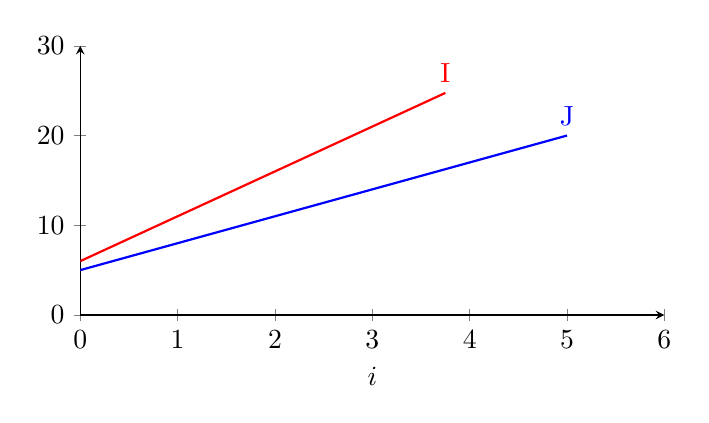
\begin{tikzpicture}
        \begin{axis}[
            axis lines = left,
            xlabel = \(i\),
            ylabel = {},
            domain = 0:5,
            xmin=0,
            xmax=6,
            ymin=0,
            ymax=30,
            restrict y to domain=0:25,
            height=5cm,
            width=9cm,
        ]
        \addplot[thick, color=red]{5*x+6} node[above,pos=1] {I};
        \addplot[thick, color=blue]{3*x+5} node[above,pos=1] {J};
    \end{axis}
    \end{tikzpicture}
\end{minipage}%
\begin{minipage}{.5\textwidth}
    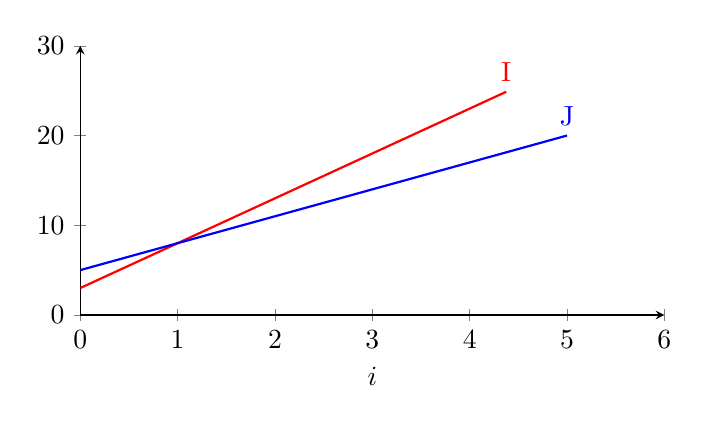
\begin{tikzpicture}
        \begin{axis}[
            axis lines = left,
            xlabel = \(i\),
            ylabel = {},
            domain = 0:5,
            xmin=0,
            xmax=6,
            ymin=0,
            ymax=30,
            restrict y to domain=0:25,
            height=5cm,
            width=9cm,
        ]
        \addplot[thick, color=red]{5*x+3} node[above,pos=1] {I};
        \addplot[thick, color=blue]{3*x+5} node[above,pos=1] {J};
    \end{axis}
    \end{tikzpicture}
\end{minipage}
%[width=5cm]%
    \caption{The image on the left depicts two linear indices $I = 5i+6$ and $J= 3i+5$ as functions of $i$ that do not intersect in the non-negative valuation space of $i$. On the right, we subtract $3$ from $I$, shifting the intersection of $I$ and $J$ into the non-negative valuation space. Thus, $\{i\};\cdot\vDash J \leq I$ but $\{i\};\cdot\nvDash J \leq I-3$. }
    \label{fig:srnecess}
\end{figure}
%
%\includegraphics[width=13cm]{image.png}\\
%Subtracting $3$ from $f$ is enough to shift the intersection of $f$ and $g$ into the non-negative valuation space. Thus, to prove the soundness of an implementation of the type system, it is crucial to have a strong subject reduction property.\\

As we are not interested in actually using a subject reduction property in practice, we can introduce two versions of the implementation: One with type annotations on restrictions, and one without. That is, one without a subject reduction property, and one with a subject reduction property. Intuitively, if $\varphi;\Phi;\Gamma\vdash P \triangleleft \kappa$ by the type system with annotations, then also $\varphi;\Phi;\Gamma\vdash P \triangleleft \kappa$ by the type system without annotations, and so it suffices to prove soundness for the type system without type annotations, to show that any bound on $\kappa$ is an upper bound on the span. Thus, in the remainder of this section, we assume that restrictions do not have type annotations.

%As our restrictions have type annotations, and as annotations advance the time of a context, the structural congruence definition must be augmented to prove a subject congruence result. Consider for instance the process $n : \newvar{a : \texttt{ch}^\sigma_I(\widetilde{T})}{\inputch{a}{\widetilde{v}}{}{P}}$ with some typing $\varphi;\Phi;\Gamma\vdash n : \newvar{a : \texttt{ch}^\sigma_I(\widetilde{T})}{\inputch{a}{\widetilde{v}}{}{P}} \triangleleft \kappa + I + n$ with $\varphi;\Phi;\downarrow_n\!\!\Gamma,a:\texttt{ch}^\sigma_I(\widetilde{T})\vdash \inputch{a}{\widetilde{v}}{}{P} \triangleleft \kappa + I$. Then $\newvar{a : \texttt{ch}^\sigma_I(\widetilde{T})}{n : \inputch{a}{\widetilde{v}}{}{P}}$ is not typable whenever $\varphi;\Phi\nvDash n\leq I$. However, we can quickly verify that $\varphi;\Phi;\Gamma\vdash \newvar{a : \texttt{ch}^\sigma_{I+n}(\widetilde{T})}{n : \inputch{a}{\widetilde{v}}{}{P}} \triangleleft \kappa + I + n$. Thus, if we \textit{delay} or advance the time of a type annotation upon a time annotation in and out (respectively) of the scope of the corresponding restriction, then the subject congruence property holds. Therefore, we formalize \textit{delaying} of types in Definition \ref{def:delayy}. 
%
%if intuitively $\varphi;\Phi;\Gamma,a:\text{delay}(\varphi,\Phi,\Gamma,\iota)\vdash \iota : P \triangleleft K$ where $I$ is the advancement of time imposed by $\iota$.
%

%
% We augment the structural congruence rule $\runa{SC-ares}$ correspondingly
% \begin{align*}
%     \runa{SC-ares}\; n : \newvar{a:T}{P} \equiv \newvar{a:T^{+n}}{n : P}
% \end{align*}
% %
% Moreover, we assume the subsequent rules for restrictions are extended with type annotations. Note that the changes to $\runa{SC-ares}$ do not affect the existence of a canonical form, as we can always apply $\runa{SC-ares}$ from left to right (As we do in the proof of Lemma \ref{lemma:anncannform}), as $T^{+n}$ is defined for any $n$ whenever $T$ is defined.
% %
% % \begin{align*}
%     \text{delay}(\varphi,\Phi,\Gamma,\epsilon, T) =&\; T \\
%     %
%     \text{delay}(\varphi,\Phi,\Gamma,(1,\widetilde{\iota}), T) =&\; \text{delay}(\varphi,\Phi,\susume{\Gamma}{\varphi}{\Phi}{1},\widetilde{\iota},T+1)\\
%     %
%     \text{delay}(\varphi,\Phi,(\Gamma,a:\texttt{ch}^\sigma_I(\widetilde{T})),(a(\widetilde{v})^n_\epsilon,\widetilde{\iota}), T) =&\; \text{delay}(\varphi,\Phi,(\susume{\Gamma}{\varphi}{\Phi}{I},a:\texttt{ch}^\sigma_0(\widetilde{T})),\widetilde{\iota},T+I)\\
%     %
%     \text{delay}(\varphi,\Phi,(\Gamma,a:\forall_I\widetilde{i}.\texttt{serv}^\sigma_K(\widetilde{T})),(a(\widetilde{v})^n_{\widetilde{e}},\widetilde{\iota}), T) =&\; \text{delay}(\varphi,\Phi,(\susume{\Gamma}{\varphi}{\Phi}{I},a:\forall_I\widetilde{i}.\texttt{serv}^\sigma_K(\widetilde{T})),\widetilde{\iota},T+I)
% \end{align*}
%\end{defi}
%

% We now define the local complexity of an augmented process based on its prefix of annotations in Definition \ref{def:lcbg}. Specifically, a tick has a cost of one in time complexity, and so the $1$-annotation adds one to the local complexity. Channel annotations $a(\widetilde{v})^n_{\widetilde{e}}$ are more complex, as we treat the constant $n$ similarly to the time $I$ of a channel type $\texttt{ch}^\sigma_I(\widetilde{T})$, in that it is relative. For instance, in a typing $\varphi;\Phi;\cdot,a:\texttt{ch}^{\{\texttt{in}\}}_I(\widetilde{T}),b:\texttt{ch}^{\{\texttt{out}\}}_J(\widetilde{S}) \vdash \inputch{a}{\widetilde{v}}{}{\tick\asyncoutputch{b}{\widetilde{e}}{}} \triangleleft J$, we type $\asyncoutputch{b}{\widetilde{e}}{}$ under the context $\cdot,a:\texttt{ch}^{\{\texttt{in}\}}_0(\widetilde{T}),b:\texttt{ch}^{\{\texttt{out}\}}_{J-I-1}(\widetilde{S})$, and so the bound on the complexity is $I+1+(J-I-1)=J$ as $\varphi;\Phi\vDash I+1 \leq J$ by definition of advancement of time. In the same sense, each constant added to the local complexity is subtracted from all succeeding channel annotations, and so local complexity has the following properties. If $\mathcal{C}_\ell(\widetilde{\iota} : G) \geq n$ then $\mathcal{C}_\ell(\widetilde{\iota} : a(\widetilde{v})^n_{\widetilde{e}} : G)=\mathcal{C}_\ell(\widetilde{\iota} : G)$ and if $\mathcal{C}_\ell(\widetilde{\iota} : G) \leq n$ then $\mathcal{C}_\ell(\widetilde{\iota} : a(\widetilde{v})^n_{\widetilde{e}} : G)=n$. Thus, if we are careful with how channel annotations are introduced, then this definition of local complexity is equivalent to the one in Definition \ref{def:bglcsim}.
% %
% \begin{defi}[Local complexity]\label{def:lcbg}
% We define the local complexity $\mathcal{C}_\ell(P)$ of an augmented process $P$ inductively
% %\begin{align*}
% \begin{alignat*}{3}
%     \mathcal{C}_\ell(1 : P) =&&\; 1 + \mathcal{C}_\ell(P^{-1})\qquad\qquad\qquad\kern1em (1 : P)^{-n} =&&\; 1 : P^{-n}\kern3em\;\;\\
%     \mathcal{C}_\ell(a(\widetilde{v})^n_{\widetilde{e}} : P) =&&\; n + \mathcal{C}_\ell(P^{-n})\qquad\qquad\kern0.5em (a(\widetilde{v})^m_{\widetilde{e}} : P)^{-n} =&&\; a(\widetilde{v})^{m-n}_{\widetilde{e}} : P^{-n}\;\\
%     \mathcal{C}_\ell(P \mid Q) =&&\; \text{max}(\mathcal{C}_\ell(P),\mathcal{C}_\ell(Q))\qquad\qquad (P\mid Q)^{-n} =&&\; P^{-n} \mid Q^{-n}\kern2em\\
%     \mathcal{C}_\ell(\newvar{a : T}{P}) =&&\; \mathcal{C}_\ell(P)\qquad\qquad\qquad\kern1em (\newvar{a:T}{_{\widetilde{\iota}}\; P})^{-n} =&&\; \newvar{a:T}{_{\widetilde{\iota}}\; P^{-n}}\;\;\;\\
%     \mathcal{C}_\ell(G) =&&\; 0 \qquad\qquad\qquad\kern8em G^{-n} =&&\; G\kern6em
% \end{alignat*}
% \end{defi}
% As expressions may now be annotated with variables, we must be careful when transmitting an expression over a channel. That is, the annotated variable may be bound in a channel annotation, and so it may be free in the process that receives the expression. To account for this, we introduce the notation $\circledcirc e$ in Definition \ref{def:annotrembg} that represents the expression $e$ with all annotations removed. As annotations solely guide subtyping, we can deduce that if we can assign some type $T$ to $e$, then we can assign a super type of $T$ to $\circledcirc e$. We formalize this result in Section \ref{sec:intermelemmabg}.
% \begin{defi}\label{def:annotrembg}
% We define the notation $\circledcirc e$ to denote $e$ without annotations, defined inductively by the rules
% \begin{align*}
%     \circledcirc e_\theta = \circledcirc e\kern2em  \circledcirc\! 0 = 0\kern2em\circledcirc \succc{e} = \s(\circledcirc e)\kern2em \circledcirc\! v = v
%     %\circledcirc 0 =&\; 0\\
%     %\circledcirc v =&\; v
% \end{align*}
% \end{defi}
% %
% In Definition \ref{tab:parallelredurules}, we now introduce the parallel reduction relation $\Longrightarrow$ for augmented processes. Tick prefixes reduce to $1$-annotations by rule $\runa{PR-tick}$. For pattern matches on a natural of the form $\succc{e}_{\widetilde{\theta}}$, we substitute $e_{\succc{e}_{\widetilde{\theta}}}$ for the variable bound in the successor pattern. Here, the annotation provides information about the typing of $\succc{e}$ prior to reduction, such that we can type $e$ accordingly subject to subtyping. The most notable rules are $\runa{PR-rep}$ and $\runa{PR-comm}$ that synchronize annotated inputs and outputs on servers and normal channels, respectively. We annotate the continuation of the input with the annotation prefix of the input extended with a channel annotation marked with the maximum of the local complexities of the prefixes of the input and output. Thus, the local complexity of the new annotation prefix is equal to the local complexity of the parallel composition prior to reduction. We substitute $(\circledcirc \widetilde{e})_{\widetilde{v}}$ for the variables bound in the input $\widetilde{v}$, where $\widetilde{e}$ are the expressions of the output and $(\circledcirc \widetilde{e})_{\widetilde{v}}=(\circledcirc e_1)_{v_1},\dots,(\circledcirc e_n)_{v_n}$. Here, we use the notation $\circledcirc e$ to remove annotations that potentially contain variables bound in the annotation prefix of the output, i.e. they are free in the input process. We annotate the expressions with the variables they replace, to provide information for subtyping when typing the process after reduction.\\

% %
% \begin{table*}[ht]
%     \centering
%     \begin{framed}\vspace{-1em}\begin{align*}
%         &\kern0em\runa{PR-rep}\;\;\condinfrule{}{\parcomp{\widetilde{\iota}_1 : \;\bang{\inputch{a}{\widetilde{v}}{}{P}}}{\widetilde{\iota}_2 : \asyncoutputch{a}{\widetilde{e}}{}} \Longrightarrow \parcomp{\widetilde{\iota}_1 : \;\bang{\inputch{a}{\widetilde{v}}{}{P}}}{\widetilde{\iota}_2 : a(\widetilde{v})^n_{\widetilde{e}} :\subst{P}{\widetilde{v}\mapsto (\circledcirc\widetilde{e})_{\widetilde{v}}}}}{\!\!\!\!\!\!\!\!\!\!\text{where}\; n = \text{max}(\mathcal{C}_\ell(\widetilde{\iota}_1 : \nil),\mathcal{C}_\ell(\widetilde{\iota}_2 : \nil))}\\
%         %
%         &\kern0em\runa{PR-comm}\;\;\condinfrule{}{\widetilde{\iota}_1 :\inputch{a}{\widetilde{v}}{}{P}
%         \mid 
%         \widetilde{\iota}_2 : \asyncoutputch{a}{\widetilde{e}}{} \Longrightarrow \widetilde{\iota}_1 : a(\widetilde{v})^n_{\epsilon} : \subst{P}{\widetilde{v}\mapsto (\circledcirc\widetilde{e})_{\widetilde{v}}}}{\text{where}\; n = \text{max}(\mathcal{C}_\ell(\widetilde{\iota}_1 : \nil),\mathcal{C}_\ell(\widetilde{\iota}_2 : \nil))}\\[-1em]
%         %
%         &\kern0em\runa{PR-zero}\;\;\infrule{}{\match{0_{\widetilde{\theta}}}{P}{x}{Q} \Longrightarrow P}
%         %
%         \kern6em\runa{PR-par}\;\;\infrule{P \Longrightarrow Q}{\parcomp{P}{R} \Longrightarrow \parcomp{Q}{R}}
%         \\[-1em]
%         %
%         &\kern0em\runa{PR-succ}\;\;\infrule{}{\match{\succc{e}_{\widetilde{\theta}}}{P}{x}{Q} \Longrightarrow Q[x \mapsto e_{\succc{e}_{\widetilde{\theta}}}]}  \\[-1em]
%         %
%         %\kern0em\runa{PR-empty}\;\;\infrule{}{\texttt{match}\; []_{\widetilde{\theta}}\; \{ [] \mapsto P; x :: y \mapsto Q \} \Longrightarrow P} \\[-1em]
%         %
%         &\runa{PR-annot}\infrule{P \Longrightarrow Q}{\iota : P \Longrightarrow \iota : Q}\kern6em \runa{PR-res}\;\;\infrule{P \Longrightarrow Q}{\newvar{a : T}{_{\widetilde{\iota}}\; P} \Longrightarrow \newvar{a : T}{_{\widetilde{\iota}}\;Q}}
%         \\[-1em]
%         %
%         %\kern7em\runa{PR-cons}\;\;\infrule{}{\texttt{match}\; (e :: e')_{\widetilde{\theta}}\; \{ [] \mapsto P; x :: y \mapsto Q \} \Longrightarrow Q[x \mapsto e,y \mapsto e_{\widetilde{\theta},-1}']}\\[-1em]
%         %
%         %\kern3em\runa{R-par}\;\;\infrule{P \longrightarrow Q}{\parcomp{P}{R} \longrightarrow \parcomp{Q}{R}} \kern-0em \runa{R-res}\;\;\infrule{P \longrightarrow Q}{\newvar{a}{P} \longrightarrow \newvar{a}{Q}}\\
%         %
%         &\kern4em\runa{PR-struct}\;\;\infrule{P \equiv P'\quad P' \Longrightarrow Q'\quad Q' \equiv Q}{P \Longrightarrow Q} \kern1em \runa{PR-tick}\;\;\infrule{}{\tick P \Longrightarrow 1 : P}\kern5.5em\text{ }
%     \end{align*}\end{framed}
%     \smallskip
%     \caption{The parallel reduction rules defining $\Longrightarrow$.}
%     \label{tab:parallelredurules}
% \end{table*}
% %
% %
% Finally, in Definition \ref{def:pcbga} we define the parallel complexity of an augmented process $P$ to be equal to the maximum local complexity amongst process $P$ and processes that $P$ can reduce to.
% %
% \begin{defi}[Parallel complexity]\label{def:pcbga}
% Let $P$ be an augmented process, then we define the parallel complexity of $P$ as
% \begin{align*}
%     \mathcal{C}_\mathcal{P}(P) = \text{max}\{ \mathcal{C}_\ell(Q) \mid P \Longrightarrow^* Q \}
% \end{align*}
% where $\Longrightarrow^*$ is the transitive and reflexive closure of $\Longrightarrow$.
% \end{defi}

% \subsection{Annotated type rules}\label{sec:anntyperulebg}

% % $\varphi;\Phi;\Gamma;\Delta\vdash^m_J P \triangleleft K$ $\varphi;\Phi;\Gamma;\Delta\vdash e : T$.

% \begin{table*}[ht]
%     \begin{framed}\vspace{-1em}\begin{align*}
%         &\kern-6em
%         \runa{S-zero}\;\infrule{}{\varphi;\Phi;\Gamma;\Delta\vdash\withtype{0}{\typenat[0,0]}}\kern0em
%         \runa{S-succ}\;\infrule{\varphi;\Phi;\Gamma;\Delta \vdash \withtype{e}{\typenat[I, J]}}{\varphi;\Phi;\Gamma;\Delta \vdash \withtype{\succc{e}}{\typenat[I + 1, J + 1]}}\\[-1em]
%         %
%         %&\kern-8em\runa{S-empty}\;\infrule{}{\varphi;\Phi;\Gamma\vdash_\Delta\withtype{[]}{\texttt{List}[0,0](\mathcal{B})}}\kern0em
%         %\runa{S-cons}\;\infrule{\varphi;\Phi;\Gamma\vdash_{\Delta} e : \mathcal{B} \quad\varphi;\Phi;\Gamma \vdash_\Delta \withtype{e'}{\texttt{List}[I, J](\mathcal{B}')}}{\varphi;\Phi;\Gamma \vdash_\Delta \withtype{e :: e'}{\texttt{List}[I + 1, J + 1](\mathcal{B} \uplus_{\varphi;\Phi} \mathcal{B}')}}\\[-1em]
%         %
%         &%\runa{S-cons-2}\;\infrule{\varphi;\Phi;\Gamma\vdash e : \mathcal{B} \quad\varphi;\Phi;\Gamma \vdash \withtype{e'}{\texttt{List}[0, 0](\mathcal{B}')}}{\varphi;\Phi;\Gamma \vdash \withtype{e :: e'}{\texttt{List}[1, 1](\mathcal{B})}}\quad\quad\quad\quad\quad\quad\quad
%         %
%         \kern-6em\runa{S-var}\;\infrule{}{\varphi;\Phi;\Gamma, \withtype{v}{T};\Delta \vdash \withtype{v}{T}}
%         \runa{S-avar}\;\infrule{\varphi;\Phi;\Gamma;\Delta,v:T\vdash e : S\quad \varphi;\Phi\vdash S \sqsubseteq T}{\varphi;\Phi;\Gamma;\Delta,v:T\vdash e_v : T}\\
%         %
%         &\kern-9em\runa{S-strength}\; \infrule{\varphi;\Phi;\Gamma;\Delta\vdash e : \texttt{Nat}[I',J']\quad \varphi;\Phi;\Gamma;\Delta\vdash e' : \texttt{Nat}[I,J]\quad \varphi;\Phi\vdash \texttt{Nat}[I',J']\sqsubseteq \texttt{Nat}[I-1,J-1]}{\varphi;\Phi;\Gamma;\Delta\vdash e_{e'} : \texttt{Nat}[I-1,J-1]}%\\
%         %
%         %&\kern-10em\runa{S-strength-2}\; \infrule{\varphi;\Phi;\Gamma\vdash_\emptyset \circledcirc e : \texttt{List}[I',J'](\mathcal{B}')\quad \varphi;\Phi;\Gamma\vdash_\Delta e : \texttt{List}[I,J](\mathcal{B})\quad \varphi;\Phi\vdash \texttt{List}[I',J'](\mathcal{B}')\sqsubseteq \texttt{List}[I-1,J-1](\mathcal{B})}{\varphi;\Phi;\Gamma\vdash_\Delta e_{-1} : \texttt{List}[I-1,J-1](\mathcal{B})}
%     \end{align*}\vspace{-1em}\end{framed}
%     \smallskip
%     \caption{Extended type rules for expressions.}
%     \label{tab:sizedannottypedexpressiontypes}
% \end{table*}

% \begin{table*}[!ht]
%     \begin{framed}\vspace{-1em}\begin{align*}
%         &\kern15em\\[-2em] % Stretch frame
%         &\kern0em\runa{SA-nil}\infrule{}{\varphi;\Phi;\Gamma;\Delta \vdash_{J} \withcomplex{\nil}{\{0\}}}
%         %
%         \kern3em\runa{SA-tick}\;\infrule{\varphi;\Phi;\susumesim{\Gamma}{1};\downarrow_1\!\!\Delta\vdash_{J+1} P \triangleleft \kappa}{\varphi;\Phi;\Gamma;\Delta\vdash_{J} \tick P \triangleleft \kappa + 1}\\[-1em]
%         %
%         &\kern-0em\runa{SA-match}\;\infrule{
%         \begin{matrix}
%             \varphi;\Phi;\Gamma;\Delta \vdash \withtype{e}{\natinterval{I}{J}}\quad \varphi;\Phi, I \leq 0;\Gamma;\Delta \vdash_{L} \withcomplex{P}{\kappa} \\
%             \varphi;\Phi, J \geq 1;\Gamma, \withtype{x}{\natinterval{I-1}{J-1}};\Delta \vdash_{L} \withcomplex{Q}{\kappa'}
%         \end{matrix}}{\varphi;\Phi;\Gamma;\Delta \vdash_{L} \withcomplex{\match{e}{P}{x}{Q}}{\text{basis}(\varphi,\Phi,\kappa\cup\kappa')}}\\[-1em]
%         %
%         %&\kern-0em\runa{S-nmatch-2}\;\infrule{
%         %\begin{matrix}
%         %    \varphi;\Phi;\Gamma \vdash \withtype{e}{\natinterval{I}{J}} \quad \varphi;\Phi\vDash K \leq K' \\
%         %    \varphi;\Phi, I \leq 0;\Gamma \vdash \withcomplex{P}{K} \quad \varphi;\Phi, J \geq 1;\Gamma, \withtype{x}{\natinterval{I-1}{J-1}} \vdash \withcomplex{Q}{K'}
%         %\end{matrix}}{\varphi;\Phi;\Gamma \vdash \withcomplex{\match{e}{P}{x}{Q}}{K'}}\\[-1em]
%         %
%         %&\kern-0em\runa{SA-lmatch}\;\condinfrule{
%         %\begin{matrix}
%         %    \varphi;\Phi;\Gamma \vdash \withtype{e}{\texttt{List}[I,J](\mathcal{B})} \quad \varphi;\Phi, I \leq 0;\Gamma \vdash^m_L \withcomplex{P}{K} \\
%         %    \varphi;\Phi, J \geq 1;\Gamma, \withtype{x}{\mathcal{B}},y : \texttt{List}[I-1,J-1](\mathcal{B}) \vdash^m_L \withcomplex{Q}{K'}
%         %\end{matrix}}{\varphi;\Phi;\Gamma \vdash^m_L \withcomplex{\texttt{match}\;e\;\{ [] \mapsto P;\; x :: y \mapsto Q \}}{L}}{\text{where}\quad L = \left\{
% %\begin{matrix}
% %    K & \text{if}\; \varphi;\Phi\vDash K' \leq K   \\
% %    K' & \text{if}\; \varphi;\Phi\vDash K \leq K'  %\\
%     %K+K' & \text{otherwise}
% %\end{matrix}
% %\right.}\\[-1em]
%         %
%         %&\kern-0em\runa{S-lmatch-2}\;\infrule{
%         %\begin{matrix}
%         %    \varphi;\Phi;\Gamma \vdash \withtype{e}{\texttt{List}[I,J](\mathcal{B})} \quad \varphi;\Phi\vDash K \leq K' \\
%         %    \varphi;\Phi, I \leq 0;\Gamma \vdash \withcomplex{P}{K} \quad \varphi;\Phi, J \geq 1;\Gamma, \withtype{x}{\mathcal{B}},y : \texttt{List}[I-1,J-1](\mathcal{B}) \vdash \withcomplex{Q}{K'}
%       % \end{matrix}}{\varphi;\Phi;\Gamma \vdash \withcomplex{\texttt{match}\;e\;\{ [] \mapsto P;\; x :: y \mapsto Q \}}{K'}}\\[-1em]
%         %
%         %&\kern4em\runa{SA-par}\;\condinfrule{\varphi;\Phi;\Gamma;\Delta\vdash^m_{J} P \triangleleft K\quad \varphi;\Phi;\Gamma;\Delta\vdash^m_{J} Q \triangleleft K'}{\varphi;\Phi;\Gamma;\Delta\vdash^m_{J} \parcomp{P}{Q} \triangleleft L}{\text{where}\quad L = \left\{
% %\begin{matrix}
% %    K & \text{if}\; \varphi;\Phi\vDash K' \leq K   \\
% %    K' & \text{if}\; \varphi;\Phi\vDash K \leq K'  %\\
%     %K+K' & \text{otherwise}
% %\end{matrix}
% %\right.}\\[-1em]
% %
% &\kern-0em\runa{SA-par}\;\infrule{\varphi;\Phi;\Gamma;\Delta\vdash_J P \triangleleft \kappa\quad \varphi;\Phi;\Gamma;\Delta\vdash_J Q \triangleleft \kappa'}{\varphi;\Phi;\Gamma;\Delta\vdash_J P \mid Q \triangleleft \text{basis}(\varphi,\Phi,\kappa\cup\kappa')}
% %
% \kern8em\runa{SA-nu}\;\infrule{\varphi;\Phi;\Gamma,\withtype{a}{\text{delay}(\varphi,\Phi,\Gamma,\widetilde{\iota},T)};\Delta \vdash_{J} \withcomplex{P}{\kappa}}{\varphi;\Phi;\Gamma;\Delta \vdash_{J} \newvar{a: T}{_{\widetilde{\iota}}\; P}\triangleleft \kappa} \\[-1em]
% %
% %&\runa{SA-par-fail}\;\condinfrule{\varphi;\Phi;\Gamma;\Delta\vdash^m_J P \triangleleft K;\kappa\quad \varphi;\Phi;\Gamma;\Delta\vdash^m_J Q \triangleleft K';\kappa'\quad \forall L\in\kappa''.\exists L'\in\kappa''.\varphi;\Phi\nvDash L' \leq L}{\varphi;\Phi;\Gamma;\Delta\vdash^m_J P \mid Q \triangleleft 0; \kappa''}{\kappa'' = \kappa \cup \kappa' \cup \{K,K'\}}    \\[-1em]
% %
%         %
%         %&\kern4em\runa{S-par-2}\;\infrule{\varphi;\Phi;\Gamma\vdash P \triangleleft K\quad \varphi;\Phi;\Gamma\vdash Q \triangleleft K'\quad \varphi;\Phi\vDash K \leq K'}{\varphi;\Phi;\Gamma\vdash \parcomp{P}{Q} \triangleleft K'}\\[-1em]
%         %
%         &\kern-0em\runa{SA-iserv}\;\infrule{\texttt{in}\in\sigma\quad \varphi,\widetilde{i};\Phi;\text{ready}(\varphi,\Phi,\susumesim{\Gamma}{I}),a:\forall_0\widetilde{i}.\texttt{serv}^{\sigma\cap\{\texttt{out}\}}_K(\widetilde{T}),\widetilde{v} : \widetilde{T};\text{ready}(\varphi,\Phi,\susumesim{\Delta}{I})\vdash_{J+I} P \triangleleft \kappa\quad\varphi,\widetilde{i};\Phi\vDash \kappa \leq K}{\varphi;\Phi;\Gamma,a:\forall_I\widetilde{i}.\texttt{serv}^\sigma_K(\widetilde{T});\Delta\vdash_{J}\; \bang\inputch{a}{\widetilde{v}}{}{P}\triangleleft \{I\}}\\[-1em]
%         %
%         &\kern-0em\runa{SA-ich}\;\infrule{\texttt{in}\in\sigma\quad \varphi;\Phi;\susumesim{\Gamma}{I},a:\texttt{ch}_0^\sigma(\widetilde{T}),\widetilde{v} : \widetilde{T};\Delta\vdash_{J+I} P \triangleleft \kappa}{\varphi;\Phi;\Gamma,a:\texttt{ch}_I^\sigma(\widetilde{T});\Delta\vdash_{J} \inputch{a}{\widetilde{v}}{}{P}\triangleleft \kappa + I}\\[-1em]
%         %
%         &\kern-0em\runa{SA-och}\;\infrule{\texttt{out}\in \sigma\quad \varphi;\Phi;\susumesim{\Gamma}{I};\Delta\vdash \widetilde{e} : \widetilde{T}\quad \varphi;\Phi\vdash\widetilde{T}\sqsubseteq\widetilde{S}}{\varphi;\Phi;\Gamma,a:\texttt{ch}^{\sigma}_I(\widetilde{S});\Delta\vdash_{J} \asyncoutputch{a}{\widetilde{e}}{} \triangleleft \{I\}}
%         %
%         \kern12em\runa{SA-atick}\;\infrule{\varphi;\Phi;\downarrow_1\!\!\Gamma;\downarrow_1\!\!\Delta\vdash_{J+1} P \triangleleft \kappa}{\varphi;\Phi;\Gamma;\Delta\vdash_{J} 1 : P \triangleleft \kappa + 1}
%         \\[-1em]
%         %
%         &\kern0em\runa{SA-oserv}\;\infrule{\texttt{out} \in \sigma\quad \varphi;\Phi;\susumesim{\Gamma}{I};\cdot\vdash \circledcirc\widetilde{e} : \widetilde{T}\quad \text{instantiate}(\widetilde{i},\widetilde{T})=\{\widetilde{J}/\widetilde{i}\}\quad  \varphi;\Phi\vdash\widetilde{T}\sqsubseteq\widetilde{S}\{\widetilde{J}/\widetilde{i}\}}{\varphi;\Phi;\Gamma,a:\forall_I\widetilde{i}.\texttt{serv}_K^\sigma(\widetilde{S});\Delta\vdash_{L} \asyncoutputch{a}{\widetilde{e}}{} \triangleleft \{K\!\substi{\widetilde{J}}{\widetilde{i}} + I\}}\\[-1em]
%         %
%         &\kern0em\runa{SA-aich}\;\infrule{\varphi;\Phi\vDash n \leq I + J\quad \varphi;\Phi;\downarrow_I\!\!\Gamma,a:\texttt{ch}^\sigma_0(\widetilde{T});\downarrow_I\!\!\Delta,\widetilde{v}:\widetilde{T}\vdash_{J+I} P \triangleleft \kappa}{\varphi;\Phi;\Gamma,a : \texttt{ch}^\sigma_I(\widetilde{T});\Delta\vdash_{J} a(\widetilde{v})^n_\epsilon : P \triangleleft \kappa + I}\\
%         %
%         &\kern0em\runa{SA-aiserv}\;\infrule{
%         \begin{matrix}
%             \varphi;\Phi\vDash n \leq I + J\quad \varphi;\Phi;\downarrow_I\!\!\Gamma;\cdot\vdash \circledcirc\widetilde{e} : \widetilde{S} \quad \text{instantiate}(\widetilde{i},\widetilde{S})=\{\widetilde{L}/\widetilde{i}\}\\ 
%             %\varphi;\Phi\vdash \widetilde{S} \sqsubseteq \widetilde{T}\{\widetilde{L}/\widetilde{i}\}\quad
%             %
%             \varphi;\Phi;\downarrow_I\!\!\Gamma,a:\forall_0\widetilde{i}.\texttt{serv}^{\sigma\cap\{\texttt{out}\}}_K(\widetilde{T});\downarrow_I\!\!\Delta,\widetilde{v}:\widetilde{T}\{\widetilde{L}/\widetilde{i}\}\vdash_{J+I} P \triangleleft \kappa %\quad\varphi,\widetilde{i};\Phi\vDash \kappa \leq K\{\widetilde{L}/\widetilde{i}\}
%         \end{matrix}
%         }{\varphi;\Phi;\Gamma, a : \forall_I\widetilde{i}.\texttt{serv}^\sigma_K(\widetilde{T});\Delta\vdash_{J} a(\widetilde{v})^n_{\widetilde{e}} : P \triangleleft \kappa + I}
%     \end{align*}\vspace{-1em}\end{framed}
%     \smallskip
%     \caption{Sized typing rules for parallel complexity of annotated processes.}
%     \label{tab:sizedannotatedprocesstypingrules}
% \end{table*}

\subsection{Intermediary lemmas}\label{sec:intermelemmabg}
We are now ready to present the soundness results. We first prove some intermediary lemmas that we use for the main results. We first prove some useful properties with respect to delaying in Lemma \ref{lemma:delayingg}. We use the first point in the clause of $\runa{SC-ares}$ in the proof of subject congruence. We use the second and third points for the proof of subject reduction, namely for synchronizations on channels, where we preserve the maximal local complexity amongst an input and output, and so we may need to \textit{delay} the type context.
%
\begin{lemma}[Delaying]\label{lemma:delayingg}\text{ }
\begin{enumerate}
    \item $\susume{\uparrow^I\!\!T}{\varphi}{\Phi}{I}=T$.
    \item If $\varphi;\Phi;\Gamma\vdash e : T$ then $\varphi;\Phi;\uparrow^I\!\!\Gamma\vdash e : \uparrow^I\!\!T$.
    \item If $\varphi;\Phi;\Gamma\vdash P \triangleleft \kappa$ then $\varphi;\Phi;\uparrow^I\!\!\Gamma\vdash P \triangleleft \kappa + I$.
\end{enumerate}
\begin{proof} Point $1$ is straightforward. Point $2$ and $3$ are proved by induction on the type rules of expressions and processes, respectively.
\end{proof}
\end{lemma}
%
We next prove that advancement of time is additive. This result is integral to subject congruence, namely for $\runa{SC-sum}$ that allows us to sum two annotations, and correspondingly split one annotation into two. 
%
\begin{lemma}[Additive advancement of time]\label{lemma:addsusume}
Let $\Phi$ be a set of constraints with unknowns in $\varphi$ and let $T$ be a type then $\susume{\susume{T}{\varphi}{\Phi}{J}}{\varphi}{\Phi}{I} =\; \susume{T}{\varphi}{\Phi}{I+J}$.
 \begin{proof} On the structure of $T$. The proof is shown in Appendix \ref{app:sizedtypesoundness}.
%     \begin{description}
%     \item[$(\susume{\susume{\mathcal{B}}{\varphi}{\Phi}{J}}{\varphi}{\Phi}{I})$] obtained directly from  $\susume{\mathcal{B}}{\varphi}{\Phi}{J} = \mathcal{B}$ and $\susume{\mathcal{B}}{\varphi}{\Phi}{I} = \mathcal{B}$.
%     %
%     \item[$(\susume{\susume{\texttt{ch}^\sigma_L(\widetilde{T})}{\varphi}{\Phi}{J}}{\varphi}{\Phi}{I})$] We either have that
%     \begin{enumerate}
%         \item $\varphi;\Phi\vDash J \leq L$ and so we have that $\susume{\texttt{ch}^\sigma_L(\widetilde{T})}{\varphi}{\Phi}{J}=\texttt{ch}^\sigma_{L-J}(\widetilde{T})$. Then if $\varphi;\Phi\vDash I \leq L-J$ we also have $\varphi;\Phi\vDash I+J \leq L$ as $\varphi;\Phi\vDash J \leq L$, and so we obtain $\susume{\susume{\texttt{ch}^\sigma_L(\widetilde{T})}{\varphi}{\Phi}{J}}{\varphi}{\Phi}{I}=\susume{\texttt{ch}^\sigma_L(\widetilde{T})}{\varphi}{\Phi}{I+J}=\texttt{ch}^\sigma_{L-(I+J)}(\widetilde{T})$. Otherwise, we have that $\varphi;\Phi\nvDash I \leq L-J$, implying that $\varphi;\Phi\nvDash I+J \leq L$ as $\varphi;\Phi\vDash J \leq L$, and so we obtain $\susume{\susume{\texttt{ch}^\sigma_L(\widetilde{T})}{\varphi}{\Phi}{J}}{\varphi}{\Phi}{I}=\susume{\texttt{ch}^\sigma_L(\widetilde{T})}{\varphi}{\Phi}{I+J}=\texttt{ch}^\emptyset_{L-(I+J)}(\widetilde{T})$.
%         %
%         \item $\varphi;\Phi\nvDash J \leq L$ and so we have that $\susume{\texttt{ch}^\sigma_L(\widetilde{T})}{\varphi}{\Phi}{J}=\texttt{ch}^\emptyset_{L-J}(\widetilde{T})$ and $\susume{\texttt{ch}^\emptyset_{L-J}(\widetilde{T})}{\varphi}{\Phi}{I}=\texttt{ch}^\emptyset_{(L-J)-I}(\widetilde{T})$. It follows from the fact that $I$ is non-negative that also $\varphi;\Phi\nvDash I+J \leq L$ and so we obtain $\susume{\susume{\texttt{ch}^\sigma_L(\widetilde{T})}{\varphi}{\Phi}{J}}{\varphi}{\Phi}{I}=\texttt{ch}^\emptyset_{L-(J+I)}(\widetilde{T})=\texttt{ch}^\emptyset_{(L-J)-I}(\widetilde{T})$.
%     \end{enumerate}
%     %
%     \item[$(\susume{\susume{\forall_L\widetilde{i}.\texttt{serv}^\sigma_K(\widetilde{T})}{\varphi}{\Phi}{J}}{\varphi}{\Phi}{I})$] We either have that
%     \begin{enumerate}
%         \item $\varphi;\Phi\vDash J \leq L$ and so we have that $\susume{\forall_L\widetilde{i}.\texttt{serv}^\sigma_K(\widetilde{T})}{\varphi}{\Phi}{J}=\forall_{L-J}\widetilde{i}.\texttt{serv}^\sigma_K(\widetilde{T})$. Then if $\varphi;\Phi\vDash I \leq L-J$ we also have $\varphi;\Phi\vDash I+J \leq L$ as $\varphi;\Phi\vDash J \leq L$, and so we obtain $\susume{\susume{\forall_L\widetilde{i}.\texttt{serv}^\sigma_K(\widetilde{T})}{\varphi}{\Phi}{J}}{\varphi}{\Phi}{I}=\susume{\forall_L\widetilde{i}.\texttt{serv}^\sigma_K(\widetilde{T})}{\varphi}{\Phi}{I+J}=\forall_{L-(I+J)}\widetilde{i}.\texttt{serv}^\sigma_K(\widetilde{T})$. Otherwise, we have that $\varphi;\Phi\nvDash I \leq L-J$, implying that $\varphi;\Phi\nvDash I+J \leq L$ as $\varphi;\Phi\vDash J \leq L$, and so we obtain $\susume{\susume{\forall_L\widetilde{i}.\texttt{serv}^\sigma_K(\widetilde{T})}{\varphi}{\Phi}{J}}{\varphi}{\Phi}{I}=\susume{\forall_L\widetilde{i}.\texttt{serv}^\sigma_K(\widetilde{T})}{\varphi}{\Phi}{I+J}=\forall_{L-(I+J)}\widetilde{i}.\texttt{serv}^{\sigma\cap\{\texttt{out}\}}_K(\widetilde{T})$.
%         %
%         \item $\varphi;\Phi\nvDash J \leq L$ and so we have that $\susume{\forall_L\widetilde{i}.\texttt{serv}^\sigma_K(\widetilde{T})}{\varphi}{\Phi}{J}=\forall_{L-J}\widetilde{i}.\texttt{serv}^{\sigma\cap\{\texttt{out}\}}_K(\widetilde{T})$ and $\susume{\forall_{L-J}\widetilde{i}.\texttt{serv}^{\sigma\cap\{\texttt{out}\}}_K(\widetilde{T})}{\varphi}{\Phi}{I}=\forall_{(L-J)-I}\widetilde{i}.\texttt{serv}^{\sigma\cap\{\texttt{out}\}}_K(\widetilde{T})$. It follows from the fact that $I$ is non-negative that also $\varphi;\Phi\nvDash I+J \leq L$ and so we obtain $\susume{\susume{\forall_L\widetilde{i}.\texttt{serv}^\sigma_K(\widetilde{T})}{\varphi}{\Phi}{J}}{\varphi}{\Phi}{I}=\\forall_{L-(I+J)}\widetilde{i}.\texttt{serv}^{\sigma\cap\{\texttt{out}\}}_K(\widetilde{T})=\forall_{(L-J)-I}\widetilde{i}.\texttt{serv}^{\sigma\cap\{\texttt{out}\}}_K(\widetilde{T})$.
%     \end{enumerate}
%     \end{description}
\end{proof}
\end{lemma}
%
We now prove the usual weakening and strengthening lemmas in Lemma \ref{lemma:weakening} and Lemma \ref{lemma:strengthening}, respectively. In this work, we can weaken and strengthen sets of constraints and type contexts. That is, we can safely introduce new constraints or type associations, and discard constraints that are covered by the remaining constraints, as well as type associations for variables that are not free in a corresponding expression or process. As a consequence of type rule $\runa{S-subsumption}$, it is also safe to use subtyping on contexts.
%
\begin{lemma}[Weakening]\label{lemma:weakening}
Let $\Gamma$ and $\Gamma'$ be disjoint contexts. Then
\begin{enumerate}
    \item If $\varphi;\Phi;\Gamma\vdash e : T$ then $\varphi,\varphi';\Phi,\Phi';\Gamma,\Gamma'\vdash e : T$.
    %
    %\item If $\varphi;\Phi;\Gamma;\Delta\vdash^m_{J} P \triangleleft K$ and $n\leq m$ then also $\varphi;\Phi;\Gamma;\Delta\vdash^n_J P \triangleleft K$.
    %
    \item If $\varphi;\Phi;\Gamma\vdash P \triangleleft \kappa$ then $\varphi,\varphi';\Phi,\Phi';\Gamma,\Gamma'\vdash P \triangleleft \kappa$.
    %
    \item If $\varphi;\Phi;\Gamma\vdash e : T$ and $\varphi;\Phi\vdash \Delta \sqsubseteq \Gamma$ then $\varphi;\Phi;\Delta\vdash e : T$.
    %
    \item If $\varphi;\Phi;\Gamma\vdash P \triangleleft \kappa$ and $\varphi;\Phi\vdash \Delta \sqsubseteq \Gamma$ then $\varphi;\Phi;\Delta\vdash P \triangleleft \kappa$.
    %
    % \item If $\varphi;\Phi;\Gamma,a:\texttt{ch}^\sigma_I(\widetilde{T})\vdash P \triangleleft \kappa$ and $\sigma \subseteq \sigma'$ then also $\varphi;\Phi;\Gamma,a:\texttt{ch}^{\sigma'}_I(\widetilde{T})\vdash P \triangleleft \kappa$. 
    % %
    % \item If $\varphi;\Phi;\Gamma,a:\forall_I\widetilde{i}.\texttt{serv}_L^\sigma(\widetilde{T})\vdash P \triangleleft \kappa$ and $\sigma \subseteq \sigma'$ then also $\varphi;\Phi;\Gamma,a:\forall_I\widetilde{i}.\texttt{serv}_L^{\sigma'}(\widetilde{T})\vdash P \triangleleft \kappa$. 
\end{enumerate}
\begin{proof} Point $1$ and point $2$ are proved by induction on the type rules of expressions and processes, respectively. Point $3$ is proved by induction on the type rules of expressions, and point $4$ follows from point $3$.
\end{proof}
\end{lemma}

\begin{lemma}[Strengthening]\label{lemma:strengthening} Let $\Phi$ and $\Phi'$ be sets of constraints on $\varphi$ such that $\varphi;\Phi\vDash C$ for all $C\in\Phi'$. Then
\begin{enumerate}
    \item If $\varphi;(\Phi,\Phi')\vDash C'$ then also $\varphi;\Phi\vDash C'$.
    \item If $\varphi;(\Phi,\Phi')\vdash S \sqsubseteq T$ then also $\varphi;\Phi\vdash S \sqsubseteq T$.
    \item If $\susume{T}{\varphi}{(\Phi,\Phi')}{I}$ then also $\susume{T}{\varphi}{\Phi}{I}$.
    \item If $\varphi;\Phi,\Phi';\Gamma,\Gamma'\vdash e : T$ and the names in $\Gamma'$ are not free in $e$ then $\varphi;\Phi;\Gamma\vdash e : T$.
    \item If $\varphi;\Phi,\Phi';\Gamma,\Gamma'\vdash P \triangleleft \kappa$ and the names in $\Gamma'$ are not free in $P$ then $\varphi;\Phi;\Gamma\vdash P \triangleleft \kappa$.
\end{enumerate}
% If $\varphi;\Phi,\Phi';\Gamma,\Gamma';\Delta,\Delta'\vdash_J P \triangleleft \kappa$ such that $\varphi;\Phi\vDash C$ for all $C\in\Phi'$ and the names in $\Gamma'$ and $\Delta'$ are not free in $P$ then $\varphi;\Phi;\Gamma;\Delta\vdash_J P \triangleleft \kappa$.
\begin{proof} Point $1$ follows directly from $\varphi;\Phi\vDash C$ for all $C\in\Phi'$, i.e. $\Phi'$ imposes no further constraints on $\varphi$ given $\Phi$. Point $2$ is proved by induction on the subtyping rules. Point $4$ is proved by induction on the type rules of expressions using point $2$. Point $5$ is proved by induction on the type rules of processes using point $3$ and point $4$.
    %
 \end{proof}
 \end{lemma}
%
In the case of synchronization of a replicated input and an output on a server, we \textit{instantiate} the continuation of the input, by substituting expressions of the output for variables bound in the input. Similarly, the message types of the server are subject to index substitution, as per type rule $\runa{S-oserv}$. Thus, to prove a subject reduction property, we need to show that a well-typed process is also well-typed subject to index substitution. We prove this in Lemma \ref{lemma:isbg}. Notably, the inverse of point $2$ does not hold, as a judgement that does not hold prior to index substitution may be satisfied after. Consider for instance the judgement $\{i,j\};\cdot\nvDash i \leq j$ that clearly fails, as we do not constraint valuations of $i$ and $j$. However, the judgement $\{i\};\cdot\vDash i \leq j\{j/i\}$ is satisfied by the reflexive property of $\leq$. This explains the need for a weaker result with respect to point $6$. That is, we may use type rule $\runa{S-par}$ or $\runa{S-match}$ in the typing of a process $P$, such that the combined complexity is derived using the basis function, where complexity $K$ is discarded if a judgement of the form $\varphi;\Phi\vDash K \leq K'$ holds. Thus, after index substitution, we may be able to discard further complexity bounds.
%
\begin{lemma}[Index substitution]\label{lemma:isbg}
Let $\varphi$ be a set of index variables with $i\notin\varphi$, and let $J$ be an index with unknowns in $\varphi$. Then
\begin{enumerate}
    \item $[\![I\{J/i\}]\!]_\rho = [\![I]\!]_{\rho[i \mapsto [\![J]\!]_\rho]}$.
    \item If $(\varphi,i);\Phi\vDash C$ then $\varphi;\Phi\{J/i\}\vDash C\{J/i\}$.
    \item If $(\varphi,i);\Phi\vdash T \sqsubseteq S$ then $\varphi;\Phi\{J/i\}\vdash T\{J/i\} \sqsubseteq S\{J/i\}$.
    \item If $(\varphi,i);\Phi;\Gamma\vdash e : T$ then $\varphi;\Phi\{J/i\};\Gamma\{J/i\}\vdash e : T\{J/i\}$.
    %
    \item $\varphi;\Phi\{J/i\}\vdash\; \susume{T\{J/i\}}{\varphi}{\Phi\{J/i\}}{I\{J/i\}} \sqsubseteq\; \susume{T}{(\varphi,i)}{\Phi}{I}\{J/i\}$.
    %
    % \item $\susume{\texttt{ch}^\sigma_{I\{L/i\}}(\widetilde{T}\{L/i\})}{\varphi}{\Phi\{L/i\}}{J\{L/i\}}=\texttt{ch}^{\sigma'}_{(I-J)\{L/i\}}(\widetilde{T}\{L/i\})$ and $(\susume{\texttt{ch}^\sigma_I(\widetilde{T})}{\varphi,i}{\Phi}{J})\{L/i\} = \texttt{ch}^{\sigma''}_{(I-J)\{L/i\}}(\widetilde{T}\{L/i\})$ with $\sigma''\subseteq \sigma' \subseteq \sigma$.
    % %
    % \item $\susume{\forall_{I\{L/i\}}\widetilde{j}.\texttt{serv}^\sigma_{K\{L/i\}}(\widetilde{T}\{L/i\})}{\varphi}{\Phi\{L/i\}}{J\{L/i\}}=\forall_{(I-J)\{L/i\}}\widetilde{j}.\texttt{serv}^{\sigma'}_{K\{L/i\}}(\widetilde{T}\{L/i\})$ and $(\susume{\forall_I\widetilde{j}.\texttt{serv}^\sigma_K(\widetilde{T})}{\varphi,i}{\Phi}{J})\{L/i\} = \forall_{(I-J)\{L/i\}}\widetilde{j}.\texttt{serv}^{\sigma''}_{K\{L/i\}}(\widetilde{T}\{L/i\})$ with $\sigma''\subseteq \sigma' \subseteq \sigma$.
    %
    \item If $(\varphi,i);\Phi;\Gamma\vdash P \triangleleft \kappa$ then $\varphi;\Phi\{J/i\};\Gamma\{J/i\}\vdash P \triangleleft \kappa'\{J/i\}$ with $\varphi;\Phi\{J/i\}\vdash \kappa\{J/i\} = \kappa'\{J/i\}$.
\end{enumerate}
\begin{proof} Point $1$ is proved by induction on $I$ using the definition of interpretations of indices. Point $2$ is a direct consequence of point $1$. Point $3$ and $4$ are proved by induction on the subtyping rules and type rules for expressions, respectively, using point $2$. We use point $3$ to prove point $4$. Point $5$ is useful for point $6$ and follows from point $2$. Point $6$ is proved by induction on the type rules of processes, utilizing point $3$, $4$ and $5$.
\end{proof}
\end{lemma}
%
%
% \begin{lemma}\label{lemma:annotrembg}
% If $\varphi;\Phi;\Gamma;\Delta\vdash e : T$ then $\varphi;\Phi;\Gamma;\cdot\vdash \circledcirc e : S$ with $\varphi;\Phi\vdash S \sqsubseteq T$.
% \begin{proof} By induction on $e$. The proof is shown in Appendix \ref{app:sizedtypesoundness}.% We only show the interesting cases
%     % \begin{description}
%     % %
%     % \item[$(e_\theta)$] We have two cases
%     % \begin{enumerate}
%     %     \item $\theta = v$ By $\runa{S-avar}$ we have that $\varphi;\Phi;\Gamma;\Delta,v:T\vdash e_v : T$ and $\varphi;\Phi;\Gamma;\Delta,v:T\vdash e : S$ such that $\varphi;\Phi\vdash S \sqsubseteq T$. As $\circledcirc e_v = \circledcirc e$, we obtain by induction that $\varphi;\Phi;\Gamma;\cdot\vdash \circledcirc e : S'$ with $\varphi;\Phi\vdash S' \sqsubseteq S$ and by transitivity we have that $\varphi;\Phi\vdash S'\sqsubseteq T$.
%     %     %
%     %     \item $\theta = e'$ By $\runa{S-strength}$ we have that $\varphi;\Phi;\Gamma;\Delta\vdash e_{e'} : \texttt{Nat}[I-1,J-1]$,
%     %     $\varphi;\Phi;\Gamma;\Delta\vdash e : \texttt{Nat}[I',J']$ and $\varphi;\Phi;\Gamma;\Delta\vdash e' : \texttt{Nat}[I,J]$ such that $\varphi;\Phi\vdash \texttt{Nat}[I',J']\sqsubseteq\texttt{Nat}[I-1,J-1]$. By induction we obtain $\varphi;\Phi;\Gamma;\Delta\vdash \circledcirc e : \texttt{Nat}[I'',J'']$ with $\varphi;\Phi\vdash \texttt{Nat}[I'',J''] \sqsubseteq \texttt{Nat}[I',J']$. By the transitive property of $\leq$ it follows that $\varphi;\Phi\vdash \texttt{Nat}[I'',J''] \sqsubseteq \texttt{Nat}[I-1,J-1]$. 
%     % \end{enumerate}
%     % %
%     % %\item[$(e :: e')$] By $\runa{S-cons}$ we have that $\varphi;\Phi;\Gamma\vdash_\Delta e :: e' : \texttt{List}[I+1,J+1](\mathcal{B}_1 \uplus_{\varphi;\Phi} \mathcal{B}_2)$, $\varphi;\Phi;\Gamma\vdash_\Delta e : \mathcal{B}_1$ and $\varphi;\Phi;\Gamma\vdash_\Delta e' : \texttt{List}[I,J](\mathcal{B}_2)$. As $\circledcirc (e :: e') = (\circledcirc e) :: (\circledcirc e')$, we have by induction and by $\runa{SS-lweak}$ that $\varphi;\Phi;\Gamma\vdash_\Delta \circledcirc e : \mathcal{B}_1'$ and $\varphi;\Phi;\Gamma\vdash_\emptyset \circledcirc e' : \texttt{List}[I',J'](\mathcal{B}_2')$ such that $\varphi;\Phi\vDash I \leq I'$, $\varphi;\Phi\vDash J' \leq J$, $\varphi;\Phi\vdash \mathcal{B}_1' \sqsubseteq \mathcal{B}_1$ and $\varphi;\Phi\vdash \mathcal{B}_2' \sqsubseteq \mathcal{B}_2$. By application of $\runa{S-cons}$ we obtain $\varphi;\Phi;\Gamma\vdash_\emptyset (\circledcirc e) :: (\circledcirc e') : \texttt{List}[I' + 1, J' + 1](\mathcal{B}_1' \uplus_{\varphi;\Phi} \mathcal{B}_2')$. It follows from $\varphi;\Phi\vDash I \leq I'$ and $\varphi;\Phi\vDash J' \leq J$ that also $\varphi;\Phi\vDash I+1 \leq I'+1$ and $\varphi;\Phi\vDash J'+1 \leq J+1$
%     % %%and so by $\runa{SS-nweak}$ $\varphi;\Phi\vdash\texttt{Nat}[I'+1,J'+1] \sqsubseteq \texttt{Nat}[I+1,J+1]$.
%     % %
%     % \item[$(\succc{e})$] By $\runa{S-succ}$ we have that $\varphi;\Phi;\Gamma;\Delta\vdash \succc{e} : \texttt{Nat}[I+1,J+1]$ and $\varphi;\Phi;\Gamma;\Delta\vdash e : \texttt{Nat}[I,J]$. As $\circledcirc \succc{e} = \s(\circledcirc e)$, we have by induction and by $\runa{SS-nweak}$ that $\varphi;\Phi;\Gamma\vdash_\emptyset \circledcirc e : \texttt{Nat}[I',J']$ such that $\varphi;\Phi\vDash I \leq I'$ and $\varphi;\Phi\vDash J' \leq J$. By application of $\runa{S-succ}$ we obtain $\varphi;\Phi;\Gamma;\cdot\vdash \s(\circledcirc e) : \texttt{Nat}[I' + 1, J' + 1]$. It follows from $\varphi;\Phi\vDash I \leq I'$ and $\varphi;\Phi\vDash J' \leq J$ that also $\varphi;\Phi\vDash I+1 \leq I'+1$ and $\varphi;\Phi\vDash J'+1 \leq J+1$ and so by $\runa{SS-nweak}$ $\varphi;\Phi\vdash\texttt{Nat}[I'+1,J'+1] \sqsubseteq \texttt{Nat}[I+1,J+1]$.
%     % %
%     % \end{description}
% \end{proof}
% \end{lemma
%
We next prove some properties of the basis function in Lemma \ref{lemma:basisdefer}. Point $1$ is used in the proof of subject congruence, where associativity and commutativity of parallel compositions can affect how the basis function is applied. Similarly, point $2$ is useful for the distributive property of annotations on parallel compositions, as this affects when in the typing the basis function is applied. Point $1$ follows from the transitive property of $\leq$, and point $2$ follows directly from $\varphi;\Phi\vDash K + I \leq K' + I$ if and only if $\varphi;\Phi\vDash K \leq K'$. Point $3$ is a soundness result for the basis function. We essentially prove that the function does not increase or decrease the complexity bound imposed by a combined complexity. 
%
\begin{lemma}\label{lemma:basisdefer}
Let $\kappa$ and $\kappa'$ be combined complexities with unknowns in $\varphi$, and let $\Phi$ be a set of constraints on $\varphi$. Then 
\begin{enumerate}
    \item $\varphi;\Phi\vDash \text{basis}(\varphi,\Phi, \kappa \cup \text{basis}(\varphi,\Phi,\kappa'))=\text{basis}(\varphi,\Phi,\kappa\cup\kappa')$.
    \item If $I$ has all unknowns in $\varphi$ then $\text{basis}(\varphi,\Phi,\kappa)+I = \text{basis}(\varphi,\Phi,\kappa+I)$.
    \item $\varphi;\Phi\vDash \text{basis}(\varphi,\Phi,\kappa) = \kappa$.
    %
    %$\varphi;\Phi\vDash \text{basis}(\varphi,\Phi,\kappa) \leq K$ if and only if $\varphi;\Phi\vDash \kappa \leq K$.
    %\item $\varphi;\Phi\vDash \kappa \leq \text{basis}(\varphi,\Phi,\kappa)$ and $\varphi;\Phi\vDash\text{basis}(\varphi,\Phi,\kappa)\leq \kappa$.
\end{enumerate}
\begin{proof}
    Point $1$ and $2$ are straightforward, we use them for subject reduction. Point $3$ follows from the fact that $K\in\kappa$ and $K\notin\text{basis}(\varphi,\Phi,\kappa)$ imply $K'\in\text{basis}(\varphi,\Phi,\kappa)$ with $\varphi;\Phi\vDash K \leq K'$. 
\end{proof}
\end{lemma}
%
Finally, in Lemma \ref{lemma:susumedefer}, we prove some properties of typings of expressions that are useful for the usual substitution lemma. In particular, we show that if an expression is well-typed, then we can safely advance the time or apply the ready function to the context the expression is typed under.
%
\begin{lemma}\label{lemma:susumedefer}\text{ }
\begin{enumerate}
    \item If $\varphi;\Phi;\Gamma\vdash e : T$ then $\varphi;\Phi;\downarrow_I\!\!\Gamma\vdash e :\; \susume{T}{\varphi}{\Phi}{I}$. 
    \item If $\varphi;\Phi;\Gamma\vdash e : T$ then $\varphi;\Phi;\text{ready}(\varphi,\Phi,\Gamma)\vdash e : \text{ready}(\varphi,\Phi,T)$.
\end{enumerate}
\begin{proof} By induction on the type rules of expressions. The proof is straightforward.
\end{proof}
\end{lemma}
%
\subsection{Subject reduction}
We are now ready to prove a subject reduction property. We first state and prove the usual substitution (Lemma \ref{lemma:substibg}) and subject congruence (Lemma \ref{lemma:scbg}) properties. Our subject congruence result appears slightly weaker than usual, i.e. we are not guaranteed the exact same typing before and after application of structural congruence. This is because the congruence rules dictate when the basis function is applied, and so provided two equivalent yet different complexities, the congruence rules may affect which of the two we discard. However, this does not affect the complexity bounds imposed onto a process by a typing. \\[1em]

\begin{lemma}[Substitution]\label{lemma:substibg}\text{ }
\begin{enumerate}
    \item If $\varphi;\Phi;\Gamma,v:T\vdash e' : S$ and $\varphi;\Phi;\Gamma\vdash e : T$ then $\varphi;\Phi;\Gamma\vdash e'[v\mapsto e] : S$.
    \item If $\varphi;\Phi;\Gamma,v:T\vdash P \triangleleft \kappa$ and $\varphi;\Phi;\Gamma\vdash e : T$ then $\varphi;\Phi;\Gamma\vdash P[v\mapsto e] \triangleleft \kappa$.
\end{enumerate}
\begin{proof} The first point is proved by induction on the type rules of expressions, and the second by induction on the type rules for processes. The proof is shown in Appendix \ref{app:sizedtypesoundness}. %We consider them separately
% \begin{enumerate}
%     \item 
% \begin{description}
% %
% \item[$\runa{S-zero}$] We have that $\varphi;\Phi;\Gamma,v:T\vdash 0 : \texttt{Nat}[0,0]$. We obtain $\varphi;\Phi;\Gamma\vdash 0[v\mapsto e] : \texttt{Nat}[0,0]$ directly from $0[v\mapsto e] = 0$ and $\varphi;\Phi;\Gamma\vdash 0 : \texttt{Nat}[0,0]$.
% %
% \item[$\runa{S-succ}$] We have that $\varphi;\Phi;\Gamma,v:T\vdash e' : \texttt{Nat}[I,J]$, $\varphi;\Phi;\Gamma,v:T\vdash \s(e') : \texttt{Nat}[I+1,J+1]$ and $\varphi;\Phi;\Gamma\vdash e : T$. By induction we obtain $\varphi;\Phi;\Gamma\vdash e'[v\mapsto e] : \texttt{Nat}[I,J]$, and so by application of $\runa{S-succ}$ we derive $\varphi;\Phi;\Gamma\vdash \s(e'[v\mapsto e]) : \texttt{Nat}[I+1,J+1]$.
% %
% \item[$\runa{S-var}$] We have two cases. Either we have that $\varphi;\Phi;\Gamma,v:T\vdash v : T$ and we substitute $e$ for $v$, or we have that $\varphi;\Phi;\Gamma,v:T,w:S\vdash v : T$. The first case is obtained directly from the assumption that $\varphi;\Phi;\Gamma\vdash e : T$. The second case is obtained directly from $v[w\mapsto e] = v$ when $v\neq w$ and $\varphi;\Phi;\Gamma,v:T\vdash v : T$ by $\runa{S-var}$.
% %
% \item[$\runa{S-subtype}$] We have that $\varphi;\Phi;\Gamma,v:T\vdash e' : S'$ and $\varphi;\Phi\vdash S' \sqsubseteq S$ such that $\varphi;\Phi;\Gamma,v:T\vdash e' : S$. By the assumption we have that $\varphi;\Phi;\Gamma\vdash e : T$, and so by induction we obtain $\varphi;\Phi;\Gamma\vdash e'[v\mapsto e] : S'$, and so by application of $\runa{S-subtype}$, we derive $\varphi;\Phi;\Gamma\vdash e'[v\mapsto e] : S$.
% %
% % \item[$\runa{S-avar}$] We have that $\varphi;\Phi;\Gamma,v:T;\Delta,w:S'\vdash e' : S$, $\varphi;\Phi\vdash S \sqsubseteq S'$, $\varphi;\Phi;\Gamma,v:T;\Delta\vdash {e'}_w : S'$ and $\varphi;\Phi;\Gamma;\Delta,w:S'\vdash e : T$. By induction we obtain $\varphi;\Phi;\Gamma;\Delta,w:S'\vdash e'[v \mapsto T] : S$, and by application of $\runa{S-avar}$ we derive $\varphi;\Phi;\Gamma,v:T;\Delta\vdash {e'}_w[v\mapsto T] : S'$. 
% % %
% % \item[$\runa{S-strength}$] We have that $\varphi;\Phi;\Gamma,v:T;\Delta\vdash e' : \texttt{Nat}[I',J']$, $\varphi;\Phi;\Gamma,v:T;\Delta\vdash e'' : \texttt{Nat}[I,J]$, $\varphi;\Phi\vdash \texttt{Nat}[I',J'] \sqsubseteq \texttt{Nat}[I-1,J-1]$, $\varphi;\Phi;\Gamma,v:T;\Delta\vdash {e'}_{e_''} : \texttt{Nat}[I-1,J-1]$ and $\varphi;\Phi;\Gamma;\Delta\vdash e : T$. By induction we obtain $\varphi;\Phi;\Gamma,v:T;\Delta\vdash e'[v\mapsto e] : \texttt{Nat}[I',J']$ and $\varphi;\Phi;\Gamma,v:T;\Delta\vdash e''[v\mapsto e] : \texttt{Nat}[I,J]$. By application of $\runa{S-strength}$ we then obtain $\varphi;\Phi;\Gamma;\Delta\vdash {e'}_{e_''}[v\mapsto e] : \texttt{Nat}[I-1,J-1]$.
% %
% \end{description}
%     %
%     \item 
% \begin{description}
% %
% \item[$\runa{S-nil}$] We have that $\varphi;\Phi;\Gamma,v:T\vdash \nil \triangleleft \{0\}$. We obtain $\varphi;\Phi;\Gamma\vdash \nil[v\mapsto e] \triangleleft \{0\}$ directly from $\nil[v\mapsto e] = \nil$ and $\varphi;\Phi;\Gamma\vdash \nil \triangleleft \{0\}$.
% %
% \item[$\runa{S-tick}$] We have that $\varphi;\Phi;\downarrow_1\!\!(\Gamma,v:T)\vdash P \triangleleft \kappa$ and $\varphi;\Phi;\Gamma,v:T\vdash \tick{P} \triangleleft \kappa + 1$. By Lemma \ref{lemma:susumedefer}, we have that $\varphi;\Phi;\downarrow_1\!\!\Gamma\vdash e :\; \susume{T}{\varphi}{\Phi}{1}$, and so by induction we obtain $\varphi;\Phi;\downarrow_1\!\!\Gamma\vdash P[v\mapsto e] \triangleleft \kappa$. By application of $\runa{S-tick}$ we then derive $\varphi;\Phi;\Gamma\vdash \tick{P[v\mapsto e]} \triangleleft \kappa + 1$.
% %
% \item[$\runa{S-match}$] We have that $\varphi;\Phi;\Gamma,v:T\vdash e' : \texttt{Nat}[I,J]$, $\varphi;(\Phi,I\leq 0);\Gamma,v:T\vdash P \triangleleft \kappa$, $\varphi;(\Phi,J\geq 1);\Gamma,v:T,x:\texttt{Nat}[I-1,J-1]\vdash Q \triangleleft \kappa'$, $\varphi;\Phi;\Gamma,v:T\vdash \match{e}{P}{x}{Q} \triangleleft \text{basis}(\varphi,\Phi,\kappa\cup\kappa')$ and $\varphi;\Phi;\Gamma\vdash e : T$. From point 1 we obtain $\varphi;\Phi;\Gamma\vdash e'[v\mapsto e] : \texttt{Nat}[I,J]$ and by weakening (Lemma \ref{lemma:weakening}) and induction we derive $\varphi;(\Phi,I\leq 0);\Gamma\vdash P[v\mapsto e] \triangleleft \kappa$ and $\varphi;(\Phi,J\geq 1);\Gamma,x:\texttt{Nat}[I-1,J-1]\vdash Q[v\mapsto e] \triangleleft \kappa'$. Thus, by application of $\runa{S-match}$, we obtain $\varphi;\Phi;\Gamma\vdash \match{e}{P}{x}{Q}[v\mapsto e] \triangleleft \text{basis}(\varphi,\Phi,\kappa\cup\kappa')$. 
% %
% \item[$\runa{S-par}$] We have that $\varphi;\Phi;\Gamma,v:T\vdash P \triangleleft \kappa$, $\varphi;\Phi;\Gamma,v:T\vdash Q \triangleleft \kappa'$, $\varphi;\Phi;\Gamma,v:T\vdash P \mid Q \triangleleft \text{basis}(\varphi,\Phi,\kappa\cup\kappa')$ and $\varphi;\Phi;\Gamma\vdash e : T$. By induction we obtain $\varphi;\Phi;\Gamma\vdash P[v\mapsto e] \triangleleft \kappa$ and $\varphi;\Phi;\Gamma\vdash Q[v\mapsto e] \triangleleft \kappa'$. Thus, by application of $\runa{S-par}$, we derive $\varphi;\Phi;\Gamma\vdash (P \mid Q)[v\mapsto e] \triangleleft \text{basis}(\varphi,\Phi,\kappa\cup\kappa')$.
% %
% \item[$\runa{S-nu}$] We have that $\varphi;\Phi;\Gamma,v:T,a:S;\Delta\vdash P \triangleleft \kappa$, $\varphi;\Phi;\Gamma,v:T\vdash \newvar{a : S}{P} \triangleleft \kappa$ and $\varphi;\Phi;\Gamma\vdash e : T$. By weakening (Lemma \ref{lemma:weakening}) we obtain $\varphi;\Phi;\Gamma,a:S\vdash e : T$, and so by induction we have that $\varphi;\Phi;\Gamma,a:S\vdash P[v\mapsto e] \triangleleft \kappa$. Thus, by application of $\runa{S-nu}$ we derive $\varphi;\Phi;\Gamma\vdash (\newvar{a : S}{P})[v\mapsto e] \triangleleft \kappa$.
% %
% \item[$\runa{S-iserv}$] We have that $\varphi;\Phi;\Gamma,w:S\vdash a : \forall_0\widetilde{i}.\texttt{serv}^\sigma_K(\widetilde{T})$, $(\varphi,\widetilde{i});\Phi;\text{ready}(\varphi,\Phi,\downarrow_I\!\!(\Gamma,w:S)),\widetilde{v}:\widetilde{T}\vdash P \triangleleft \kappa$, $\varphi;\Phi;\Gamma,w:S\vdash\; !\inputch{a}{\widetilde{v}}{}{P} \triangleleft \{I\}$ and $\varphi;\Phi;\Gamma\vdash e : S$. By Lemma \ref{lemma:susumedefer} this implies $\varphi;\Phi;\text{ready}(\varphi,\Phi,\downarrow_I\!\!\Gamma)\vdash e : \text{ready}(\varphi,\Phi,\downarrow_I\!\!S)$, and from point $1$ we obtain $\varphi;\Phi;\Gamma\vdash a[w\mapsto e] : \forall_0\widetilde{i}.\texttt{serv}^\sigma_K(\widetilde{T})$. By weakening (Lemma \ref{lemma:weakening}) we then derive $\varphi;\Phi;\text{ready}(\varphi,\Phi,\downarrow_I\!\!\Gamma),\widetilde{v}:\widetilde{T}\vdash e : \text{ready}(\varphi,\Phi,\downarrow_I\!\!S)$, and so by induction we obtain $(\varphi,\widetilde{i});\Phi;\text{ready}(\varphi,\Phi,\downarrow_I\!\!\Gamma),\widetilde{v}:\widetilde{T}\vdash P[w\mapsto e] \triangleleft \kappa$. Finally, by application of $\runa{S-iserv}$, we derive $\varphi;\Phi;\Gamma\vdash\; !\inputch{a}{\widetilde{v}}{}{P}[w\mapsto e] \triangleleft \{I\}$.
% %
% \item[$\runa{S-ich}$] We have that $\varphi;\Phi;\Gamma,v:T\vdash a : \texttt{ch}^\sigma_I(\widetilde{S})$, $\varphi;\Phi;\downarrow_I\;\;(\Gamma,v:T),\widetilde{w}:\widetilde{S}\vdash P \triangleleft \kappa$, $\varphi;\Phi;\Gamma,v:T\vdash \inputch{a}{\widetilde{w}}{}{P} \triangleleft \kappa + I$ and $\varphi;\Phi;\Gamma\vdash e : T$. From point $1$ we obtain $\varphi;\Phi;\Gamma\vdash a[v\mapsto e] : \texttt{ch}^\sigma_I(\widetilde{S})$ (Note that it may be that $v=a$). By Lemma \ref{lemma:susumedefer}, we have that $\varphi;\Phi;\downarrow_I\!\!\Gamma\vdash e :\; \susume{T}{\varphi}{\Phi}{I}$, and so by weakening (Lemma \ref{lemma:weakening}) and induction we derive $\varphi;\Phi;\downarrow_I\;\;\Gamma,\widetilde{w}:\widetilde{S}\vdash P[v\mapsto e] \triangleleft \kappa$. Thus, by application of $\runa{S-ich}$ we obtain $\varphi;\Phi;\Gamma\vdash (\inputch{a}{\widetilde{w}}{}{P})[v\mapsto e] \triangleleft \kappa + I$. 
% %
% \item[$\runa{S-och}$] We have that $\varphi;\Phi;\Gamma,v:T\vdash a : \texttt{ch}^\sigma_I(\widetilde{S})$, $\varphi;\Phi;\downarrow_I\!\!(\Gamma,v:T)\vdash \widetilde{e}' : \widetilde{S}'$, $\varphi;\Phi;\Gamma,v:T\vdash \asyncoutputch{a}{\widetilde{e}'}{} \triangleleft \{I\}$ and $\varphi;\Phi;\Gamma\vdash e : T$. By Lemma \ref{lemma:susumedefer}, we have that $\varphi;\Phi;\downarrow_I\!\!\Gamma\vdash e :\; \susume{T}{\varphi}{\Phi}{I}$, and so from point $1$ we obtain $\varphi;\Phi;\downarrow_I\!\!\Gamma\vdash \widetilde{e}'[v\mapsto e] : \widetilde{S}'$ and $\varphi;\Phi;\Gamma\vdash a[v\mapsto e] : \texttt{ch}^\sigma_I(\widetilde{S})$. By application of $\runa{S-och}$ we thus obtain $\varphi;\Phi;\Gamma\vdash \asyncoutputch{a}{\widetilde{e}'}{}[v\mapsto e] \triangleleft \{I\}$.
% %
% \item[$\runa{S-annot}$] We have that $\varphi;\Phi;\downarrow_n\!\!(\Gamma,v:T)\vdash P \triangleleft \kappa$ and $\varphi;\Phi;\Gamma,v:T\vdash n : P \triangleleft \kappa + n$. By Lemma \ref{lemma:susumedefer}, we have that $\varphi;\Phi;\downarrow_n\!\!\Gamma\vdash e :\; \susume{T}{\varphi}{\Phi}{n}$, and so by induction we obtain $\varphi;\Phi;\downarrow_n\!\!\Gamma\vdash P[v\mapsto e] \triangleleft \kappa$. By application of $\runa{S-annot}$ we then derive $\varphi;\Phi;\Gamma\vdash n : P[v\mapsto e] \triangleleft \kappa + n$.
% %
% \item[$\runa{S-oserv}$] We have that $\varphi;\Phi;\Gamma,v:T\vdash a : \forall_0\widetilde{i}.\texttt{serv}^\sigma_K(\widetilde{S})$, $\varphi;\Phi;\downarrow_I\!\!(\Gamma,v:T)\vdash \widetilde{e}' : \widetilde{S}'$, $\varphi;\Phi;\Gamma,v:T\vdash \asyncoutputch{a}{\widetilde{e}}{} \triangleleft \{K\{\widetilde{J}/\widetilde{i}\}+I\}$ and $\varphi;\Phi;\Gamma\vdash e : T$, where $\text{instantiate}(\widetilde{i},\widetilde{S}')=\{\widetilde{J}/\widetilde{i}\}$. From point $1$ we obtain $\varphi;\Phi;\Gamma\vdash a[v\mapsto e] : \forall_0\widetilde{i}.\texttt{serv}^\sigma_K(\widetilde{S})$, and by Lemma \ref{lemma:basisdefer} we derive $\varphi;\Phi;\downarrow_I\!\!\Gamma\vdash e :\; \susume{T}{\varphi}{\Phi}{I}$. Thus, by induction we obtain $\varphi;\Phi;\downarrow_I\!\!\Gamma\vdash \widetilde{e}'[v\mapsto e] : \widetilde{S}'$. Finally, by application of $\runa{S-oserv}$, we obtain $\varphi;\Phi;\Gamma\vdash \asyncoutputch{a}{\widetilde{e}[v\mapsto e]}{} \triangleleft \{K\{\widetilde{J}/\widetilde{i}\}+I\}$.
% %
% %
% \end{description}
% \end{enumerate}
\end{proof}
\end{lemma}

\begin{lemma}[Subject congruence]\label{lemma:scbg}
Let $P$ and $Q$ be processes such that $P\equiv Q$ then $\varphi;\Phi;\Gamma\vdash P \triangleleft \kappa$ if and only if $\varphi;\Phi;\Gamma\vdash Q \triangleleft \kappa'$ with $\varphi;\Phi\vDash \kappa = \kappa'$.
\begin{proof} By induction on the rules defining $\equiv$. The proof is shown in Appendix \ref{app:sizedtypesoundness}.
% \begin{description}
% \item[$\runa{SC-nil}$] We have that $P \mid \nil \equiv P$. We either have that $\varphi;\Phi;\Gamma\vdash P \mid \nil \triangleleft \kappa'$ or $\varphi;\Phi;\Gamma\vdash P \triangleleft \kappa$. In the former case, we must use type rule $\runa{S-par}$, and so we derive $\varphi;\Phi;\Gamma\vdash P \triangleleft \kappa$. Thus, it suffices to show that $\varphi;\Phi\vDash \kappa = \kappa'$. By $\runa{S-nil}$ we have that $\varphi;\Phi;\Gamma\vdash \nil \triangleleft \{0\}$. By $\runa{S-par}$ we have that $\kappa'=\text{basis}(\varphi,\Phi,\kappa \cup \{0\}) = \text{basis}(\varphi,\Phi,\kappa)$, as $\varphi;\Phi\vDash 0 \leq \kappa$. By Lemma \ref{lemma:basisdefer} we have that $\varphi;\Phi\vDash\text{basis}(\varphi,\Phi,\kappa)=\kappa$.
% %
% \item[$\runa{SC-commu}$] We have that $P\mid Q \equiv Q\mid P$. In either case we must use type rule $\runa{S-par}$ and so we have that $\varphi;\Phi;\Gamma\vdash P \triangleleft \kappa$ and $\varphi;\Phi;\Gamma\vdash Q \triangleleft \kappa'$. By the commutative law of set union, $\kappa\cup\kappa'=\kappa'\cup\kappa$ and so by extension, $\text{basis}(\varphi,\Phi,\kappa\cup\kappa')=\text{basis}(\varphi,\Phi,\kappa'\cup\kappa)$. Thus, by application of $\runa{S-par}$ we obtain $\varphi;\Phi;\Gamma\vdash Q \mid P \triangleleft \text{basis}(\varphi,\Phi,\kappa\cup\kappa')$ and $\varphi;\Phi;\Gamma\vdash P \mid Q \triangleleft \text{basis}(\varphi,\Phi,\kappa\cup\kappa')$.
% %
% \item[$\runa{SC-assoc}$] We have that $P\mid (Q \mid R) \equiv (P\mid Q) \mid R$. In either case we must use type rule $\runa{S-par}$ twice such that $\varphi;\Phi;\Gamma\vdash P \triangleleft \kappa$, $\varphi;\Phi;\Gamma\vdash Q \triangleleft \kappa'$ and
% $\varphi;\Phi;\Gamma\vdash R \triangleleft \kappa''$. From this we obtain two derivation trees of the form in both cases
%     \begin{align*}
%         \begin{prooftree}
%         \Infer0{\pi_P}
%         \Infer1{\varphi;\Phi;\Gamma\vdash P \triangleleft \kappa}
%         %
%         \Infer0{\pi_Q}
%         \Infer1{\varphi;\Phi;\Gamma\vdash Q \triangleleft \kappa'}
%         %
%         \Infer0{\pi_R}
%         \Infer1{\varphi;\Phi;\Gamma\vdash R \triangleleft \kappa''}
%         %
%         \Infer2{\varphi;\Phi;\Gamma\vdash Q \mid R \triangleleft \text{basis}(\varphi,\Phi,\kappa'\cup\kappa'')}
%         %
%         \Infer2{\varphi;\Phi;\Gamma\vdash P \mid (Q \mid R) \triangleleft \text{basis}(\varphi,\Phi,\kappa\cup\text{basis}(\varphi,\Phi,\kappa'\cup\kappa''))}
%         \end{prooftree}\\
%         %
%         \\
%         %
%         \begin{prooftree}
%         \Infer0{\pi_P}
%         \Infer1{\varphi;\Phi;\Gamma\vdash P \triangleleft \kappa}
%         %
%         \Infer0{\pi_Q}
%         \Infer1{\varphi;\Phi;\Gamma\vdash Q \triangleleft \kappa'}
%         %
%         \Infer2{\varphi;\Phi;\Gamma\vdash P \mid Q \triangleleft \text{basis}(\varphi,\Phi,\kappa\cup\kappa')}
%         %
%         \Infer0{\pi_R}
%         \Infer1{\varphi;\Phi;\Gamma\vdash R \triangleleft \kappa''}
%         %
%         \Infer2{\varphi;\Phi;\Gamma\vdash (P \mid Q) \mid R \triangleleft \text{basis}(\varphi,\Phi,\text{basis}(\varphi,\Phi,\kappa\cup\kappa')\cup\kappa'')}
%         \end{prooftree}
%     \end{align*}
% Thus, it suffices to show that $\text{basis}(\varphi,\Phi,\kappa\cup\text{basis}(\varphi,\Phi,\kappa'\cup\kappa''))=\text{basis}(\varphi,\Phi,\text{basis}(\varphi,\Phi,\kappa\cup\kappa')\cup\kappa'')$. We obtain this directly from Lemma \ref{lemma:basisdefer}.
% %
% \item[$\runa{SC-scope}$] We have that $\newvar{a:T}{(P \mid Q)} \equiv \newvar{a:T}{P\mid Q}$ and that $a$ is not free in $Q$. We consider the implications separately
% \begin{enumerate}
%     \item We have that $\varphi;\Phi;\Gamma\vdash \newvar{a : T}{(P \mid Q)} \triangleleft \kappa''$. Thus, we must use type rule $\runa{S-nu}$ and $\runa{S-par}$ such that $\varphi;\Phi;\Gamma,a:T\vdash P \mid Q \triangleleft \kappa''$, $\varphi;\Phi;\Gamma,a:T\vdash P \triangleleft \kappa$ and $\varphi;\Phi;\Gamma,a:T\vdash Q \triangleleft \kappa'$. By strengthening (Lemma \ref{lemma:strengthening}) we obtain $\varphi;\Phi;\Gamma\vdash Q \triangleleft \kappa'$, and by application of $\runa{S-nu}$ we derive $\varphi;\Phi;\Gamma\vdash \newvar{a:T}{P} \triangleleft \kappa$. Thus, by application of $\runa{S-par}$ we obtain $\varphi;\Phi;\Gamma\vdash \newvar{a:T}{P} \mid Q \triangleleft \kappa''$.
%     %
%     \item We have that $\varphi;\Phi;\Gamma\vdash \newvar{a:T}{P} \mid Q \triangleleft \kappa''$. Thus, we must use type rule $\runa{S-par}$ and $\runa{S-nu}$ such that $\varphi;\Phi;\Gamma\vdash \newvar{a:T}{P} \triangleleft \kappa$, $\varphi;\Phi;\Gamma,a:T\vdash P \triangleleft \kappa$ and $\varphi;\Phi;\Gamma\vdash Q \triangleleft \kappa'$. By weakening (Lemma \ref{lemma:weakening}) we obtain $\varphi;\Phi;\Gamma,a:T\vdash Q \triangleleft \kappa'$ and so by application of $\runa{S-par}$ and $\runa{S-nu}$ we derive $\varphi;\Phi;\Gamma,a:T\vdash P \mid Q \triangleleft \kappa''$ and $\varphi;\Phi;\Gamma\vdash \newvar{a : T}{(P \mid Q)} \triangleleft \kappa''$.
% \end{enumerate}
% %
% \item[$\runa{SC-par}$] We have that $P\mid Q \equiv P' \mid Q$ with $P\equiv P'$. We must use type rule $\runa{S-par}$ and so we either have that $\varphi;\Phi;\Gamma\vdash P \mid Q \triangleleft \kappa''$ or $\varphi;\Phi;\Gamma\vdash P' \mid Q \triangleleft \kappa''$ with $\varphi;\Phi;\Gamma\vdash Q \triangleleft \kappa'$. When $P$ is well-typed we obtain an equivalent typing for $P'$ and vice-versa by induction. Thus, we have that $\varphi;\Phi;\Gamma\vdash P \triangleleft \kappa$ and $\varphi;\Phi;\Gamma\vdash P' \triangleleft \kappa'$ with $\varphi;\Phi\vDash \kappa = \kappa'$, and so in either case, it suffices to apply $\runa{S-par}$.
% %
% \item[$\runa{SC-res}$] We have that $\newvar{a : T}{P} \equiv \newvar{a : T}{Q}$ with $P \equiv Q$. We must use type rule $\runa{S-nu}$ and so we either have that $\varphi;\Phi;\Gamma\vdash \newvar{a:T}{P} \triangleleft \kappa$ with $\varphi;\Phi;\Gamma,a:T\vdash P \triangleleft \kappa$ or $\varphi;\Phi;\Gamma\vdash \newvar{a:T}{Q} \triangleleft \kappa'$ with $\varphi;\Phi;\Gamma,a:T\vdash Q \triangleleft \kappa'$. In either case we use induction to obtain an equivalent typing for $Q$ when we have the same typing for $P$ and vice-versa, i.e. $\varphi;\Phi\vDash \kappa = \kappa'$. Thus in either case, it suffices to apply $\runa{S-nu}$.
% %
% \item[$\runa{SC-zero}$] This result is obtained directly from $\susume{\Gamma}{\varphi}{\Phi}{0}=\Gamma$.% We have that $P \equiv 0 : P$, and so we must use type rule $\runa{S-annot}$. 
% %
% \item[$\runa{SC-sum}$] We have that $n : m : P \equiv n+m : P$, and so we must use type rule $\runa{S-annot}$. In the first case we have that $\varphi;\Phi;\downarrow_m\!\!(\downarrow_n\!\!\Gamma)\vdash P \triangleleft \kappa$, $\varphi;\Phi;\downarrow_n\!\!\Gamma\vdash m : P \triangleleft \kappa + m$ and $\varphi;\Phi;\Gamma\vdash n : m : P \triangleleft \kappa + m + n$. In the second case we have that $\varphi;\Phi;\downarrow_{n+m}\!\!\Gamma\vdash P \triangleleft \kappa$ and $\varphi;\Phi;\Gamma\vdash (n+m) : P \triangleleft \kappa + m + n$. Thus, it suffices to show that $\susume{\Gamma}{\varphi}{\Phi}{n+m} = \susume{\susume{\Gamma}{\varphi}{\Phi}{n}}{\varphi}{\Phi}{m}$. We obtain this directly from Lemma \ref{lemma:addsusume}.
% %
% \item[$\runa{SC-dis}$] We have that $n : (P \mid Q) \equiv (n : P) \mid (n : Q)$, and so we must use type rule $\runa{S-par}$ and $\runa{S-annot}$. We have the two derivation trees 
% \begin{align*}
%     \begin{prooftree}
%     \Infer0{\pi_P}
%     \Infer1{\varphi;\Phi;\downarrow_n\!\!\Gamma\vdash P \triangleleft \kappa}
%     %
%     \Infer0{\pi_Q}
%     \Infer1{\varphi;\Phi;\downarrow_n\!\!\Gamma\vdash Q \triangleleft \kappa'}
%     %
%     \Infer2{\varphi;\Phi;\downarrow_n\!\!\Gamma\vdash P \mid Q \triangleleft \text{basis}(\varphi,\Phi,\kappa\cup\kappa')}
%     %
%     \Infer1{\varphi;\Phi;\Gamma\vdash n : (P \mid Q) \triangleleft \text{basis}(\varphi,\Phi,\kappa\cup\kappa') + n}
%     \end{prooftree}\quad
%     %
%     \begin{prooftree}
%     \Infer0{\pi_P}
%     \Infer1{\varphi;\Phi;\downarrow_n\!\!\Gamma\vdash P \triangleleft \kappa}
%     \Infer1{\varphi;\Phi;\Gamma\vdash n : P \triangleleft \kappa + n}
%     %
%     \Infer0{\pi_Q}
%     \Infer1{\varphi;\Phi;\downarrow_n\!\!\Gamma\vdash Q \triangleleft \kappa'}
%     \Infer1{\varphi;\Phi;\Gamma\vdash n : Q \triangleleft \kappa' + n}
%     %
%     \Infer2{\varphi;\Phi;\Gamma\vdash (n : P) \mid (n:Q) \triangleleft \text{basis}(\varphi,\Phi,(\kappa+n)\cup(\kappa'+n))}
%     \end{prooftree}
% \end{align*}
% Thus, it suffices to show that $\varphi;\Phi\vDash \text{basis}(\varphi,\Phi,\kappa\cup\kappa') + n = \text{basis}(\varphi,\Phi,(\kappa+n)\cup(\kappa'+n))$. We obtain this directly from Lemma \ref{lemma:basisdefer}.
% %
% \item[$\runa{SC-ares}$] We have that $n : \newvar{a : T}{P} \equiv \newvar{a : T^{+n}}{n : P}$, and so we must use type rule $\runa{S-annot}$ and $\runa{S-nu}$. We have the two derivation trees
% \begin{align*}
%     \begin{prooftree}
%     \Infer0{\pi_P}
%     \Infer1{\varphi;\Phi;\downarrow_n\!\!\Gamma,a:T\vdash P \triangleleft \kappa}
%     \Infer1{\varphi;\Phi;\downarrow_n\!\!\Gamma\vdash \newvar{a:T}{P} \triangleleft \kappa}
%     \Infer1{\varphi;\Phi;\Gamma\vdash n : \newvar{a:T}{P} \triangleleft \kappa + n}
%     \end{prooftree}\quad
%     %
%     \begin{prooftree}
%     \Infer1{\varphi;\Phi;\downarrow_n\!\!(\Gamma,a:T^{+n})\vdash P \triangleleft \kappa'}
%     \Infer1{\varphi;\Phi;\Gamma,a:T^{+n}\vdash n : P \triangleleft \kappa' + n}
%     \Infer1{\varphi;\Phi;\Gamma\vdash \newvar{a:T^{+n}}{n : P} \triangleleft \kappa' + n}
%     \end{prooftree}
% \end{align*}
% From Lemma \ref{TODO}, we have that $\susume{T^{+n}}{\varphi}{\Phi}{n}=T$, and so $\susume{\Gamma,a:T^{+n}}{\varphi}{\Phi}{n}=\;\susume{\Gamma}{\varphi}{\Phi}{n},a:T$. This implies that $\kappa=\kappa'$, and so from either typing we can reach the other by application of type rule $\runa{S-nu}$ and $\runa{S-annot}$.
% \end{description}
\end{proof}
\end{lemma}
%
As we do not have a subtyping rule for processes (As such a rule is not algorithmic), we cannot guarantee that typing is invariant to reduction, without cluttering the semantics with annotations. A weaker yet sufficient property is that the complexity bound of a process is decreasing subject to reduction. We prove this result in Theorem \ref{theorem:srbg} by induction on the parallel reduction relation $\Longrightarrow$. 
%
\begin{theorem}[Subject reduction]\label{theorem:srbg}
If $\varphi;\Phi;\Gamma\vdash P \triangleleft \kappa$ and $P \Longrightarrow Q$ then $\varphi;\Phi;\Gamma\vdash Q \triangleleft \kappa'$ with $\varphi;\Phi\vDash \kappa' \leq \kappa$.
\begin{proof} By induction on the rules defining $\Longrightarrow$.
    \begin{description}
    \item[$\runa{PR-rep}$] 
    
    We have the reduction $n :\; !\inputch{a}{\widetilde{v}}{}{P} \mid m : \asyncoutputch{a}{\widetilde{e}}{} \Longrightarrow n :\; !\inputch{a}{\widetilde{v}}{}{P} \mid \text{max}(n,m) : P[\widetilde{v} \mapsto \widetilde{e}]$. We type the process with $\runa{SA-par}$ with the two following type derivations for the two subprocesses
    {\tiny
    \begin{align*}
        &\kern-2em\begin{prooftree}
        %
        \Infer0{\pi_a}
        %
        \Infer1{\varphi;\Phi;\downarrow_n\!\!\Gamma\vdash a:\forall_{I-n}\widetilde{i}.\texttt{serv}^\sigma_K(\widetilde{T})}
        %
        \Infer0{\texttt{in}\in\sigma}
        %
        %\Infer0{\varphi;\Phi\vDash m'\leq J+L}
        %
        \Infer0{\pi_P}
        %
        \Infer1{\varphi,\widetilde{i};\Phi;\text{ready}(\varphi,\Phi,\downarrow_I\!\!\Gamma),\widetilde{v}:\widetilde{T}\vdash P\triangleleft \kappa}
        %
        \Infer0{\varphi,\widetilde{i};\Phi\vDash \kappa \leq K}
        %
        \Infer4{\varphi;\Phi;\downarrow_n\!\!\Gamma\vdash\; !\inputch{a}{\widetilde{v}}{}{P} \triangleleft \{I - n\}}
        %
        \Infer1{\varphi;\Phi;\Gamma\vdash n :\; !\inputch{a}{\widetilde{v}}{}{P} \triangleleft \{I\}}
        %
        \end{prooftree}\\
        %
        %
        &\kern-5em\begin{prooftree}
        \Infer0{\pi_a'}
        \Infer1{\varphi;\Phi;\downarrow_m\!\!\Gamma\vdash a:\forall_{I-m}\widetilde{i}.\texttt{serv}^{\sigma'}_K(\widetilde{T})}
        \Infer0{\texttt{out}\in\sigma'}
        %
        %\Infer0{\varphi;\Phi\vDash m'' \leq J + L'}
        %
        \Infer0{\pi_{\widetilde{e}}}
        %
        \Infer1{\varphi;\Phi;\downarrow_{m + (I-m)}\!\!\Gamma\vdash \widetilde{e} : \widetilde{S}}
        %
        \Infer0{\text{instantiate}(\widetilde{i},\widetilde{S})=\{\widetilde{J}/\widetilde{i}\}}
        %
        \Infer0{\varphi;\Phi\vdash \widetilde{S} \sqsubseteq \widetilde{T}\{\widetilde{J}/\widetilde{i}\}}
        %
        \Infer5{\varphi;\Phi;\downarrow_{m}\!\!\Gamma\vdash \asyncoutputch{a}{\widetilde{e}}{} \triangleleft \{K\{\widetilde{J}/\widetilde{i}\} + (I - m)\}}
        %
        \Infer1{\varphi;\Phi;\Gamma\vdash m : \asyncoutputch{a}{\widetilde{e}}{} \triangleleft \{K\{\widetilde{J}/\widetilde{i}\} + (I-m) + m\}}
        \end{prooftree}
    %    
    \end{align*}}
    %
    Using $\runa{SA-par}$, the whole process receives the bound $\text{basis}(\varphi,\Phi,\{I\} \cup \{K\{\widetilde{J}/\widetilde{i}\} + (I-m)+m\})$. We can reuse the first derivation tree, and so it suffices to show that $\varphi;\Phi;\Gamma\vdash \text{max}(n,m) : P[\widetilde{v} \mapsto \widetilde{e}] \triangleleft \kappa'$ with $\varphi;\Phi\vDash \kappa' \leq K\{\widetilde{J}/\widetilde{i}\} + I$. Whereas we can deduce for the first derivation tree that $\varphi;\Phi\vDash n \leq I$, from the fact that channel $a$ must have input capability upon typing the replicated input, we do not have the same guarantees for outputs on servers. That is, a server cannot lose its output capability, and so for the second derivation tree we have two cases
    \begin{enumerate}
        %
        \item $\varphi;\Phi\vDash m \leq I$ and so $\varphi;\Phi \vDash (I-m)+m = I$, such that $\varphi;\Phi;\downarrow_I\!\!\Gamma\vdash \widetilde{e} : \widetilde{S}$. By $\runa{S-subsumption}$ we then obtain $\varphi;\Phi;\downarrow_I\!\!\Gamma\vdash \widetilde{e} : \widetilde{T}$ from $\varphi;\Phi\vDash \widetilde{S} \sqsubseteq \widetilde{T}$, and by weakening (Lemma \ref{lemma:weakening}) we have that $\varphi;\Phi;\downarrow_I\!\!\Gamma\vdash \widetilde{e} : \widetilde{T}$. As $\text{ready}(\varphi,\Phi,\downarrow_I\!\!\Gamma)$ only discards use-capabilities from $\downarrow_I\!\!\Gamma$, we derive $(\varphi,\widetilde{i});\Phi;\downarrow_I\!\!\Gamma,\widetilde{v}:\widetilde{T}\vdash P \triangleleft \kappa$ by weakening (Lemma \ref{lemma:weakening}). By substitution (Lemma \ref{lemma:substibg}), we thus obtain $(\varphi,\widetilde{i});\Phi;\downarrow_I\!\!\Gamma\vdash P[\widetilde{v}\mapsto \widetilde{e}] \triangleleft \kappa$. Then, using the fact that $\widetilde{i}$ are not free in $\Gamma$, $\forall_0\widetilde{i}.\texttt{serv}^{\sigma}_K$ and $\Phi$, i.e. $\Gamma\{\widetilde{J}/\widetilde{i}\}=\Gamma$ and $\Phi\{\widetilde{J}/\widetilde{i}\}=\Phi$, we derive from index substitution (Lemma \ref{lemma:isbg}) that $\varphi;\Phi;\downarrow_I\!\!\Gamma\vdash P[\widetilde{v} \mapsto \widetilde{e}] \triangleleft \kappa'\{\widetilde{J}/\widetilde{i}\}$ with $\varphi;\Phi\vDash \kappa\{\widetilde{J}/\widetilde{i}\} = \kappa'\{\widetilde{J}/\widetilde{i}\}$. Using the fact that $\varphi;\Phi\vDash \text{max}(n,m) \leq I$, we obtain
        $\varphi;\Phi;\downarrow_{\text{max}(n,m)}\!\!\Gamma\vdash P[\widetilde{v} \mapsto \widetilde{e}] \triangleleft \kappa'\{\widetilde{J}/\widetilde{i}\} + (I-\text{max}(n,m))$
        by delaying (Lemma \ref{lemma:delayingg}). Finally, by $\runa{S-annot}$, we obtain $\varphi;\Phi;\Gamma\vdash \text{max}(n,m) : P[\widetilde{v} \mapsto \widetilde{e}] \triangleleft \kappa'\{\widetilde{J}/\widetilde{i}\} + I$. By index substitution (Lemma \ref{lemma:isbg}), it follows from $\varphi;\Phi\vDash \kappa \leq K$ that $\varphi;\Phi\vDash \kappa\{\widetilde{J}/\widetilde{i}\} \leq K\{\widetilde{J}/\widetilde{i}\}$, and as $\varphi;\Phi\vDash \kappa\{\widetilde{J}/\widetilde{i}\} = \kappa'\{\widetilde{J}/\widetilde{i}\}$, we derive $\varphi;\Phi\vDash \kappa'\{\widetilde{J}/\widetilde{i}\} + I \leq K\{\widetilde{J}/\widetilde{i}\} + I$.
        %
        %
        %
        %
        \item $\varphi;\Phi\nvDash m \leq I$ and so $\text{max}(n,m)=m$ and $\varphi;\Phi\vDash (I-m)+m\neq I$. We first verify that $\varphi;\Phi\vDash I \leq (I-m)+m$. If for some valuation $\rho$ we have $[\![I]\!]_\rho\leq m$ then $[\![I-m]\!]_\rho = 0$ and so $[\![m+(I-m)]\!]_\rho\geq [\![I]\!]_\rho$. If instead $[\![I]\!]_\rho > m$, then $[\![m+(I-m)]\!]_\rho=[\![I]\!]_\rho$. We now show that $\varphi;\Phi;\downarrow_{m+(I-m)}\!\!\Gamma\vdash P[\widetilde{v}\mapsto \widetilde{e}] \triangleleft \kappa\{\widetilde{J}/\widetilde{i}\}$. Using the fact that $\susume{\text{ready}(\varphi,\Phi,\downarrow_I\!\!\Gamma)}{\varphi}{\Phi}{J'}=\text{ready}(\varphi,\Phi,\downarrow_I\!\!\Gamma)$ for some $J'$ as the context is time invariant, we have that $\text{ready}(\varphi,\Phi,\downarrow_I\!\!\Gamma),\Gamma'$ is contained in $\susume{\Gamma}{\varphi}{\Phi}{m+(I-m)}$. Thus, by weakening we obtain $\varphi;\Phi;\downarrow_{m+(I-m)}\!\!\Gamma,\widetilde{v}:\widetilde{T}\vdash P \triangleleft \kappa$. Then, using the fact that $\widetilde{i}$ are not free in $\Gamma$, $\forall_{0}\widetilde{i}.\texttt{serv}^{\sigma}_K(\widetilde{T})$, $I$ and $\Phi$, i.e. $\Gamma\{\widetilde{J}/\widetilde{i}\}=\Gamma$ and $\Phi\{\widetilde{J}/\widetilde{i}\}=\Phi$, we derive from index substitution (Lemma \ref{lemma:isbg}) that $\varphi;\Phi;\downarrow_{m+(I-m)}\!\!\Gamma,\widetilde{v}:\widetilde{T}\vdash P \triangleleft \kappa'\{\widetilde{J}/\widetilde{i}\}$ with $\varphi;\Phi\vDash \kappa\{\widetilde{J}/\widetilde{i}\} = \kappa'\{\widetilde{J}/\widetilde{i}\}$. By application of $\runa{S-subsumption}$ and by weakening (Lemma \ref{lemma:weakening}) we obtain $\varphi;\Phi;\downarrow_{m+(I-m)}\!\!\Gamma,\widetilde{v}:\widetilde{T}\vdash \widetilde{e} : \widetilde{T}$ from $\varphi;\Phi\vdash \widetilde{S} \sqsubseteq \widetilde{T}$, and so by substitution (Lemma \ref{lemma:substibg}), we obtain $\varphi;\Phi;\downarrow_{m+(I-m)}\!\!\Gamma\vdash P[\widetilde{v}\mapsto \widetilde{e}] \triangleleft \kappa'\{\widetilde{J}/\widetilde{i}\}$. By delaying (Lemma \ref{lemma:delayingg}) we have that $\varphi;\Phi;\downarrow_{m}\!\!\Gamma\vdash P[\widetilde{v}\mapsto \widetilde{e}] \triangleleft \kappa'\{\widetilde{J}/\widetilde{i}\} +(I-m)$, and so by $\runa{S-annot}$, we obtain $\varphi;\Phi;\Gamma\vdash P[\widetilde{v}\mapsto \widetilde{e}] \triangleleft \kappa'\{\widetilde{J}/\widetilde{i}\} + m+(I-m)$. By index substitution (Lemma \ref{lemma:isbg}), it follows from $\varphi;\Phi\vDash \kappa \leq K$ that $\varphi;\Phi\vDash \kappa\{\widetilde{J}/\widetilde{i}\} \leq K\{\widetilde{J}/\widetilde{i}\}$, and as $\varphi;\Phi\vDash \kappa\{\widetilde{J}/\widetilde{i}\} = \kappa'\{\widetilde{J}/\widetilde{i}\}$, we derive $\varphi;\Phi\vDash \kappa'\{\widetilde{J}/\widetilde{i}\}+ m+(I-m) \leq K\{\widetilde{J}/\widetilde{i}\} + m+(I-m)$.
        %
    %
        %\\
       % We now apply $\runa{SA-aiserv}$. It remains to be shown that $\varphi;\Phi\vDash n \leq (I-L')+J+L'$. By type rule $\runa{SA-aich}$, $\runa{SA-aiserv}$ and $\runa{SA-atick}$ we deduce from the premises that $\varphi;\Phi\vDash n \leq J+L$ when $n=\mathcal{C}_\ell(\widetilde{\iota}_1 : \mathbf{0})$ and $\varphi;\Phi\vDash n \leq J+L'$ when $n=\mathcal{C}_\ell(\widetilde{\iota}_2 : \mathbf{0})$, and so $\varphi;\Phi\vDash n \leq (I-L')+J+L'$. Thus, we obtain $\varphi;\Phi;\downarrow_{L'}\!\!\Gamma,a:\forall_{I-L'}\widetilde{i}.\texttt{serv}^{\sigma'}_K(\widetilde{T});\Delta''\vdash_{J+L'} a(\widetilde{v})^n_{\widetilde{e}} : P[\widetilde{v}\mapsto (\circledcirc \widetilde{e})_{\widetilde{v}}] \triangleleft \kappa\{\widetilde{J}'/\widetilde{i}\} + (I-L')$. Reusing the typing of $\widetilde{\iota}_2$, we finally obtain $\varphi;\Phi;\Gamma,a:\forall_I\widetilde{i}.\texttt{serv}^\sigma_K(\widetilde{T});\Delta\vdash_J a(\widetilde{v})^n_{\widetilde{e}} : P[\widetilde{v}\mapsto (\circledcirc \widetilde{e})_{\widetilde{v}}] \triangleleft \kappa\{\widetilde{J}'/\widetilde{i}\} + ((I-L') + L')$.
        %
    \end{enumerate}
    
    
    
    
    % %\vspace{4em}
    
    
    
    
    
    
    
    
    
    
    
    
    
    
    % We have the reduction $\widetilde{\iota}_1 :\; !\inputch{a}{\widetilde{v}}{}{P} \mid \widetilde{\iota}_2 : \asyncoutputch{a}{\widetilde{e}}{} \Longrightarrow \widetilde{\iota}_1 :\; !\inputch{a}{\widetilde{v}}{}{P} \mid \widetilde{\iota}_2 : a(\widetilde{v})^n_{\widetilde{e}} : P[\widetilde{v} \mapsto (\circledcirc \widetilde{e})_{\widetilde{v}}]$ where $n = \text{max}(\mathcal{C}_\ell(\widetilde{\iota}_1 : \nil)$. We type the process with $\runa{SA-par}$ with the two following type derivations for the two subprocesses
    % \begin{align*}
    %     &\kern-5em\begin{prooftree}
    %     %
    %     \Infer0{\texttt{in}\in\sigma}
    %     %
    %     %\Infer0{\varphi;\Phi\vDash m'\leq J+L}
    %     %
    %     \Infer0{\pi_P}
    %     %
    %     \Infer1{\varphi,\widetilde{i};\Phi;\text{ready}(\varphi,\Phi,\downarrow_I\!\!\Gamma),a:\forall_0\widetilde{i}.\texttt{serv}^{\sigma\cap\{\texttt{out}\}}_K(\widetilde{T}),\widetilde{v}:\widetilde{T};\cdot\vdash_{J+I} P\triangleleft \kappa}
    %     %
    %     \Infer0{\varphi,\widetilde{i};\Phi\vDash \kappa \leq K}
    %     %
    %     \Infer4{\varphi;\Phi;\downarrow_L\!\!\Gamma,a:\forall_{I-L}\widetilde{i}.\texttt{serv}^\sigma_K(\widetilde{T});\Delta'\vdash_{J+L}\; !\inputch{a}{\widetilde{v}}{}{P} \triangleleft \{I - L\}}
    %     %
    %     \Infer1{\vdots}
    %     %
    %     \Infer1{\varphi;\Phi;\Gamma,a:\forall_I\widetilde{i}.\texttt{serv}^\sigma_K(\widetilde{T});\Delta\vdash_J \widetilde{\iota}_1 :\; !\inputch{a}{\widetilde{v}}{}{P} \triangleleft \{I\}}
    %     %
    %     \end{prooftree}\\
    %     %
    %     %
    %     &\kern-3em\begin{prooftree}
    %     \Infer0{\texttt{out}\in\sigma'}
    %     %
    %     %\Infer0{\varphi;\Phi\vDash m'' \leq J + L'}
    %     %
    %     \Infer0{\pi_{\widetilde{e}}}
    %     %
    %     \Infer1{\varphi;\Phi;\downarrow_{L' + (I-L')}\!\!\Gamma;\Delta''\vdash \widetilde{e} : \widetilde{S}}
    %     %
    %     \Infer0{\text{instantiate}(\widetilde{i},\widetilde{S})=\{\widetilde{J'}/\widetilde{i}\}}
    %     %
    %     \Infer0{\varphi;\Phi\vdash \widetilde{S} \sqsubseteq \widetilde{T}\{\widetilde{J'}/\widetilde{i}\}}
    %     %
    %     \Infer5{\varphi;\Phi;\downarrow_{L'}\!\!\Gamma,a:\forall_{I-L'}\widetilde{i}.\texttt{serv}^{\sigma'}_K(\widetilde{T});\Delta''\vdash_{J+L'} \asyncoutputch{a}{\widetilde{e}}{} \triangleleft \{K\{\widetilde{J}'/\widetilde{i}\} + (I - L')\}}
    %     %
    %     \Infer1{\vdots}
    %     %
    %     \Infer1{\varphi;\Phi;\Gamma,a:\forall_I\widetilde{i}.\texttt{serv}^\sigma_K(\widetilde{T});\Delta\vdash_J \widetilde{\iota}_2 : \asyncoutputch{a}{\widetilde{e}}{} \triangleleft \{K\{\widetilde{J}'/\widetilde{i}\} + (I-L') + L'\}}
    %     \end{prooftree}
    % %    
    % \end{align*}
    % where the annotations are typed with $\runa{SA-atick}$, $\runa{SA-aich}$ and $\runa{SA-aiserv}$, and using $\runa{SA-par}$, the whole process receives the bound $\text{basis}(\varphi,\Phi,\{I\} \cup \{K\{\widetilde{J}'/\widetilde{i}\} + (I-L')+L'\})$. %As $K\{\widetilde{J}'/\widetilde{i}\}$ and $L'$ are non-negative, the bound on the parallel composition is $K\{\widetilde{J}'/\widetilde{i}\}+(I-L')+L'$.
    % We can reuse the first derivation tree, and so it suffices to show that $\varphi;\Phi;\Gamma,a:\forall_I\widetilde{i}.\texttt{serv}^\sigma_K(\widetilde{T});\Delta\vdash_J \widetilde{\iota}_2 : a(\widetilde{v})^n_{\widetilde{e}} : P[\widetilde{v} \mapsto (\circledcirc \widetilde{e})_{\widetilde{v}}] \triangleleft \{K\{\widetilde{J}'/\widetilde{i}\} + (I-L') + L'\}$. Whereas we can deduce for the first derivation tree that $\varphi;\Phi\vDash L \leq I$, from the fact that channel $a$ must have input capability upon typing the replicated input, we do not have the same guarantees for outputs on servers. That is, a server cannot lose its output capability, and so for the second derivation tree we have two cases
    % \begin{enumerate}
    %     \item $\varphi;\Phi\vDash L' \leq I$ and so $(I-L')+L' = I$, such that $\varphi;\Phi;\downarrow_I\!\!\Gamma;\Delta''\vdash \widetilde{e} : \widetilde{S}$. By Lemma \ref{lemma:annotrembg}, we then obtain $\varphi;\Phi;\downarrow_I\!\!\Gamma;\cdot\vdash \circledcirc\widetilde{e} : \widetilde{S}'$ with $\varphi;\Phi\vdash \widetilde{S}' \sqsubseteq \widetilde{S}$. By transitivity $\varphi;\Phi\vdash \widetilde{S}' \sqsubseteq \widetilde{T}$, and so by weakening (Lemma \ref{lemma:weakening}) and by applying $\runa{S-avar}$ we derive $\varphi;\Phi;\downarrow_I\!\!\Gamma;\Delta'',\widetilde{v}:\widetilde{T}\vdash (\circledcirc\widetilde{e})_{\widetilde{v}} : \widetilde{T}$.\\ 
        
    %     We now show that $\varphi;\Phi;\downarrow_I\!\!\Gamma,a:\forall_0\widetilde{i}.\texttt{serv}^\sigma_{K}(\widetilde{T})\{\widetilde{J}'/\widetilde{i}\};\Delta'',\widetilde{v}:\widetilde{T}\{\widetilde{J}'/\widetilde{i}\}\vdash_{J+I} P[\widetilde{v}\mapsto (\circledcirc \widetilde{e})_{\widetilde{v}}] \triangleleft \kappa\{\widetilde{J}'/\widetilde{i}\}$. As $\text{ready}(\varphi,\Phi,\downarrow_I\!\!\Gamma)$ only discards input/output capabilities from $\downarrow_I\!\!\Gamma$, we first obtain $\varphi;\Phi;\downarrow_I\!\!\Gamma,a:\forall_0\widetilde{i}.\texttt{serv}^\sigma_K(\widetilde{T}),\widetilde{v}:\widetilde{T};\Delta''\vdash_{J+I} P \triangleleft \kappa$ by weakening (Lemma \ref{lemma:weakening}). Then, using the fact that $\widetilde{i}$ are not free in $\Gamma$, $\Delta''$, $\forall_0\widetilde{i}.\texttt{serv}^{\sigma\cap\{\texttt{out}\}}_K$, $J+I$ and $\Phi$, i.e. $\Gamma\{\widetilde{J}'/\widetilde{i}\}=\Gamma$ and $\Phi\{\widetilde{J}'/\widetilde{i}\}=\Phi$, we derive from index substitution (Lemma \ref{lemma:isbg}) that $\varphi;\Phi;\downarrow_I\!\!\Gamma,a:\forall_0\widetilde{i}.\texttt{serv}^\sigma_K(\widetilde{T})\{\widetilde{J}'/\widetilde{i}\};\Delta'',\widetilde{v}:\widetilde{T}\{\widetilde{J}'/\widetilde{i}\}\vdash^n_{J+I} P \triangleleft \kappa\{\widetilde{J}'/\widetilde{i}\}$. Finally, by substitution (Lemma \ref{lemma:substibg}), we have that $\varphi;\Phi;\downarrow_I\!\!\Gamma,a:\forall_0\widetilde{i}.\texttt{serv}^\sigma_K(\widetilde{T});\Delta'',\widetilde{v}:\widetilde{T}\{\widetilde{J}'/\widetilde{i}\}\vdash_{J+I} P[\widetilde{v}\mapsto (\circledcirc \widetilde{e})_{\widetilde{v}}] \triangleleft \kappa\{\widetilde{J}'/\widetilde{i}\}$.\\ 
        
    %     What remains is to show that $\varphi;\Phi\vDash n \leq J+I$. By type rule $\runa{SA-aich}$, $\runa{SA-aiserv}$ and $\runa{SA-atick}$ we deduce from the premises that $\varphi;\Phi\vDash n \leq J+L$ when $n=\mathcal{C}_\ell(\widetilde{\iota}_1 : \mathbf{0})$ and $\varphi;\Phi\vDash n \leq J+L'$ when $n=\mathcal{C}_\ell(\widetilde{\iota}_2 : \mathbf{0})$, and so $\varphi;\Phi\vDash n \leq J+I$. By application of $\runa{SA-aiserv}$ we then obtain $\varphi;\Phi;\downarrow_{L'}\!\!\Gamma,a:\forall_{I-L'}\widetilde{i}.\texttt{serv}^\sigma_K(\widetilde{T});\Delta''\vdash_{J+L'} a(\widetilde{v})^n_{\widetilde{e}} : P[\widetilde{v}\mapsto (\circledcirc \widetilde{e})_{\widetilde{v}}] \triangleleft \kappa\{\widetilde{J}'/\widetilde{i}\} + (I - L')$. As $\varphi;\Phi\vDash L' \leq I$, we can reuse the typing of $\widetilde{\iota}_2$ to obtain $\varphi;\Phi;\Gamma,a:\forall_{I}\widetilde{i}.\texttt{serv}^\sigma_K(\widetilde{T});\Delta\vdash_{J} \widetilde{\iota}_2 : a(\widetilde{v})^n_{\widetilde{e}} : P[\widetilde{v}\mapsto (\circledcirc \widetilde{e})_{\widetilde{v}}] \triangleleft \kappa\{\widetilde{J}'/\widetilde{i}\} + I$.
    %     %
    %     \item $\varphi;\Phi\nvDash L' \leq I$ and so $(I-L')+L'\neq I$. We first obtain $\varphi;\Phi;\downarrow_{L'+(I-L')}\!\!\Gamma;\cdot\vdash \widetilde{e}:\widetilde{S}'$ with $\varphi;\Phi\vDash \widetilde{S}' \sqsubseteq \widetilde{S}$ by Lemma \ref{lemma:annotrembg}. By transitivity we then have $\varphi;\Phi\vdash \widetilde{S}' \sqsubseteq \widetilde{T}$, and so by weakening (Lemma \ref{lemma:weakening}) and by application of $\runa{S-avar}$ we derive $\varphi;\Phi;\downarrow_{L'+(I-L')}\!\!\Gamma;\Delta'',\widetilde{v}:\widetilde{T}\vdash (\circledcirc \widetilde{e})_{\widetilde{v}} : \widetilde{T}$.\\
        
    %     We now show that $\varphi;\Phi;\downarrow_{L'+(I-L')}\!\!\Gamma,a:\forall_0\widetilde{i}.\texttt{serv}^{\sigma'\cap\{\texttt{out}\}}_{K}(\widetilde{T})\{\widetilde{J}'/\widetilde{i}\};\Delta'',\widetilde{v}:\widetilde{T}\{\widetilde{J}'/\widetilde{i}\}\vdash_{J+L'+(I-L')} P[\widetilde{v}\mapsto (\circledcirc \widetilde{e})_{\widetilde{v}}] \triangleleft \kappa\{\widetilde{J}'/\widetilde{i}\}$. We first verify that $\varphi;\Phi\vDash I \leq L' + (I-L')$. If for some valuation $\rho$ we have $[\![I]\!]_\rho\leq [\![L']\!]_\rho$ then $[\![I-L']\!]_\rho = 0$ and so $[\![L'+(I-L')]\!]_\rho\geq [\![I]\!]_\rho$. If instead $[\![I]\!]_\rho > [\![L']\!]_\rho$, then $[\![L'+(I-L')]\!]_\rho=[\![I]\!]_\rho$. Then using the fact that $\susume{\text{ready}(\varphi,\Phi,\downarrow_I\!\!\Gamma)}{\varphi}{\Phi}{J''}=\text{ready}(\varphi,\Phi,\downarrow_I\!\!\Gamma)$ for some $J''$ as the context is time invariant, we have that $\susume{\Gamma}{\varphi}{\Phi}{L'+(I-L')} = \text{ready}(\varphi,\Phi,\downarrow_I\!\!\Gamma),\Gamma'$. Thus, by weakening we obtain $\varphi;\Phi;\downarrow_{L'+(I-L')}\!\!\Gamma,a:\forall_0\widetilde{i}.\texttt{serv}^{\sigma\cap\{\texttt{out}\}}_K(\widetilde{T}),\widetilde{v}:\widetilde{T};\Delta''\vdash_{J+L'+(I-L')} P \triangleleft \kappa$. Then, using the fact that $\widetilde{i}$ are not free in $\Gamma$, $\Delta''$, $\forall_{L'+(I-L')}\widetilde{i}.\texttt{serv}^{\sigma'\cap\{\texttt{out}\}}_K(\widetilde{T})$, $I$, $J$ and $\Phi$, i.e. $\Gamma\{\widetilde{J}'/\widetilde{i}\}=\Gamma$ and $\Phi\{\widetilde{J}'/\widetilde{i}\}=\Phi$, we derive from index substitution (Lemma \ref{lemma:isbg}) that $\varphi;\Phi;\downarrow_{L'+(I-L')}\!\!\Gamma,a:\forall_0\widetilde{i}.\texttt{serv}^{\sigma\cap\{\texttt{out}\}}_K(\widetilde{T});\Delta'',\widetilde{v}:\widetilde{T}\{\widetilde{J}'/\widetilde{i}\}\vdash_{J+L'+(I-L')} P \triangleleft \kappa\{\widetilde{J}'/\widetilde{i}\}$. Finally, by substitution (Lemma \ref{lemma:substibg}), we obtain $\varphi;\Phi;\downarrow_{L'+(I-L')}\!\!\Gamma,a:\forall_0\widetilde{i}.\texttt{serv}^{\sigma\cap\{\texttt{out}\}}_K(\widetilde{T});\Delta'',\widetilde{v}:\widetilde{T}\{\widetilde{J}'/\widetilde{i}\}\vdash_{J+L'+(I-L')} P[\widetilde{v}\mapsto (\circledcirc \widetilde{e})_{\widetilde{v}}] \triangleleft \kappa\{\widetilde{J}'/\widetilde{i}\}$. Using the fact that a server type cannot not lose output capability, we have that $\sigma\cap\{\texttt{out}\}=\sigma'\cap\{\texttt{out}\}$.\\
        
    %     We now apply $\runa{SA-aiserv}$. It remains to be shown that $\varphi;\Phi\vDash n \leq (I-L')+J+L'$. By type rule $\runa{SA-aich}$, $\runa{SA-aiserv}$ and $\runa{SA-atick}$ we deduce from the premises that $\varphi;\Phi\vDash n \leq J+L$ when $n=\mathcal{C}_\ell(\widetilde{\iota}_1 : \mathbf{0})$ and $\varphi;\Phi\vDash n \leq J+L'$ when $n=\mathcal{C}_\ell(\widetilde{\iota}_2 : \mathbf{0})$, and so $\varphi;\Phi\vDash n \leq (I-L')+J+L'$. Thus, we obtain $\varphi;\Phi;\downarrow_{L'}\!\!\Gamma,a:\forall_{I-L'}\widetilde{i}.\texttt{serv}^{\sigma'}_K(\widetilde{T});\Delta''\vdash_{J+L'} a(\widetilde{v})^n_{\widetilde{e}} : P[\widetilde{v}\mapsto (\circledcirc \widetilde{e})_{\widetilde{v}}] \triangleleft \kappa\{\widetilde{J}'/\widetilde{i}\} + (I-L')$. Reusing the typing of $\widetilde{\iota}_2$, we finally obtain $\varphi;\Phi;\Gamma,a:\forall_I\widetilde{i}.\texttt{serv}^\sigma_K(\widetilde{T});\Delta\vdash_J a(\widetilde{v})^n_{\widetilde{e}} : P[\widetilde{v}\mapsto (\circledcirc \widetilde{e})_{\widetilde{v}}] \triangleleft \kappa\{\widetilde{J}'/\widetilde{i}\} + ((I-L') + L')$.
    % \end{enumerate}
    % By Lemma \ref{lemma:isbg} we derive from $\varphi,\widetilde{i};\Phi\vDash \kappa \leq K$ that $\varphi;\Phi\vdash \kappa\{\widetilde{J}'/\widetilde{i}\}\leq K\{\widetilde{J}'/\widetilde{i}\}$, and so it follows that $\varphi;\Phi\vDash \kappa\{\widetilde{J}'/\widetilde{i}\} + I \leq \{K\{\widetilde{J}'/\widetilde{i}\} + I\}$, and so $\varphi;\Phi\vDash \text{basis}(\varphi,\Phi,(\kappa\{\widetilde{J}'/\widetilde{i}\} + I)\cup \{I\}) \leq \text{basis}(\varphi,\Phi,(\{K\{\widetilde{J}'/\widetilde{i}\} + I\}\cup \{I\})$.
    %
    \item[$\runa{PR-comm}$] We have the reduction $n : \inputch{a}{\widetilde{v}}{}{P} \mid m : \asyncoutputch{a}{\widetilde{e}}{} \Longrightarrow \text{max}(n,m) : P[\widetilde{v} \mapsto \widetilde{e}]$. Prior to reduction we type the process with $\runa{SA-par}$, and for the two subprocesses we have the derivations
    %
    \begin{align*}
        \begin{prooftree}
             \Infer0{\pi_a}
             \Infer1{\varphi;\Phi;\downarrow_n\!\!\Gamma\vdash a : \texttt{ch}^\sigma_{I-n}(\widetilde{T})}
             %
             \Infer0{\texttt{in}\in\sigma}
             %
             %\Infer0{\varphi;\Phi\vDash m' \leq J+L}
             %
             \Infer0{\pi_P}
             %
             \Infer1{\varphi;\Phi;\downarrow_I\!\!\Gamma,\widetilde{v}:\widetilde{T}\vdash P \triangleleft \kappa}
             %
             \Infer3{\varphi;\Phi;\downarrow_n\!\!\Gamma \vdash \inputch{a}{\widetilde{v}}{}{P} \triangleleft \kappa + (I - n)}
             %
             \Infer1{\varphi;\Phi;\Gamma\vdash n : \inputch{a}{\widetilde{v}}{}{P} \triangleleft \kappa + I}
        \end{prooftree}\\
        %
        \begin{prooftree}
            \Infer0{\pi_a'}
            \Infer1{\varphi;\Phi;\downarrow_m\!\!\Gamma\vdash a : \texttt{ch}^\sigma_{I-m}(\widetilde{T})}
            \Infer0{\texttt{out}\in\sigma}
            %
             %\Infer0{\varphi;\Phi\vDash m'' \leq J+L'}
            %
            \Infer0{\pi_{\widetilde{e}}}
            %
            \Infer1{\varphi;\Phi;\downarrow_{I}\!\!\Gamma\vdash \widetilde{e}:\widetilde{S}}
            %
            \Infer0{\varphi;\Phi\vdash \widetilde{S}\sqsubseteq\widetilde{T}}
            %
            \Infer4{\varphi;\Phi;\downarrow_{m}\!\!\Gamma\vdash \asyncoutputch{a}{\widetilde{e}}{} \triangleleft \{I - m\}}
            %
            \Infer1{\varphi;\Phi;\Gamma\vdash m : \asyncoutputch{a}{\widetilde{e}}{} \triangleleft \{I\}}
        \end{prooftree}
    \end{align*}
    %
    Thus, the whole process receives the bound $\text{basis}(\varphi,\Phi,(\kappa + I) \cup \{I\})$. By application of $\runa{S-subsumption}$ we have from $\varphi;\Phi\vDash \widetilde{S} \sqsubseteq \widetilde{T}$ that $\varphi;\Phi;\downarrow_I\!\!\Gamma\vdash \widetilde{e} : \widetilde{T}$. By substitution (Lemma \ref{lemma:substibg}) we thus obtain $\varphi;\Phi;\downarrow_I\!\!\Gamma\vdash P[\widetilde{v}\mapsto\widetilde{e}] \triangleleft \kappa$. As channel $a$ retains input and output capability in both derivation trees, we derive from the definition of advancement of time that $\varphi;\Phi\vDash \text{max}(n,m)\leq I$, and so by delaying (Lemma \ref{lemma:delayingg}) we obtain $\varphi;\Phi;\downarrow_{\text{max}(n,m)}\!\!\Gamma\vdash P[\widetilde{v}\mapsto\widetilde{e}] \triangleleft \kappa+(I-\text{max}(n,m))$. Finally, by application of $\runa{S-annot}$, we obtain $\varphi;\Phi;\Gamma\vdash \text{max}(n,m) : P[\widetilde{v}\mapsto\widetilde{e}] \triangleleft \kappa+I$. By the reflexive property of $\leq$, we have that $\varphi;\Phi\vDash \kappa+I \leq (\kappa + I) \cup \{I\}$, and by Lemma \ref{lemma:basisdefer} we obtain $\varphi;\Phi\vDash (\kappa + I) \cup \{I\} \leq \text{basis}(\varphi,\Phi,(\kappa + I) \cup \{I\})$. Thus, by the transitive property of $\leq$ we obtain $\varphi;\Phi\vDash \kappa + I \leq \text{basis}(\varphi,\Phi,(\kappa + I) \cup \{I\})$.
    
    
    % We first show that $\varphi;\Phi;\downarrow_I\!\!\Gamma,a:\texttt{ch}^\sigma_0(\widetilde{T});\Delta',\widetilde{v}:\widetilde{T}\vdash_{J+I} P[\widetilde{v} \mapsto (\circledcirc\widetilde{e})_{\widetilde{v}}] \triangleleft \kappa$. By Lemma \ref{lemma:annotrembg}, we have $\varphi;\Phi;\downarrow_I\!\!\Gamma;\cdot\vdash \circledcirc\widetilde{e} : \widetilde{S}'$ such that $\varphi;\Phi\vdash \widetilde{S}' \sqsubseteq \widetilde{S}$ and by transitivity $\varphi;\Phi\vdash \widetilde{S}' \sqsubseteq \widetilde{T}$. Then by weakening (Lemma \ref{lemma:weakening}), we obtain $\varphi;\Phi;\downarrow_I\!\!\Gamma,a : \texttt{ch}^\sigma_0(\widetilde{T}),\widetilde{v}:\widetilde{T};\Delta',\widetilde{v}:\widetilde{T}\vdash \circledcirc\widetilde{e} : \widetilde{S}'$, and as $\varphi;\Phi\vdash \widetilde{S}' \sqsubseteq \widetilde{T}$ we have $\varphi;\Phi;\downarrow_I\!\!\Gamma,a : \texttt{ch}^\sigma_0(\widetilde{T}),\widetilde{v}:\widetilde{T};\Delta',\widetilde{v}:\widetilde{T}\vdash (\circledcirc\widetilde{e})_{\widetilde{v}} : \widetilde{T}$. Then by substitution (Lemma \ref{lemma:substibg}), we obtain $\varphi;\Phi;\downarrow_I\!\!\Gamma,a:\texttt{ch}^\sigma_0(\widetilde{T});\Delta',\widetilde{v}:\widetilde{T}\vdash_{J+I} P[\widetilde{v} \mapsto (\circledcirc\widetilde{e})_{\widetilde{v}}] \triangleleft \kappa$.\\
    
    % What remains is to show that $\varphi;\Phi\vDash n \leq J+L+(I-L)$. By the definition of advancement of time, we have that $\varphi;\Phi\vDash L \leq I$ and $\varphi;\Phi\vDash L' \leq I$, as channel $a$ does not lose input or output capability. Thus, $\varphi;\Phi\vDash J+L+(I-L)=J+L'+(I-L') = J + I$. By type rule $\runa{SA-aich}$, $\runa{SA-aiserv}$ and $\runa{SA-atick}$ we deduce from the premises that $\varphi;\Phi\vDash n \leq J+L$ when $n=\mathcal{C}_\ell(\widetilde{\iota}_1 : \mathbf{0})$ and $\varphi;\Phi\vDash n \leq J+L'$ when $n=\mathcal{C}_\ell(\widetilde{\iota}_2 : \mathbf{0})$, and so $\varphi;\Phi\vDash n \leq J+I$. By application of $\runa{SA-aich}$ we then obtain $\varphi;\Phi;\downarrow_L\!\!\Gamma,a:\texttt{ch}^\sigma_{I-L}(\widetilde{T});\Delta'\vdash_{J+L} a(\widetilde{v})^n_\epsilon : P \triangleleft \kappa + (I - L)$. We can then reuse the typing of $\widetilde{\iota}_1$ to obtain $\varphi;\Phi;\Gamma,a:\texttt{ch}^\sigma_I(\widetilde{T});\Delta\vdash_J \widetilde{\iota}_1 : a(\widetilde{v})^n_\epsilon : P \triangleleft \kappa + I$. Finally, it follows from the reflexive and transitive properties of $\leq$ that $\varphi;\Phi\vDash \kappa + I \leq \text{basis}(\varphi,\Phi,(\kappa+I)\cup\{I\})$. %\\
    %
    % As $n\leq m'$ (by definition), $\varphi;\Phi\vDash L \leq I$ and $\varphi;\Phi\vDash m' \leq J+L$ we obtain $\varphi;\Phi\vDash n \leq (I-L) + J + L = I + J$. We then derive $\varphi;\Phi;\downarrow_L\!\!\Gamma,a:\texttt{ch}^\sigma_{I-L};\Delta'\vdash^{m'}_{J+L} a(\widetilde{v})^n_\epsilon : P[\widetilde{v} \mapsto (\circledcirc \widetilde{e})_{\widetilde{v}}] \triangleleft K + I - L$. Finally, reusing the typing of the annotations $\widetilde{\iota}_1$, we obtain the original typing $\varphi;\Phi;\Gamma,a:\texttt{ch}^\sigma_I(\widetilde{T});\Delta\vdash^m_{J} \widetilde{\iota}_1 : a(\widetilde{v})^n_\epsilon : P \triangleleft K + I$.
    %
    \item[$\runa{PR-par}$] We have the reduction $P \mid R \Longrightarrow Q \mid R$ such that $P \Longrightarrow Q$. We type the parallel composition with $\runa{S-par}$ and so we have the judgements $\varphi;\Phi;\Gamma\vdash P \triangleleft \kappa$,  $\varphi;\Phi;\Gamma\vdash R \triangleleft \kappa'$ and $\varphi;\Phi;\Gamma\vdash P \mid R \triangleleft \text{basis}(\varphi,\Phi,\kappa\cup\kappa')$. By induction we obtain $\varphi;\Phi;\Delta\vdash Q \triangleleft \kappa''$ with $\varphi;\Phi\vDash \kappa'' \leq \kappa$, and by application of $\runa{S-par}$ we have that $\varphi;\Phi;\Gamma\vDash Q \mid R \triangleleft \text{basis}(\varphi,\Phi,\kappa''\cup\kappa')$. It follows that $\varphi;\Phi\vDash \kappa'' \cup \kappa' \leq \kappa \cup \kappa'$. By Lemma \ref{lemma:basisdefer} we then derive $\varphi;\Phi\vDash \text{basis}(\varphi,\Phi,\kappa''\cup \kappa') \leq \text{basis}(\varphi,\Phi,\kappa\cup\kappa')$ from $\varphi;\Phi\vDash \text{basis}(\varphi,\Phi,\kappa''\cup\kappa')\leq \kappa''\cup\kappa'$ and $\varphi;\Phi\vDash \kappa\cup\kappa' \leq \text{basis}(\varphi,\Phi,\kappa\cup\kappa')$.
    %
    % Thus if for all $L \in \kappa \cup \kappa' \cup \{K,K'\}$ there exists another index $L'$ in the same set such that $\varphi;\Phi\nvDash L' \leq L$ then $\varphi;\Phi;\Gamma;\Delta\vdash^m_J P \mid R \triangleleft 0;\kappa \cup \kappa' \cup \{K,K'\}$ and $\varphi;\Phi;\Gamma;\Delta\vdash^m_J Q \mid R \triangleleft 0;\kappa \cup \kappa' \cup \{K,K'\}$. Otherwise, there exists an upper bound $L''$ in the set and we have that $\varphi;\Phi;\Gamma;\Delta\vdash^m_J P \mid R \triangleleft L; \emptyset$ and $\varphi;\Phi;\Gamma;\Delta\vdash^m_J Q \mid R \triangleleft L; \emptyset$.
    %
    \item[$\runa{PR-zero}$] We have the reduction $\match{0}{P}{x}{Q} \Longrightarrow P$. The process must be typed with $\runa{S-match}$, and so we have that $\varphi;\Phi;\Gamma\vdash 0 : \texttt{Nat}[I,J]$, $\varphi;\Phi,I\leq 0;\Gamma\vdash P \triangleleft \kappa$, $\varphi;\Phi,J\geq 1;\Gamma,x:\texttt{Nat}[I-1,J-1]\vdash Q \triangleleft \kappa'$ and $\varphi;\Phi;\Gamma\vdash \match{0}{P}{x}{Q} \triangleleft \text{basis}(\varphi,\Phi,\kappa\cup\kappa')$. For the type derivation of $\varphi;\Phi;\Gamma\vdash 0 : \texttt{Nat}[I,J]$ it must be that $\varphi;\Phi\vdash \texttt{Nat}[0,0] \sqsubseteq \texttt{Nat}[I,J]$. By $\runa{SS-nweak}$ this implies $\varphi;\Phi\vDash I \leq 0$, and so by strengthening (Lemma \ref{lemma:strengthening}) we obtain $\varphi;\Phi;\Gamma\vdash P \triangleleft \kappa$. By the reflexive property of $\leq$ we have that $\varphi;\Phi\vDash \kappa \leq \kappa$, and by Lemma \ref{lemma:basisdefer} we then derive $\varphi\vDash \kappa \leq \text{basis}(\varphi,\Phi,\kappa\cup\kappa')$ from $\varphi\vDash \kappa\cup\kappa'\leq \text{basis}(\varphi,\Phi,\kappa\cup\kappa')$. 
    %
    %
    \item[$\runa{PR-succ}$] We have the reduction $\match{\succc{e}}{P}{x}{Q} \Longrightarrow Q[x\mapsto e]$, and so we must use type rule $\runa{S-match}$, such that $\varphi;\Phi;\Gamma\vdash \succc{e} : \texttt{Nat}[I,J]$, $\varphi;\Phi,I\leq 0;\Gamma\vdash P \triangleleft \kappa$, $\varphi;\Phi,J\geq 1;\Gamma,x:\texttt{Nat}[I-1,J-1]\vdash Q \triangleleft \kappa'$ and $\varphi;\Phi;\Gamma\vdash \match{\succc{e}}{P}{x}{Q} \triangleleft \text{basis}(\varphi,\Phi,\kappa\cup\kappa')$. The type derivation of $\varphi;\Phi;\Gamma\vdash \succc{e} : \texttt{Nat}[I,J]$ must be of the form
    \begin{align*}
        \begin{prooftree}
        \Infer0{\pi_e}
        \Infer1{\varphi;\Phi;\Gamma\vdash e : \texttt{Nat}[I',J']}
        \Infer1{\varphi;\Phi;\Gamma\vdash \succc{e} : \texttt{Nat}[I'+1,J'+1]}
        %
        %\Infer1{\vdots}
        %
        \Infer0{\varphi;\Phi\vdash \texttt{Nat}[I'+1,J'+1] \sqsubseteq \texttt{Nat}[I,J]}
        %
        \Infer2{\varphi;\Phi;\Gamma\vdash \succc{e} : \texttt{Nat}[I,J]}
        %
        %\Infer1{\varphi;\Phi;\Gamma;\Delta\vdash \succc{e}_{\theta_1,\dots,\theta_n} : \texttt{Nat}[I_0,J_0]}
        \end{prooftree}
    \end{align*}
    As $J'$ is non-negative, we derive from $\runa{SS-nweak}$ that $\varphi;\Phi\vDash J \geq 1$, and so by strengthening (Lemma \ref{lemma:strengthening}) we obtain $\varphi;\Phi;\Gamma,x:\texttt{Nat}[I-1,J-1]\vdash Q \triangleleft \kappa'$. By substitution (Lemma \ref{lemma:substibg}) we then obtain $\varphi;\Phi;\Gamma\vdash Q[x \mapsto e] \triangleleft \kappa'$. By the reflexive property of $\leq$ we have that $\varphi\vDash \kappa' \leq \kappa'$, and by Lemma \ref{lemma:basisdefer} we then derive $\varphi\vDash \kappa' \leq \text{basis}(\varphi,\Phi,\kappa\cup\kappa')$ from $\varphi\vDash \kappa\cup\kappa'\leq \text{basis}(\varphi,\Phi,\kappa\cup\kappa')$.
    %
    %
    \item[$\runa{PR-annot}$] We have the reduction $n : P \Longrightarrow n : Q$ such that $P \Longrightarrow Q$, and so we must use type rule $\runa{S-annot}$, such that $\varphi;\Phi;\downarrow_n\!\!\Gamma\vdash P \triangleleft \kappa$ and $\varphi;\Phi;\Gamma\vdash \tick P \triangleleft \kappa + n$. By induction we obtain $\varphi;\Phi;\downarrow_n\!\!\Gamma\vdash P \triangleleft \kappa'$ with $\varphi;\Phi\vDash \kappa' \leq \kappa$. By application of $\runa{S-annot}$ we then obtain $\varphi;\Phi;\Gamma\vdash n : Q \triangleleft \kappa + n$. It follows from $\varphi;\Phi\vDash \kappa' \leq \kappa$ that $\varphi\Phi\vDash \kappa'+n \leq \kappa+n$. 
        
    %     \item $\iota=a(\widetilde{v})^n_{\widetilde{e}}$ and so we must use type rule $\runa{SA-aich}$ or $\runa{SA-aiserv}$. We consider them separately
    %     \begin{itemize}
    %         \item By type rule $\runa{SA-aich}$ we have that $\widetilde{e}=\epsilon$, $\varphi;\Phi;\Gamma,a:\texttt{ch}^\sigma_I(\widetilde{T});\Delta\vdash_J a(\widetilde{v})^n_\epsilon : P \triangleleft \kappa+I$ and $\varphi;\Phi;\downarrow_I\!\!\Gamma,a:\texttt{ch}^\sigma_0(\widetilde{T});\downarrow_I\!\!\Delta,\widetilde{v}:\widetilde{T}\vdash_{J+I} P \triangleleft \kappa$. By induction we obtain $\varphi;\Phi;\downarrow_I\!\!\Gamma,a:\texttt{ch}^\sigma_0(\widetilde{T});\downarrow_I\!\!\Delta,\widetilde{v}:\widetilde{T}\vdash_{J+I} P \triangleleft \kappa'$ with $\varphi;\Phi\vDash \kappa'\leq \kappa$. We can then apply $\runa{SA-aich}$ again, obtaining $\varphi;\Phi;\Gamma,a:\texttt{ch}^\sigma_I(\widetilde{T});\Delta\vdash_J a(\widetilde{v})^n_\epsilon : Q \triangleleft \kappa'+I$. It follows from $\varphi;\Phi\vDash \kappa'\leq \kappa$ that also $\varphi;\Phi\vDash \kappa'+I\leq \kappa+I$.
    %         %
    %         \item By type rule $\runa{SA-aiserv}$ we have that $\varphi;\Phi;\Gamma,a:\forall_I\widetilde{i}.\texttt{serv}^\sigma_K(\widetilde{T});\Delta\vdash_J a(\widetilde{v})^n_{\widetilde{e}} : P \triangleleft \{(\Phi, K\{\widetilde{L}/\widetilde{i}\} + I)\}$ and $\varphi;\Phi;\downarrow_I\!\!\Gamma,a:\forall_0\widetilde{i}.\texttt{serv}^{\sigma\cap\{\texttt{out}\}}_K(\widetilde{T})\{\widetilde{L}/\widetilde{i}\};\downarrow_I\!\!\Delta,\widetilde{v}:\widetilde{T}\vdash_{J+I} P \triangleleft \kappa$ with $\varphi;\Phi\vDash \kappa \leq K$. By induction we obtain $\varphi;\Phi;\downarrow_I\!\!\Gamma,a:\forall_0\widetilde{i}.\texttt{serv}^{\sigma\cap\{\texttt{out}\}}_K(\widetilde{T})\{\widetilde{L}/\widetilde{i}\};\downarrow_I\!\!\Delta,\widetilde{v}:\widetilde{T}\vdash_{J+I} Q \triangleleft \kappa'$ with $\varphi;\Phi\vDash \kappa' \leq \kappa$. By transitivity of $\leq$ we derive $\varphi;\Phi\vDash \kappa' \leq K$. We can then reapply $\runa{SA-aiserv}$ to obtain $\varphi;\Phi;\Gamma,a:\forall_I\widetilde{i}.\texttt{serv}^\sigma_K(\widetilde{T});\Delta\vdash_J a(\widetilde{v})^n_{\widetilde{e}} : Q \triangleleft \{(\Phi, K\{\widetilde{L}/\widetilde{i}\} + I)\}$. By the reflexive property of $\leq$ we have that $\varphi;\Phi\vDash \{(\Phi, K\{\widetilde{L}/\widetilde{i}\} + I)\} \leq \{(\Phi, K\{\widetilde{L}/\widetilde{i}\} + I)\}$.
    %     \end{itemize}
    % \end{enumerate}
    %
    %In either case we have some typing $\varphi;\Phi;\Gamma;\Delta\vdash^m_J P \triangleleft K$, and so by induction we obtain $\varphi;\Phi;\Gamma;\Delta\vdash^m_J Q \triangleleft K$. Thus, we can obtain the original typing by reapplying the rule used to type $\iota : P$ to type $\iota : Q$.
    %
    \item[$\runa{PR-res}$] We have the reduction $\newvar{a : T}{P} \Longrightarrow \newvar{a : T}{Q}$ where $P\Longrightarrow Q$. We must use type rule $\runa{S-nu}$ and so we have $\varphi;\Phi;\Gamma\vdash \newvar{a:T}{P} \triangleleft \kappa$ and $\varphi;\Phi;\Gamma,a:T\vdash P \triangleleft \kappa$. By induction we obtain $\varphi;\Phi;\Gamma,a:T\vdash Q \triangleleft \kappa'$ such that $\varphi \vDash\kappa'\leq \kappa$. By application of $\runa{S-nu}$ we derive $\varphi;\Phi;\Gamma\vdash \newvar{a:T}{Q} \triangleleft \kappa'$.
    %
    \item[$\runa{PR-struct}$] We have the reduction $P \Longrightarrow Q$ where $P \equiv P'$, $P'\Longrightarrow Q'$ and $Q'\equiv Q$. We have some typing $\varphi;\Phi;\Gamma\vdash P \triangleleft \kappa$, and so by Lemma \ref{lemma:scbg} we obtain $\varphi;\Phi;\Gamma\vdash P' \triangleleft \kappa_1$ with $\varphi;\Phi\vDash \kappa_1 \leq \kappa$. By induction we then have that $\varphi;\Phi;\Gamma\vdash Q' \triangleleft \kappa_2$ with $\varphi\Phi\vDash \kappa_2 \leq \kappa_1$. Finally, by application of Lemma \ref{lemma:scbg} again we obtain $\varphi;\Phi;\Gamma\vdash Q \triangleleft \kappa_3$ with $\varphi;\Phi\vDash \kappa_3 \leq \kappa_2$. By the transitive property of $\leq$ we then have that $\varphi;\Phi\vDash \kappa_3 \leq \kappa$.
    %
    \item[$\runa{PR-tick}$] We have the reduction $\tick P \Longrightarrow 1 : P$. This result is obtained directly from the fact that the type rules for $\tick P$ and $1 : P$ are equivalent.
    %
    \end{description}
\end{proof}
\end{theorem}
%
%
\subsection{Upper bound on parallel complexity}
We now use the subject reduction result to prove that a typing of a process provides an upper bound on the parallel complexity of the process. The idea is to prove that a typing of a process bounds the local complexity of the process. It then follows from subject reduction, i.e. that well-typed processes reduce to well-typed processes with decreasing complexity bounds, that a complexity bound from a typing of a process is a bound on the local complexity of any process in a reduction sequence from the process. The result that a typing of a process bounds its local complexity is proved in Lemma \ref{lemma:localcompl}. The proof is quite straightforward, using the fact that any annotated process is structurally congruent to one in annotated canonical form with an equivalent typing. Then it follows from Lemma $\ref{lemma:basisdefer}$ and type rule $\runa{S-annot}$ that we bound the local complexity. The main result is shown in Corollary \ref{theorem:bpcbg}.
\begin{lemma}[Local complexity]\label{lemma:localcompl}
If $\varphi;\Phi;\Gamma\vdash P \triangleleft \kappa$ and $\varphi;\Phi\vDash \kappa \leq K$ then $\varphi;\Phi\vDash \mathcal{C}_\ell(P) \leq K$.
\begin{proof}
    By Lemma \ref{lemma:anncannform}, any annotated process is structurally congruent to one in annotated canonical form. By Lemma \ref{lemma:scbg}, $\varphi;\Phi;\Gamma\vdash P \triangleleft \kappa$ and $P\equiv Q$ implies $\varphi;\Phi;\Gamma\vdash Q \triangleleft \kappa'$ with $\varphi;\Phi\vDash \kappa = \kappa'$, and so it suffices to consider processes in annotated canonical form. Then we derive the typing
    %
    \begin{align*}
    \begin{prooftree}
    \Infer0{\varphi;\Phi;\Gamma,\widetilde{a}:\widetilde{T}\vdash m_1 : G_1 \triangleleft \kappa_1\quad \cdots \quad \varphi;\Phi;\Gamma,\widetilde{a}:\widetilde{T}\vdash m_n : G_n \triangleleft \kappa_n}
    %
    \Infer1{\varphi;\Phi;\Gamma,\widetilde{a}:\widetilde{T}\vdash m_1: G_1 \mid \cdots \mid m_n : G_n \triangleleft \kappa'}
    %
    \Infer1{\vdots}
    %
    \Infer1{\varphi;\Phi;\Gamma\vdash \newvar{\widetilde{a}}{(m_1 : G_1 \mid \cdots \mid m_n : G_n)} \triangleleft \kappa'}
    \end{prooftree}
    \end{align*}
    %
    where $\varphi;\Phi\vDash \kappa' = \text{basis}(\varphi,\Phi,\kappa_1 \cup \cdots \cup \kappa_n)$ and $\varphi;\Phi\vDash \kappa_1 \cup \cdots \cup \kappa_n \leq \text{basis}(\varphi,\Phi,\kappa_1 \cup \cdots \cup \kappa_n)$ by Lemma \ref{lemma:basisdefer}. Thus, it suffices to show that for $\varphi;\Phi;\Gamma,\widetilde{a}:\widetilde{T}\vdash m_i : G_i \triangleleft \kappa_i$ we have $\varphi;\Phi\vDash \mathcal{C}_\ell(m_i : G_i) \leq \kappa_i$. We obtain this directly from type rule $\runa{S-annot}$, and so by the transitive property of $\leq$, any index $K$ such that $\varphi;\Phi\vDash \text{basis}(\varphi,\Phi,\kappa_1 \cup \cdots \cup \kappa_n) \leq K$ is also a bound on $\mathcal{C}_\ell(m_1 : G_1)$ through $\mathcal{C}_\ell(m_n : G_n)$.
    %
%     \begin{align*}
%     \begin{prooftree}
%     \Infer0{\varphi;\Phi;\downarrow_{J_1+\cdots+J_{n}}\!\!(\Gamma,\widetilde{a}:\widetilde{T});\Delta''\vdash_{J+J_1 + \cdots + J_n} G \triangleleft \kappa_0}
%     %
%     \Infer1{\varphi;\Phi;\downarrow_{J+J_1+\cdots+J_{n-1}}\!\!(\Gamma,\widetilde{a}:\widetilde{T});\Delta'\vdash_{J_1 + \cdots + J_{n-1}} \iota_n : G \triangleleft \kappa_0 + J_n}
%     %
%     %
%     \Infer1{\vdots}
%     %
%     \Infer1{\varphi;\Phi;\Gamma,\widetilde{a}:\widetilde{T};\Delta\vdash_J \iota_{1} : \cdots : \iota_n : G\triangleleft K_0 + J_n + \cdots + J_1}
%     \end{prooftree}
%     \end{align*}
%     %
%     where we have that
%     %
%     \begin{align*}
%     %\Gamma_0 =&\; \Gamma,\widetilde{a}:\widetilde{T}\\
%     %\Gamma_i =&\; \left\{\begin{matrix}
%   % \susume{\Gamma_{i-1}}{\varphi}{\Phi}{1} & \text{if}\; \iota_{i} = 1 \\
%     %\susume{\Gamma_{i-1}}{\varphi}{\Phi}{L} & \text{if}\; \iota_{i-1} = b\langle\rangle\;\text{with}\;\Gamma_{i-1}(b)=\texttt{ch}^{\sigma'}_L(\widetilde{S}) \\
%     %\susume{\Gamma_{i-1}}{\varphi}{\Phi}{J_i},\widetilde{v}:\widetilde{S} & \text{if}\; %\iota_{i}=b(\widetilde{v})^l\;\text{with}\;\Gamma_{i-1}(b)=\texttt{ch}^{\sigma}_{J_i}(\widetilde{S}) 
%     %\end{matrix}\right. \\
%     %
%     J_i =&\; \left\{\begin{matrix}
%     1 & \text{if}\; \iota_i = 1\\
%     %L & \text{if}\; \iota_{i} = b\langle\rangle\;\text{with}\;\Gamma_{i-1}(b)=\texttt{ch}^{\sigma'}_L(\widetilde{S}) \\
%     L_i-(J_1+\cdots+J_{i-1}) & \text{if}\; \iota_i = b(\widetilde{v})^{l}_{\widetilde{e}}\;\text{with}\;\downarrow_{J_1+\cdots+J_{i-1}}\!\!(\Gamma,\widetilde{a}:\widetilde{T})(b)=\texttt{ch}^{\sigma}_{L_i-(J_1+\cdots+J_{i-1})}(\widetilde{S})  \\
%     %
%     L_i-(J_1+\cdots+J_{i-1}) & \text{if}\; \iota_i = b(\widetilde{v})^{l}_{\widetilde{e}}\;\text{with}\;\downarrow_{J_1+\cdots+J_{i-1}}\!\!(\Gamma,\widetilde{a}:\widetilde{T})(b)=\forall_{L_i-(J_1+\cdots+J_{i-1})}\widetilde{j}.\texttt{serv}^{\sigma}_K(\widetilde{S})  
%     \end{matrix}\right.
% \end{align*}
% %
% Correspondingly, we have that $\mathcal{C}_\ell(\iota_1 : \cdots : \iota_n : G) = m_1 + \cdots + m_n + 0$ where $m_i = 1$ if $\iota_i = 1$ and $m_i=l-(m_1 + \cdots + m_{i-1})$ if $\iota_i = a(\widetilde{v})^l_{\widetilde{e}}$. We now show by induction on the length of $\iota_1 : \cdots : \iota_n$ that $J + J_1 + \cdots + J_n + K_0$ is an upper bound on $m_1 + \cdots + m_n + 0$. Assume that $n=0$ then we directly obtain $\varphi;\Phi\vDash 0 \leq J + K_0$. Now we assume that for some $i$ it holds that $\varphi;\Phi\vDash m_1 + \cdots + m_i + 0 \leq J + J_1 + \cdots + J_i + K_0$ and show that we then also have $\varphi;\Phi\vDash m_1 + \cdots + m_{i+1} + 0 \leq J + J_1 + \cdots + J_{i+1} + K_0$. We have two cases
% \begin{enumerate}
%     \item If $\iota_{i+1}=1$ then we must use type rule $\runa{SA-atick}$, which adds $1$ to the complexity bound, and so we directly obtain $\varphi;\Phi\vDash m_1 + \cdots + m_i + 1 + 0 \leq J + J_1 + \cdots + J_i + 1 + K_0$ from the induction hypothesis.
    
%     \item If $\iota_{i+1}=b(\widetilde{v})^{l_{i+1}}_{\widetilde{e}}$ then we must use type rule $\runa{SA-aich}$ or $\runa{SA-aiserv}$. Then if $l_{i+1}\leq m_1 + \cdots + m_i$ then $m_{i+1}=0$ and we directly obtain $\varphi;\Phi\vDash m_1 + \cdots + m_{i+1} + 0 \leq J + J_1 + \cdots + J_{i+1} + K_0$ for both $\runa{SA-aich}$ and $\runa{SA-aiserv}$ from the fact that $J_{i+1}$ is non-negative. Otherwise, $m_1 + \cdots + m_{i+1} + 0 = l_{i+1}$ and by $\runa{SA-aich}$ and $\runa{SA-aiserv}$ we have that $\varphi;\Phi\vDash l_{i+1} \leq J + J_1 + \cdots J_{i+1}$ using the channel type and server type definitions of $J_{i+1}$ above for type rule $\runa{SA-aich}$ and $\runa{SA-aiserv}$, respectively. Thus, we obtain $\varphi;\Phi\vDash m_1 + \cdots + m_{i+1} + 0 \leq J + J_1 + \cdots + J_{i+1} + K_0$.
% \end{enumerate}
% %
% %
% % If $\iota_{i+1}=1$ then we must use type rule $\runa{SA-atick}$, which adds $1$ to the complexity bound, and so we directly obtain $\varphi;\Phi\vDash m_1 + \cdots + m_i + 1 + 0 \leq J_1 + \cdots + J_i + 1 + K_0$ from the induction hypothesis. If $\iota_{i+1}=b(\widetilde{v})^{l_{i+1}}_{\widetilde{e}}$ then we must use type rule $\runa{SA-aich}$ or $\runa{SA-aiserv}$.\\

% % If $l_{i+1}\leq m_1 + \cdots + m_i$ then $m_{i+1}=0$ and we directly obtain $\varphi;\Phi\vDash m_1 + \cdots + m_{i+1} + 0 \leq J_1 + \cdots + J_{i+1} + K_0$ for both $\runa{SA-aich}$ and $\runa{SA-aiserv}$ from the fact that $J_{i+1}$ is non-negative. Otherwise, $m_1 + \cdots + m_{i+1} + 0 = l_{i+1}$ and by $\runa{SA-aich}$ we have that $\varphi;\Phi\vDash l_{i+1} \leq J_1 + \cdots J_{i+1}$ using the channel type and server type definitions of $J_{i+1}$ above for type rule $\runa{SA-aich}$ and $\runa{SA-aiserv}$, respectively. Thus, we obtain $\varphi;\Phi\vDash m_1 + \cdots + m_{i+1} + 0 \leq J_1 + \cdots + J_{i+1} + K_0$. 
% % %
% % %
% %
% %¤
% % \begin{enumerate}
% %     \item If $l_{i+1}\leq m_1 + \cdots + m_i$ then $m_{i+1}=0$ and we directly obtain $\varphi;\Phi\vDash m_1 + \cdots + m_{i+1} + 0 \leq J_1 + \cdots + J_{i+1} + K_0$ from the fact that $J_{i+1}$ is non-negative. Otherwise, $m_1 + \cdots + m_{i+1} + 0 = l_{i+1}$ and by $\runa{SA-aich}$ we have that $\varphi;\Phi\vDash l_{i+1} \leq J_1 + \cdots J_{i+1}$ using the channel type and server type definitions of $J_{i+1}$ above for type rule $\runa{SA-aich}$ and $\runa{SA-aiserv}$, respectively. Thus, we obtain $\varphi;\Phi\vDash m_1 + \cdots + m_{i+1} + 0 \leq J_1 + \cdots + J_{i+1} + K_0$. 
    
% %     \item
% % \end{enumerate}
% % , and so $l_i' \leq l_{i+1}$ from which we obtain $ m_1 + \cdots + m_i \leq l_{i+1}$ and $m_{i+1} = l_{i+1}$. By the second premise we have $\varphi;\Phi\vDash l_{i+1} \leq J_1 + \cdots + J_i + J_{i+1}$. Thus, if $\varphi;\Phi;\Gamma\vdash_0^0 P \triangleleft K$ then $\varphi;\Phi\vDash \mathcal{C}_\ell(P) \leq K$.% from the definition of $\susume{\Gamma}{\varphi}{\Phi}{I}$, we deduce $\varphi;\Phi\vDash J_1 + \cdots + J_i \leq $
% %
% %
% % What remains is to show that $J_i$ is an upper bound on the local complexity assigned to $\iota_i$. If $\iota_i= 1$ then we must use type rule $\runa{S-atick}$, which adds $1$ to the complexity bound and to the index that is subtracted from channel-annotations in the typing of the continuation, while advancing the time by one. By type rule $\runa{S-aich}$, this implies the cost in time complexity imposed by any channel-annotation preceded by $\iota_i$ will be decreased by $1$. Thus, $\runa{S-atick}$ is equivalent to $\mathcal{C}_\ell(1 : P)$, and so assuming that the time of $\Gamma_{j}$ is advanced according to all $1$-annotations at positions $i < j$, and that the index to be subtracted from channel-annotations is incremented correspondingly, we can assume that 

% % we can assume that all $1$-annotations in $\iota_1 : \cdots : \iota_n$ are 

% % and so by the definition of $\susume{\Gamma_i-1}{\varphi}{\Phi}{J_i}$, the and by type rule $\runa{S-aich}$ and $\runa{S-atick}$,
% %     %
\end{proof}
\end{lemma}


\begin{corollary}[Parallel complexity]\label{theorem:bpcbg}
If $\varphi;\Phi;\Gamma\vdash P \triangleleft \kappa$ and $\varphi;\Phi\vDash \kappa \leq K$ then $\varphi;\Phi\vDash \mathcal{C}_\mathcal{P}(P) \leq K$.
\begin{proof}
    This result is an immediate consequence of Lemma \ref{lemma:localcompl} and subject reduction (Theorem \ref{theorem:srbg}). 
\end{proof}
\end{corollary}

In Lemma \ref{lemma:cpwt}, we finally present a convenient result with regards to closed processes. That is, any typable closed process can be assigned a singleton combined complexity, thus immediately providing a numeral bound on its span. 

\begin{lemma}[Closed processes]\label{lemma:cpwt}
If $P$ is a well-typed closed process such that $\cdot;\Phi;\Gamma\vdash P \triangleleft \kappa$ then $|\kappa|=1$.
\begin{proof} By case analysis on the type rules.
\end{proof}
\end{lemma}
% A more concerning property imposed by the switch to the partial monus operator is its effect on advancement of time. Consider the typing
% \begin{align*}
%     (\cdot,i);(\cdot,i\leq 3);\Gamma\vdash\; !\inputch{a}{}{}{\nil}  \mid 5 : \asyncoutputch{a}{}{} \triangleleft \{5\}
% \end{align*}
% where $\Gamma = \cdot,a : \forall_{3-i}\epsilon.\texttt{serv}^{\{\texttt{in},\texttt{out}\}}_0()$. Upon typing the time annotation, we advance the time of the server type by $5$ yielding the type $\forall_{3-i-5}\epsilon.\texttt{serv}^{\{\texttt{out}\}}_0()$ as $(\cdot,i);(\cdot,i\leq 3)\nvDash 3-i \geq 5$, which is defined as $(\cdot,i);(\cdot,i\leq 3)\vDash 3-i \leq 5$. However, if we apply the congruence rule $\runa{SC-sum}$ from right to left we obtain
% \begin{align*}
%     !\inputch{a}{}{}{\nil}  \mid 2 : 3 : \asyncoutputch{a}{}{}\equiv\;!\inputch{a}{}{}{\nil}  \mid 5 : \asyncoutputch{a}{}{}
% \end{align*}
% Then, we get a problem upon typing the first annotation. That is, as $(\cdot,i);(\cdot,i\leq 3)\nvDash 3-i \leq 2$ (i.e. when for some valuation $\rho$ we have $\rho(i) = 0$) the operation $(3-i) \monusE[(\cdot,i);(\cdot,i\leq 3)] 2$ is undefined. Thus, the type system loses its subject congruence property, and subsequently its subject reduction property. There are, however, several ways to address this. One option is to modify the type rules to perform a single advancement of time for a sequence of annotations. A more contained option is to remove monus from the definition of advancement of time, by enriching the formation rules of types with the constructor $\forall_{I}\widetilde{i}.\texttt{serv}^\sigma_K(\widetilde{T})^{-J}$ and by augmenting the definition of advancement as so
% \begin{align*}
%     \downarrow_I^{\varphi;\Phi}\!\!(\forall_J\widetilde{i}.\texttt{serv}^\sigma_K(\widetilde{T})) =&\; \left\{
% \begin{matrix}
% \forall_{J-I}\widetilde{i}.\texttt{serv}^\sigma_K(\widetilde{T}) & \text{ if } \varphi;\Phi\vDash I \leq J \\
% \forall_0\widetilde{i}.\texttt{serv}^{\sigma\cap\{\texttt{out}\}}_K(\widetilde{T}) & \text{ if } \varphi;\Phi\vDash J \leq I \\
% \forall_{J}\widetilde{i}.\texttt{serv}^{\sigma\cap\{\texttt{out}\}}_K(\widetilde{T})^{-I} & \text{ if } \varphi;\Phi\nvDash I \leq J \text{ and } \varphi;\Phi\nvDash J \leq I
% \end{matrix}
% \right.\\
% %
% \downarrow_I^{\varphi;\Phi}\!\!(\forall_{J}\widetilde{i}.\texttt{serv}^\sigma_K(\widetilde{T})^{-L}) =&\; \left\{
% \begin{matrix}
% \forall_{0}\widetilde{i}.\texttt{serv}^{\sigma\cap\{\texttt{out}\}}_K(\widetilde{T}) & \text{ if } \varphi;\Phi\vDash J \leq L+I \\
% \forall_{J}\widetilde{i}.\texttt{serv}^{\sigma\cap\{\texttt{out}\}}_K(\widetilde{T})^{-(L+I)} & \text{ if } \varphi;\Phi\nvDash J \leq L+I
% \end{matrix}
% \right.
% %
% \end{align*}
% Then, as the type rules for servers require a server type of the form $\forall_J\widetilde{i}.\texttt{serv}^\sigma_K(\widetilde{T})$, the summed advancement of time must always be less than or equal, or always greater than or equal to the time of the server, and so typing is invariant to the use of congruence rule $\runa{SC-sum}$. Revisiting the above example, we have that $\susume{\forall_{3-i}\epsilon.\texttt{serv}^{\{\texttt{in},\texttt{out}\}}_0()}{(\cdot,i)}{(\cdot,i\leq 3)}{5} = \susume{\susume{\forall_{3-i}\epsilon.\texttt{serv}^{\{\texttt{in},\texttt{out}\}}_0()}{(\cdot,i)}{(\cdot,i\leq 3)}{2}}{(\cdot,i)}{(\cdot,i\leq 3)}{3}$, and so we obtain the original typing
% \begin{align*}
%     (\cdot,i);(\cdot,i\leq 3);\Gamma\vdash\; !\inputch{a}{}{}{\nil}  \mid 2 : 3 : \asyncoutputch{a}{}{} \triangleleft \{5\}
% \end{align*}

% \subsection{Partial monus}
% In this chapter, we have not considered the partial monus operator. To ensure soundness after switching to this operator, we must first make some changes to advancement of time. Consider the typing
% \begin{align*}
%     (\cdot,i);(\cdot,i\leq 3);\Gamma\vdash\; !\inputch{a}{}{}{\nil}  \mid 5 : \asyncoutputch{a}{}{} \triangleleft \{5\}
% \end{align*}
% where $\Gamma = \cdot,a : \forall_{3-i}\epsilon.\texttt{serv}^{\{\texttt{in},\texttt{out}\}}_0()$. Upon typing the time annotation, we advance the time of the server type by $5$ yielding the type $\forall_{3-i-5}\epsilon.\texttt{serv}^{\{\texttt{out}\}}_0()$ as $(\cdot,i);(\cdot,i\leq 3)\nvDash 3-i \geq 5$, which is defined as $(\cdot,i);(\cdot,i\leq 3)\vDash 3-i \leq 5$. However, if we apply the congruence rule $\runa{SC-sum}$ from right to left we obtain
% \begin{align*}
%     !\inputch{a}{}{}{\nil}  \mid 2 : 3 : \asyncoutputch{a}{}{}\equiv\;!\inputch{a}{}{}{\nil}  \mid 5 : \asyncoutputch{a}{}{}
% \end{align*}
% Then, we get a problem upon typing the first annotation. That is, as $(\cdot,i);(\cdot,i\leq 3)\nvDash 3-i \leq 2$ (i.e. when for some valuation $\rho$ we have $\rho(i) = 0$) the operation $(3-i) \monusE[(\cdot,i);(\cdot,i\leq 3)] 2$ is undefined. Thus, the type system loses its subject congruence property, and subsequently its subject reduction property. There are, however, several ways to address this. One option is to modify the type rules to perform a single advancement of time for a sequence of annotations. A more contained option is to remove monus from the definition of advancement of time, by enriching the formation rules of types with the constructor $\forall_{I}\widetilde{i}.\texttt{serv}^\sigma_K(\widetilde{T})^{-J}$ and by augmenting the definition of advancement as so
% \begin{align*}
%     \downarrow_I^{\varphi;\Phi}\!\!(\forall_J\widetilde{i}.\texttt{serv}^\sigma_K(\widetilde{T})) =&\; \left\{
% \begin{matrix}
% \forall_{J-I}\widetilde{i}.\texttt{serv}^\sigma_K(\widetilde{T}) & \text{ if } \varphi;\Phi\vDash I \leq J \\
% \forall_0\widetilde{i}.\texttt{serv}^{\sigma\cap\{\texttt{out}\}}_K(\widetilde{T}) & \text{ if } \varphi;\Phi\vDash J \leq I \\
% \forall_{J}\widetilde{i}.\texttt{serv}^{\sigma\cap\{\texttt{out}\}}_K(\widetilde{T})^{-I} & \text{ if } \varphi;\Phi\nvDash I \leq J \text{ and } \varphi;\Phi\nvDash J \leq I
% \end{matrix}
% \right.\\
% %
% \downarrow_I^{\varphi;\Phi}\!\!(\forall_{J}\widetilde{i}.\texttt{serv}^\sigma_K(\widetilde{T})^{-L}) =&\; \left\{
% \begin{matrix}
% \forall_{0}\widetilde{i}.\texttt{serv}^{\sigma\cap\{\texttt{out}\}}_K(\widetilde{T}) & \text{ if } \varphi;\Phi\vDash J \leq L+I \\
% \forall_{J}\widetilde{i}.\texttt{serv}^{\sigma\cap\{\texttt{out}\}}_K(\widetilde{T})^{-(L+I)} & \text{ if } \varphi;\Phi\nvDash J \leq L+I
% \end{matrix}
% \right.
% %
% \end{align*}
% This in essence introduces a form of \textit{lazy} time advancement, where time is not advanced until partial monus allows us to do so. Then, as the type rules for servers require a server type of the form $\forall_J\widetilde{i}.\texttt{serv}^\sigma_K(\widetilde{T})$, the summed advancement of time must always be less than or equal, or always greater than or equal to the time of the server, and so typing is invariant to the use of congruence rule $\runa{SC-sum}$. Revisiting the above example, we have that $\susume{\forall_{3-i}\epsilon.\texttt{serv}^{\{\texttt{in},\texttt{out}\}}_0()}{(\cdot,i)}{(\cdot,i\leq 3)}{5} = \susume{\susume{\forall_{3-i}\epsilon.\texttt{serv}^{\{\texttt{in},\texttt{out}\}}_0()}{(\cdot,i)}{(\cdot,i\leq 3)}{2}}{(\cdot,i)}{(\cdot,i\leq 3)}{3}$, and so we obtain the original typing
% \begin{align*}
%     (\cdot,i);(\cdot,i\leq 3);\Gamma\vdash\; !\inputch{a}{}{}{\nil}  \mid 2 : 3 : \asyncoutputch{a}{}{} \triangleleft \{5\}
% \end{align*}


% \begin{lemma}\label{lemma:delayinput}
% Let $m$ be a natural number such that $\varphi;\Phi\vDash m \leq I - \mathcal{C}_\ell(\widetilde{\iota} : \nil)$. Then if $\varphi;\Phi;\Gamma,a:\texttt{ch}^\sigma_I(\widetilde{T})\vdash \widetilde{\iota} : \inputch{a}{\widetilde{v}}{}{P}\triangleleft K$ then also $\varphi;\Phi;\Gamma,a:\texttt{ch}^\sigma_I(\widetilde{T})\vdash \overbrace{1 : \cdots : 1}^m : \widetilde{\iota} : \inputch{a}{\widetilde{v}}{}{P}\triangleleft K$.
% \begin{proof} On the typing of $\widetilde{\iota} : \inputch{a}{\widetilde{v}}{}{P}$. Let $\widetilde{\iota}=\iota_1 : \cdots : \iota_n$ then by Lemma \ref{lemma:addsusume} and type rules $\runa{S-ich}$, $\runa{S-atick}$ and $\runa{S-aich}$ we derive the typing
% \begin{prooftree}
% \Infer0{\texttt{in}\in\sigma}
% \Infer0{\pi_P}
% \Infer1{\varphi;\Phi;\downarrow_{I-(J_1 + \cdots +J_n)}\!\!\Gamma_n,a : \texttt{ch}^\sigma_0(\widetilde{T}),\widetilde{v}:\widetilde{T}\vdash P \triangleleft K}
% %
% \Infer2{\varphi;\Phi;\Gamma_n,a:\texttt{ch}^\sigma_{I-(J_1+\cdots+J_n)}(\widetilde{T})\vdash \inputch{a}{\widetilde{v}}{}{P} \triangleleft K + (I - (J_1 + \cdots + J_n))}
% %
% \Infer1{\varphi;\Phi;\Gamma_{n-1},a:\texttt{ch}^\sigma_{I-(J_1 + \cdots +J_{n-1})}(\widetilde{T})\vdash \iota_n : \inputch{a}{\widetilde{v}}{}{P}\triangleleft K + (I - (J_1 + \cdots + J_{n-1}))}
% %
% \Infer1{\vdots}
% %
% \Infer1{\varphi;\Phi;\Gamma_0,a:\texttt{ch}^\sigma_{I}(\widetilde{T})\vdash \iota_{1} : \cdots : \iota_n : \inputch{a}{\widetilde{v}}{}{P}\triangleleft K + I}
% \end{prooftree}\\

% where $\pi_P$ is a derivation of $\varphi;\Phi;\downarrow_{I-(J_1 + \cdots +J_n)}\!\!\Gamma_n,a : \texttt{ch}^\sigma_0(\widetilde{T}),\widetilde{v}:\widetilde{T}\vdash P \triangleleft K$ and we have that
% \begin{align*}
%     \Gamma_i =&\; \left\{\begin{matrix}
%     \susume{\Gamma_{i-1}}{\varphi}{\Phi}{1} & \text{if}\; \iota_{i-1} = 1 \\
%     %\susume{\Gamma_{i-1}}{\varphi}{\Phi}{L} & \text{if}\; \iota_{i-1} = b\langle\rangle\;\text{with}\;\Gamma_{i-1}(b)=\texttt{ch}^{\sigma'}_L(\widetilde{S}) \\
%     \susume{\Gamma_{i_1}}{\varphi}{\Phi}{L},\widetilde{v}':\widetilde{S} & \text{if}\; \iota_{i-1}=b(\widetilde{v}')\;\text{with}\;\Gamma_{i-1}(b)=\texttt{ch}^{\sigma'}_L(\widetilde{S}) 
%     \end{matrix}\right. \\
%     %
%     J_i =&\; \left\{\begin{matrix}
%     1 & \text{if}\; \iota_i = 1\\
%     %L & \text{if}\; \iota_{i} = b\langle\rangle\;\text{with}\;\Gamma_{i-1}(b)=\texttt{ch}^{\sigma'}_L(\widetilde{S}) \\
%     L & \text{if}\; \iota_i = b(\widetilde{v}')\;\text{with}\;\Gamma_{i-1}(b)=\texttt{ch}^{\sigma'}_L(\widetilde{S})  
%     \end{matrix}\right.
% \end{align*}
% As $1$-annotations are unaffected by advancement of time, we can assume that for $b$ and $i$ such that $\Gamma_i(b)=\texttt{ch}^{\sigma'}_L(\widetilde{S})$ that the time $L$ of $b$ has already been advanced according to $\mathcal{C}_\ell(\iota_1 : \cdots : \iota_i : \nil)$, i.e. based on the number of $1$-annotations in the sequence. Thus, we can disregard all existing $1$-annotations from the typing, and so we can assume that all $J_1,\dots,J_n$ are advancements in time imposed by channel annotations. Moreover, by type rule $\runa{S-aich}$ it must be that $\varphi;\Phi\vDash J_{i-1} \leq J_i$ for $2\leq i \leq n$ and $\varphi;\Phi\vDash J_n \leq I-(J_1+\cdots+J_{n-1})$. From this we can deduce
% \begin{align*}
%     J_1 =&\; L_1\\
%     J_2 =&\; L_2 - L_1\\
%     J_3 =&\; L_3 - (L_2 - L_1) - L_1 = L_3 - L_2\\
%     J_i =&\; L_i - L_{i-1}\\
%     J_1 + \cdots + J_i =&\; L_i\\
%     I - (J_1 + \cdots + J_n) =&\; I-J_n
%     %\varphi;\Phi\vDash J_{i-1} - m \leq J_i - m
% \end{align*}
% where $\iota_i = b(\widetilde{v}')$ such that $\Gamma_0(b)=\texttt{ch}^{\sigma'}_{L_i}$. Then let $\Gamma_i'$ and $J_i'$ be
% \begin{align*}
%     \Gamma_0' =&\; \susume{\Gamma_0}{\varphi}{\Phi}{m}\\
%     \Gamma_i'=&\; \susume{\Gamma_{i_1}'}{\varphi}{\Phi}{L},\widetilde{v}':\widetilde{S}\; \text{where}\; \iota_{i-1}=b(\widetilde{v}')\;\text{with}\;\Gamma_{i-1}'(b)=\texttt{ch}^{\sigma'}_L(\widetilde{S})  \\
%     %
%     J_i' =&\; L\; \text{where}\; \iota_i = b(\widetilde{v}')\;\text{with}\;\Gamma_{i-1}'(b)=\texttt{ch}^{\sigma'}_L(\widetilde{S})
% \end{align*}
% from which we deduce
% \begin{align*}
%     J_1' =&\; L_1-m\\ 
%     J_2' =&\; (L_2 - m) - (L_1 - m)\\ 
%     J_3' =&\; (L_3-m) - ((L_2 - m) - (L_1 - m)) - (L_1 - m) = (L_3-m) - (L_2-m)\\
%     J_i' =&\; (L_i-m) - (L_{i-1}-m)\\
%     J_1' + \cdots + J_i' =&\; L_i-m\\
%     (I - m) - (J_1' + \cdots + J_n') =&\; (I-m)-(J_n-m)
% \end{align*}
% utilizing that $\varphi;\Phi\vDash J_{i-1} \leq J_i$ implies $\varphi;\Phi\vDash J_{i-1} - m \leq J_i - m$ for $2\leq i \leq n$. Then as $\varphi;\Phi\vDash m \leq I - \mathcal{C}_\ell(\widetilde{\iota} : \nil)$ and as $\susume{\Gamma_n'}{\varphi}{\Phi}{(I-m)-(J_1'+\cdots+ J_n')}=\susume{\Gamma_n}{\varphi}{\Phi}{I-(J_1+\cdots+J_n)}$ from the fact that $\Gamma_0'=\susume{\Gamma_0}{\varphi}{\Phi}{m}$ and $J_1'+\cdots+J_i'=J_i-m$, we can derive a typing for $\overbrace{1 : \cdots : 1}^m : \iota_1 : \cdots : \iota_n : \inputch{a}{\widetilde{v}}{}{P}$

% \begin{prooftree}
% \Infer0{\texttt{in}\in\sigma}
% \Infer0{\pi_P}
% \Infer1{\varphi;\Phi;\downarrow_{(I-m)-(J_1' + \cdots +J_n')}\!\!\Gamma_n',a : \texttt{ch}^\sigma_0(\widetilde{T}),\widetilde{v}:\widetilde{T}\vdash P \triangleleft K}
% %
% \Infer2{\varphi;\Phi;\Gamma_n',a:\texttt{ch}^\sigma_{(I-m)-(J_1'+\cdots+J_n')}(\widetilde{T})\vdash \inputch{a}{\widetilde{v}}{}{P} \triangleleft K + ((I-m) - (J_1' + \cdots + J_n'))}
% %
% \Infer1{\varphi;\Phi;\Gamma_{n-1}',a:\texttt{ch}^\sigma_{(I-m)-(J_1' + \cdots +J_{n-1}')}(\widetilde{T})\vdash \iota_n : \inputch{a}{\widetilde{v}}{}{P}\triangleleft K + ((I-m) - (J_1' + \cdots + J_{n-1}'))}
% %
% \Infer1{\vdots}
% %
% \Infer1{\varphi;\Phi;\downarrow_m\!\!\Gamma_{0},a:\texttt{ch}^\sigma_{I-m}(\widetilde{T})\vdash \iota_{1} : \cdots : \iota_n : \inputch{a}{\widetilde{v}}{}{P}\triangleleft K + I - m}
% %
% \Infer1{\varphi;\Phi;\Gamma_{0},a:\texttt{ch}^\sigma_{I}(\widetilde{T})\vdash \overbrace{1 : \cdots : 1}^m : \iota_{1} : \cdots : \iota_n : \inputch{a}{\widetilde{v}}{}{P}\triangleleft K + I}
% \end{prooftree}

% % We now show that $\varphi;\Phi;\Gamma_0,a:\texttt{ch}^\sigma_I(\widetilde{T})\vdash \overbrace{1 : \cdots : 1}^m : \iota_1 : \cdots : \iota_n : \inputch{a}{\widetilde{v}}{}{P}\triangleleft K + I$ by formalizing the sum $J_1 + \cdots + J_i$ for some $1 \leq i \leq n$.
% \end{proof}
% \end{lemma}



% \begin{lemma}\label{lemma:blcbg}
% If $\varphi;\Phi;\Gamma\vdash P \triangleleft K$ then $\varphi;\Phi\vDash \mathcal{C}_\ell(P) \leq K$.
% \begin{proof} By induction on the type rules.
% \begin{description}

% \end{description}
% \end{proof}
% \end{lemma}



% \begin{lemma}\label{lemma:timeredtype}
% If $\varphi;\Phi;\Gamma\vdash P \triangleleft K$ with $P\!\not\!\leadsto$ and $P \Longrightarrow^{-1} Q$ then $\varphi;\Phi;\downarrow_1\!\Gamma\vdash Q \triangleleft K'$ with $\varphi;\Phi\vDash K' \leq K + 1$.
% \begin{proof}
    
% \end{proof}
% \end{lemma}

% \begin{theorem}\label{theorem:ubbg}
% If $\varphi;\Phi;\Gamma\vdash P \triangleleft K$ and $P \hookrightarrow^n Q$ then $\varphi;\Phi\vDash n \leq K$.
% \begin{proof} by induction on the number of time reductions $n$ in the sequence $P \hookrightarrow^n Q$.
    
% \end{proof}
% \end{theorem}


% \begin{description}
%     \item[$\runa{S-nil}$]
%     %
%     \item[$\runa{S-tick}$]
%     %
%     \item[$\runa{S-nu}$]
%     %
%     \item[$\runa{S-nmatch}$]
%     %
%     \item[$\runa{S-lmatch}$]
%     %
%     \item[$\runa{S-par}$]
%     %
%     \item[$\runa{S-iserv}$]
%     %
%     \item[$\runa{S-ich}$]
%     %
%     \item[$\runa{S-och}$]
%     %
%     \item[$\runa{S-oserv}$]
%     \end{description}


% %
% It is worth noting that the Simplex algorithm does not guarantee an integer solution, and so we may get indices in constraints where the coefficients may be non-integer values. However, we can use the fact that any feasible linear programming problem with rational coefficients also has an (optimal) solution with rational values \cite{keller2016applied}. We use this fact and Lemma \ref{lemma:constraintcommonden} and \ref{lemma:constraintscaling} to show that we need not to worry about the solution given by the Simplex algorithm, given a rational linear programming problem. Definition \ref{def:constraintequivalence} defines what it means for constraints to be equivalent.

% \begin{defi}[Conditional constraint equivalence]\label{def:constraintequivalence}
%     Let $C_1$, $C_2$ and $C\in\Phi$ be linear constraints with integer coefficients and unknowns in $\varphi$. We say that $C_1$ and $C_2$ are equivalent with respect to $\varphi$ and $\Phi$, denoted $C_1 =_{\varphi;\Phi} C_2$, if we have that
%     \begin{equation*}
%     \mathcal{M}_\varphi(\{C_1\} \cup \Phi) = \mathcal{M}_\varphi(\{C_2\} \cup \Phi) %\mathcal{M}_\varphi(\{C_0\})
% \end{equation*}
% where $\mathcal{M}_{\varphi'}(\Phi')=\{\rho : \varphi' \rightarrow \mathbb{N} \mid \rho \vDash C\;\text{for}\; C \in \Phi'\}$ is the model space of a set of constraints $\Phi'$ over a set of index variables $\varphi'$.
%     %
%     %
%     %$\varphi;\Phi\vDash C_1$ if and only if $\varphi;\Phi\vDash C_2$.
%     %Two normalized constraints $C_1$ and $C_2$ are said to be \textit{equivalent} if for any index valuation $\rho$, we have that $\rho \vDash C_1$ if and only if $\rho \vDash C_2$.
% \end{defi}

% \begin{lemma}\label{lemma:constraintscaling}
% Let $I \leq 0$ be a linear constraint with unknowns in $\varphi$. Then $I \leq 0 =_{\varphi;\Phi} n I \leq 0$ for any $n>0$ and set of constraints $\Phi$.
% \begin{proof}
%     This follows from the fact that if $I \leq 0$ is satisfied, then the sign of $I$ must be non-positive, and so the sign of $n I$ must also be non-positive as $n > 0$. Conversely, if $I \leq 0$ is not satisfied, then the sign of $I$, must be positive and so the sign of $n I$ must also be positive.
% \end{proof}
% \end{lemma}

% \begin{lemma}\label{lemma:constraintcommonden}
% Let $I \leq 0$ be a normalized linear constraint with rational coefficients and unknowns in $\varphi$. Then there exists a normalized linear constraint $I' \leq 0$ with integer coefficients and unknowns in $\varphi$ such that $I \leq 0 =_{\varphi;\Phi} I' \leq 0$ for any set of constraints $\Phi$.% there exists an equivalent constraint $I' = \normlinearindex{n'}{I'}$ where $n', I'_{\alpha_1}, \dots,I'_{\alpha_{m}}$ are integers.
% \begin{proof}
%     It is well known that any set of rationals has a common denominator, whose multiplication with any rational in the set yields an integer. One is found by multiplying the denominators of all rationals in the set. As the coefficients of $I$ are non-negative, this common denominator must be positive. By Lemma \ref{lemma:constraintscaling}, we have that $I\leq 0 =_{\varphi;\Phi} n I \leq 0$ where $n$ is a positive number and $\Phi$ is any set of constraints.% the constraint $I \leq 0$ is equivalent to $d I \leq 0$.
% \end{proof}
% \end{lemma}

%%
% \begin{lemma}
% Let $I \leq J$ and $C\in\Phi$ be a linear constraints with integer coefficients and unknowns in $\varphi$. Then $I \leq J =_{\varphi;\Phi} \mathcal{N}(I\leq J)$ if for any subtraction $K - L$ in $I$ or $J$, we have $\varphi;\Phi\vDash L \leq K$. 
% \begin{proof}
    
% \end{proof}
% \end{lemma}
% %

% % \begin{lemma}
% % Let $C$ and $C'\in\Phi$ be normalized linear constraints with integer coefficients and unknowns in $\varphi$. Then $\varphi;\Phi\nvDash C$ if there does not exist $\mathbf{C}^{new}_\varphi\in\text{coni}(\Phi_\varphi \cup \{\mathbf{0}\})$ with $\mathbf{C}_\varphi\leq \mathbf{C}^{new}_\varphi$.
% % \begin{proof}
    
% % \end{proof}
% % \end{lemma}


% %
% \begin{theorem}
% Let $C$ and $C'\in\Phi$ be normalized linear constraints with integer coefficients and unknowns in $\varphi$. Then $\varphi;\Phi\vDash_{\mathbb{R}^{\geq 0}} C$ if and only if there exists $\textbf{C}^{new}_\varphi\in\text{coni}(\Phi_\varphi \cup \{\mathbf{0}\})$ with $\textbf{C}_\varphi\leq \textbf{C}^{new}_\varphi$.
% \begin{proof}
%     We consider the implications separately
%     \begin{enumerate}
%         \item Assume that $\varphi;\Phi\vDash_{\mathbb{R}^{\geq 0}} C$. Then for all valuations $\rho : \varphi \longrightarrow \mathbb{R}^{\geq 0}$ such that $\rho\vDash \Phi$ we also have $\rho\vDash C$, or equivalently $([\![I_1]\!]_\rho \leq 0) \land \cdots \land ([\![I_n]\!]_\rho \leq 0) \implies [\![I]\!]_\rho \leq 0$, where $C = I_0 \leq 0$ and $C_i = I_i \leq 0$ for $C_i\in \Phi$. We show by contradiction that this implies there exists $\textbf{C}^{new}_\varphi\in\text{coni}(\Phi_\varphi \cup \{\mathbf{0}\})$ with $\textbf{C}_\varphi\leq \textbf{C}^{new}_\varphi$. Assume that such a conical combination does not exist. Then for all $\mathbf{C}'_\varphi\in\text{coni}(\Phi_\varphi \cup \{\mathbf{0}\})$ there is at least one coefficient ${\mathbf{C}'_\varphi}_k$ for some $0\leq k \leq |\varphi|$ such that ${\mathbf{C}'_\varphi}_k < {\mathbf{C}_\varphi}_k$. We show that this implies there exists $\rho\in\mathcal{M}_\varphi(\Phi)$ such that $\rho\nvDash C$.\\ 
        
        
%         and so there must exist $\rho : \varphi \longrightarrow \mathbb{R}^{\geq 0}$ such that $\rho\vDash C'$ and $\rho\nvDash C$. However, as $\varphi;\Phi\vDash_{\mathbb{R}^{\geq 0}} C$ holds there must be some constraint $C''\in\Phi$ such that $\rho\nvDash C''$.\\
        
        
%         Assume that there does not exist a conical combination $\textbf{C}^{new}_\varphi\in\text{coni}(\Phi_\varphi \cup \{\mathbf{0}\})$ with $\textbf{C}_\varphi\leq \textbf{C}^{new}_\varphi$. \\
        
        
        
%         We have that $C = n + \sum_{\alpha\in\mathcal{E}(I)} I_\alpha i_\alpha$, and so for $\rho\vDash n + \sum_{\alpha\in\mathcal{E}(I)} I_\alpha i_\alpha$ to hold, it must be that $[\![\sum_{\alpha\in\mathcal{E}(I)} I_\alpha i_\alpha]\!]_\rho \leq -n$. This implies that $\Phi$ contains constraints that collectively bound the sizes of index variables that appear in $\sum_{\alpha\in\mathcal{E}(I)} I_\alpha i_\alpha$, such that $\sum_{\alpha\in\mathcal{E}(I)} I_\alpha i_\alpha$ cannot exceed $-n$. We now show by contradiction that there must then exist $\textbf{C}^{new}_\varphi\in\text{coni}(\Phi_\varphi \cup \{\mathbf{0}\})$ such that $\textbf{C}_\varphi\leq \textbf{C}^{new}_\varphi$. Assume that such a conical combination does not exist. Then it must be that for any $C'_\varphi\in\text{coni}(\Phi \cup \{\mathbf{0}\})$, at least one coefficient in $C'_\varphi$ is smaller than the corresponding coefficient in $C_\varphi$, implying that $C$ imposes a new restriction on valuations. Thus, there must exist a valuation $\rho$ such that $\rho\vDash\Phi$ but $\rho\nvDash C$, but then we have that $\varphi;\Phi\nvDash C$, and so we have a contradiction.
        
%         \item Assume that there exists $\mathbf{C}^{new}_\varphi\in\text{coni}(\Phi_\varphi \cup \{\mathbf{0}\})$ with $\mathbf{C}_\varphi \leq \mathbf{C}^{new}_\varphi$. Then by Lemma \ref{TODO}, we have that $\varphi;\phi\vDash C^{new}$ and by Lemma \ref{TODO} it follows from $\mathbf{C}_\varphi \leq \mathbf{C}^{new}_\varphi$ that also $\varphi;\Phi\vDash C$.
%     \end{enumerate}
% \end{proof}
% \end{theorem}

% \section{Verification of constraint judgements}\label{sec:verifyinglinearjudgements}
Until now we have not considered how we can verify constraint judgements in the type rules. The expressiveness of implementations of the type system by Baillot and Ghyselen \cite{BaillotGhyselen2021} depends on both the expressiveness of indices and whether judgements on the corresponding constraints are decidable. Naturally, we are interested in both of these properties, and so in this section, we show how judgements on linear constraints can be verified using algorithms. Later, we show how this can be extended to certain groups of polynomial constraints. We first make some needed changes to how the type checker uses subtraction.
%
\subsection{Subtraction of naturals}
The constraint judgements rely on a special minus operator ($\monus$) for indices such that $n \monus m=0$ when $m \geq n$, which we refer to as the \textit{monus} operator. This is apparent in the pattern match constructor type rule from Chapter \ref{ch:bgts}. Without this behavior, we may encounter problems when checking subtype premises in match processes. This has the consequence that equations such as $2\monus 3+3=3$ hold, such that indices form a semiring rather than a ring, as we are no longer guaranteed an additive inverse. In general, semirings lack many properties of rings that are desirable. For example, given two seemingly equivalent constraints $i \leq 5$ and $i \monus 5 \leq 0$, we see that by adding any constant to their left-hand sides, the constraints are no longer equivalent. Adding the constant 2 to their left-hand sides, we obtain $i + 2 \leq 5$ and $i \monus 5 + 2 \leq 0$, however, we see that the first constraint is satisfied given the valuation $i = 3$ but the second is not. In general the associative property of $+$ is lost.\\

Unfortunately, this is not an easy problem to solve implementation-wise, as indices are not actually evaluated but rather represent whole feasible regions. Thus, instead of trying to implement this operator exactly, we limit the number of processes typable by the type system. Removing the operator entirely is not an option as it us used by the type rules themselves. Instead, we ensure that one cannot \textit{exploit} the special behavior of monus by introducing additional conditions to the type rules of the type system. More precisely, any time the type system uses the monus operator such as $I \monus J$, we require the premise $\varphi;\Phi \vDash I \geq J$, in which case the monus operator is safe to treat as a regular minus. This, however, puts severe restrictions on the number of processes typable, and so we relax the restriction a bit by also checking the judgement $\varphi;\Phi \vDash I \leq J$, in which case we can conclude that the result is definitely $0$. If neither $\varphi;\Phi\vDash I \geq J$ nor $\varphi;\Phi\vDash I \leq 0$ hold, which is possible as $\leq$ and $\geq$ do not form a total order on indices, the result is undefined. We refer to this variant of monus as the \textit{partial} monus operator, as formalized in Definition \ref{def:partialmonus}. Note that this definition of monus allows us to obtain identical behavior to minus on a constraint $I \bowtie J$ by moving terms between the LHS and RHS, i.e. $I - K \bowtie J \Rightarrow I \bowtie J + K$, and so we can assume we have a standard minus operator when verifying judgements on constraints. For the remainder of this section, we assume this definition is used in the type rules instead of the usual monus. We may omit $\varphi;\Phi$ if it is clear from the context.%\\
%
%Definition \ref{def:partialmonus} defines the \textit{partial} monus operator that is undefined if we cannot determine if the result is either always positive or always zero. For the remainder of this thesis, we assume this definition is used in the type rules instead of the usual monus. We may omit $\varphi;\Phi$ if it is clear from the context.
%
\begin{defi}[Partial monus]\label{def:partialmonus}
Let $\Phi$ be a set of constraints in index variables $\varphi$. The partial monus operator is defined for two indices $I$ and $J$ as
\begin{equation*}
    I \monusE J = \begin{cases}
    I - J &\text{if $\varphi;\Phi \vDash J \leq I$}\\
    0 &\text{if $\varphi;\Phi \vDash I \leq J$}\\
    \textit{undefined} & \textit{otherwise}
    \end{cases}
\end{equation*}
\end{defi}

To ensure soundness of the algorithmic type rules after switching to the partial monus operator, we must make some changes to advancement of time. Consider the typing
\begin{align*}
    (\cdot,i);(\cdot,i\leq 3);\Gamma\vdash\; !\inputch{a}{}{}{\nil}  \mid 5 : \asyncoutputch{a}{}{} \triangleleft \{5\}
\end{align*}
where $\Gamma = \cdot,a : \forall_{3-i}\epsilon.\texttt{serv}^{\{\texttt{in},\texttt{out}\}}_0()$. Upon typing the time annotation, we advance the time of the server type by $5$ yielding the type $\forall_{3-i-5}\epsilon.\texttt{serv}^{\{\texttt{out}\}}_0()$ as $(\cdot,i);(\cdot,i\leq 3)\nvDash 3-i \geq 5$, which is defined as $(\cdot,i);(\cdot,i\leq 3)\vDash 3-i \leq 5$. However, if we apply the congruence rule $\runa{SC-sum}$ from right to left we obtain
\begin{align*}
    !\inputch{a}{}{}{\nil}  \mid 2 : 3 : \asyncoutputch{a}{}{}\equiv\;!\inputch{a}{}{}{\nil}  \mid 5 : \asyncoutputch{a}{}{}
\end{align*}
Then, we get a problem upon typing the first annotation. That is, as $(\cdot,i);(\cdot,i\leq 3)\nvDash 3-i \leq 2$ (i.e. when for some valuation $\rho$ we have $\rho(i) = 0$) the operation $(3-i) \monusE[(\cdot,i);(\cdot,i\leq 3)] 2$ is undefined. Thus, the type system loses its subject congruence property, and subsequently its subject reduction property. There are, however, several ways to address this. One option is to modify the type rules to perform a single advancement of time for a sequence of annotations. A more contained option is to remove monus from the definition of advancement of time, by enriching the formation rules of types with the constructor $\forall_{I}\widetilde{i}.\texttt{serv}^\sigma_K(\widetilde{T})^{-J}$ and by augmenting the definition of advancement as so
\begin{align*}
    \downarrow_I^{\varphi;\Phi}\!\!(\forall_J\widetilde{i}.\texttt{serv}^\sigma_K(\widetilde{T})) =&\; \left\{
\begin{matrix}
\forall_{J-I}\widetilde{i}.\texttt{serv}^\sigma_K(\widetilde{T}) & \text{ if } \varphi;\Phi\vDash I \leq J \\
\forall_0\widetilde{i}.\texttt{serv}^{\sigma\cap\{\texttt{out}\}}_K(\widetilde{T}) & \text{ if } \varphi;\Phi\vDash J \leq I \\
\forall_{J}\widetilde{i}.\texttt{serv}^{\sigma\cap\{\texttt{out}\}}_K(\widetilde{T})^{-I} & \text{ if } \varphi;\Phi\nvDash I \leq J \text{ and } \varphi;\Phi\nvDash J \leq I
\end{matrix}
\right.\\
%
\downarrow_I^{\varphi;\Phi}\!\!(\forall_{J}\widetilde{i}.\texttt{serv}^\sigma_K(\widetilde{T})^{-L}) =&\; \left\{
\begin{matrix}
\forall_{0}\widetilde{i}.\texttt{serv}^{\sigma\cap\{\texttt{out}\}}_K(\widetilde{T}) & \text{ if } \varphi;\Phi\vDash J \leq L+I \\
\forall_{J}\widetilde{i}.\texttt{serv}^{\sigma\cap\{\texttt{out}\}}_K(\widetilde{T})^{-(L+I)} & \text{ if } \varphi;\Phi\nvDash J \leq L+I
\end{matrix}
\right.
%
\end{align*}
This in essence introduces a form of \textit{lazy} time advancement, where time is not advanced until partial monus allows us to do so. Then, as the type rules for servers require a server type of the form $\forall_J\widetilde{i}.\texttt{serv}^\sigma_K(\widetilde{T})$, the summed advancement of time must always be less than or equal, or always greater than or equal to the time of the server, and so typing is invariant to the use of congruence rule $\runa{SC-sum}$. Revisiting the above example, we have that $\susume{\forall_{3-i}\epsilon.\texttt{serv}^{\{\texttt{in},\texttt{out}\}}_0()}{(\cdot,i)}{(\cdot,i\leq 3)}{5} =\; \susume{\susume{\forall_{3-i}\epsilon.\texttt{serv}^{\{\texttt{in},\texttt{out}\}}_0()}{(\cdot,i)}{(\cdot,i\leq 3)}{2}}{(\cdot,i)}{(\cdot,i\leq 3)}{3}$, and so we obtain the original typing
\begin{align*}
    (\cdot,i);(\cdot,i\leq 3);\Gamma\vdash\; !\inputch{a}{}{}{\nil}  \mid 2 : 3 : \asyncoutputch{a}{}{} \triangleleft \{5\}
\end{align*}



% \begin{remark}

%     Baillot and Ghyselen \cite{BaillotGhyselen2021} assume that the minus operator ($-$) for indices is defined such that $n-m=0$ when $m \geq n$. This has the consequence that expressions such as $2-3+3=3$ apply, such that indices form a semiring instead of a ring as we no longer have an additive inverse. In this work we lift this assumption by arguing that any index $I$ using a ring-centric definition for $-$ such that $I \leq 0$, can be simulated using another index $J$ using a semiring-centric definition for $-$ such that $J \leq 0$. For $I$, the order of summation of terms does not matter, and so we can freely change this. By moving any terms with a negative coefficient to the end of the summation, we obtain an expression of the form $c_1 i_1 + \cdots + c_n i_n - c_{n+1} i_{n+1} - \cdots - c_m i_m$ where $c_j$ are positive numbers and $i_j$ are index variables for $j = 0\dots m$. When evaluating this expression from left to right, the result will be increasing until $c_{n + 1} i_{n+1}$, as both the coefficients and index variables are positive, after which it will be decreasing. This results in an expression that is indifferent to the two definitions of $-$ when considering constraints of the form $I \leq 0$. Thus, a normalized constraint using a ring-centric definition of $-$ can be simulated using a normalized constraint using a semiring-centric definition of $-$.

% \end{remark}

\subsection{Undecidability of polynomial constraint judgements}
As we have seen, verifying that a constraint imposes no further restrictions onto index valuations amounts to checking whether all possible index valuations that satisfy a set of known constraints are also contained in the model space of our new constraint. It also amounts to checking whether the feasible region of the constraint contains the feasible region of a known system of inequality constraints, or checking whether the feasible region of the inverse constraint does not intersect the feasible region of a known system of inequality constraints. This turns out to be a difficult problem, and we can in fact prove it undecidable for diophantine constraints, i.e. multivariate polynomial inequalities with integer coefficients, when index variables must have natural (or integer) interpretations. The main idea is to reduce Hilbert's tenth problem \cite{Hilbert1902} to that of verification of judgements on constraints, as this problem has been proven undecidable \cite{Davis1973}. That is, we show that assuming some complete algorithm that verifies judgements on constraints, we can verify whether an arbitrary diophantine equation has a solution with all unknowns taking integer values. We show this result in Lemma \ref{lemma:judgementUndecidable}.
%
\begin{lemma}\label{lemma:judgementUndecidable}
Let $C$ and $C'\in \Phi$ be diophantine inequalities with unknowns in $\varphi$ and coefficients in $\mathbb{N}$. Then the judgement $\varphi;\Phi\vDash C$ is undecidable.
\begin{proof}
By reduction from Hilbert's tenth problem. Let $p=0$ be an arbitrary diophantine equation. We show that assuming some algorithm that can verify a judgement of the form $\varphi;\Phi\vDash C$, we can determine whether $p=0$ has an integer solution. We must pay special attention to the non-standard definition of subtraction in the type system by Baillot and Ghyselen \cite{BaillotGhyselen2021} and to the fact that only non-negative integers substitute for index variables. We first replace each integer variable $x$ in $p$ with two non-negative variables $i_x - j_x$, referring to the modified polynomial as $p'$. We can quickly verify that $p'=0$ has a non-negative integer solution if and only if $p=0$ has an integer solution
\begin{enumerate}
    \item Assume that $p'=0$ has a non-negative integer solution. Then for each variable $x$ in $p$ we assign $x = i_x - j_x$ reaching an integer solution to $p$.
    
    \item Assume that $p=0$ has an integer solution. Then for each pair $i_x$ and $j_x$ in $p'$ we assign $i_x = x$ and $j_x = 0$ when $x \geq 0$ and $i_x = 0$ and $j_x = |x|$ when $x < 0$ reaching a non-negative integer solution to $p'$.
\end{enumerate}
%
Then, by the distributive property of integer multiplication and the associative property of integer addition, we can utilize that $p'$ has an equivalent expanded form 
\begin{align*}
p' = n_1 t_1 + \cdots + n_k t_k + n_{k+1} t_{k+1} + \cdots + n_{k+l} t_{k+l}    
\end{align*}
such that $n_1,\dots,n_k\in\mathbb{N}$, $n_{k+1},\dots,n_{k+l} \in \mathbb{Z}^{\leq 0}$ and $t_1,\dots,t_k,t_{k+1},\dots,t_{k+l}$ are power products over the set of all index variables in $p'$ denoted $\varphi_{p'}$. We can then factor the negative coefficients
\begin{align*}
    p' \;&= n_1 t_1 + \cdots + n_k t_k + n_{k+1} t_{k+1} + \cdots + n_{k+l} t_{k+l}\\ 
    \;&= (n_1 t_1 + \cdots + n_k t_k) + (-1)(|n_{k+1}| t_{k+1} + \cdots + |n_{k+l}| t_{k+l})\\
    \;&= (n_1 t_1 + \cdots + n_k t_k) - (|n_{k+1}| t_{k+1} + \cdots + |n_{k+l}| t_{k+l})
\end{align*}
We use this to show that $p'=0$ has a non-negative integer solution if and only if the following judgement does not hold 
{\small
\begin{align*}
    \varphi_{p'};\{|n_{k+1}| t_{k+1} + \cdots + |n_{k+l}| t_{k+l} \leq n_1 t_1 + \cdots + n_k t_k\}\vDash 1 \leq (n_1 t_1 + \cdots + n_k t_k) - (|n_{k+1}| t_{k+1} + \cdots + |n_{k+l}| t_{k+l}) 
\end{align*}}
We consider the implications separately
\begin{enumerate}
    \item Assume that $p'=0$ has a non-negative integer solution. Then we have that $n_1 t_1 + \cdots + n_k t_k = |n_{k+1}| t_{k+1} + \cdots + |n_{k+l}| t_{k+l}$, and so there must exist a valuation $\rho : \varphi_{p'} \longrightarrow \mathbb{N}$ such that $[\![n_1 t_1 + \cdots + n_k t_k]\!]_\rho = [\![|n_{k+1}| t_{k+1} + \cdots + |n_{k+l}| t_{k+l}]\!]_\rho$. We trivially have that $\rho$ satisfies $[\![|n_{k+1}| t_{k+1} + \cdots + |n_{k+l}| t_{k+l}]\!]_\rho \leq [\![n_1 t_1 + \cdots + n_k t_k]\!]_\rho$. But $\rho$ is not in the model space of the constraint $1 \leq (n_1 t_1 + \cdots + n_k t_k) - (|n_{k+1}| t_{k+1} + \cdots + |n_{k+l}| t_{k+l})$, and so the judgement does not hold.
    
    \item Assume that the judgement does not hold. Then there must exist a valuation $\rho : \varphi_{p'} \longrightarrow \mathbb{N}$ that satisfies $[\![|n_{k+1}| t_{k+1} + \cdots + |n_{k+l}| t_{k+l}]\!]_\rho \leq [\![n_1 t_1 + \cdots + n_k t_k]\!]_\rho$, but that is not in the model space of the constraint $1 \leq (n_1 t_1 + \cdots + n_k t_k) - (|n_{k+1}| t_{k+1} + \cdots + |n_{k+l}| t_{k+l})$. This implies that $[\![n_1 t_1 + \cdots + n_k t_k]\!]_\rho = [\![|n_{k+1}| t_{k+1} + \cdots + |n_{k+l}| t_{k+l}]\!]_\rho$, and so $p'$ has a non-negative integer solution.
\end{enumerate}
% Then the subtraction operator in Baillot and Ghyselen $\cite{BaillotGhyselen2021}$ only has non-standard behavior when $[\![n_{k+1} t_{k+1} + \cdots + n_{k+l} t_{k+l}]\!]_\rho > [\![n_1 t_1 + \cdots + n_k t_k]\!]_\rho$ for some interpretation $\rho : \varphi_{p'} \longrightarrow \mathbb{N}$ where $\varphi_{p'}$ is the set of all index variables in $p'$. Thus, we have that the judgement
% \begin{align*}
%     \varphi_{p'};\{n_{k+1} t_{k+1} + \cdots + n_{k+l} t_{k+l} \leq n_1 t_1 + \cdots + n_k t_k\}\vDash 1 \leq (n_1 t_1 + \cdots + n_k t_k) - (n_{k+1} t_{k+1} + \cdots + n_{k+l} t_{k+l}) 
% \end{align*}
% holds exactly when there exists no index valuation $\rho$ over $\varphi_{p'}$ that simultaneously satisfies $[\![n_{k+1} t_{k+1} + \cdots + n_{k+l} t_{k+l}]\!]_\rho \leq [\![n_1 t_1 + \cdots + n_k t_k]\!]_\rho$ and $[\![p']\!]_\rho = 0$. 
As such, we can verify that the above judgement does not hold if and only if $p'$ has a non-negative integer solution, and by extension if and only if $p$ has an integer solution. Thus, we would have a solution to Hilbert's tenth problem, which is undecidable.
\end{proof}
\end{lemma}

As an unfortunate consequence of Lemma \ref{lemma:judgementUndecidable}, we are forced into considering approximate algorithms for verification of judgements over polynomial constraints (in general). However, this result does not imply that type checking is undecidable. It may well be that problematic judgements are not required to type check any process, as computational complexity has certain properties, such as monotonicity. Note that the freedom of type checking, i.e. we can specify an arbitrary type context as well as type annotations, enables us to select indices that lead to undecidable judgements. To prove that type checking is undedidable, however, a more reasonable result would be that there exists a process that is typable if and only if an undecidable judgement is satisfied. This is out of the scope of this thesis, and so we leave it as future work. % Remark that Baillot and Ghyselen \cite{BaillotGhyselen2021} introduce a notion of type inference in their technical report, where the set of constraints $\Phi$ is empty for any judgement on constraints, and so they are able to bypass some of the problems associated with checking such judgements. However, this comes at the price of expressiveness, as natural types are forced to have lower bounds of $0$ and upper bounds with exactly one index variable and constant. Such indices are arguably sufficient for describing the sizes of simple terms when all operations on these terms in a program can be correspondingly described with a single index variable and constant. However, this quickly becomes too restrictive, as we are unable to type servers that implement simple arithmetic operations such as addition and subtraction.

\subsection{Normalization of linear indices}

To make checking of judgements on constraints tractable, we reduce the set of function symbols on which indices are defined, such that indices may only contain integers and index variables, as well as addition, subtraction and scalar multiplication operators, such that we restrict ourselves to linear functions.
\begin{align*}
        I,J ::= n \mid i \mid I + J \mid I - J \mid n I
    \end{align*}
% \begin{defi}[Indices]
%     \begin{align*}
%         I,J ::= n \mid i \mid I + J \mid I - J \mid I \cdot J
%     \end{align*}
% \end{defi}


Such indices can be written in a \textit{normal} form, presented in Definition \ref{def:normlinindex}.

\begin{defi}[Normalized linear index]\label{def:normlinindex}
    Let $I$ be an index in index variables $\varphi = i_1,\dots,i_n$. We say that $I$ is a \textit{normalized} index when it is a linear combination of index variables $i_1, ..., i_n$. Let $m$ be an integer constant and $I_\alpha\in\mathbb{Z}$ the coefficient of variable $i_\alpha$, we then define normalized indices as
    %
    \begin{align*}
        I = \normlinearindex{m}{I}
    \end{align*}
    
    
    We use the notation $\mathcal{B}(I)$ and $\mathcal{E}(I)$ to refer to the constant and unique identifiers of index variables of $I$, respectively.
\end{defi}

Any index can be transformed to an equivalent normalized index (i.e. it is a normal form) through expansion with the distributive law, reordering by the commutative and associative laws and then by regrouping terms that share variables. Therefore, the set of normalized indices in index variables $i_1,\dots,i_n$ and with coefficients in $\mathbb{Z}$, denoted $\mathbb{Z}[i_1,\dots,i_n]$, is a free module with the variables as basis, as the variables are linearly independent. In Definition \ref{def:operationsmodule}, we show how scalar multiplication, addition and multiplication of normalized indices (i.e. linear combinations of monomials) can be defined. Definition \ref{def:normalizationindex} shows how an equivalent normalized index can be computed from an arbitrary linear index using these operations.
%
\begin{defi}[Operations in $\freemodule$]\label{def:operationsmodule}
Let $I = \normlinearindex[\varphi_1]{n}{I}$ and $J = \normlinearindex[\varphi_2]{m}{J}$ be normalized indices in index variables $i_1,\dots,i_n$. We define addition and scalar addition of such indices. Given a scalar $n\in\mathbb{Z}$, the scalar multiplication $n I$ is
%
\begin{align*}
    n I = \normlinearindex[\mathcal{E}(I)]{n \cdot m}{n I}
\end{align*}
When $d$ is a common divisor of all coefficients in $I$, i.e. $I_\alpha / n \in \mathbb{Z}$ for all $\alpha\in\varphi$, the inverse operation is defined
\begin{align*}
    \frac{I}{d} = \frac{n}{d} + \sum_{\alpha\in \mathcal{E}(I)} \frac{I_\alpha}{d} i_\alpha\quad\text{if}\;\frac{I_\alpha}{d} \in \mathbb{Z}\;\text{for all}\;\alpha\in\mathcal{E}(I)
\end{align*}

The addition of $I$ and $J$ is the sum of constants plus the sum of scaled variables where coefficients $I_\alpha$ and $J_\alpha$ are summed when $\alpha\in\varphi_1 \cap \varphi_2$
\begin{align*}
    I + J = n + m + \sum_{\alpha \in \mathcal{E}(I) \cup \mathcal{E}(J)}(I_\alpha + J_\alpha)i_\alpha
\end{align*}

where for any $\alpha\in \varphi_1 \cup \varphi_2$ such that $I_\alpha + J_\alpha = 0$ we omit the corresponding zero term. The inverse of addition is always defined for elements of a polynomial ring
%
\begin{align*}
    I - J = n - m + \sum_{\alpha \in \mathcal{E}(I) \cup \mathcal{E}(J)}(I_\alpha - J_\alpha)i^\alpha
\end{align*}
\end{defi}
%
%We now formalize the transformation of an index $I$ to an equivalent normalized index in Definition \ref{def:normalizationindex}. An integer constant $n$ corresponds to scaling the monomial identified by the exponent vector of all zeroes by $n$. An index variable $i$ represents the monomial consisting of exactly one $i$ scaled by $1$. For addition, subtraction and multiplication we simply normalize the two subindices and and use the corresponding operators for normalized indices.
\begin{defi}[Index normalization]\label{def:normalizationindex}
The normalization of some index $I$ in index variables $i_1,\dots,i_n$ into an equivalent normalized index $\mathcal{N}(I)\in \mathbb{Z}[i_1,\dots,i_n]$ is a homomorphism defined inductively
    \begin{align*}
        \mathcal{N}(n) =&\; n i_1^0\cdots i_n^0\\
        \mathcal{N}(i_j) =&\; 1 i_1^0 \cdots i_j^1 \cdots i_n^0\\
        \mathcal{N}(I + J) =&\; \mathcal{N}(I) + \mathcal{N}(J)\\
        \mathcal{N}(I - J) =&\; \mathcal{N}(I) - \mathcal{N}(J)\\
        \mathcal{N}(n I) =&\; n \mathcal{N}(I)
    \end{align*}
\end{defi}

% \subsubsection{Normalization of constraints}
% A constraint may provide stronger or weaker restrictions on index variables compared to another constraint, or it may provide entirely different restrictions that are neither stronger nor weaker. For example, assuming some index $J$, if we have the constraint $3 \cdot i \leq J$, the constraint $2 \cdot i \leq J$ is redundant as index variables can only be assigned natural numbers, and thus $3 \cdot i \leq J$ implies $n \cdot i \leq J$ for any $n \leq 3$. Similarly, $I \leq n \cdot j$ implies $I \leq m \cdot j$ for any $n \leq m$. We thus define the subconstraint relation $\sqsubseteq$, and by extension the subindex relation $\sqsubseteq_\text{Index}$, in Definition \ref{def:subconstraint}. If $C_1 \sqsubseteq C_2$ we say that $C_2$ is a subconstraint of $C_1$.


% \begin{defi}[Subindices and subconstraints] \label{def:subconstraint}
%     We define the subindex relation $\sqsubseteq_\text{Index}$ by the following rule
%     \begin{align*}
%         &I \sqsubseteq_\text{Index} J \quad \text{ if} \\
%         &\quad (\mathcal{B}(I) \leq \mathcal{B}(J)) \land\\
%         &\quad (\forall \alpha \in \mathcal{E}(I) \cap \mathcal{E}(J) : I_\alpha \leq J_\alpha)\land\\
%         &\quad (\forall \alpha \in \mathcal{E}(J) \setminus \mathcal{E}(I) : J_\alpha \geq 0)\land\\
%         &\quad (\forall \alpha \in \mathcal{E}(I) \setminus \mathcal{E}(J) : I_\alpha \leq 0)
%     \end{align*}
%     % \begin{align*}
%     %     &(\varphi, F) \sqsubseteq_\text{Index} (\varphi', F') \text{ if} \\
%     %     &\quad (\forall V \in \varphi \cap \varphi' : F(V) \leq F'(V)) \land\\
%     %     &\quad (\forall V \in \varphi' \setminus \varphi : F'(V) \geq 0) \land\\
%     %     &\quad (\forall V \in \varphi \setminus \varphi' : F'(V) \leq 0)
%     % \end{align*}
    
%     We define the subconstraint relation $\sqsubseteq$ by the following rule
%     \begin{align*}
%       &\infrule{I' \sqsubseteq_\text{Index} I \quad J \sqsubseteq_\text{Index} J'}{I \leq J \sqsubseteq I' \leq J'}
%       %
%       %
%       %&\infrule{I \leq J \sqsubseteq I' \leq J' \quad I' \leq J' \sqsubseteq I'' \leq J''}{I \leq J \sqsubseteq I'' \leq J''}
%     \end{align*}
% \end{defi}

We extend normalization to constraints. We first note that an equality constraint $I = J$ is satisfied if and only if $I \leq J$ and $J \leq I$ are both satisfied. Thus, it suffices to only consider inequality constraints. A normalized constraint is of the form $I \leq 0$ for some normalized index $I$, as formalized in Definition \ref{def:normconst}.
%
\begin{defi}[Normalized constraints]\label{def:normconst}
    Let $C = I \leq J$ be an inequality constraint such that $I$ and $J$ are normalized indices. We say that $I-J \leq 0$ is the normalization of $C$ denoted $\mathcal{N}(C)$, and we refer to constraints in this form as \textit{normalized} constraints.
    %We represent normalized constraints $C$ using a single normalized constraint $I$, such that $C$ is of the form
    %\begin{align*}
    %    C = I \leq 0
    %\end{align*}
%
\end{defi}
%
% We now show how any constraint $J \bowtie K$ can be represented using a set of normalized constraints of the form $I \leq 0$ where $I$ is a normalized index. To do this, we first represent the constraint $J \bowtie K$ using a set of constraints of the form $J \leq K$ using the function $\mathcal{N_R}$. We then finalize the normalization using the function $\mathcal{N}$ by first moving all indices to the left-hand side of the constraint.
%
% \begin{defi}
%     Given a constraint $I \bowtie J$ $(\bowtie\; \in \{\leq, \geq, =\})$, the function $\mathcal{N_R}$ converts $I \bowtie J$ to a set of constraints of the form $I \leq J$
%     %
%     \begin{align*}
%         \mathcal{N_R}(I \leq J) &= \{I \leq J\}\\
%         \mathcal{N_R}(I \geq J) &= \{J \leq I\}\\
%         %\mathcal{N_R}(I < J) &= \{I+1 \leq J\}\\
%         %\mathcal{N_R}(I > J) &= \{J+1 \leq I\}\\
%         \mathcal{N_R}(I = J) &= \{I \leq J, J \leq I\}
%     \end{align*}
% \end{defi}
%
% \begin{defi}
%     Given a constraint $C$, the function $\mathcal{N}$ converts $C$ into a set of normalized constraints of the form $I \leq 0$
%     %
%     \begin{align*}
%         \mathcal{N}(C) &= \left\{I-J \leq 0 \mid (I \leq J) \in \mathcal{N}_R(C)\right\}
%     \end{align*}
% \end{defi}
%
%Normalized constraints have the key property that, given any two constraints $I \leq 0$ and $J \leq 0$, we can combine these to obtain a new constraint $J + I \leq 0$. This is possible as we know that both $I$ and $J$ are both non-positive, and so their sum must also be non-positive. In general, given $n$ normalized constraints $I_1 \leq 0, ..., I_n \leq 0$, we can infer any linear combination $a_1 \cdot I_1 \leq 0 + ... + a_n \cdot I_n \leq 0$ where $a_i \geq 0$ for $i = 1..n$ as new constraints that can be inferred based on the constraints $I_1 \leq 0, ..., I_n \leq 0$. Linear combinations where all coefficients are non-negative are also called \textit{conical combinations}.
Normalizing constraints has a number of benefits. First of all, it ensures that equivalent constraints are always expressed the same way. Secondly, having all constraints in a common form where variables only appear once means we can easily reason about individual variables of a constraint, which will be useful later when we verify constraint judgements.
%
\subsection{Checking for emptiness of model space}
As explained in Section \ref{sec:cjalternativeform}, we can verify a constraint judgement $\varphi;\Phi \vDash C_0$ by letting $C_0'$ be the inverse of $C_0$ and checking if $\mathcal{M}_\varphi(\Phi \cup \{C_0'\}) = \emptyset$ holds. Being able to check for non-emptiness of a model space is therefore paramount for verifying constraint judgements. For convenience, given a finite ordered set of index variables $\varphi = \{i_1, i_2, \dots, i_n\}$, we represent a normalized constraint $I \leq 0$ as a vector $\left( \mathcal{B}(I), I_1\; I_2\; \cdots\; I_n \right)_{\varphi}$. As such, the constraint $-5i + -2j + -4k \leq 0$ can be represented by the vector $\cvect[\varphi_1]{0 {-5} {-2} {-4}}$ where $\varphi_1=\left\{i, j, k\right\}$. Another way to represent that same constraint is with the vector $\cvect[\varphi_2]{0 {-5} {-2} 0 {-4}}$ where $\varphi_2 = \left\{i,j,l,k\right\}$. We denote the vector representation of a constraint $C$ over a finite ordered set of index variables $\varphi$ by $\mathbf{C}_{\varphi}$. We extend this notation to sets of constraints, such that $\Phi_{\varphi}$ denotes the set of vector representations over $\varphi$ of normalized constraints in $\Phi$\\

Recall that the model space of any set of constraints $\Phi$ is the set of all valuations satisfying all constraints in $\Phi$. Thus, to show that $\mathcal{M}_\varphi(\Phi)$ is empty, we must show that no valuation $\rho$ exists satisfying all constraints in $\Phi$. This is a linear constraint satisfaction problem (CSP) with an infinite domain. One method for solving such is by optimization using the simplex algorithm. If the linear program of the CSP has a feasible solution, the model space is non-empty and if it does not have a feasible solution, the model space is empty.\\

As is usual for linear constraints, our linear constraints can be thought of as hyper-planes dividing some n-dimensional space in two, with one side constituting the feasible region and the other side the non-feasible region. By extension, for a set of constraints their shared feasible region is the intersection of all of their individual feasible regions. Since the feasible region of a set of constraints is defined by a set of hyper-planes, the feasible region consists of a convex polytope. This fact is used by the simplex algorithm when performing optimization.\\

The simplex algorithm has some requirements to the form of the linear program it is presented, i.e. that it must be in \textit{standard} form. The standard form is a linear program expressed as 
\begin{align*}
    \text{minimize}&\quad \mathbf{c}^T\mathbf{a}\\
    \text{subject to}&\quad M\mathbf{a} = \mathbf{b}\\
    &\quad\mathbf{a} \geq \mathbf{0}
\end{align*}
where $M$ is a matrix representing constraints, $\mathbf{a}$ is a vector of scalars, and $\mathbf{b}$ is a vector of constants. As such, we first need all our constraints to be of the form $a_0 \cdot i_0 + ... + a_n \cdot i_n \leq b$, after which we must convert them into equality constraints by introducing \textit{slack} variables that allow the equality to also take on lower values. Since all of our constraints are normalized and of the form $I \leq 0$, all of our slack variables will have negative coefficients. In our specific case, we let row $i$ of $M$ consist of $(\mathbf{C}^i_\varphi)_{-1}$, where $(\cdot)_{-1}$ removes the first element of the vector (the constant term here). We must also include our slack variables, and so we augment row $i$ of $M$ with the n-vector with all zeroes except at position $i$ where it is $-1$. We let $\mathbf{a}$ be a column vector containing our variables in $\varphi$ as well as our slack variables, and finally we let $\mathbf{b}_i = -(\mathbf{C}^i_\varphi)_1$. $\mathbf{c}$ may be an arbitrary vector.\\

Checking feasibility of the above linear program can itself be formulated as a linear program that is guaranteed to be feasible, enabling us to use efficient polynomial time linear programming algorithms, such as interior point methods, to check whether constraints are covered. Let $\mathbf{s}$ be a new vector, then we have the linear program
%
\begin{align*}
    \text{minimize}&\quad \mathbf{1}^T\mathbf{s}\\
    \text{subject to}&\quad M\mathbf{a} + \mathbf{s} = \mathbf{b}\\
    &\quad\mathbf{a},\mathbf{s} \geq \mathbf{0}
\end{align*}
where $\mathbf{1}$ is the vector of all ones. We can verify the feasibility of this problem with the certificate $(\mathbf{a},\mathbf{s})=(\mathbf{0},\mathbf{b})$. Then the original linear program is feasible if and only if the augmented problem has an optimal solution $(\mathbf{x}^*,\mathbf{s}^*)$ such that $\mathbf{s}^* = \mathbf{0}$.\\

Given a constraint judgement $\varphi;\Phi \vDash C_0$, it should be noted that while the simplex algorithm can be used to check if a solution exists to the constraints $\Phi \cup \{C_0'\}$, there is no guarantee that the solution is an integer solution nor that an integer solution exists at all. Thus, in the case that a non-integer solution exists but no integer solution, this method will over-approximate. An example of such is the two constraints $3i - 1 \leq 0$ and $-2i + 1 \leq 0$ yielding the feasible region where $\frac{1}{3} \leq i \leq \frac{1}{2}$, containing no integers. For an exact solution, we may use integer programming.

% \subsubsection{Conical combinations of constraints}
% We now show how constraints can be conically combined. For convenience, given a finite ordered set of index variables $\varphi = \{i_1, i_2, \dots, i_n\}$, we represent a normalized constraint $I \leq 0$ as a vector $\left( \mathcal{B}(I), I_1\; I_2\; \cdots\; I_n \right)_{\varphi}$. As such, the constraint $-5i + -2j + -4k \leq 0$ can be represented by the vector $\cvect[\varphi_1]{0 {-5} {-2} {-4}}$ where $\varphi_1=\left\{i, j, k\right\}$. Another way to represent that same constraint is with the vector $\cvect[\varphi_2]{0 {-5} {-2} 0 {-4}}$ where $\varphi_2 = \left\{i,j,l,k\right\}$. We denote the vector representation of a constraint $C$ over a finite ordered set of index variables $\varphi$ by $\mathbf{C}_{\varphi}$. We extend this notation to sets of constraints, such that $\Phi_{\varphi}$ denotes the set of vector representations over $\varphi$ of normalized constraints in $\Phi$. Then for a finite ordered set of exponent vectors $\varphi$ and a set of normalized constraints $\Phi$, we can infer any constraint $C$ represented by a vector $\mathbf{C}_\varphi\in \text{coni}(\Phi_\varphi)$ where $\text{coni}(\Phi_\varphi)$ is the \textit{conical hull} of $\Phi_\varphi$. That is, $\text{coni}(\Phi_\varphi)$ is the set of conical combinations with non-negative integer coefficients of vectors in $\Phi_\varphi$
% %
% \begin{align*}
%   \text{coni}(\Phi_\varphi) = \left\{\sum^k_{i=1} a_i {\mathbf{C}^i_\varphi} : {\mathbf{C}^i_\varphi} \in \Phi_\varphi,\; a_i,k \in \mathbb{N}\right\}  
% \end{align*}
% %
% Then, to check if a constraint $C^{new}$ is covered by the set of normalized constraints $\Phi = \{C_1,C_2,\dots, C_n\}$, we can test if $\mathbf{C}^{new}_\varphi$ is a member of the conical hull $\text{coni}(\Phi_\varphi)$. However, by itself, this does not take into account subconstraints of constraints in $\Phi$, as these may not necessarily be written as conical combinations of $\Phi_\varphi$. To account for these, we can include $m=|\varphi|$ vectors of size $m$ of the form $\cvect{-1 0 $\cdots$ 0}, \cvect{0 {-1} 0 $\cdots$ 0}, \dots, \cvect{0 $\cdots$ 0 {-1})}$ in $\Phi_\varphi$. As the conical hull $\text{coni}(\Phi_\varphi)$ is infinite when there exists $\mathbf{C}_\varphi \in \Phi_\varphi$ such that $\mathbf{C}_\varphi \neq \mathbf{0}$ where $\mathbf{0}$ is the vector of all zeroes, when checking for the existence of a conical combination of vectors in $\Phi_\varphi$ equal to $\mathbf{C}^\textit{new}_\varphi$, we can instead solve the following system of linear equations
% %
% \begin{align*}
%     a_1 {\mathbf{C}^1_\varphi}_1 + a_2 {\mathbf{C}^2_\varphi}_1 + \cdots + a_n {\mathbf{C}^n_\varphi}_1 =&\; {\mathbf{C}^{new}_\varphi}_1\\
%     a_1 {\mathbf{C}^1_\varphi}_2 + a_2 {\mathbf{C}^2_\varphi}_2 + \cdots + a_n {\mathbf{C}^n_\varphi}_2 =&\; {\mathbf{C}^{new}_\varphi}_2\\
%     &\!\!\!\vdots\\
%     a_1 {\mathbf{C}^1_\varphi}_m + a_2 {\mathbf{C}^2_\varphi}_m + \cdots + a_n {\mathbf{C}^n_\varphi}_m =&\; {\mathbf{C}^{new}_\varphi}_m
% \end{align*}
% %
% where $a_1,a_2,\dots,a_m\in\mathbb{Z}_{\geq 0}$ are non-negative integer numbers. However, this is an integer programming problem, and so it is NP-hard. We can relax the requirement for $a_1,a_2,\dots,a_m$ to be integers, as the equality relation is preserved under multiplication by any positive real number. We can then view the above system as a linear program, with additional constraints $a_i \geq 0$ for $1 \geq i \geq n$. That is, let $M = \vect{$\mathbf{C}^1_\varphi$ $\mathbf{C}^2_\varphi$ $\cdots$ $\mathbf{C}^n_\varphi$}$ be a matrix with column vectors representing constraints and $\mathbf{a} = \vect{$a_1$ $a_2$ $\cdots$ $a_n$}$ be a row vector of scalars, then checking whether $\mathbf{C}^{new}_\varphi\in\text{coni}(\Phi_\varphi)$ amounts to determining if the following linear program is feasible
% %
% \begin{align*}
%     \text{minimize}&\quad \mathbf{c}^T\mathbf{a}\\
%     \text{subject to}&\quad M\mathbf{a} = \mathbf{C}^{new}_\varphi\\
%     &\quad\mathbf{a} \geq \mathbf{0}
% \end{align*}
% %
% where $\mathbf{c}$ is an arbitrary vector of length $n$ and $\mathbf{0}$ is the vector of all zeroes of length $n$. Checking feasibility of the above linear program can itself be formulated as a linear program that is guaranteed to be feasible, enabling us to use efficient polynomial time linear programming algorithms, such as interior point methods, to check whether constraints are covered. Let $\mathbf{s}$ be a new vector of length $m$, then we have the linear program
% %
% \begin{align*}
%     \text{minimize}&\quad \mathbf{1}^T\mathbf{s}\\
%     \text{subject to}&\quad M\mathbf{a} + \mathbf{s} = \mathbf{C}^{new}_\varphi\\
%     &\quad\mathbf{a},\mathbf{s} \geq \mathbf{0}
% \end{align*}
% where $\mathbf{1}$ is the vector of all ones of length $m$. We can verify the feasibility of this problem with the certificate $(\mathbf{a},\mathbf{s})=(\mathbf{0},\mathbf{C}^{new}_\varphi)$. Then the original linear program is feasible if and only if the augmented problem has an optimal solution $(\mathbf{x}^*,\mathbf{s}^*)$ such that $\mathbf{s}^* = \mathbf{0}$.
% %

\begin{examp}
    Given the constraints
    \begin{align*}
        C^1 &= 3i - 3 \leq 0\\
        C^2 &= j + 2k - 2 \leq 0\\
        C^3 &= -k \leq 0\\
        C^{new} &= i + j - 3 \leq 0
    \end{align*}
    
    we want to check if the constraint judgement $\{i, j, k\};\{C^1, C^2, C^3\} \vDash C^{new}$ is satisfied\\
    
    
    We first let $C^{newinv}$ be the inversion of constraint $C^{new}$.
    \begin{align*}
        C^{newinv} &= 1i + 1j - 2 \geq 0
    \end{align*}
    
    We now want to check if the feasible region $\mathcal{M}_\varphi(\{C^1, C^2, C^3, C^{newinv}\})$ is nonempty. To do so, we construct a linear program with the four constraints. To convert all inequality constraints into equality constraints, we add the slack variables $s_1, s_2, s_3, s_4$ 
    
    \begin{align*}
        \text{minimize}&\quad i + j + k\\
        \text{subject to}&\quad 3i + 0j + 0k + s_1 = 3\\
        &\quad 0i + 1j + 2k + s_2 = 2\\
        &\quad 0i + 0j - 1k + s_3 = 0\\
        &\quad 1i + 1j + 0k - s_4 = 2\\
        &\quad i, j, k, s_1, s_2, s_3, s_4 \geq 0
    \end{align*}
    
    Using an algorithm such as the simplex algorithm, we see that there is no feasible solution, and so we conclude that the constraint judgement $\{i, j, k\};\{C^1, C^2, C^3\} \vDash C^{new}$ is satisfied.
    
    
    %%%%%%%%%%%%%%%%%%%%%%%
    
    % We first represent the four constraints as vectors in terms of some ordered set $\varphi$ of index variables and some ordered set $\varphi$ of exponent vectors.\\
    
    % Let $\varphi = \{i, j, k\}$ and $\varphi = \{\evect{1 0 0}, \evect{0 1 0}, \evect{0 0 1}, \evect{0 0 0}\}$. The constraints $C^1, C^2, C^3, C^{new}$ can now be written as the following vectors
    % %
    % \begin{align*}
    %     \mathbf{C}^1_\varphi &= \cvect{1 0 0 -3}\\
    %     \mathbf{C}^2_\varphi &= \cvect{0 1 1 -2}\\
    %     \mathbf{C}^3_\varphi &= \cvect{0 0 -1 0}\\
    %     \mathbf{C}^{new}_\varphi &= \cvect{2 3 2 -15}
    % \end{align*}
    
    % With the constraints now represented as vectors, we can prepare the equation $M\mathbf{a} = \mathbf{b}$ representing the conical combination, for which we wish to check if a solution exists given given the requirement that $\mathbf{a} \geq \mathbf{0}$. We first prepare the matrix $M$, where we represent the constraint vectors as column vectors
    % %
    % \begin{align*}
    %     &M = \vect{$\mathbf{C}^1_\varphi$ $\mathbf{C}^2_\varphi$ $\mathbf{C}^3_\varphi$ $\bm{\beta}_1$ $\bm{\beta}_2$ $\bm{\beta}_3$ $\bm{\beta}_4$}\\
    %     &\quad \text{where } \bm{\beta}_1 = \cvect{-1 0 0 0}, \bm{\beta}_2 = \cvect{0 {-1} 0 0}, \bm{\beta}_3 = \cvect{0 0 {-1} 0}, \bm{\beta}_4 = \cvect{0 0 0 {-1}}
    % \end{align*}
    % %
    % We include vectors $\bm{\beta}_i, i \in \{1, 2, 3, 4\}$ to ensure we can also use subconstraints of $\mathbf{C}^i, i \in \{1, 2, 3\}$ when checking if we can construct $\mathbf{C}^{new}_\varphi$. To check if a solution exists to the aforementioned equation, we solve the following linear program to check if $\mathbf{s} = \mathbf{0}$
    % \begin{align*}
    %     \text{minimize}&\quad \mathbf{1}^T\mathbf{s}\\
    %     \text{subject to}&\quad M\mathbf{a} + \mathbf{s} = \mathbf{C}^{new}_\varphi\\
    %     &\quad\mathbf{a},\mathbf{s} \geq \mathbf{0}
    % \end{align*}
    
    % This is possible given $\mathbf{a} = \vect{2 3 1 0 0 0 3}$, and so a solution exists to the canonical combination. Notice that we had to use the additional $\bm{\beta}$ vectors when constructing the conical combination. This shows the importance of subconstraints when checking type judgements.
\end{examp}
%
% \section{Soundness}
% %


% \begin{theorem}[Subject reduction]\label{theorem:srbg}
% If $\varphi;\Phi;\Gamma\vdash P \triangleleft K$ and $P \leadsto Q$ then $\varphi;\Phi;\Gamma\vdash Q \triangleleft K'$ with $\varphi;\Phi\vDash k' \leq K$.
% \begin{proof} by induction on the rules defining $\leadsto$.
%     \begin{description}
%     \item[$\runa{R-rep}$]
%     %
%     \item[$\runa{R-comm}$]
%     %
%     \item[$\runa{R-zero}$]
%     %
%     \item[$\runa{R-par}$]
%     %
%     \item[$\runa{R-succ}$]
%     %
%     \item[$\runa{R-empty}$]
%     %
%     \item[$\runa{R-res}$]
%     %
%     \item[$\runa{R-cons}$]
%     %
%     \item[$\runa{R-struct}$]
%     %
%     %\item[$\runa{R-tick}$] We have that $P = \tick{P'}$ and $Q=P'$. Then by $\runa{S-tick}$ we have $\varphi;\Phi;\Gamma\vdash $
%     \end{description}
% \end{proof}
% \end{theorem}

% \begin{lemma}\label{lemma:timeredtype}
% If $\varphi;\Phi;\Gamma\vdash P \triangleleft K$ with $P\!\not\!\leadsto$ and $P \Longrightarrow^{-1} Q$ then $\varphi;\Phi;\downarrow_1\!\Gamma\vdash Q \triangleleft K'$ with $\varphi;\Phi\vDash K' \leq K + 1$.
% \begin{proof}
    
% \end{proof}
% \end{lemma}

% \begin{theorem}\label{theorem:ubbg}
% If $\varphi;\Phi;\Gamma\vdash P \triangleleft K$ and $P \hookrightarrow^n Q$ then $\varphi;\Phi\vDash n \leq K$.
% \begin{proof} by induction on the number of time reductions $n$ in the sequence $P \hookrightarrow^n Q$.
    
% \end{proof}
% \end{theorem}


% % \begin{description}
% %     \item[$\runa{S-nil}$]
% %     %
% %     \item[$\runa{S-tick}$]
% %     %
% %     \item[$\runa{S-nu}$]
% %     %
% %     \item[$\runa{S-nmatch}$]
% %     %
% %     \item[$\runa{S-lmatch}$]
% %     %
% %     \item[$\runa{S-par}$]
% %     %
% %     \item[$\runa{S-iserv}$]
% %     %
% %     \item[$\runa{S-ich}$]
% %     %
% %     \item[$\runa{S-och}$]
% %     %
% %     \item[$\runa{S-oserv}$]
% %     \end{description}


% %
% It is worth noting that the Simplex algorithm does not guarantee an integer solution, and so we may get indices in constraints where the coefficients may be non-integer values. However, we can use the fact that any feasible linear programming problem with rational coefficients also has an (optimal) solution with rational values \cite{keller2016applied}. We use this fact and Lemma \ref{lemma:constraintcommonden} and \ref{lemma:constraintscaling} to show that we need not to worry about the solution given by the Simplex algorithm, given a rational linear programming problem. Definition \ref{def:constraintequivalence} defines what it means for constraints to be equivalent.

% \begin{defi}[Conditional constraint equivalence]\label{def:constraintequivalence}
%     Let $C_1$, $C_2$ and $C\in\Phi$ be linear constraints with integer coefficients and unknowns in $\varphi$. We say that $C_1$ and $C_2$ are equivalent with respect to $\varphi$ and $\Phi$, denoted $C_1 =_{\varphi;\Phi} C_2$, if we have that
%     \begin{equation*}
%     \mathcal{M}_\varphi(\{C_1\} \cup \Phi) = \mathcal{M}_\varphi(\{C_2\} \cup \Phi) %\mathcal{M}_\varphi(\{C_0\})
% \end{equation*}
% where $\mathcal{M}_{\varphi'}(\Phi')=\{\rho : \varphi' \rightarrow \mathbb{N} \mid \rho \vDash C\;\text{for}\; C \in \Phi'\}$ is the model space of a set of constraints $\Phi'$ over a set of index variables $\varphi'$.
%     %
%     %
%     %$\varphi;\Phi\vDash C_1$ if and only if $\varphi;\Phi\vDash C_2$.
%     %Two normalized constraints $C_1$ and $C_2$ are said to be \textit{equivalent} if for any index valuation $\rho$, we have that $\rho \vDash C_1$ if and only if $\rho \vDash C_2$.
% \end{defi}

% \begin{lemma}\label{lemma:constraintscaling}
% Let $I \leq 0$ be a linear constraint with unknowns in $\varphi$. Then $I \leq 0 =_{\varphi;\Phi} n I \leq 0$ for any $n>0$ and set of constraints $\Phi$.
% \begin{proof}
%     This follows from the fact that if $I \leq 0$ is satisfied, then the sign of $I$ must be non-positive, and so the sign of $n I$ must also be non-positive as $n > 0$. Conversely, if $I \leq 0$ is not satisfied, then the sign of $I$, must be positive and so the sign of $n I$ must also be positive.
% \end{proof}
% \end{lemma}

% \begin{lemma}\label{lemma:constraintcommonden}
% Let $I \leq 0$ be a normalized linear constraint with rational coefficients and unknowns in $\varphi$. Then there exists a normalized linear constraint $I' \leq 0$ with integer coefficients and unknowns in $\varphi$ such that $I \leq 0 =_{\varphi;\Phi} I' \leq 0$ for any set of constraints $\Phi$.% there exists an equivalent constraint $I' = \normlinearindex{n'}{I'}$ where $n', I'_{\alpha_1}, \dots,I'_{\alpha_{m}}$ are integers.
% \begin{proof}
%     It is well known that any set of rationals has a common denominator, whose multiplication with any rational in the set yields an integer. One is found by multiplying the denominators of all rationals in the set. As the coefficients of $I$ are non-negative, this common denominator must be positive. By Lemma \ref{lemma:constraintscaling}, we have that $I\leq 0 =_{\varphi;\Phi} n I \leq 0$ where $n$ is a positive number and $\Phi$ is any set of constraints.% the constraint $I \leq 0$ is equivalent to $d I \leq 0$.
% \end{proof}
% \end{lemma}

% %%
% % \begin{lemma}
% % Let $I \leq J$ and $C\in\Phi$ be a linear constraints with integer coefficients and unknowns in $\varphi$. Then $I \leq J =_{\varphi;\Phi} \mathcal{N}(I\leq J)$ if for any subtraction $K - L$ in $I$ or $J$, we have $\varphi;\Phi\vDash L \leq K$. 
% % \begin{proof}
    
% % \end{proof}
% % \end{lemma}
% % %

% % % \begin{lemma}
% % % Let $C$ and $C'\in\Phi$ be normalized linear constraints with integer coefficients and unknowns in $\varphi$. Then $\varphi;\Phi\nvDash C$ if there does not exist $\mathbf{C}^{new}_\varphi\in\text{coni}(\Phi_\varphi \cup \{\mathbf{0}\})$ with $\mathbf{C}_\varphi\leq \mathbf{C}^{new}_\varphi$.
% % % \begin{proof}
    
% % % \end{proof}
% % % \end{lemma}


% % %
% % \begin{theorem}
% % Let $C$ and $C'\in\Phi$ be normalized linear constraints with integer coefficients and unknowns in $\varphi$. Then $\varphi;\Phi\vDash_{\mathbb{R}^{\geq 0}} C$ if and only if there exists $\textbf{C}^{new}_\varphi\in\text{coni}(\Phi_\varphi \cup \{\mathbf{0}\})$ with $\textbf{C}_\varphi\leq \textbf{C}^{new}_\varphi$.
% % \begin{proof}
% %     We consider the implications separately
% %     \begin{enumerate}
% %         \item Assume that $\varphi;\Phi\vDash_{\mathbb{R}^{\geq 0}} C$. Then for all valuations $\rho : \varphi \longrightarrow \mathbb{R}^{\geq 0}$ such that $\rho\vDash \Phi$ we also have $\rho\vDash C$, or equivalently $([\![I_1]\!]_\rho \leq 0) \land \cdots \land ([\![I_n]\!]_\rho \leq 0) \implies [\![I]\!]_\rho \leq 0$, where $C = I_0 \leq 0$ and $C_i = I_i \leq 0$ for $C_i\in \Phi$. We show by contradiction that this implies there exists $\textbf{C}^{new}_\varphi\in\text{coni}(\Phi_\varphi \cup \{\mathbf{0}\})$ with $\textbf{C}_\varphi\leq \textbf{C}^{new}_\varphi$. Assume that such a conical combination does not exist. Then for all $\mathbf{C}'_\varphi\in\text{coni}(\Phi_\varphi \cup \{\mathbf{0}\})$ there is at least one coefficient ${\mathbf{C}'_\varphi}_k$ for some $0\leq k \leq |\varphi|$ such that ${\mathbf{C}'_\varphi}_k < {\mathbf{C}_\varphi}_k$. We show that this implies there exists $\rho\in\mathcal{M}_\varphi(\Phi)$ such that $\rho\nvDash C$.\\ 
        
        
% %         and so there must exist $\rho : \varphi \longrightarrow \mathbb{R}^{\geq 0}$ such that $\rho\vDash C'$ and $\rho\nvDash C$. However, as $\varphi;\Phi\vDash_{\mathbb{R}^{\geq 0}} C$ holds there must be some constraint $C''\in\Phi$ such that $\rho\nvDash C''$.\\
        
        
% %         Assume that there does not exist a conical combination $\textbf{C}^{new}_\varphi\in\text{coni}(\Phi_\varphi \cup \{\mathbf{0}\})$ with $\textbf{C}_\varphi\leq \textbf{C}^{new}_\varphi$. \\
        
        
        
% %         We have that $C = n + \sum_{\alpha\in\mathcal{E}(I)} I_\alpha i_\alpha$, and so for $\rho\vDash n + \sum_{\alpha\in\mathcal{E}(I)} I_\alpha i_\alpha$ to hold, it must be that $[\![\sum_{\alpha\in\mathcal{E}(I)} I_\alpha i_\alpha]\!]_\rho \leq -n$. This implies that $\Phi$ contains constraints that collectively bound the sizes of index variables that appear in $\sum_{\alpha\in\mathcal{E}(I)} I_\alpha i_\alpha$, such that $\sum_{\alpha\in\mathcal{E}(I)} I_\alpha i_\alpha$ cannot exceed $-n$. We now show by contradiction that there must then exist $\textbf{C}^{new}_\varphi\in\text{coni}(\Phi_\varphi \cup \{\mathbf{0}\})$ such that $\textbf{C}_\varphi\leq \textbf{C}^{new}_\varphi$. Assume that such a conical combination does not exist. Then it must be that for any $C'_\varphi\in\text{coni}(\Phi \cup \{\mathbf{0}\})$, at least one coefficient in $C'_\varphi$ is smaller than the corresponding coefficient in $C_\varphi$, implying that $C$ imposes a new restriction on valuations. Thus, there must exist a valuation $\rho$ such that $\rho\vDash\Phi$ but $\rho\nvDash C$, but then we have that $\varphi;\Phi\nvDash C$, and so we have a contradiction.
        
% %         \item Assume that there exists $\mathbf{C}^{new}_\varphi\in\text{coni}(\Phi_\varphi \cup \{\mathbf{0}\})$ with $\mathbf{C}_\varphi \leq \mathbf{C}^{new}_\varphi$. Then by Lemma \ref{TODO}, we have that $\varphi;\phi\vDash C^{new}$ and by Lemma \ref{TODO} it follows from $\mathbf{C}_\varphi \leq \mathbf{C}^{new}_\varphi$ that also $\varphi;\Phi\vDash C$.
% %     \end{enumerate}
% % \end{proof}
% % \end{theorem}

\subsection{Verification of constraint judgements}\label{sec:verifyinglinearjudgements}
Until now we have not considered how we can verify constraint judgements in the type rules. The expressiveness of implementations of the type system by Baillot and Ghyselen \cite{BaillotGhyselen2021} depends on both the expressiveness of indices and whether judgements on the corresponding constraints are decidable. Naturally, we are interested in both of these properties, and so in this section, we show how judgements on linear constraints can be verified using algorithms. Later, we show how this can be extended to certain groups of polynomial constraints. We first make some needed changes to how the type checker uses subtraction.
%
\subsection{Subtraction of naturals}
The constraint judgements rely on a special minus operator ($\monus$) for indices such that $n \monus m=0$ when $m \geq n$, which we refer to as the \textit{monus} operator. This is apparent in the pattern match constructor type rule from Chapter \ref{ch:bgts}. Without this behavior, we may encounter problems when checking subtype premises in match processes. This has the consequence that equations such as $2\monus 3+3=3$ hold, such that indices form a semiring rather than a ring, as we are no longer guaranteed an additive inverse. In general, semirings lack many properties of rings that are desirable. For example, given two seemingly equivalent constraints $i \leq 5$ and $i \monus 5 \leq 0$, we see that by adding any constant to their left-hand sides, the constraints are no longer equivalent. Adding the constant 2 to their left-hand sides, we obtain $i + 2 \leq 5$ and $i \monus 5 + 2 \leq 0$, however, we see that the first constraint is satisfied given the valuation $i = 3$ but the second is not. In general the associative property of $+$ is lost.\\

Unfortunately, this is not an easy problem to solve implementation-wise, as indices are not actually evaluated but rather represent whole feasible regions. Thus, instead of trying to implement this operator exactly, we limit the number of processes typable by the type system. Removing the operator entirely is not an option as it us used by the type rules themselves. Instead, we ensure that one cannot \textit{exploit} the special behavior of monus by introducing additional conditions to the type rules of the type system. More precisely, any time the type system uses the monus operator such as $I \monus J$, we require the premise $\varphi;\Phi \vDash I \geq J$, in which case the monus operator is safe to treat as a regular minus. This, however, puts severe restrictions on the number of processes typable, and so we relax the restriction a bit by also checking the judgement $\varphi;\Phi \vDash I \leq J$, in which case we can conclude that the result is definitely $0$. If neither $\varphi;\Phi\vDash I \geq J$ nor $\varphi;\Phi\vDash I \leq 0$ hold, which is possible as $\leq$ and $\geq$ do not form a total order on indices, the result is undefined. We refer to this variant of monus as the \textit{partial} monus operator, as formalized in Definition \ref{def:partialmonus}. Note that this definition of monus allows us to obtain identical behavior to minus on a constraint $I \bowtie J$ by moving terms between the LHS and RHS, i.e. $I - K \bowtie J \Rightarrow I \bowtie J + K$, and so we can assume we have a standard minus operator when verifying judgements on constraints. For the remainder of this section, we assume this definition is used in the type rules instead of the usual monus. We may omit $\varphi;\Phi$ if it is clear from the context.%\\
%
%Definition \ref{def:partialmonus} defines the \textit{partial} monus operator that is undefined if we cannot determine if the result is either always positive or always zero. For the remainder of this thesis, we assume this definition is used in the type rules instead of the usual monus. We may omit $\varphi;\Phi$ if it is clear from the context.
%
\begin{definition}[Partial monus]\label{def:partialmonus}
Let $\Phi$ be a set of constraints in index variables $\varphi$. The partial monus operator is defined for two indices $I$ and $J$ as
\begin{equation*}
    I \monusE J = \begin{cases}
    I - J &\text{if $\varphi;\Phi \vDash J \leq I$}\\
    0 &\text{if $\varphi;\Phi \vDash I \leq J$}\\
    \textit{undefined} & \textit{otherwise}
    \end{cases}
\end{equation*}
\end{definition}

To ensure soundness of the algorithmic type rules after switching to the partial monus operator, we must make some changes to advancement of time. Consider the typing
\begin{align*}
    (\cdot,i);(\cdot,i\leq 3);\Gamma\vdash\; !\inputch{a}{}{}{\nil}  \mid 5 : \asyncoutputch{a}{}{} \triangleleft \{5\}
\end{align*}
where $\Gamma = \cdot,a : \forall_{3-i}\epsilon.\texttt{serv}^{\{\texttt{in},\texttt{out}\}}_0()$. Upon typing the time annotation, we advance the time of the server type by $5$ yielding the type $\forall_{3-i-5}\epsilon.\texttt{serv}^{\{\texttt{out}\}}_0()$ as $(\cdot,i);(\cdot,i\leq 3)\nvDash 3-i \geq 5$, which is defined as $(\cdot,i);(\cdot,i\leq 3)\vDash 3-i \leq 5$. However, if we apply the congruence rule $\runa{SC-sum}$ from right to left we obtain
\begin{align*}
    !\inputch{a}{}{}{\nil}  \mid 2 : 3 : \asyncoutputch{a}{}{}\equiv\;!\inputch{a}{}{}{\nil}  \mid 5 : \asyncoutputch{a}{}{}
\end{align*}
Then, we get a problem upon typing the first annotation. That is, as $(\cdot,i);(\cdot,i\leq 3)\nvDash 3-i \leq 2$ (i.e. when for some valuation $\rho$ we have $\rho(i) = 0$) the operation $(3-i) \monusE[(\cdot,i);(\cdot,i\leq 3)] 2$ is undefined. Thus, the type system loses its subject congruence property, and subsequently its subject reduction property. There are, however, several ways to address this. One option is to modify the type rules to perform a single advancement of time for a sequence of annotations. A more contained option is to remove monus from the definition of advancement of time, by enriching the formation rules of types with the constructor $\forall_{I}\widetilde{i}.\texttt{serv}^\sigma_K(\widetilde{T})^{-J}$ and by augmenting the definition of advancement as so
\begin{align*}
    \downarrow_I^{\varphi;\Phi}\!\!(\forall_J\widetilde{i}.\texttt{serv}^\sigma_K(\widetilde{T})) =&\; \left\{
\begin{matrix}
\forall_{J-I}\widetilde{i}.\texttt{serv}^\sigma_K(\widetilde{T}) & \text{ if } \varphi;\Phi\vDash I \leq J \\
\forall_0\widetilde{i}.\texttt{serv}^{\sigma\cap\{\texttt{out}\}}_K(\widetilde{T}) & \text{ if } \varphi;\Phi\vDash J \leq I \\
\forall_{J}\widetilde{i}.\texttt{serv}^{\sigma\cap\{\texttt{out}\}}_K(\widetilde{T})^{-I} & \text{ if } \varphi;\Phi\nvDash I \leq J \text{ and } \varphi;\Phi\nvDash J \leq I
\end{matrix}
\right.\\
%
\downarrow_I^{\varphi;\Phi}\!\!(\forall_{J}\widetilde{i}.\texttt{serv}^\sigma_K(\widetilde{T})^{-L}) =&\; \left\{
\begin{matrix}
\forall_{0}\widetilde{i}.\texttt{serv}^{\sigma\cap\{\texttt{out}\}}_K(\widetilde{T}) & \text{ if } \varphi;\Phi\vDash J \leq L+I \\
\forall_{J}\widetilde{i}.\texttt{serv}^{\sigma\cap\{\texttt{out}\}}_K(\widetilde{T})^{-(L+I)} & \text{ if } \varphi;\Phi\nvDash J \leq L+I
\end{matrix}
\right.
%
\end{align*}
This in essence introduces a form of \textit{lazy} time advancement, where time is not advanced until partial monus allows us to do so. Then, as the type rules for servers require a server type of the form $\forall_J\widetilde{i}.\texttt{serv}^\sigma_K(\widetilde{T})$, the summed advancement of time must always be less than or equal, or always greater than or equal to the time of the server, and so typing is invariant to the use of congruence rule $\runa{SC-sum}$. Revisiting the above example, we have that $\susume{\forall_{3-i}\epsilon.\texttt{serv}^{\{\texttt{in},\texttt{out}\}}_0()}{(\cdot,i)}{(\cdot,i\leq 3)}{5} =\; \susume{\susume{\forall_{3-i}\epsilon.\texttt{serv}^{\{\texttt{in},\texttt{out}\}}_0()}{(\cdot,i)}{(\cdot,i\leq 3)}{2}}{(\cdot,i)}{(\cdot,i\leq 3)}{3}$, and so we obtain the original typing
\begin{align*}
    (\cdot,i);(\cdot,i\leq 3);\Gamma\vdash\; !\inputch{a}{}{}{\nil}  \mid 2 : 3 : \asyncoutputch{a}{}{} \triangleleft \{5\}
\end{align*}



% \begin{remark}

%     Baillot and Ghyselen \cite{BaillotGhyselen2021} assume that the minus operator ($-$) for indices is defined such that $n-m=0$ when $m \geq n$. This has the consequence that expressions such as $2-3+3=3$ apply, such that indices form a semiring instead of a ring as we no longer have an additive inverse. In this work we lift this assumption by arguing that any index $I$ using a ring-centric definition for $-$ such that $I \leq 0$, can be simulated using another index $J$ using a semiring-centric definition for $-$ such that $J \leq 0$. For $I$, the order of summation of terms does not matter, and so we can freely change this. By moving any terms with a negative coefficient to the end of the summation, we obtain an expression of the form $c_1 i_1 + \cdots + c_n i_n - c_{n+1} i_{n+1} - \cdots - c_m i_m$ where $c_j$ are positive numbers and $i_j$ are index variables for $j = 0\dots m$. When evaluating this expression from left to right, the result will be increasing until $c_{n + 1} i_{n+1}$, as both the coefficients and index variables are positive, after which it will be decreasing. This results in an expression that is indifferent to the two definitions of $-$ when considering constraints of the form $I \leq 0$. Thus, a normalized constraint using a ring-centric definition of $-$ can be simulated using a normalized constraint using a semiring-centric definition of $-$.

% \end{remark}

% \subsection{Undecidability of polynomial constraint judgements}
As we have seen, verifying that a constraint imposes no further restrictions onto index valuations amounts to checking whether all possible index valuations that satisfy a set of known constraints are also contained in the model space of our new constraint. It also amounts to checking whether the feasible region of the constraint contains the feasible region of a known system of inequality constraints, or checking whether the feasible region of the inverse constraint does not intersect the feasible region of a known system of inequality constraints. This turns out to be a difficult problem, and we can in fact prove it undecidable for diophantine constraints, i.e. multivariate polynomial inequalities with integer coefficients, when index variables must have natural (or integer) interpretations. The main idea is to reduce Hilbert's tenth problem \cite{Hilbert1902} to that of verification of judgements on constraints, as this problem has been proven undecidable \cite{Davis1973}. That is, we show that assuming some complete algorithm that verifies judgements on constraints, we can verify whether an arbitrary diophantine equation has a solution with all unknowns taking integer values. We show this result in Lemma \ref{lemma:judgementUndecidable}.
%
\begin{lemma}\label{lemma:judgementUndecidable}
Let $C$ and $C'\in \Phi$ be diophantine inequalities with unknowns in $\varphi$ and coefficients in $\mathbb{N}$. Then the judgement $\varphi;\Phi\vDash C$ is undecidable.
\begin{proof}
By reduction from Hilbert's tenth problem. Let $p=0$ be an arbitrary diophantine equation. We show that assuming some algorithm that can verify a judgement of the form $\varphi;\Phi\vDash C$, we can determine whether $p=0$ has an integer solution. We must pay special attention to the non-standard definition of subtraction in the type system by Baillot and Ghyselen \cite{BaillotGhyselen2021} and to the fact that only non-negative integers substitute for index variables. We first replace each integer variable $x$ in $p$ with two non-negative variables $i_x - j_x$, referring to the modified polynomial as $p'$. We can quickly verify that $p'=0$ has a non-negative integer solution if and only if $p=0$ has an integer solution
\begin{enumerate}
    \item Assume that $p'=0$ has a non-negative integer solution. Then for each variable $x$ in $p$ we assign $x = i_x - j_x$ reaching an integer solution to $p$.
    
    \item Assume that $p=0$ has an integer solution. Then for each pair $i_x$ and $j_x$ in $p'$ we assign $i_x = x$ and $j_x = 0$ when $x \geq 0$ and $i_x = 0$ and $j_x = |x|$ when $x < 0$ reaching a non-negative integer solution to $p'$.
\end{enumerate}
%
Then, by the distributive property of integer multiplication and the associative property of integer addition, we can utilize that $p'$ has an equivalent expanded form 
\begin{align*}
p' = n_1 t_1 + \cdots + n_k t_k + n_{k+1} t_{k+1} + \cdots + n_{k+l} t_{k+l}    
\end{align*}
such that $n_1,\dots,n_k\in\mathbb{N}$, $n_{k+1},\dots,n_{k+l} \in \mathbb{Z}^{\leq 0}$ and $t_1,\dots,t_k,t_{k+1},\dots,t_{k+l}$ are power products over the set of all index variables in $p'$ denoted $\varphi_{p'}$. We can then factor the negative coefficients
\begin{align*}
    p' \;&= n_1 t_1 + \cdots + n_k t_k + n_{k+1} t_{k+1} + \cdots + n_{k+l} t_{k+l}\\ 
    \;&= (n_1 t_1 + \cdots + n_k t_k) + (-1)(|n_{k+1}| t_{k+1} + \cdots + |n_{k+l}| t_{k+l})\\
    \;&= (n_1 t_1 + \cdots + n_k t_k) - (|n_{k+1}| t_{k+1} + \cdots + |n_{k+l}| t_{k+l})
\end{align*}
We use this to show that $p'=0$ has a non-negative integer solution if and only if the following judgement does not hold 
{\small
\begin{align*}
    \varphi_{p'};\{|n_{k+1}| t_{k+1} + \cdots + |n_{k+l}| t_{k+l} \leq n_1 t_1 + \cdots + n_k t_k\}\vDash 1 \leq (n_1 t_1 + \cdots + n_k t_k) - (|n_{k+1}| t_{k+1} + \cdots + |n_{k+l}| t_{k+l}) 
\end{align*}}
We consider the implications separately
\begin{enumerate}
    \item Assume that $p'=0$ has a non-negative integer solution. Then we have that $n_1 t_1 + \cdots + n_k t_k = |n_{k+1}| t_{k+1} + \cdots + |n_{k+l}| t_{k+l}$, and so there must exist a valuation $\rho : \varphi_{p'} \longrightarrow \mathbb{N}$ such that $[\![n_1 t_1 + \cdots + n_k t_k]\!]_\rho = [\![|n_{k+1}| t_{k+1} + \cdots + |n_{k+l}| t_{k+l}]\!]_\rho$. We trivially have that $\rho$ satisfies $[\![|n_{k+1}| t_{k+1} + \cdots + |n_{k+l}| t_{k+l}]\!]_\rho \leq [\![n_1 t_1 + \cdots + n_k t_k]\!]_\rho$. But $\rho$ is not in the model space of the constraint $1 \leq (n_1 t_1 + \cdots + n_k t_k) - (|n_{k+1}| t_{k+1} + \cdots + |n_{k+l}| t_{k+l})$, and so the judgement does not hold.
    
    \item Assume that the judgement does not hold. Then there must exist a valuation $\rho : \varphi_{p'} \longrightarrow \mathbb{N}$ that satisfies $[\![|n_{k+1}| t_{k+1} + \cdots + |n_{k+l}| t_{k+l}]\!]_\rho \leq [\![n_1 t_1 + \cdots + n_k t_k]\!]_\rho$, but that is not in the model space of the constraint $1 \leq (n_1 t_1 + \cdots + n_k t_k) - (|n_{k+1}| t_{k+1} + \cdots + |n_{k+l}| t_{k+l})$. This implies that $[\![n_1 t_1 + \cdots + n_k t_k]\!]_\rho = [\![|n_{k+1}| t_{k+1} + \cdots + |n_{k+l}| t_{k+l}]\!]_\rho$, and so $p'$ has a non-negative integer solution.
\end{enumerate}
% Then the subtraction operator in Baillot and Ghyselen $\cite{BaillotGhyselen2021}$ only has non-standard behavior when $[\![n_{k+1} t_{k+1} + \cdots + n_{k+l} t_{k+l}]\!]_\rho > [\![n_1 t_1 + \cdots + n_k t_k]\!]_\rho$ for some interpretation $\rho : \varphi_{p'} \longrightarrow \mathbb{N}$ where $\varphi_{p'}$ is the set of all index variables in $p'$. Thus, we have that the judgement
% \begin{align*}
%     \varphi_{p'};\{n_{k+1} t_{k+1} + \cdots + n_{k+l} t_{k+l} \leq n_1 t_1 + \cdots + n_k t_k\}\vDash 1 \leq (n_1 t_1 + \cdots + n_k t_k) - (n_{k+1} t_{k+1} + \cdots + n_{k+l} t_{k+l}) 
% \end{align*}
% holds exactly when there exists no index valuation $\rho$ over $\varphi_{p'}$ that simultaneously satisfies $[\![n_{k+1} t_{k+1} + \cdots + n_{k+l} t_{k+l}]\!]_\rho \leq [\![n_1 t_1 + \cdots + n_k t_k]\!]_\rho$ and $[\![p']\!]_\rho = 0$. 
As such, we can verify that the above judgement does not hold if and only if $p'$ has a non-negative integer solution, and by extension if and only if $p$ has an integer solution. Thus, we would have a solution to Hilbert's tenth problem, which is undecidable.
\end{proof}
\end{lemma}

As an unfortunate consequence of Lemma \ref{lemma:judgementUndecidable}, we are forced into considering approximate algorithms for verification of judgements over polynomial constraints (in general). However, this result does not imply that type checking is undecidable. It may well be that problematic judgements are not required to type check any process, as computational complexity has certain properties, such as monotonicity. Note that the freedom of type checking, i.e. we can specify an arbitrary type context as well as type annotations, enables us to select indices that lead to undecidable judgements. To prove that type checking is undedidable, however, a more reasonable result would be that there exists a process that is typable if and only if an undecidable judgement is satisfied. This is out of the scope of this thesis, and so we leave it as future work. % Remark that Baillot and Ghyselen \cite{BaillotGhyselen2021} introduce a notion of type inference in their technical report, where the set of constraints $\Phi$ is empty for any judgement on constraints, and so they are able to bypass some of the problems associated with checking such judgements. However, this comes at the price of expressiveness, as natural types are forced to have lower bounds of $0$ and upper bounds with exactly one index variable and constant. Such indices are arguably sufficient for describing the sizes of simple terms when all operations on these terms in a program can be correspondingly described with a single index variable and constant. However, this quickly becomes too restrictive, as we are unable to type servers that implement simple arithmetic operations such as addition and subtraction.

\subsubsection{Undecidability of polynomial constraint judgements}
As we have seen, verifying that a constraint imposes no further restrictions onto index valuations amounts to checking whether all possible index valuations that satisfy a set of known constraints are also contained in the model space of our new constraint. It also amounts to checking whether the feasible region of the constraint contains the feasible region of a known system of inequality constraints, or checking whether the feasible region of the inverse constraint does not intersect the feasible region of a known system of inequality constraints. This turns out to be a difficult problem, and we can in fact prove it undecidable for diophantine constraints, i.e. multivariate polynomial inequalities with integer coefficients, when index variables must have natural (or integer) interpretations. The main idea is to reduce Hilbert's tenth problem \cite{Hilbert1902} to that of verification of judgements on constraints, as this problem has been proven undecidable \cite{Davis1973}. That is, we show that assuming some complete algorithm that verifies judgements on constraints, we can verify whether an arbitrary diophantine equation has a solution with all unknowns taking integer values. We show this result in Lemma \ref{lemma:judgementUndecidable}.
%
\begin{lemma}\label{lemma:judgementUndecidable}
Let $C$ and $C'\in \Phi$ be diophantine inequalities with unknowns in $\varphi$ and coefficients in $\mathbb{N}$. Then the judgement $\varphi;\Phi\vDash C$ is undecidable.
\begin{proof}
By reduction from Hilbert's tenth problem. Let $p=0$ be an arbitrary diophantine equation. We show that assuming some algorithm that can verify a judgement of the form $\varphi;\Phi\vDash C$, we can determine whether $p=0$ has an integer solution. We must pay special attention to the non-standard definition of subtraction in the type system by Baillot and Ghyselen \cite{BaillotGhyselen2021} and to the fact that only non-negative integers substitute for index variables. We first replace each integer variable $x$ in $p$ with two non-negative variables $i_x - j_x$, referring to the modified polynomial as $p'$. We can quickly verify that $p'=0$ has a non-negative integer solution if and only if $p=0$ has an integer solution
\begin{enumerate}
    \item Assume that $p'=0$ has a non-negative integer solution. Then for each variable $x$ in $p$ we assign $x = i_x - j_x$ reaching an integer solution to $p$.
    
    \item Assume that $p=0$ has an integer solution. Then for each pair $i_x$ and $j_x$ in $p'$ we assign $i_x = x$ and $j_x = 0$ when $x \geq 0$ and $i_x = 0$ and $j_x = |x|$ when $x < 0$ reaching a non-negative integer solution to $p'$.
\end{enumerate}
%
Then, by the distributive property of integer multiplication and the associative property of integer addition, we can utilize that $p'$ has an equivalent expanded form 
\begin{align*}
p' = n_1 t_1 + \cdots + n_k t_k + n_{k+1} t_{k+1} + \cdots + n_{k+l} t_{k+l}    
\end{align*}
such that $n_1,\dots,n_k\in\mathbb{N}$, $n_{k+1},\dots,n_{k+l} \in \mathbb{Z}^{\leq 0}$ and $t_1,\dots,t_k,t_{k+1},\dots,t_{k+l}$ are power products over the set of all index variables in $p'$ denoted $\varphi_{p'}$. We can then factor the negative coefficients
\begin{align*}
    p' \;&= n_1 t_1 + \cdots + n_k t_k + n_{k+1} t_{k+1} + \cdots + n_{k+l} t_{k+l}\\ 
    \;&= (n_1 t_1 + \cdots + n_k t_k) + (-1)(|n_{k+1}| t_{k+1} + \cdots + |n_{k+l}| t_{k+l})\\
    \;&= (n_1 t_1 + \cdots + n_k t_k) - (|n_{k+1}| t_{k+1} + \cdots + |n_{k+l}| t_{k+l})
\end{align*}
We use this to show that $p'=0$ has a non-negative integer solution if and only if the following judgement does not hold 
{\small
\begin{align*}
    \varphi_{p'};\{|n_{k+1}| t_{k+1} + \cdots + |n_{k+l}| t_{k+l} \leq n_1 t_1 + \cdots + n_k t_k\}\vDash 1 \leq (n_1 t_1 + \cdots + n_k t_k) - (|n_{k+1}| t_{k+1} + \cdots + |n_{k+l}| t_{k+l}) 
\end{align*}}
We consider the implications separately
\begin{enumerate}
    \item Assume that $p'=0$ has a non-negative integer solution. Then we have that $n_1 t_1 + \cdots + n_k t_k = |n_{k+1}| t_{k+1} + \cdots + |n_{k+l}| t_{k+l}$, and so there must exist a valuation $\rho : \varphi_{p'} \longrightarrow \mathbb{N}$ such that $[\![n_1 t_1 + \cdots + n_k t_k]\!]_\rho = [\![|n_{k+1}| t_{k+1} + \cdots + |n_{k+l}| t_{k+l}]\!]_\rho$. We trivially have that $\rho$ satisfies $[\![|n_{k+1}| t_{k+1} + \cdots + |n_{k+l}| t_{k+l}]\!]_\rho \leq [\![n_1 t_1 + \cdots + n_k t_k]\!]_\rho$. But $\rho$ is not in the model space of the constraint $1 \leq (n_1 t_1 + \cdots + n_k t_k) - (|n_{k+1}| t_{k+1} + \cdots + |n_{k+l}| t_{k+l})$, and so the judgement does not hold.
    
    \item Assume that the judgement does not hold. Then there must exist a valuation $\rho : \varphi_{p'} \longrightarrow \mathbb{N}$ that satisfies $[\![|n_{k+1}| t_{k+1} + \cdots + |n_{k+l}| t_{k+l}]\!]_\rho \leq [\![n_1 t_1 + \cdots + n_k t_k]\!]_\rho$, but that is not in the model space of the constraint $1 \leq (n_1 t_1 + \cdots + n_k t_k) - (|n_{k+1}| t_{k+1} + \cdots + |n_{k+l}| t_{k+l})$. This implies that $[\![n_1 t_1 + \cdots + n_k t_k]\!]_\rho = [\![|n_{k+1}| t_{k+1} + \cdots + |n_{k+l}| t_{k+l}]\!]_\rho$, and so $p'$ has a non-negative integer solution.
\end{enumerate}
% Then the subtraction operator in Baillot and Ghyselen $\cite{BaillotGhyselen2021}$ only has non-standard behavior when $[\![n_{k+1} t_{k+1} + \cdots + n_{k+l} t_{k+l}]\!]_\rho > [\![n_1 t_1 + \cdots + n_k t_k]\!]_\rho$ for some interpretation $\rho : \varphi_{p'} \longrightarrow \mathbb{N}$ where $\varphi_{p'}$ is the set of all index variables in $p'$. Thus, we have that the judgement
% \begin{align*}
%     \varphi_{p'};\{n_{k+1} t_{k+1} + \cdots + n_{k+l} t_{k+l} \leq n_1 t_1 + \cdots + n_k t_k\}\vDash 1 \leq (n_1 t_1 + \cdots + n_k t_k) - (n_{k+1} t_{k+1} + \cdots + n_{k+l} t_{k+l}) 
% \end{align*}
% holds exactly when there exists no index valuation $\rho$ over $\varphi_{p'}$ that simultaneously satisfies $[\![n_{k+1} t_{k+1} + \cdots + n_{k+l} t_{k+l}]\!]_\rho \leq [\![n_1 t_1 + \cdots + n_k t_k]\!]_\rho$ and $[\![p']\!]_\rho = 0$. 
As such, we can verify that the above judgement does not hold if and only if $p'$ has a non-negative integer solution, and by extension if and only if $p$ has an integer solution. Thus, we would have a solution to Hilbert's tenth problem, which is undecidable.
\end{proof}
\end{lemma}

As an unfortunate consequence of Lemma \ref{lemma:judgementUndecidable}, we are forced into considering approximate algorithms for verification of judgements over polynomial constraints (in general). However, this result does not imply that type checking is undecidable. It may well be that problematic judgements are not required to type check any process, as computational complexity has certain properties, such as monotonicity. Note that the freedom of type checking, i.e. we can specify an arbitrary type context as well as type annotations, enables us to select indices that lead to undecidable judgements. To prove that type checking is undedidable, however, a more reasonable result would be that there exists a process that is typable if and only if an undecidable judgement is satisfied. This is out of the scope of this thesis, and so we leave it as future work. % Remark that Baillot and Ghyselen \cite{BaillotGhyselen2021} introduce a notion of type inference in their technical report, where the set of constraints $\Phi$ is empty for any judgement on constraints, and so they are able to bypass some of the problems associated with checking such judgements. However, this comes at the price of expressiveness, as natural types are forced to have lower bounds of $0$ and upper bounds with exactly one index variable and constant. Such indices are arguably sufficient for describing the sizes of simple terms when all operations on these terms in a program can be correspondingly described with a single index variable and constant. However, this quickly becomes too restrictive, as we are unable to type servers that implement simple arithmetic operations such as addition and subtraction.

\subsection{Normalization of linear indices}

To make checking of judgements on constraints tractable, we reduce the set of function symbols on which indices are defined, such that indices may only contain integers and index variables, as well as addition, subtraction and scalar multiplication operators, such that we restrict ourselves to linear functions.
\begin{align*}
        I,J ::= n \mid i \mid I + J \mid I - J \mid n I
    \end{align*}
% \begin{definition}[Indices]
%     \begin{align*}
%         I,J ::= n \mid i \mid I + J \mid I - J \mid I \cdot J
%     \end{align*}
% \end{definition}


Such indices can be written in a \textit{normal} form, presented in Definition \ref{def:normlinindex}.

\begin{definition}[Normalized linear index]\label{def:normlinindex}
    Let $I$ be an index in index variables $\varphi = i_1,\dots,i_n$. We say that $I$ is a \textit{normalized} index when it is a linear combination of index variables $i_1, ..., i_n$. Let $m$ be an integer constant and $I_\alpha\in\mathbb{Z}$ the coefficient of variable $i_\alpha$, we then define normalized indices as
    %
    \begin{align*}
        I = \normlinearindex{m}{I}
    \end{align*}
    
    
    We use the notation $\mathcal{B}(I)$ and $\mathcal{E}(I)$ to refer to the constant and unique identifiers of index variables of $I$, respectively.
\end{definition}

Any index can be transformed to an equivalent normalized index (i.e. it is a normal form) through expansion with the distributive law, reordering by the commutative and associative laws and then by regrouping terms that share variables. Therefore, the set of normalized indices in index variables $i_1,\dots,i_n$ and with coefficients in $\mathbb{Z}$, denoted $\mathbb{Z}[i_1,\dots,i_n]$, is a free module with the variables as basis, as the variables are linearly independent. In Definition \ref{def:operationsmodule}, we show how scalar multiplication, addition and multiplication of normalized indices (i.e. linear combinations of monomials) can be defined. Definition \ref{def:normalizationindex} shows how an equivalent normalized index can be computed from an arbitrary linear index using these operations.
%
\begin{definition}[Operations in $\freemodule$]\label{def:operationsmodule}
Let $I = \normlinearindex[\varphi_1]{n}{I}$ and $J = \normlinearindex[\varphi_2]{m}{J}$ be normalized indices in index variables $i_1,\dots,i_n$. We define addition and scalar addition of such indices. Given a scalar $n\in\mathbb{Z}$, the scalar multiplication $n I$ is
%
\begin{align*}
    n I = \normlinearindex[\mathcal{E}(I)]{n \cdot m}{n I}
\end{align*}
When $d$ is a common divisor of all coefficients in $I$, i.e. $I_\alpha / n \in \mathbb{Z}$ for all $\alpha\in\varphi$, the inverse operation is defined
\begin{align*}
    \frac{I}{d} = \frac{n}{d} + \sum_{\alpha\in \mathcal{E}(I)} \frac{I_\alpha}{d} i_\alpha\quad\text{if}\;\frac{I_\alpha}{d} \in \mathbb{Z}\;\text{for all}\;\alpha\in\mathcal{E}(I)
\end{align*}

The addition of $I$ and $J$ is the sum of constants plus the sum of scaled variables where coefficients $I_\alpha$ and $J_\alpha$ are summed when $\alpha\in\varphi_1 \cap \varphi_2$
\begin{align*}
    I + J = n + m + \sum_{\alpha \in \mathcal{E}(I) \cup \mathcal{E}(J)}(I_\alpha + J_\alpha)i_\alpha
\end{align*}

where for any $\alpha\in \varphi_1 \cup \varphi_2$ such that $I_\alpha + J_\alpha = 0$ we omit the corresponding zero term. The inverse of addition is always defined for elements of a polynomial ring
%
\begin{align*}
    I - J = n - m + \sum_{\alpha \in \mathcal{E}(I) \cup \mathcal{E}(J)}(I_\alpha - J_\alpha)i^\alpha
\end{align*}
\end{definition}
%
%We now formalize the transformation of an index $I$ to an equivalent normalized index in Definition \ref{def:normalizationindex}. An integer constant $n$ corresponds to scaling the monomial identified by the exponent vector of all zeroes by $n$. An index variable $i$ represents the monomial consisting of exactly one $i$ scaled by $1$. For addition, subtraction and multiplication we simply normalize the two subindices and and use the corresponding operators for normalized indices.
\begin{definition}[Index normalization]\label{def:normalizationindex}
The normalization of some index $I$ in index variables $i_1,\dots,i_n$ into an equivalent normalized index $\mathcal{N}(I)\in \mathbb{Z}[i_1,\dots,i_n]$ is a homomorphism defined inductively
    \begin{align*}
        \mathcal{N}(n) =&\; n i_1^0\cdots i_n^0\\
        \mathcal{N}(i_j) =&\; 1 i_1^0 \cdots i_j^1 \cdots i_n^0\\
        \mathcal{N}(I + J) =&\; \mathcal{N}(I) + \mathcal{N}(J)\\
        \mathcal{N}(I - J) =&\; \mathcal{N}(I) - \mathcal{N}(J)\\
        \mathcal{N}(n I) =&\; n \mathcal{N}(I)
    \end{align*}
\end{definition}

% \subsubsection{Normalization of constraints}
% A constraint may provide stronger or weaker restrictions on index variables compared to another constraint, or it may provide entirely different restrictions that are neither stronger nor weaker. For example, assuming some index $J$, if we have the constraint $3 \cdot i \leq J$, the constraint $2 \cdot i \leq J$ is redundant as index variables can only be assigned natural numbers, and thus $3 \cdot i \leq J$ implies $n \cdot i \leq J$ for any $n \leq 3$. Similarly, $I \leq n \cdot j$ implies $I \leq m \cdot j$ for any $n \leq m$. We thus define the subconstraint relation $\sqsubseteq$, and by extension the subindex relation $\sqsubseteq_\text{Index}$, in Definition \ref{def:subconstraint}. If $C_1 \sqsubseteq C_2$ we say that $C_2$ is a subconstraint of $C_1$.


% \begin{definition}[Subindices and subconstraints] \label{def:subconstraint}
%     We define the subindex relation $\sqsubseteq_\text{Index}$ by the following rule
%     \begin{align*}
%         &I \sqsubseteq_\text{Index} J \quad \text{ if} \\
%         &\quad (\mathcal{B}(I) \leq \mathcal{B}(J)) \land\\
%         &\quad (\forall \alpha \in \mathcal{E}(I) \cap \mathcal{E}(J) : I_\alpha \leq J_\alpha)\land\\
%         &\quad (\forall \alpha \in \mathcal{E}(J) \setminus \mathcal{E}(I) : J_\alpha \geq 0)\land\\
%         &\quad (\forall \alpha \in \mathcal{E}(I) \setminus \mathcal{E}(J) : I_\alpha \leq 0)
%     \end{align*}
%     % \begin{align*}
%     %     &(\varphi, F) \sqsubseteq_\text{Index} (\varphi', F') \text{ if} \\
%     %     &\quad (\forall V \in \varphi \cap \varphi' : F(V) \leq F'(V)) \land\\
%     %     &\quad (\forall V \in \varphi' \setminus \varphi : F'(V) \geq 0) \land\\
%     %     &\quad (\forall V \in \varphi \setminus \varphi' : F'(V) \leq 0)
%     % \end{align*}
    
%     We define the subconstraint relation $\sqsubseteq$ by the following rule
%     \begin{align*}
%       &\infrule{I' \sqsubseteq_\text{Index} I \quad J \sqsubseteq_\text{Index} J'}{I \leq J \sqsubseteq I' \leq J'}
%       %
%       %
%       %&\infrule{I \leq J \sqsubseteq I' \leq J' \quad I' \leq J' \sqsubseteq I'' \leq J''}{I \leq J \sqsubseteq I'' \leq J''}
%     \end{align*}
% \end{definition}

We extend normalization to constraints. We first note that an equality constraint $I = J$ is satisfied if and only if $I \leq J$ and $J \leq I$ are both satisfied. Thus, it suffices to only consider inequality constraints. A normalized constraint is of the form $I \leq 0$ for some normalized index $I$, as formalized in Definition \ref{def:normconst}.
%
\begin{definition}[Normalized constraints]\label{def:normconst}
    Let $C = I \leq J$ be an inequality constraint such that $I$ and $J$ are normalized indices. We say that $I-J \leq 0$ is the normalization of $C$ denoted $\mathcal{N}(C)$, and we refer to constraints in this form as \textit{normalized} constraints.
    %We represent normalized constraints $C$ using a single normalized constraint $I$, such that $C$ is of the form
    %\begin{align*}
    %    C = I \leq 0
    %\end{align*}
%
\end{definition}
%
% We now show how any constraint $J \bowtie K$ can be represented using a set of normalized constraints of the form $I \leq 0$ where $I$ is a normalized index. To do this, we first represent the constraint $J \bowtie K$ using a set of constraints of the form $J \leq K$ using the function $\mathcal{N_R}$. We then finalize the normalization using the function $\mathcal{N}$ by first moving all indices to the left-hand side of the constraint.
%
% \begin{definition}
%     Given a constraint $I \bowtie J$ $(\bowtie\; \in \{\leq, \geq, =\})$, the function $\mathcal{N_R}$ converts $I \bowtie J$ to a set of constraints of the form $I \leq J$
%     %
%     \begin{align*}
%         \mathcal{N_R}(I \leq J) &= \{I \leq J\}\\
%         \mathcal{N_R}(I \geq J) &= \{J \leq I\}\\
%         %\mathcal{N_R}(I < J) &= \{I+1 \leq J\}\\
%         %\mathcal{N_R}(I > J) &= \{J+1 \leq I\}\\
%         \mathcal{N_R}(I = J) &= \{I \leq J, J \leq I\}
%     \end{align*}
% \end{definition}
%
% \begin{definition}
%     Given a constraint $C$, the function $\mathcal{N}$ converts $C$ into a set of normalized constraints of the form $I \leq 0$
%     %
%     \begin{align*}
%         \mathcal{N}(C) &= \left\{I-J \leq 0 \mid (I \leq J) \in \mathcal{N}_R(C)\right\}
%     \end{align*}
% \end{definition}
%
%Normalized constraints have the key property that, given any two constraints $I \leq 0$ and $J \leq 0$, we can combine these to obtain a new constraint $J + I \leq 0$. This is possible as we know that both $I$ and $J$ are both non-positive, and so their sum must also be non-positive. In general, given $n$ normalized constraints $I_1 \leq 0, ..., I_n \leq 0$, we can infer any linear combination $a_1 \cdot I_1 \leq 0 + ... + a_n \cdot I_n \leq 0$ where $a_i \geq 0$ for $i = 1..n$ as new constraints that can be inferred based on the constraints $I_1 \leq 0, ..., I_n \leq 0$. Linear combinations where all coefficients are non-negative are also called \textit{conical combinations}.
Normalizing constraints has a number of benefits. First of all, it ensures that equivalent constraints are always expressed the same way. Secondly, having all constraints in a common form where variables only appear once means we can easily reason about individual variables of a constraint, which will be useful later when we verify constraint judgements.
%
\subsection{Checking for emptiness of model space}
As explained in Section \ref{sec:cjalternativeform}, we can verify a constraint judgement $\varphi;\Phi \vDash C_0$ by letting $C_0'$ be the inverse of $C_0$ and checking if $\mathcal{M}_\varphi(\Phi \cup \{C_0'\}) = \emptyset$ holds. Being able to check for non-emptiness of a model space is therefore paramount for verifying constraint judgements. For convenience, given a finite ordered set of index variables $\varphi = \{i_1, i_2, \dots, i_n\}$, we represent a normalized constraint $I \leq 0$ as a vector $\left( \mathcal{B}(I), I_1\; I_2\; \cdots\; I_n \right)_{\varphi}$. As such, the constraint $-5i + -2j + -4k \leq 0$ can be represented by the vector $\cvect[\varphi_1]{0 {-5} {-2} {-4}}$ where $\varphi_1=\left\{i, j, k\right\}$. Another way to represent that same constraint is with the vector $\cvect[\varphi_2]{0 {-5} {-2} 0 {-4}}$ where $\varphi_2 = \left\{i,j,l,k\right\}$. We denote the vector representation of a constraint $C$ over a finite ordered set of index variables $\varphi$ by $\mathbf{C}_{\varphi}$. We extend this notation to sets of constraints, such that $\Phi_{\varphi}$ denotes the set of vector representations over $\varphi$ of normalized constraints in $\Phi$\\

Recall that the model space of any set of constraints $\Phi$ is the set of all valuations satisfying all constraints in $\Phi$. Thus, to show that $\mathcal{M}_\varphi(\Phi)$ is empty, we must show that no valuation $\rho$ exists satisfying all constraints in $\Phi$. This is a linear constraint satisfaction problem (CSP) with an infinite domain. One method for solving such is by optimization using the simplex algorithm. If the linear program of the CSP has a feasible solution, the model space is non-empty and if it does not have a feasible solution, the model space is empty.\\

As is usual for linear constraints, our linear constraints can be thought of as hyper-planes dividing some n-dimensional space in two, with one side constituting the feasible region and the other side the non-feasible region. By extension, for a set of constraints their shared feasible region is the intersection of all of their individual feasible regions. Since the feasible region of a set of constraints is defined by a set of hyper-planes, the feasible region consists of a convex polytope. This fact is used by the simplex algorithm when performing optimization.\\

The simplex algorithm has some requirements to the form of the linear program it is presented, i.e. that it must be in \textit{standard} form. The standard form is a linear program expressed as 
\begin{align*}
    \text{minimize}&\quad \mathbf{c}^T\mathbf{a}\\
    \text{subject to}&\quad M\mathbf{a} = \mathbf{b}\\
    &\quad\mathbf{a} \geq \mathbf{0}
\end{align*}
where $M$ is a matrix representing constraints, $\mathbf{a}$ is a vector of scalars, and $\mathbf{b}$ is a vector of constants. As such, we first need all our constraints to be of the form $a_0 \cdot i_0 + ... + a_n \cdot i_n \leq b$, after which we must convert them into equality constraints by introducing \textit{slack} variables that allow the equality to also take on lower values. Since all of our constraints are normalized and of the form $I \leq 0$, all of our slack variables will have negative coefficients. In our specific case, we let row $i$ of $M$ consist of $(\mathbf{C}^i_\varphi)_{-1}$, where $(\cdot)_{-1}$ removes the first element of the vector (the constant term here). We must also include our slack variables, and so we augment row $i$ of $M$ with the n-vector with all zeroes except at position $i$ where it is $-1$. We let $\mathbf{a}$ be a column vector containing our variables in $\varphi$ as well as our slack variables, and finally we let $\mathbf{b}_i = -(\mathbf{C}^i_\varphi)_1$. $\mathbf{c}$ may be an arbitrary vector.\\

Checking feasibility of the above linear program can itself be formulated as a linear program that is guaranteed to be feasible, enabling us to use efficient polynomial time linear programming algorithms, such as interior point methods, to check whether constraints are covered. Let $\mathbf{s}$ be a new vector, then we have the linear program
%
\begin{align*}
    \text{minimize}&\quad \mathbf{1}^T\mathbf{s}\\
    \text{subject to}&\quad M\mathbf{a} + \mathbf{s} = \mathbf{b}\\
    &\quad\mathbf{a},\mathbf{s} \geq \mathbf{0}
\end{align*}
where $\mathbf{1}$ is the vector of all ones. We can verify the feasibility of this problem with the certificate $(\mathbf{a},\mathbf{s})=(\mathbf{0},\mathbf{b})$. Then the original linear program is feasible if and only if the augmented problem has an optimal solution $(\mathbf{x}^*,\mathbf{s}^*)$ such that $\mathbf{s}^* = \mathbf{0}$.\\

Given a constraint judgement $\varphi;\Phi \vDash C_0$, it should be noted that while the simplex algorithm can be used to check if a solution exists to the constraints $\Phi \cup \{C_0'\}$, there is no guarantee that the solution is an integer solution nor that an integer solution exists at all. Thus, in the case that a non-integer solution exists but no integer solution, this method will over-approximate. An example of such is the two constraints $3i - 1 \leq 0$ and $-2i + 1 \leq 0$ yielding the feasible region where $\frac{1}{3} \leq i \leq \frac{1}{2}$, containing no integers. For an exact solution, we may use integer programming.

% \subsubsection{Conical combinations of constraints}
% We now show how constraints can be conically combined. For convenience, given a finite ordered set of index variables $\varphi = \{i_1, i_2, \dots, i_n\}$, we represent a normalized constraint $I \leq 0$ as a vector $\left( \mathcal{B}(I), I_1\; I_2\; \cdots\; I_n \right)_{\varphi}$. As such, the constraint $-5i + -2j + -4k \leq 0$ can be represented by the vector $\cvect[\varphi_1]{0 {-5} {-2} {-4}}$ where $\varphi_1=\left\{i, j, k\right\}$. Another way to represent that same constraint is with the vector $\cvect[\varphi_2]{0 {-5} {-2} 0 {-4}}$ where $\varphi_2 = \left\{i,j,l,k\right\}$. We denote the vector representation of a constraint $C$ over a finite ordered set of index variables $\varphi$ by $\mathbf{C}_{\varphi}$. We extend this notation to sets of constraints, such that $\Phi_{\varphi}$ denotes the set of vector representations over $\varphi$ of normalized constraints in $\Phi$. Then for a finite ordered set of exponent vectors $\varphi$ and a set of normalized constraints $\Phi$, we can infer any constraint $C$ represented by a vector $\mathbf{C}_\varphi\in \text{coni}(\Phi_\varphi)$ where $\text{coni}(\Phi_\varphi)$ is the \textit{conical hull} of $\Phi_\varphi$. That is, $\text{coni}(\Phi_\varphi)$ is the set of conical combinations with non-negative integer coefficients of vectors in $\Phi_\varphi$
% %
% \begin{align*}
%   \text{coni}(\Phi_\varphi) = \left\{\sum^k_{i=1} a_i {\mathbf{C}^i_\varphi} : {\mathbf{C}^i_\varphi} \in \Phi_\varphi,\; a_i,k \in \mathbb{N}\right\}  
% \end{align*}
% %
% Then, to check if a constraint $C^{new}$ is covered by the set of normalized constraints $\Phi = \{C_1,C_2,\dots, C_n\}$, we can test if $\mathbf{C}^{new}_\varphi$ is a member of the conical hull $\text{coni}(\Phi_\varphi)$. However, by itself, this does not take into account subconstraints of constraints in $\Phi$, as these may not necessarily be written as conical combinations of $\Phi_\varphi$. To account for these, we can include $m=|\varphi|$ vectors of size $m$ of the form $\cvect{-1 0 $\cdots$ 0}, \cvect{0 {-1} 0 $\cdots$ 0}, \dots, \cvect{0 $\cdots$ 0 {-1})}$ in $\Phi_\varphi$. As the conical hull $\text{coni}(\Phi_\varphi)$ is infinite when there exists $\mathbf{C}_\varphi \in \Phi_\varphi$ such that $\mathbf{C}_\varphi \neq \mathbf{0}$ where $\mathbf{0}$ is the vector of all zeroes, when checking for the existence of a conical combination of vectors in $\Phi_\varphi$ equal to $\mathbf{C}^\textit{new}_\varphi$, we can instead solve the following system of linear equations
% %
% \begin{align*}
%     a_1 {\mathbf{C}^1_\varphi}_1 + a_2 {\mathbf{C}^2_\varphi}_1 + \cdots + a_n {\mathbf{C}^n_\varphi}_1 =&\; {\mathbf{C}^{new}_\varphi}_1\\
%     a_1 {\mathbf{C}^1_\varphi}_2 + a_2 {\mathbf{C}^2_\varphi}_2 + \cdots + a_n {\mathbf{C}^n_\varphi}_2 =&\; {\mathbf{C}^{new}_\varphi}_2\\
%     &\!\!\!\vdots\\
%     a_1 {\mathbf{C}^1_\varphi}_m + a_2 {\mathbf{C}^2_\varphi}_m + \cdots + a_n {\mathbf{C}^n_\varphi}_m =&\; {\mathbf{C}^{new}_\varphi}_m
% \end{align*}
% %
% where $a_1,a_2,\dots,a_m\in\mathbb{Z}_{\geq 0}$ are non-negative integer numbers. However, this is an integer programming problem, and so it is NP-hard. We can relax the requirement for $a_1,a_2,\dots,a_m$ to be integers, as the equality relation is preserved under multiplication by any positive real number. We can then view the above system as a linear program, with additional constraints $a_i \geq 0$ for $1 \geq i \geq n$. That is, let $M = \vect{$\mathbf{C}^1_\varphi$ $\mathbf{C}^2_\varphi$ $\cdots$ $\mathbf{C}^n_\varphi$}$ be a matrix with column vectors representing constraints and $\mathbf{a} = \vect{$a_1$ $a_2$ $\cdots$ $a_n$}$ be a row vector of scalars, then checking whether $\mathbf{C}^{new}_\varphi\in\text{coni}(\Phi_\varphi)$ amounts to determining if the following linear program is feasible
% %
% \begin{align*}
%     \text{minimize}&\quad \mathbf{c}^T\mathbf{a}\\
%     \text{subject to}&\quad M\mathbf{a} = \mathbf{C}^{new}_\varphi\\
%     &\quad\mathbf{a} \geq \mathbf{0}
% \end{align*}
% %
% where $\mathbf{c}$ is an arbitrary vector of length $n$ and $\mathbf{0}$ is the vector of all zeroes of length $n$. Checking feasibility of the above linear program can itself be formulated as a linear program that is guaranteed to be feasible, enabling us to use efficient polynomial time linear programming algorithms, such as interior point methods, to check whether constraints are covered. Let $\mathbf{s}$ be a new vector of length $m$, then we have the linear program
% %
% \begin{align*}
%     \text{minimize}&\quad \mathbf{1}^T\mathbf{s}\\
%     \text{subject to}&\quad M\mathbf{a} + \mathbf{s} = \mathbf{C}^{new}_\varphi\\
%     &\quad\mathbf{a},\mathbf{s} \geq \mathbf{0}
% \end{align*}
% where $\mathbf{1}$ is the vector of all ones of length $m$. We can verify the feasibility of this problem with the certificate $(\mathbf{a},\mathbf{s})=(\mathbf{0},\mathbf{C}^{new}_\varphi)$. Then the original linear program is feasible if and only if the augmented problem has an optimal solution $(\mathbf{x}^*,\mathbf{s}^*)$ such that $\mathbf{s}^* = \mathbf{0}$.
% %

\begin{example}
    Given the constraints
    \begin{align*}
        C^1 &= 3i - 3 \leq 0\\
        C^2 &= j + 2k - 2 \leq 0\\
        C^3 &= -k \leq 0\\
        C^{new} &= i + j - 3 \leq 0
    \end{align*}
    
    we want to check if the constraint judgement $\{i, j, k\};\{C^1, C^2, C^3\} \vDash C^{new}$ is satisfied\\
    
    
    We first let $C^{newinv}$ be the inversion of constraint $C^{new}$.
    \begin{align*}
        C^{newinv} &= 1i + 1j - 2 \geq 0
    \end{align*}
    
    We now want to check if the feasible region $\mathcal{M}_\varphi(\{C^1, C^2, C^3, C^{newinv}\})$ is nonempty. To do so, we construct a linear program with the four constraints. To convert all inequality constraints into equality constraints, we add the slack variables $s_1, s_2, s_3, s_4$ 
    
    \begin{align*}
        \text{minimize}&\quad i + j + k\\
        \text{subject to}&\quad 3i + 0j + 0k + s_1 = 3\\
        &\quad 0i + 1j + 2k + s_2 = 2\\
        &\quad 0i + 0j - 1k + s_3 = 0\\
        &\quad 1i + 1j + 0k - s_4 = 2\\
        &\quad i, j, k, s_1, s_2, s_3, s_4 \geq 0
    \end{align*}
    
    Using an algorithm such as the simplex algorithm, we see that there is no feasible solution, and so we conclude that the constraint judgement $\{i, j, k\};\{C^1, C^2, C^3\} \vDash C^{new}$ is satisfied.
    
    
    %%%%%%%%%%%%%%%%%%%%%%%
    
    % We first represent the four constraints as vectors in terms of some ordered set $\varphi$ of index variables and some ordered set $\varphi$ of exponent vectors.\\
    
    % Let $\varphi = \{i, j, k\}$ and $\varphi = \{\evect{1 0 0}, \evect{0 1 0}, \evect{0 0 1}, \evect{0 0 0}\}$. The constraints $C^1, C^2, C^3, C^{new}$ can now be written as the following vectors
    % %
    % \begin{align*}
    %     \mathbf{C}^1_\varphi &= \cvect{1 0 0 -3}\\
    %     \mathbf{C}^2_\varphi &= \cvect{0 1 1 -2}\\
    %     \mathbf{C}^3_\varphi &= \cvect{0 0 -1 0}\\
    %     \mathbf{C}^{new}_\varphi &= \cvect{2 3 2 -15}
    % \end{align*}
    
    % With the constraints now represented as vectors, we can prepare the equation $M\mathbf{a} = \mathbf{b}$ representing the conical combination, for which we wish to check if a solution exists given given the requirement that $\mathbf{a} \geq \mathbf{0}$. We first prepare the matrix $M$, where we represent the constraint vectors as column vectors
    % %
    % \begin{align*}
    %     &M = \vect{$\mathbf{C}^1_\varphi$ $\mathbf{C}^2_\varphi$ $\mathbf{C}^3_\varphi$ $\bm{\beta}_1$ $\bm{\beta}_2$ $\bm{\beta}_3$ $\bm{\beta}_4$}\\
    %     &\quad \text{where } \bm{\beta}_1 = \cvect{-1 0 0 0}, \bm{\beta}_2 = \cvect{0 {-1} 0 0}, \bm{\beta}_3 = \cvect{0 0 {-1} 0}, \bm{\beta}_4 = \cvect{0 0 0 {-1}}
    % \end{align*}
    % %
    % We include vectors $\bm{\beta}_i, i \in \{1, 2, 3, 4\}$ to ensure we can also use subconstraints of $\mathbf{C}^i, i \in \{1, 2, 3\}$ when checking if we can construct $\mathbf{C}^{new}_\varphi$. To check if a solution exists to the aforementioned equation, we solve the following linear program to check if $\mathbf{s} = \mathbf{0}$
    % \begin{align*}
    %     \text{minimize}&\quad \mathbf{1}^T\mathbf{s}\\
    %     \text{subject to}&\quad M\mathbf{a} + \mathbf{s} = \mathbf{C}^{new}_\varphi\\
    %     &\quad\mathbf{a},\mathbf{s} \geq \mathbf{0}
    % \end{align*}
    
    % This is possible given $\mathbf{a} = \vect{2 3 1 0 0 0 3}$, and so a solution exists to the canonical combination. Notice that we had to use the additional $\bm{\beta}$ vectors when constructing the conical combination. This shows the importance of subconstraints when checking type judgements.
\end{example}
%
% \section{Soundness}
% %


% \begin{theorem}[Subject reduction]\label{theorem:srbg}
% If $\varphi;\Phi;\Gamma\vdash P \triangleleft K$ and $P \leadsto Q$ then $\varphi;\Phi;\Gamma\vdash Q \triangleleft K'$ with $\varphi;\Phi\vDash k' \leq K$.
% \begin{proof} by induction on the rules defining $\leadsto$.
%     \begin{description}
%     \item[$\runa{R-rep}$]
%     %
%     \item[$\runa{R-comm}$]
%     %
%     \item[$\runa{R-zero}$]
%     %
%     \item[$\runa{R-par}$]
%     %
%     \item[$\runa{R-succ}$]
%     %
%     \item[$\runa{R-empty}$]
%     %
%     \item[$\runa{R-res}$]
%     %
%     \item[$\runa{R-cons}$]
%     %
%     \item[$\runa{R-struct}$]
%     %
%     %\item[$\runa{R-tick}$] We have that $P = \tick{P'}$ and $Q=P'$. Then by $\runa{S-tick}$ we have $\varphi;\Phi;\Gamma\vdash $
%     \end{description}
% \end{proof}
% \end{theorem}

% \begin{lemma}\label{lemma:timeredtype}
% If $\varphi;\Phi;\Gamma\vdash P \triangleleft K$ with $P\!\not\!\leadsto$ and $P \Longrightarrow^{-1} Q$ then $\varphi;\Phi;\downarrow_1\!\Gamma\vdash Q \triangleleft K'$ with $\varphi;\Phi\vDash K' \leq K + 1$.
% \begin{proof}
    
% \end{proof}
% \end{lemma}

% \begin{theorem}\label{theorem:ubbg}
% If $\varphi;\Phi;\Gamma\vdash P \triangleleft K$ and $P \hookrightarrow^n Q$ then $\varphi;\Phi\vDash n \leq K$.
% \begin{proof} by induction on the number of time reductions $n$ in the sequence $P \hookrightarrow^n Q$.
    
% \end{proof}
% \end{theorem}


% % \begin{description}
% %     \item[$\runa{S-nil}$]
% %     %
% %     \item[$\runa{S-tick}$]
% %     %
% %     \item[$\runa{S-nu}$]
% %     %
% %     \item[$\runa{S-nmatch}$]
% %     %
% %     \item[$\runa{S-lmatch}$]
% %     %
% %     \item[$\runa{S-par}$]
% %     %
% %     \item[$\runa{S-iserv}$]
% %     %
% %     \item[$\runa{S-ich}$]
% %     %
% %     \item[$\runa{S-och}$]
% %     %
% %     \item[$\runa{S-oserv}$]
% %     \end{description}


% %
% It is worth noting that the Simplex algorithm does not guarantee an integer solution, and so we may get indices in constraints where the coefficients may be non-integer values. However, we can use the fact that any feasible linear programming problem with rational coefficients also has an (optimal) solution with rational values \cite{keller2016applied}. We use this fact and Lemma \ref{lemma:constraintcommonden} and \ref{lemma:constraintscaling} to show that we need not to worry about the solution given by the Simplex algorithm, given a rational linear programming problem. Definition \ref{def:constraintequivalence} defines what it means for constraints to be equivalent.

% \begin{definition}[Conditional constraint equivalence]\label{def:constraintequivalence}
%     Let $C_1$, $C_2$ and $C\in\Phi$ be linear constraints with integer coefficients and unknowns in $\varphi$. We say that $C_1$ and $C_2$ are equivalent with respect to $\varphi$ and $\Phi$, denoted $C_1 =_{\varphi;\Phi} C_2$, if we have that
%     \begin{equation*}
%     \mathcal{M}_\varphi(\{C_1\} \cup \Phi) = \mathcal{M}_\varphi(\{C_2\} \cup \Phi) %\mathcal{M}_\varphi(\{C_0\})
% \end{equation*}
% where $\mathcal{M}_{\varphi'}(\Phi')=\{\rho : \varphi' \rightarrow \mathbb{N} \mid \rho \vDash C\;\text{for}\; C \in \Phi'\}$ is the model space of a set of constraints $\Phi'$ over a set of index variables $\varphi'$.
%     %
%     %
%     %$\varphi;\Phi\vDash C_1$ if and only if $\varphi;\Phi\vDash C_2$.
%     %Two normalized constraints $C_1$ and $C_2$ are said to be \textit{equivalent} if for any index valuation $\rho$, we have that $\rho \vDash C_1$ if and only if $\rho \vDash C_2$.
% \end{definition}

% \begin{lemma}\label{lemma:constraintscaling}
% Let $I \leq 0$ be a linear constraint with unknowns in $\varphi$. Then $I \leq 0 =_{\varphi;\Phi} n I \leq 0$ for any $n>0$ and set of constraints $\Phi$.
% \begin{proof}
%     This follows from the fact that if $I \leq 0$ is satisfied, then the sign of $I$ must be non-positive, and so the sign of $n I$ must also be non-positive as $n > 0$. Conversely, if $I \leq 0$ is not satisfied, then the sign of $I$, must be positive and so the sign of $n I$ must also be positive.
% \end{proof}
% \end{lemma}

% \begin{lemma}\label{lemma:constraintcommonden}
% Let $I \leq 0$ be a normalized linear constraint with rational coefficients and unknowns in $\varphi$. Then there exists a normalized linear constraint $I' \leq 0$ with integer coefficients and unknowns in $\varphi$ such that $I \leq 0 =_{\varphi;\Phi} I' \leq 0$ for any set of constraints $\Phi$.% there exists an equivalent constraint $I' = \normlinearindex{n'}{I'}$ where $n', I'_{\alpha_1}, \dots,I'_{\alpha_{m}}$ are integers.
% \begin{proof}
%     It is well known that any set of rationals has a common denominator, whose multiplication with any rational in the set yields an integer. One is found by multiplying the denominators of all rationals in the set. As the coefficients of $I$ are non-negative, this common denominator must be positive. By Lemma \ref{lemma:constraintscaling}, we have that $I\leq 0 =_{\varphi;\Phi} n I \leq 0$ where $n$ is a positive number and $\Phi$ is any set of constraints.% the constraint $I \leq 0$ is equivalent to $d I \leq 0$.
% \end{proof}
% \end{lemma}

% %%
% % \begin{lemma}
% % Let $I \leq J$ and $C\in\Phi$ be a linear constraints with integer coefficients and unknowns in $\varphi$. Then $I \leq J =_{\varphi;\Phi} \mathcal{N}(I\leq J)$ if for any subtraction $K - L$ in $I$ or $J$, we have $\varphi;\Phi\vDash L \leq K$. 
% % \begin{proof}
    
% % \end{proof}
% % \end{lemma}
% % %

% % % \begin{lemma}
% % % Let $C$ and $C'\in\Phi$ be normalized linear constraints with integer coefficients and unknowns in $\varphi$. Then $\varphi;\Phi\nvDash C$ if there does not exist $\mathbf{C}^{new}_\varphi\in\text{coni}(\Phi_\varphi \cup \{\mathbf{0}\})$ with $\mathbf{C}_\varphi\leq \mathbf{C}^{new}_\varphi$.
% % % \begin{proof}
    
% % % \end{proof}
% % % \end{lemma}


% % %
% % \begin{theorem}
% % Let $C$ and $C'\in\Phi$ be normalized linear constraints with integer coefficients and unknowns in $\varphi$. Then $\varphi;\Phi\vDash_{\mathbb{R}^{\geq 0}} C$ if and only if there exists $\textbf{C}^{new}_\varphi\in\text{coni}(\Phi_\varphi \cup \{\mathbf{0}\})$ with $\textbf{C}_\varphi\leq \textbf{C}^{new}_\varphi$.
% % \begin{proof}
% %     We consider the implications separately
% %     \begin{enumerate}
% %         \item Assume that $\varphi;\Phi\vDash_{\mathbb{R}^{\geq 0}} C$. Then for all valuations $\rho : \varphi \longrightarrow \mathbb{R}^{\geq 0}$ such that $\rho\vDash \Phi$ we also have $\rho\vDash C$, or equivalently $([\![I_1]\!]_\rho \leq 0) \land \cdots \land ([\![I_n]\!]_\rho \leq 0) \implies [\![I]\!]_\rho \leq 0$, where $C = I_0 \leq 0$ and $C_i = I_i \leq 0$ for $C_i\in \Phi$. We show by contradiction that this implies there exists $\textbf{C}^{new}_\varphi\in\text{coni}(\Phi_\varphi \cup \{\mathbf{0}\})$ with $\textbf{C}_\varphi\leq \textbf{C}^{new}_\varphi$. Assume that such a conical combination does not exist. Then for all $\mathbf{C}'_\varphi\in\text{coni}(\Phi_\varphi \cup \{\mathbf{0}\})$ there is at least one coefficient ${\mathbf{C}'_\varphi}_k$ for some $0\leq k \leq |\varphi|$ such that ${\mathbf{C}'_\varphi}_k < {\mathbf{C}_\varphi}_k$. We show that this implies there exists $\rho\in\mathcal{M}_\varphi(\Phi)$ such that $\rho\nvDash C$.\\ 
        
        
% %         and so there must exist $\rho : \varphi \longrightarrow \mathbb{R}^{\geq 0}$ such that $\rho\vDash C'$ and $\rho\nvDash C$. However, as $\varphi;\Phi\vDash_{\mathbb{R}^{\geq 0}} C$ holds there must be some constraint $C''\in\Phi$ such that $\rho\nvDash C''$.\\
        
        
% %         Assume that there does not exist a conical combination $\textbf{C}^{new}_\varphi\in\text{coni}(\Phi_\varphi \cup \{\mathbf{0}\})$ with $\textbf{C}_\varphi\leq \textbf{C}^{new}_\varphi$. \\
        
        
        
% %         We have that $C = n + \sum_{\alpha\in\mathcal{E}(I)} I_\alpha i_\alpha$, and so for $\rho\vDash n + \sum_{\alpha\in\mathcal{E}(I)} I_\alpha i_\alpha$ to hold, it must be that $[\![\sum_{\alpha\in\mathcal{E}(I)} I_\alpha i_\alpha]\!]_\rho \leq -n$. This implies that $\Phi$ contains constraints that collectively bound the sizes of index variables that appear in $\sum_{\alpha\in\mathcal{E}(I)} I_\alpha i_\alpha$, such that $\sum_{\alpha\in\mathcal{E}(I)} I_\alpha i_\alpha$ cannot exceed $-n$. We now show by contradiction that there must then exist $\textbf{C}^{new}_\varphi\in\text{coni}(\Phi_\varphi \cup \{\mathbf{0}\})$ such that $\textbf{C}_\varphi\leq \textbf{C}^{new}_\varphi$. Assume that such a conical combination does not exist. Then it must be that for any $C'_\varphi\in\text{coni}(\Phi \cup \{\mathbf{0}\})$, at least one coefficient in $C'_\varphi$ is smaller than the corresponding coefficient in $C_\varphi$, implying that $C$ imposes a new restriction on valuations. Thus, there must exist a valuation $\rho$ such that $\rho\vDash\Phi$ but $\rho\nvDash C$, but then we have that $\varphi;\Phi\nvDash C$, and so we have a contradiction.
        
% %         \item Assume that there exists $\mathbf{C}^{new}_\varphi\in\text{coni}(\Phi_\varphi \cup \{\mathbf{0}\})$ with $\mathbf{C}_\varphi \leq \mathbf{C}^{new}_\varphi$. Then by Lemma \ref{TODO}, we have that $\varphi;\phi\vDash C^{new}$ and by Lemma \ref{TODO} it follows from $\mathbf{C}_\varphi \leq \mathbf{C}^{new}_\varphi$ that also $\varphi;\Phi\vDash C$.
% %     \end{enumerate}
% % \end{proof}
% % \end{theorem}

% \subsection{Reducing polynomial constraints to linear constraints}\label{sec:verifyingpolynomial}

Many programs do not run in linear time, and so we cannot type them if we are constrained to just verifying linear constraint judgements. In this section we show how we can reduce certain polynomial constraints to linear constraints, enabling us to use the techniques described above. We first extend our definition of indices such that they can be used to express multivariate polynomials. We assume a normal form for polynomial indices akin to that of linear indices. Terms are now monomials with integer coefficients.
%
\begin{align*}
        I,J ::= n \mid i \mid I + J \mid I - J \mid I J
\end{align*}
%
When reducing normalized constraints with polynomial indices to normalized constraints with linear indices, we wish to construct new linear constraints that are only satisfied if the original polynomial constraint is satisfied. For example, given the constraint ${-i^2 + 10 \leq 0}$, one can see that this polynomial constraint can be simulated using the constraint $-i + \sqrt{10} \leq 0$. We notice that the reason this is possible is that when ${-i^2 + 10 \leq 0}$ holds, i.e. when $i \geq \sqrt{10}$, the value of $i$ can always be increased without violating the constraint. Similarly, when ${-i^2 + 10 \geq 0}$ holds, the value of $i$ can always be decreased until reaching its minimum value of 0 without violating the constraint. We can thus introduce a new simpler constraint with the same properties, i.e. $-i + \sqrt{10} \leq 0$. More specifically, the polynomials of the left-hand side of the two constraints share the same positive real-valued roots as well as the same sign for any value of $i$. In general, limiting ourselves to univariate polynomials, for any constraint whose left-hand side polynomial only has a single positive root, we can simulate such a constraint using a constraint of the form $a \cdot i + c \leq 0$. For describing complexities of programs, we expect to mostly encounter monotonic polynomials with at most a single positive real-valued root.\\

Note that the above has the consequence that we may end up with irrational coefficients for indices of constraints. While such constraints are not usually allowed, they can still represent valid bounds for index variables. As such, we can allow them as constraints in this context. Furthermore, any irrational coefficient can be approximated to an arbitrary precision using a rational coefficient.\\

For finding the roots of a specific polynomial we can use either analytical or numerical methods. Using analytical methods has the advantage of being able to determine all roots with exact values, however, we are limited to polynomials of degree at most four as stated by the Abel-Ruffini theorem \cite{abelruffinitheorem}. With numerical methods, we are not limited to polynomials of a specific degree, however, numerical methods often require a given interval to search for a root and do not guarantee to find all roots. Introducing constraints with false restrictions may lead to an under-approximating type system, and so we must be careful not to introduce such. We must therefore ensure we find all roots to avoid constraints with false restrictions. We can use Descartes rule of signs to get an upper bound on the number of positive real roots of a polynomial. Descarte's rule of signs states that the number of roots in a polynomial is at most the number of sign-changes in its sequence of coefficients.\\

For our application, we decide to only consider constraints whose left-hand side polynomial is univariate and monotonic with a single root. In some cases we may remove safely positive monomials in a normalized constraint to obtain such constraints. We limit ourselves to these constraints both to keep complexity down, as well as because we expect to mainly encounter such polynomials when considering complexity analysis of programs. We use Laguerre's method as a numerical method to find the root of the polynomial, which has the advantage that it does not require any specified interval when performing root-finding. Assuming we can find a root $r$, we add an additional constraint $\pm (i - r) \leq 0$ where the sign depends on whether the original polynomial is increasing or decreasing.\\

Additionally, given a non-linear monomial, we may also treat this as a single unit and construct linear combinations of this by treating the monomial as a single fresh variable. For example, given normalized constraints $C_1 = i^2 + 4 \leq 0$, $C_2 = i - 2 \leq 0$, and $C_3 = 2ij \leq 0$, we may view these as the linear constraints $C_1' = k + 4 \leq 0$, $C_2' = i - 2 \leq 0$, and $C_3' = 2l \leq 0$ where $k = i^2$ and $l = ij$. This may make the feasible region larger than it actually is, meaning we over-approximate when verifying judgements on polynomial constraints.

\begin{examp}
    We want to check if the following judgement holds
    $$\{i, j\}; \{-2i \leq 0, -1i^2 + 1j + 1 \leq 0\} \vDash -2i + 2 \leq 0$$
    
    %We notice that $-2i + 2$ cannot be written as a conical combination of the polynomials $-2i$ and $-1i^2 + 1j + 1$.\\
    
    We first try to generate new constraints of the form $-a \cdot i + r \leq 0$ for some index variable $i$ and some constants $a$ and $r$ based on our two existing constraints using the root-finding method. The first constraint is already of such form, so we can only consider the second. For the second, we first use the subconstraint relation to remove the term $1j$ obtaining $-1i^2 + 1 \leq 0$. Next, we note that $-1i^2 + 1$ is a monotonically decreasing polynomial as every coefficient excluding the constant term is negative. We then find the root $r = 1$ of the polynomial and add a new constraint $-1i + 1 \leq 0$ to our set of constraints. Finally, we can invert the constraint $-2i + 2 \leq 0$ obtaining the constraint $-2i + 1 \geq 0$. We now need to check if the feasible region $\mathcal{M}_{\{i, j, i^2\}}(\{-2i \leq 0, -1i^2 + 1j + 1 \leq 0, -1i + 1 \leq 0, -2i + 1 \geq 0\})$ is empty. Treating the monomial $i^2$ as its own separate variable and solving this as a linear program using an algorithm such as the simplex algorithm, we see that there is indeed no solution, and so the constraint is satisfied. 
\end{examp}

\subsection{Trivial judgements}
We now show how some judgements may be verified without neither transforming constraints into linear constraints nor solving any integer programs. To do so, we consider an example provided by Baillot and Ghyselen \cite{BaillotGhyselen2021}, where we exploit the fact that all coefficients in the normalized constraints are non-positive. Judgements with such constraints can be answered in linear time with respect to the number of monomials in the normalized equivalent of constraint $C$. That is if all coefficients in the normalized constraint are non-positive, we can guarantee that the constraint is always satisfied, recalling that only naturals substitute for index variables. Similarly, if there are no negative coefficients and at least one positive coefficient, we can guarantee that the constraint is never satisfied.\\

In practice, it turns out that we can type check many processes by simply over-approximating constraint judgements using pair-wise coefficient inequality constraints. In Example \ref{example:baillotghyssimple}, we show how all constraint judgements in the typings of both a linear and a polynomial time replicated input can be verified using this approach. 
%
\begin{examp}\label{example:baillotghyssimple}
Baillot and Ghyselen \cite{BaillotGhyselen2021} provide an example of how their type system for parallel complexity of message-passing processes can be used to bound the time complexity of a linear, a polynomial and an exponential time replicated input process. We show that we can verify all judgements on constraints in the typings of the first two processes using normalized constraints. We first define the processes $P_1$ and $P_2$
\begin{align*}
    P_i \defeq\; !\inputch{a}{n,r}{}{\tick\match{n}{\asyncoutputch{r}{}{}}{m}{\newvar{r'}{\newvar{r''}{Q_i}}}}
\end{align*}
for the corresponding definitions of $Q_1$ and $Q_2$
\begin{align*}
    Q_1 \defeq&\; \asyncoutputch{a}{m,r'}{} \mid \asyncoutputch{a}{m,r''}{} \mid \inputch{r'}{}{}{\inputch{r''}{}{}{\asyncoutputch{r}{}{}}}\\
    Q_2 \defeq&\; \asyncoutputch{a}{m,r'}{} \mid \inputch{r'}{}{}{(\asyncoutputch{a}{m,r''}{} \mid \asyncoutputch{r}{}{})} \mid \asyncinputch{r''}{}{}
\end{align*}
We type $Q_1$ and $Q_2$ under the respective contexts $\Gamma_1$ and $\Gamma_2$
\begin{align*}
    \Gamma_1 \defeq&\; a : \forall_0 i.\texttt{oserv}^{i+1}(\texttt{Nat}[0,i],\texttt{ch}_{i+1}()), n : \texttt{Nat}[0,i], m : \texttt{Nat}[0,i-1],\\ &\; r : \texttt{ch}_{i}(),
     r' : \texttt{ch}_{i}(), r'' : \texttt{ch}_i()\\
    %
    \Gamma_2 \defeq&\; a : \forall_0 i.\texttt{oserv}^{i^2+3i+2}(\texttt{Nat}[0,i],\texttt{ch}_{i+1}()), n : \texttt{Nat}[0,i], m : \texttt{Nat}[0,i-1],\\ &\; r : \texttt{ch}_{i}(),
     r' : \texttt{ch}_i(), r'' : \texttt{ch}_{2i-1}()
\end{align*}
Note that in the original work, the bound on the complexity of server $a$ in context $\Gamma_2$ is $(i^2+3i+2)/2$. However, we are forced to use a less precise bound, as the multiplicative inverse is not always defined for our view of indices. Upon typing process $P_1$, we amass the judgements on the left-hand side, with corresponding judgements with normalized constraints on the right-hand side
%
\begin{align*}
    &\{i\};\emptyset\vDash i + 1 \geq 1\kern7.5em\Longleftrightarrow &  \{i\};\emptyset\vDash -i \leq 0\\
   % &\{i\};\{i \geq 1\} \vDash i-1 \leq i \kern6em\Longleftrightarrow & \{i\};\{1-i \leq 0\} \vDash -1 \leq 0\\
    &\{i\};\{i \geq 1\} \vDash i \leq i + 1\kern5em\Longleftrightarrow &  \{i\};\{1-i \leq 0\} \vDash -1 \leq 0\\
    %
    &\{i\};\{i \geq 1\} \vDash i \geq i\kern6.7em\Longleftrightarrow &  \{i\};\{1-i \leq 0\} \vDash 0 \leq 0\\
    &\{i\};\{i \geq 1\} \vDash 0 \geq 0\kern6.45em\Longleftrightarrow &  \{i\};\{1-i \leq 0\} \vDash 0 \leq 0
\end{align*}
%
As all coefficients in the normalized constraints are non-positive, each judgement is trivially satisfied, and we can verify the bound $i + 1$ on server $a$. For process $P_2$ we correspondingly have the trivially satisfied judgements
\begin{align*}
    &\{i\};\emptyset\vDash i + 1 \geq 1\kern10.3em\Longleftrightarrow &  \{i\};\emptyset\vDash -i \leq 0\\
    &\{i\};\{0 \leq 0\}\vDash i \leq i^2 + 3i + 2\kern5.2em\Longleftrightarrow &  \{i\};\{0\leq 0\}\vDash -i^2-2i-2 \leq 0\\
    %
    &\{i\};\{i \geq 1\} \vDash i \leq i + 1\kern7.9em\Longleftrightarrow &  \{i\};\{1-i \leq 0\} \vDash -1 \leq 0\\
    %
    &\{i\};\{i \geq 1\} \vDash 2i-1 \leq i^2 + 3i + 2\kern3.2em\Longleftrightarrow &  \{i\};\{1-i \leq 0\} \vDash -i^2-i-3 \leq 0\\
    &\{i\};\{i \geq 1\} \vDash i \geq i\kern9.7em\Longleftrightarrow &  \{i\};\{1-i \leq 0\} \vDash 0 \leq 0\\
    %
    &\{i\};\{i \geq 1\} \vDash 0 \geq i^2+i\kern7.5em\Longleftrightarrow &  \{i\};\{1-i \leq 0\} \vDash -i^2-i \leq 0\\
    %
    &\{i\};\{i \geq 1\} \vDash i^2+2i \geq i^2+3i+2\kern2.9em\Longleftrightarrow &  \{i\};\{1-i \leq 0\} \vDash -i-2 \leq 0
\end{align*}

\end{examp}

% In the general sense, however, verifying whether judgements on polynomial constraints are satisfied is a difficult problem, as it amounts to verifying that a constraint is satisfied under all interpretations that satisfy our set of known constraints. In Example \ref{example:needconic}, we show how a constraint that is not satisfied for all interpretations can be shown to be covered by a set of two constraints, by utilizing the transitive, multiplicative and additive properties of inequalities to combine the two constraints. More specifically, we can exploit the fact that we can generate new constraints from any set of normalized constraints by taking a \textit{conical} combination of their left-hand side indices, as we shall formalize in the following section.
% %
% \begin{examp}\label{example:needconic}
%     Given the judgement
%     \begin{align*}
%         \{i\};\{i \leq 3, 5 \leq i^2\} \vDash 5i \leq 3i^2
%     \end{align*}
%     we want to verify that constraint $5i \leq 3i^2$ is covered by the set of constraints $\{i\leq 3, 5 \leq i^2\}$. This constraint is not satisfied by all interpretations, as substituting $1$ for $i$ yields $5 \not\leq 3$. However, we can rearrange and scale the constraints $i\leq 3$ and $5\leq i^2$ as follows
%     \begin{align*}
%         i \leq 3 \iff i-3\leq 0 \implies 5i - 15 \leq 0\\
%         %
%         5\leq i^2 \iff 0 \leq i^2-5 \implies 0 \leq 3i^2-15
%     \end{align*}
%     Then it follows that
%     \begin{align*}
%         5i-15 \leq 3i^2-15 \iff 5i \leq 3i^2
%     \end{align*}
%     %More generally, we can use the transitive, multiplicative and additive properties of the inequality relation to construct new constraints from a set of known constraints, thereby verifying that some constraint does not impose new restrictions on interpretations. 
% \end{examp}
% %

\subsubsection{Reducing polynomial constraints to linear constraints}\label{sec:verifyingpolynomial}

Many programs do not run in linear time, and so we cannot type them if we are constrained to just verifying linear constraint judgements. In this section we show how we can reduce certain polynomial constraints to linear constraints, enabling us to use the techniques described above. We first extend our definition of indices such that they can be used to express multivariate polynomials. We assume a normal form for polynomial indices akin to that of linear indices. Terms are now monomials with integer coefficients.
%
\begin{align*}
        I,J ::= n \mid i \mid I + J \mid I - J \mid I J
\end{align*}
%
When reducing normalized constraints with polynomial indices to normalized constraints with linear indices, we wish to construct new linear constraints that are only satisfied if the original polynomial constraint is satisfied. For example, given the constraint ${-i^2 + 10 \leq 0}$, one can see that this polynomial constraint can be simulated using the constraint $-i + \sqrt{10} \leq 0$. We notice that the reason this is possible is that when ${-i^2 + 10 \leq 0}$ holds, i.e. when $i \geq \sqrt{10}$, the value of $i$ can always be increased without violating the constraint. Similarly, when ${-i^2 + 10 \geq 0}$ holds, the value of $i$ can always be decreased until reaching its minimum value of 0 without violating the constraint. We can thus introduce a new simpler constraint with the same properties, i.e. $-i + \sqrt{10} \leq 0$. More specifically, the polynomials of the left-hand side of the two constraints share the same positive real-valued roots as well as the same sign for any value of $i$. In general, limiting ourselves to univariate polynomials, for any constraint whose left-hand side polynomial only has a single positive root, we can simulate such a constraint using a constraint of the form $a \cdot i + c \leq 0$. For describing complexities of programs, we expect to mostly encounter monotonic polynomials with at most a single positive real-valued root.\\

Note that the above has the consequence that we may end up with irrational coefficients for indices of constraints. While such constraints are not usually allowed, they can still represent valid bounds for index variables. As such, we can allow them as constraints in this context. Furthermore, any irrational coefficient can be approximated to an arbitrary precision using a rational coefficient.\\

For finding the roots of a specific polynomial we can use either analytical or numerical methods. Using analytical methods has the advantage of being able to determine all roots with exact values, however, we are limited to polynomials of degree at most four as stated by the Abel-Ruffini theorem \cite{abelruffinitheorem}. With numerical methods, we are not limited to polynomials of a specific degree, however, numerical methods often require a given interval to search for a root and do not guarantee to find all roots. Introducing constraints with false restrictions may lead to an under-approximating type system, and so we must be careful not to introduce such. We must therefore ensure we find all roots to avoid constraints with false restrictions. We can use Descartes rule of signs to get an upper bound on the number of positive real roots of a polynomial. Descarte's rule of signs states that the number of roots in a polynomial is at most the number of sign-changes in its sequence of coefficients.\\

For our application, we decide to only consider constraints whose left-hand side polynomial is univariate and monotonic with a single root. In some cases we may remove safely positive monomials in a normalized constraint to obtain such constraints. We limit ourselves to these constraints both to keep complexity down, as well as because we expect to mainly encounter such polynomials when considering complexity analysis of programs. We use Laguerre's method as a numerical method to find the root of the polynomial, which has the advantage that it does not require any specified interval when performing root-finding. Assuming we can find a root $r$, we add an additional constraint $\pm (i - r) \leq 0$ where the sign depends on whether the original polynomial is increasing or decreasing.\\

Additionally, given a non-linear monomial, we may also treat this as a single unit and construct linear combinations of this by treating the monomial as a single fresh variable. For example, given normalized constraints $C_1 = i^2 + 4 \leq 0$, $C_2 = i - 2 \leq 0$, and $C_3 = 2ij \leq 0$, we may view these as the linear constraints $C_1' = k + 4 \leq 0$, $C_2' = i - 2 \leq 0$, and $C_3' = 2l \leq 0$ where $k = i^2$ and $l = ij$. This may make the feasible region larger than it actually is, meaning we over-approximate when verifying judgements on polynomial constraints.

\begin{example}
    We want to check if the following judgement holds
    $$\{i, j\}; \{-2i \leq 0, -1i^2 + 1j + 1 \leq 0\} \vDash -2i + 2 \leq 0$$
    
    %We notice that $-2i + 2$ cannot be written as a conical combination of the polynomials $-2i$ and $-1i^2 + 1j + 1$.\\
    
    We first try to generate new constraints of the form $-a \cdot i + r \leq 0$ for some index variable $i$ and some constants $a$ and $r$ based on our two existing constraints using the root-finding method. The first constraint is already of such form, so we can only consider the second. For the second, we first use the subconstraint relation to remove the term $1j$ obtaining $-1i^2 + 1 \leq 0$. Next, we note that $-1i^2 + 1$ is a monotonically decreasing polynomial as every coefficient excluding the constant term is negative. We then find the root $r = 1$ of the polynomial and add a new constraint $-1i + 1 \leq 0$ to our set of constraints. Finally, we can invert the constraint $-2i + 2 \leq 0$ obtaining the constraint $-2i + 1 \geq 0$. We now need to check if the feasible region $\mathcal{M}_{\{i, j, i^2\}}(\{-2i \leq 0, -1i^2 + 1j + 1 \leq 0, -1i + 1 \leq 0, -2i + 1 \geq 0\})$ is empty. Treating the monomial $i^2$ as its own separate variable and solving this as a linear program using an algorithm such as the simplex algorithm, we see that there is indeed no solution, and so the constraint is satisfied. 
\end{example}

\subsection{Trivial judgements}
We now show how some judgements may be verified without neither transforming constraints into linear constraints nor solving any integer programs. To do so, we consider an example provided by Baillot and Ghyselen \cite{BaillotGhyselen2021}, where we exploit the fact that all coefficients in the normalized constraints are non-positive. Judgements with such constraints can be answered in linear time with respect to the number of monomials in the normalized equivalent of constraint $C$. That is if all coefficients in the normalized constraint are non-positive, we can guarantee that the constraint is always satisfied, recalling that only naturals substitute for index variables. Similarly, if there are no negative coefficients and at least one positive coefficient, we can guarantee that the constraint is never satisfied.\\

In practice, it turns out that we can type check many processes by simply over-approximating constraint judgements using pair-wise coefficient inequality constraints. In Example \ref{example:baillotghyssimple}, we show how all constraint judgements in the typings of both a linear and a polynomial time replicated input can be verified using this approach. 
%
\begin{example}\label{example:baillotghyssimple}
Baillot and Ghyselen \cite{BaillotGhyselen2021} provide an example of how their type system for parallel complexity of message-passing processes can be used to bound the time complexity of a linear, a polynomial and an exponential time replicated input process. We show that we can verify all judgements on constraints in the typings of the first two processes using normalized constraints. We first define the processes $P_1$ and $P_2$
\begin{align*}
    P_i \defeq\; !\inputch{a}{n,r}{}{\tick\match{n}{\asyncoutputch{r}{}{}}{m}{\newvar{r'}{\newvar{r''}{Q_i}}}}
\end{align*}
for the corresponding definitions of $Q_1$ and $Q_2$
\begin{align*}
    Q_1 \defeq&\; \asyncoutputch{a}{m,r'}{} \mid \asyncoutputch{a}{m,r''}{} \mid \inputch{r'}{}{}{\inputch{r''}{}{}{\asyncoutputch{r}{}{}}}\\
    Q_2 \defeq&\; \asyncoutputch{a}{m,r'}{} \mid \inputch{r'}{}{}{(\asyncoutputch{a}{m,r''}{} \mid \asyncoutputch{r}{}{})} \mid \asyncinputch{r''}{}{}
\end{align*}
We type $Q_1$ and $Q_2$ under the respective contexts $\Gamma_1$ and $\Gamma_2$
\begin{align*}
    \Gamma_1 \defeq&\; a : \forall_0 i.\texttt{oserv}^{i+1}(\texttt{Nat}[0,i],\texttt{ch}_{i+1}()), n : \texttt{Nat}[0,i], m : \texttt{Nat}[0,i-1],\\ &\; r : \texttt{ch}_{i}(),
     r' : \texttt{ch}_{i}(), r'' : \texttt{ch}_i()\\
    %
    \Gamma_2 \defeq&\; a : \forall_0 i.\texttt{oserv}^{i^2+3i+2}(\texttt{Nat}[0,i],\texttt{ch}_{i+1}()), n : \texttt{Nat}[0,i], m : \texttt{Nat}[0,i-1],\\ &\; r : \texttt{ch}_{i}(),
     r' : \texttt{ch}_i(), r'' : \texttt{ch}_{2i-1}()
\end{align*}
Note that in the original work, the bound on the complexity of server $a$ in context $\Gamma_2$ is $(i^2+3i+2)/2$. However, we are forced to use a less precise bound, as the multiplicative inverse is not always defined for our view of indices. Upon typing process $P_1$, we amass the judgements on the left-hand side, with corresponding judgements with normalized constraints on the right-hand side
%
\begin{align*}
    &\{i\};\emptyset\vDash i + 1 \geq 1\kern7.5em\Longleftrightarrow &  \{i\};\emptyset\vDash -i \leq 0\\
   % &\{i\};\{i \geq 1\} \vDash i-1 \leq i \kern6em\Longleftrightarrow & \{i\};\{1-i \leq 0\} \vDash -1 \leq 0\\
    &\{i\};\{i \geq 1\} \vDash i \leq i + 1\kern5em\Longleftrightarrow &  \{i\};\{1-i \leq 0\} \vDash -1 \leq 0\\
    %
    &\{i\};\{i \geq 1\} \vDash i \geq i\kern6.7em\Longleftrightarrow &  \{i\};\{1-i \leq 0\} \vDash 0 \leq 0\\
    &\{i\};\{i \geq 1\} \vDash 0 \geq 0\kern6.45em\Longleftrightarrow &  \{i\};\{1-i \leq 0\} \vDash 0 \leq 0
\end{align*}
%
As all coefficients in the normalized constraints are non-positive, each judgement is trivially satisfied, and we can verify the bound $i + 1$ on server $a$. For process $P_2$ we correspondingly have the trivially satisfied judgements
\begin{align*}
    &\{i\};\emptyset\vDash i + 1 \geq 1\kern10.3em\Longleftrightarrow &  \{i\};\emptyset\vDash -i \leq 0\\
    &\{i\};\{0 \leq 0\}\vDash i \leq i^2 + 3i + 2\kern5.2em\Longleftrightarrow &  \{i\};\{0\leq 0\}\vDash -i^2-2i-2 \leq 0\\
    %
    &\{i\};\{i \geq 1\} \vDash i \leq i + 1\kern7.9em\Longleftrightarrow &  \{i\};\{1-i \leq 0\} \vDash -1 \leq 0\\
    %
    &\{i\};\{i \geq 1\} \vDash 2i-1 \leq i^2 + 3i + 2\kern3.2em\Longleftrightarrow &  \{i\};\{1-i \leq 0\} \vDash -i^2-i-3 \leq 0\\
    &\{i\};\{i \geq 1\} \vDash i \geq i\kern9.7em\Longleftrightarrow &  \{i\};\{1-i \leq 0\} \vDash 0 \leq 0\\
    %
    &\{i\};\{i \geq 1\} \vDash 0 \geq i^2+i\kern7.5em\Longleftrightarrow &  \{i\};\{1-i \leq 0\} \vDash -i^2-i \leq 0\\
    %
    &\{i\};\{i \geq 1\} \vDash i^2+2i \geq i^2+3i+2\kern2.9em\Longleftrightarrow &  \{i\};\{1-i \leq 0\} \vDash -i-2 \leq 0
\end{align*}

\end{example}

% In the general sense, however, verifying whether judgements on polynomial constraints are satisfied is a difficult problem, as it amounts to verifying that a constraint is satisfied under all interpretations that satisfy our set of known constraints. In Example \ref{example:needconic}, we show how a constraint that is not satisfied for all interpretations can be shown to be covered by a set of two constraints, by utilizing the transitive, multiplicative and additive properties of inequalities to combine the two constraints. More specifically, we can exploit the fact that we can generate new constraints from any set of normalized constraints by taking a \textit{conical} combination of their left-hand side indices, as we shall formalize in the following section.
% %
% \begin{example}\label{example:needconic}
%     Given the judgement
%     \begin{align*}
%         \{i\};\{i \leq 3, 5 \leq i^2\} \vDash 5i \leq 3i^2
%     \end{align*}
%     we want to verify that constraint $5i \leq 3i^2$ is covered by the set of constraints $\{i\leq 3, 5 \leq i^2\}$. This constraint is not satisfied by all interpretations, as substituting $1$ for $i$ yields $5 \not\leq 3$. However, we can rearrange and scale the constraints $i\leq 3$ and $5\leq i^2$ as follows
%     \begin{align*}
%         i \leq 3 \iff i-3\leq 0 \implies 5i - 15 \leq 0\\
%         %
%         5\leq i^2 \iff 0 \leq i^2-5 \implies 0 \leq 3i^2-15
%     \end{align*}
%     Then it follows that
%     \begin{align*}
%         5i-15 \leq 3i^2-15 \iff 5i \leq 3i^2
%     \end{align*}
%     %More generally, we can use the transitive, multiplicative and additive properties of the inequality relation to construct new constraints from a set of known constraints, thereby verifying that some constraint does not impose new restrictions on interpretations. 
% \end{example}
% %

% % \subsection{An alternative method for verifying univariate polynomial constraints}
% In this section we restrict ourselves to constraints whose left-hand side normalized indices are monotonic univariate polynomials. These constraints have a number of convenient properties we can take advantage of to greatly simplify the process of verifying whether a constraint judgement holds. Namely, these constraints perfectly divide the index variable $i$ of the polynomial into two intervals $[-\infty,n[$ and $[n, \infty]$ where for any value of $i$ in either the first or the second interval, the constraint is satisfied and for any $i$ in the other interval, it is not. The only exception to this is for constraints where its left-hand side index is constant, in which case $n = \pm\infty$. As such, we can describe the behavior of a monotonic univariate polynomial constraint using a single value as well as a sign denoting whether the polynomial is increasing or decreasing.\\

% The point $n$ that divides the range that satisfies a constraint from the range that does not satisfy the constraint, corresponds to the root of the left-hand side of the normalized constraint. This is similar to the method described in Section \ref{sec:verifyingpolynomial}, except we now only store the range that satisfies the constraint. Here we take advantage of the fact that the polynomial is monotonic, to ensure that there is only a single root. Verifying whether a constraint $I \leq 0$ covers another constraint $J \leq 0$ then amounts to comparing the roots of $I$ and $J$. This method can be extended to non-monotonic polynomials by simply considering sequences of intervals satisfying constraints and comparing sequences of intervals satisfying a constraint.

% \begin{examp}
%     Given the three constraints
%     %
%     \begin{align*}
%         C_1&: -i^2 + 10 \leq 0\\
%         C_2&: -i + 2 \leq 0\\
%         C_3&: -5 i^3 + 80 i^2 - 427 i + 758 \leq 0
%     \end{align*}
    
%     we want to check if the judgement $\{i\};\{C_1, C_2, C_3\} \vDash -i + 4 \leq 0$ holds. We first find the non-negative roots $r_1$, $r_2$ and $r_3$ of $C_1$, $C_2$ and $C_3$. This can be done either numerically or analytically as all polynomials are of degree $\leq 4$. The roots are $r_1 = \sqrt{10} \approx 3.16$, $r_2 = 2$ and $r_3 \approx 4.59$. The root of $-i + 4$ is $4$, and so we must check if any of the roots $r_1$, $r_2$ and $r_3$ are greater than or equal $4$. In this case, $r_3 \geq 4$, and so the judgement $\{i\};\{C_1, C_2, C_3\} \vDash -i + 4 \leq 0$ holds.
% \end{examp}

%If our indices are univariate polynomials, we can express the feasible region of a constraint as a sequence of disjoint intervals. Then for a constraint $I \leq 0$ such that $I$ is in index variable $i$, the interpretation $I\{n/i\}$ with $n\in\mathbb{N}$ is satisfied when $n$ is within one of the intervals representing the feasible region of $I\leq 0$. We can utilize this to determine whether the feasible region of one constraint contains the feasible region of another by computing their intersection. This can be generalized to judgements on constraints, such that we can verify whether one constraint imposes new restrictions on possible interpretations. Then the question remains \textit{how do we find a sequence of disjoint intervals that corresponds to the feasible region of constraint $I \leq 0$?}\\ 

%We can find such a sequence of intervals for a normalized constraint, by computing the roots of the corresponding index. For polynomials of degree $4$ or less, there exists exact analytical methods to compute the roots, and we can approximate them in the general case using numerical methods.

% \begin{lstlisting}[escapeinside={(*}{*)}]
% intersectIntervals(is1, is2):
%     if is1 or is2 is empty:
%         return empty list
        
%     i1 (*$\longleftarrow$*) head(is1)
%     i2 (*$\longleftarrow$*) head(is2)
%     ires (*$\longleftarrow$*) i1 (*$\cap$*) i2
    
%     if max(i1) > max(i2):
%         is2' (*$\longleftarrow$*) tail(is2)
%         intersectedIntervals (*$\longleftarrow$*) intersectIntervals(is1, is2')
%     else:
%         is1' (*$\longleftarrow$*) tail(is1)
%         intersectedIntervals (*$\longleftarrow$*) intersectIntervals(is1', is2)
    
%     if ires is not the empty interval:
%         add ires to intersectedIntervals as the head
    
%     return intersectedIntervals
% \end{lstlisting}


% \begin{lstlisting}[escapeinside={(*}{*)}]
% containsIntervals(is1, is2):
%     if is2 is empty:
%         return true
%     else if is1 is empty:
%         return false
    
%     i1 (*$\longleftarrow$*) head(is1)
%     i2 (*$\longleftarrow$*) head(is2)
%     ires (*$\longleftarrow$*) i1 (*$\cap$*) i2
    
%     if ires = i2:
%         is2' (*$\longleftarrow$*) tail(is2)
%         return containsIntervals(is1, is2')
%     else:
%         is1' (*$\longleftarrow$*) tail(is1)
%         return containsIntervals(is1', is2)
% \end{lstlisting}


% \begin{lstlisting}[escapeinside={(*}{*)}]
% findIntervals((*$\{i\}$*), (*$I \leq 0$*)):
%     roots (*$\longleftarrow$*) sorted list of all positive roots of (*$I$*)
    
%     if roots is empty:
%         if (*$I\{0/i\}$*) (*$\leq$*) 0:
%         return singleton list of [0, (*$\infty$*)]
%     else:
%         return empty list
    
%     low (*$\longleftarrow$*) 0
%     satisfiedIntervals (*$\longleftarrow$*) empty list

%     if head(roots) = 0:
%         roots (*$\longleftarrow$*) tail(roots)

%     while roots is not empty:
%         high (*$\longleftarrow$*) head(roots)
%         mid (*$\longleftarrow$*) (*$(\texttt{low} + \texttt{high})/2$*)
        
%         if (*$I\{\texttt{mid}/i\}$*) (*$\leq$*) 0:
%             append [low,high] to satisfiedIntervals
            
%         low (*$\longleftarrow$*) high
%         roots (*$\longleftarrow$*) tail(roots)
    
%     if (*$I\{(\texttt{low}+1)/i\}$*) (*$\leq$*) 0:
%         append [low, (*$\infty$*)] to satisfiedIntervals
    
%     return satisfiedIntervals
% \end{lstlisting}


% \begin{lstlisting}[escapeinside={(*}{*)}]
% checkJudgement((*$\{i\}$*), (*$\Phi$*), (*$I\leq 0$*)):
%     satisfiedIntervals (*$\longleftarrow$*) singleton list of [0, (*$\infty$*)]
    
%     for (*$(J \leq 0) \in \Phi$*):
%         isJ (*$\longleftarrow$*) findIntervals((*$\{i\}$*), (*$J\leq 0$*))
%         satisfiedIntervals (*$\longleftarrow$*) intersectIntervals(satisfiedIntervals, isJ)
        
%     isI (*$\longleftarrow$*) findIntervals((*$\{i\}$*), (*$I \leq 0$*))
        
%     return containsInterval(isI, satisfiedIntervals)
% \end{lstlisting}

% \subsection{An alternative method for verifying univariate polynomial constraints}
% In this section we restrict ourselves to constraints whose left-hand side normalized indices are monotonic univariate polynomials. These constraints have a number of convenient properties we can take advantage of to greatly simplify the process of verifying whether a constraint judgement holds. Namely, these constraints perfectly divide the index variable $i$ of the polynomial into two intervals $[-\infty,n[$ and $[n, \infty]$ where for any value of $i$ in either the first or the second interval, the constraint is satisfied and for any $i$ in the other interval, it is not. The only exception to this is for constraints where its left-hand side index is constant, in which case $n = \pm\infty$. As such, we can describe the behavior of a monotonic univariate polynomial constraint using a single value as well as a sign denoting whether the polynomial is increasing or decreasing.\\

% The point $n$ that divides the range that satisfies a constraint from the range that does not satisfy the constraint, corresponds to the root of the left-hand side of the normalized constraint. This is similar to the method described in Section \ref{sec:verifyingpolynomial}, except we now only store the range that satisfies the constraint. Here we take advantage of the fact that the polynomial is monotonic, to ensure that there is only a single root. Verifying whether a constraint $I \leq 0$ covers another constraint $J \leq 0$ then amounts to comparing the roots of $I$ and $J$. This method can be extended to non-monotonic polynomials by simply considering sequences of intervals satisfying constraints and comparing sequences of intervals satisfying a constraint.

% \begin{example}
%     Given the three constraints
%     %
%     \begin{align*}
%         C_1&: -i^2 + 10 \leq 0\\
%         C_2&: -i + 2 \leq 0\\
%         C_3&: -5 i^3 + 80 i^2 - 427 i + 758 \leq 0
%     \end{align*}
    
%     we want to check if the judgement $\{i\};\{C_1, C_2, C_3\} \vDash -i + 4 \leq 0$ holds. We first find the non-negative roots $r_1$, $r_2$ and $r_3$ of $C_1$, $C_2$ and $C_3$. This can be done either numerically or analytically as all polynomials are of degree $\leq 4$. The roots are $r_1 = \sqrt{10} \approx 3.16$, $r_2 = 2$ and $r_3 \approx 4.59$. The root of $-i + 4$ is $4$, and so we must check if any of the roots $r_1$, $r_2$ and $r_3$ are greater than or equal $4$. In this case, $r_3 \geq 4$, and so the judgement $\{i\};\{C_1, C_2, C_3\} \vDash -i + 4 \leq 0$ holds.
% \end{example}

%If our indices are univariate polynomials, we can express the feasible region of a constraint as a sequence of disjoint intervals. Then for a constraint $I \leq 0$ such that $I$ is in index variable $i$, the interpretation $I\{n/i\}$ with $n\in\mathbb{N}$ is satisfied when $n$ is within one of the intervals representing the feasible region of $I\leq 0$. We can utilize this to determine whether the feasible region of one constraint contains the feasible region of another by computing their intersection. This can be generalized to judgements on constraints, such that we can verify whether one constraint imposes new restrictions on possible interpretations. Then the question remains \textit{how do we find a sequence of disjoint intervals that corresponds to the feasible region of constraint $I \leq 0$?}\\ 

%We can find such a sequence of intervals for a normalized constraint, by computing the roots of the corresponding index. For polynomials of degree $4$ or less, there exists exact analytical methods to compute the roots, and we can approximate them in the general case using numerical methods.

% \begin{lstlisting}[escapeinside={(*}{*)}]
% intersectIntervals(is1, is2):
%     if is1 or is2 is empty:
%         return empty list
        
%     i1 (*$\longleftarrow$*) head(is1)
%     i2 (*$\longleftarrow$*) head(is2)
%     ires (*$\longleftarrow$*) i1 (*$\cap$*) i2
    
%     if max(i1) > max(i2):
%         is2' (*$\longleftarrow$*) tail(is2)
%         intersectedIntervals (*$\longleftarrow$*) intersectIntervals(is1, is2')
%     else:
%         is1' (*$\longleftarrow$*) tail(is1)
%         intersectedIntervals (*$\longleftarrow$*) intersectIntervals(is1', is2)
    
%     if ires is not the empty interval:
%         add ires to intersectedIntervals as the head
    
%     return intersectedIntervals
% \end{lstlisting}


% \begin{lstlisting}[escapeinside={(*}{*)}]
% containsIntervals(is1, is2):
%     if is2 is empty:
%         return true
%     else if is1 is empty:
%         return false
    
%     i1 (*$\longleftarrow$*) head(is1)
%     i2 (*$\longleftarrow$*) head(is2)
%     ires (*$\longleftarrow$*) i1 (*$\cap$*) i2
    
%     if ires = i2:
%         is2' (*$\longleftarrow$*) tail(is2)
%         return containsIntervals(is1, is2')
%     else:
%         is1' (*$\longleftarrow$*) tail(is1)
%         return containsIntervals(is1', is2)
% \end{lstlisting}


% \begin{lstlisting}[escapeinside={(*}{*)}]
% findIntervals((*$\{i\}$*), (*$I \leq 0$*)):
%     roots (*$\longleftarrow$*) sorted list of all positive roots of (*$I$*)
    
%     if roots is empty:
%         if (*$I\{0/i\}$*) (*$\leq$*) 0:
%         return singleton list of [0, (*$\infty$*)]
%     else:
%         return empty list
    
%     low (*$\longleftarrow$*) 0
%     satisfiedIntervals (*$\longleftarrow$*) empty list

%     if head(roots) = 0:
%         roots (*$\longleftarrow$*) tail(roots)

%     while roots is not empty:
%         high (*$\longleftarrow$*) head(roots)
%         mid (*$\longleftarrow$*) (*$(\texttt{low} + \texttt{high})/2$*)
        
%         if (*$I\{\texttt{mid}/i\}$*) (*$\leq$*) 0:
%             append [low,high] to satisfiedIntervals
            
%         low (*$\longleftarrow$*) high
%         roots (*$\longleftarrow$*) tail(roots)
    
%     if (*$I\{(\texttt{low}+1)/i\}$*) (*$\leq$*) 0:
%         append [low, (*$\infty$*)] to satisfiedIntervals
    
%     return satisfiedIntervals
% \end{lstlisting}


% \begin{lstlisting}[escapeinside={(*}{*)}]
% checkJudgement((*$\{i\}$*), (*$\Phi$*), (*$I\leq 0$*)):
%     satisfiedIntervals (*$\longleftarrow$*) singleton list of [0, (*$\infty$*)]
    
%     for (*$(J \leq 0) \in \Phi$*):
%         isJ (*$\longleftarrow$*) findIntervals((*$\{i\}$*), (*$J\leq 0$*))
%         satisfiedIntervals (*$\longleftarrow$*) intersectIntervals(satisfiedIntervals, isJ)
        
%     isI (*$\longleftarrow$*) findIntervals((*$\{i\}$*), (*$I \leq 0$*))
        
%     return containsInterval(isI, satisfiedIntervals)
%   \end{lstlisting}

%   \section{Examples of invalid configurations}
The following examples are written in the format $\conf{E, a}$, where $E$ is an editor expression and $a$ is the AST on which we apply the editor expression. \\

In equation \ref{condsubproblem} we show how conditioned substitution can cause problems.
\begin{equation}
    \conf{\left(@\texttt{break} \Rightarrow \replace{\texttt{break}}\right) \ggg \texttt{child}\; 1,\; \lambda x.\hole\; \cursor{\breakpoint{c}}} \label{condsubproblem}
\end{equation}
 In the example we check if the cursor is at a breakpoint, and since the check is true we \textit{toggle} the breakpoint thereby making the following \texttt{child} 1 command problematic. The constant c cannot have a child which means this configuration would cause a run-time error. \\
 
In equation \ref{parentproblem} we show how using the \texttt{parent} command can cause problem when the root is unknown.
\begin{equation}
    \conf{\left(\lozenge\texttt{hole} \Rightarrow \texttt{parent}\right) \ggg \texttt{parent},\; \cursor{\lambda x.\hole}\; c} \label{parentproblem}
\end{equation}
In the example we first check if there is a hole in some subtree of the current cursor. This condition holds and we therefore evaluate the \texttt{parent} command resulting in the AST $\cursor{\lambda x.\hole\; c}$. When the next \texttt{parent} command is evaluated we have a run-time error since we are already situated at the root.\\

In equation \ref{astproblem} we show how an editor expression can result in an AST that would cause a run-time error when evaluated.
\begin{equation}
    \conf{\left(\neg\Box(\texttt{lambda}\; x) \Rightarrow \texttt{child}\; 1\right) \ggg \replace{\texttt{var}\; x}.\texttt{eval},\; \cursor{\lambda x.\hole}\; c} \label{astproblem}
\end{equation}
In the example we first check if it is \textbf{not} necessary that the subtree of the cursor contains a lambda expression. This condition does not hold since it is necessary. Since the condition does not hold we do not evaluate the \texttt{child} 1 command, which means the following substitution of \texttt{var} x is problematic. The substitution results in the AST $\cursor{\texttt{var}\; x}\; c$, which causes a run-time error when the command \texttt{eval} is evaluated, since the left child of the function application is no longer a function.
%
\section{Over-approximations}
As we cannot determine statically whether a condition holds, we establish over-approximations to ensure run-time errors cannot occur in well-typed configurations. As equation \ref{parentproblem} shows, conditioned expressions can result in loss of information about the cursor location. As such, we enforce the cursor \textit{depth} in the tree to be the same before and after a conditioned expression. Furthermore, the first cursor movement in a conditioned expression must be a \texttt{child} prefix. As equation \ref{condsubproblem} shows, conditioned substitution also results in loss of information. Thus, we can no longer guarantee that subsequent substitution at a deeper level is well-typed. Similarly, we no longer know of the structure of the subtree, such that we must condition \texttt{child} prefixes.\\

The above discussion leads to the following list of over-approximations:
\begin{itemize}
    \item In conditioned and recursive expressions, the cursor depth must be the same before and after.
    \item In conditioned and recursive expressions, only the subtree encapsulated by the cursor is accessible.
    \item After conditioned substitution, subsequent substitution at a deeper level is no longer valid, and the \texttt{child} prefix command must be conditioned.
\end{itemize}
%
\section{AST type rules}
\begin{table*}[htp]
    \centering
    \begin{align*}
        \runa{t-var} &\; \infrule{\Gamma_a\left(x\right)=\tau}{\Gamma_a \vdash x : \tau}\\
        %
        \runa{t-const} &\; \infrule{}{\Gamma_a \vdash c : b}\\
        %
        \runa{t-app} &\; \infrule{\Gamma_a \vdash a_1 : \tau_1 \rightarrow \tau_2 \quad \Gamma_a \vdash a_2 : \tau_1}{\Gamma_a \vdash a_1\; a_2 : \tau_2}\\
        %
        \runa{t-lambda} &\; \infrule{\Gamma_a\left[x \mapsto \tau_1\right] \vdash a : \tau_2}{\Gamma_a \vdash \lambda x:\tau_1.a : \tau_1 \rightarrow \tau_2} \\
        %
        \runa{t-break} &\; \infrule{\Gamma_a \vdash a : \tau}{\Gamma_a \vdash \breakpoint{a} : \tau} \\
        %
        \runa{t-hole} &\; \infrule{}{\Gamma_a \vdash \left(\hole : \tau\right) : \tau}
        %
    \end{align*}
    \caption{Type rules for abstract syntax trees.}
    \label{tab:typerules}
\end{table*}

%\section{Type context format}
%Here, we propose a format for type contexts of editor expressions. The context of an editor expression could be a triple $\Psi = (\Gamma_a, \tau, \Gamma)$, where $\Gamma_a$ is the type context for the subtree encapsulated by the cursor, $\tau$ is the type of the subtree and $\Gamma$ is a function or map from prefix command types to editor expression contexts. That is, contexts for editor expressions are recursive. Say we have context $(\Gamma_a, \tau, \Gamma)$. Upon a $\texttt{child}\; 1$ prefix, we \textit{look up} $\texttt{one}$ in $\Gamma$. If $\Gamma(\texttt{one}) = undef$, the expression is not well-typed. Otherwise, we evaluate the prefixed expression in the new context $\Gamma(\texttt{one})$.\\

%We construct the initial context based on the AST in the configuration $\conf{E,\; a}$. Upon a substitution prefix, we modify the context, upon a child or parent prefix, we \textit{move} in the context, and upon a conditioned or recursive expression, we set some of the bindings to $undef$: $\Gamma(T)=undef$.\\

%$\Gamma = T_1 : \Psi_1,...,T_n : \Psi_n$ \\
%$\Psi = (\Gamma_a, \tau, \Gamma)$
%Γ = T1 : Ψ1,..,Tn : Ψn
%Ψ = (Γa, τ, Γ)

\section{Experimental type system}

In this section, we introduce a type system for our editor-calculus. For the type system, we introduce the syntactic categories $\tau \in \mathbf{ATyp}$ to denote types of AST nodes, $T \in \mathbf{CTyp}$ to denote \textit{child} types, and p $\in \mathbf{Pth}$ to denote AST paths.
%
\begin{align*}
    \tau ::=&\; b \mid \tau_1 \rightarrow \tau_2 \mid \breakpoint{\tau} \mid \texttt{indet}\\
    T ::=&\; \texttt{one} \mid \texttt{two}\\
    p ::=&\; p\; T \mid \epsilon
\end{align*}

In addition to the basic and arrow types in $\mathbf{ATyp}$, we include a type for breakpoints, $\breakpoint{\tau}$, and a type to denote indeterminate types, \texttt{indet}. We use $\mathbf{Pth}$ to denote paths in an AST by storing a sequence of \textbb{one} and \textbb{two} which denote if the path goes through the first or second child.\\

We define two sets for contexts in our type system. The first context, $\mathbf{ACtx}$, stores type bindings for variables in the AST. The second context, $\mathbf{ECtx}$, stores, for all available paths so far, a pair of an AST context and the type of the node at the end of the path. We use $\Gamma_a \in \mathbf{ACtx}$ and $\Gamma_e \in \mathbf{ECtx}$ as metavariables for the two contexts. To check if a path $p$ is available in a context $\Gamma_e$, we use the notion $\Gamma_e(p) \neq \text{undef}$. $\mathbf{ACtx}$ and $\mathbf{ECtx}$ are thus defined as the following.
%
\begin{align*}
\mathbf{ACtx} &= \mathbf{Var} \rightharpoonup \mathbf{ATyp}\\
\mathbf{ECtx} &= \mathbf{Pth} \rightharpoonup \left(\mathbf{ACtx} \times \mathbf{ATyp}\right)
\end{align*}

To support our type system, we modify the syntax for AST node modifications by including type annotations for application, abstraction and holes. The new syntax thus becomes the following.
%
\begin{align*}
  D ::= \; & \texttt{var}\;x \mid \texttt{const}\;c \mid \texttt{app} : \tau_1 \rightarrow \tau_2, \tau_1 \mid \texttt{lambda}\; x : \tau_1 \rightarrow \tau_2 \mid \texttt{break} \mid \texttt{hole} : \tau
\end{align*}

To support breakpoint types, we introduce the notion of type consistency into our typesystem. The purpose of consistency in our type system is to ensure breakpoints types are consistent with their respective type, as defined below.
%
\begin{definition}{(Type consistency)}
    We define two types $\tau_1, \tau_2$ to be \textit{consistent}, denoted $\tau_1 \sim \tau_2$, by the following rules.
    \begin{align*}
        \runa{cons-1} \hspace{-1cm}
        \infrule{}{\tau \sim \tau} \hspace{-1cm}
        \runa{cons-2} \hspace{-1cm}
        \infrule{}{\breakpoint{\tau} \sim \tau} \hspace{-1cm}
        \runa{cons-3} \hspace{-1cm}
        \infrule{}{\tau \sim \breakpoint{\tau}} \hspace{-1cm}
        \runa{cons-4}
        \infrule{\tau_1 \sim \tau_1' \quad \tau_2 \sim \tau_2'}{(\tau_1 \rightarrow \tau_2) \sim (\tau_1' \rightarrow \tau_2')}
    \end{align*}
\end{definition}


\begin{table*}[htp]
    \centering
    \begin{align*}
        \runa{ctx-split-1}&\; \infrule{}{\emptyset = p \left(\emptyset\; \circ\; \emptyset\right)}\\
        \runa{ctx-split-2}&\; \infrule{\Gamma_e = p \left({\Gamma_e}_1\; \circ\; {\Gamma_e}_2\right)}{\Gamma_e,\; p\; T_1..T_n: (\Gamma_a,\; \tau) = p \left(\left({\Gamma_e}_1,\; p\; T_1..T_n: (\Gamma_a,\; \tau)\right)\; \circ\; {\Gamma_e}_2\right)}\\
        \runa{ctx-split-3}&\; \infrule{p_1 \neq p_2 \quad \Gamma_e = p_2 \left({\Gamma_e}_1\; \circ\; {\Gamma_e}_2\right)}{\Gamma_e,\; p_1\; T_1..T_n: (\Gamma_a,\; \tau) = p_2 \left({\Gamma_e}_1\; \circ\; \left({\Gamma_e}_2,\; p_1\; T_1..T_n: (\Gamma_a,\; \tau)\right)\right)}\\
        %
        \runa{ctx-update-1}&\; \infrule{}{\Gamma_e = \Gamma_e + \emptyset}\\
        \runa{ctx-update-2}&\; \infrule{\Gamma_e = \left({\Gamma_e}_1,\; p: ({\Gamma_a}_2,\; \tau_2)\right) + {\Gamma_e}_2}{\Gamma_e,\; p: ({\Gamma_a}_1,\; \tau_1) = \left({\Gamma_e}_1,\; p: ({\Gamma_a}_2,\; \tau_2)\right) + {\Gamma_e}_2}\\
        \runa{ctx-update-3}&\; \infrule{\Gamma_e = {\Gamma_e}_1 + {\Gamma_e}_2}{\Gamma_e,\; p: (\Gamma_a,\; \tau) = {\Gamma_e}_1 + \left({\Gamma_e}_2,\; p: (\Gamma_a,\; \tau)\right)}
    \end{align*}
    \caption{Context split and context update for editor contexts.}
    \label{tab:context}
\end{table*}
% We define \textit{type contexts}, $\Gamma_e$ in Table \ref{tab:context} as a mapping from a path $p$ to a pair consisting of an AST context $\Gamma_a$ and AST type $\tau$. We denote the $\Gamma_e, p : (\Gamma_a, \tau)$ as the type context equal to the paths not in the domain of map $\Gamma_e$ except for $p$, where $\Gamma_e(p) = (\Gamma_a, \tau)$. For type contexts we introduce the concept of \textit{context splitting} on a path in terms of $\Gamma_e$ maintained through two sub-contexts $\Gamma_{e1}$ and $\Gamma_{e2}$. For this we require a split-operation $\circ$, defined for two sub-contexts on a path as $\Gamma_e = p(\Gamma_{e1}\; \circ \; \Gamma_{e2})$. Notice the empty context is defined with the symbol $\emptyset$ as in \runa{ctx-split-1}. In rule \runa{ctx-split-2} we have that $p$ is in $\Gamma_{e1}$, but not in $\Gamma_{e2}$. Thus, $p$ is not in $\Gamma = \Gamma_{e1}\; \circ \; \Gamma_{e2}$, which is similarly done for the \runa{ctx-split-3} in terms of $\Gamma_{e1}$.\\

Next we introduce the notion of \textit{context updates} to update bindings in a context with new types for the associated path $p$. We use the addition operator $+$, to denote sum-context $\Gamma$ of two compatible type contexts $\Gamma_{e1}$ and $\Gamma_{e2}$. The rules require linear paths to not have bindings exist in another context. Thus, we can only update a context $\Gamma_{e2}$ iff no bindings for a given path is in context $\Gamma_{e1}$. In rule \runa{ctx-update-2} we have bindings in $\Gamma_{e1}$, which means we cannot add bindings to $\Gamma_{e2}$. However, in rule \runa{ctx-update-3} we allow path bindings in $\Gamma_{e2}$ since no such bindings are in context $\Gamma_{e1}$.

% \begin{equation}
%     depth(e) = \left\{
%         \begin{array}{ll}
%             depth(E) + 1            & \quad if e = (\texttt{child}\; n).E \\
%             depth(E) - 1            & \quad if e = \texttt{parent}.E\\
%             depth(E_1) + depth(E_2) & \quad if e = E_1 \ggg E_2\\
%             depth(E)                & \quad if e = \texttt{rec}\; x.E\\
%             depth(E)                & \quad if e = \pi.E\\
%             0                       & \quad otherwise
%         \end{array}
%     \right.
% \end{equation}

\begin{definition}{(Relative cursor depth)}
    We define the function $depth : \mathbf{Edt} \rightarrow \mathbb{Z}$, from the set of atomic editor expression to the set of integers.
    \begin{align*}
    depth((\texttt{child}\; n).E) &= depth(E) + 1 \\
    depth(\texttt{parent}.E) &= depth(E) - 1 \\
    depth(E_1 \ggg E_2) &= depth(E_1) + depth(E_2) \\
    depth(\texttt{rec}\; x.E) &= depth(E) \\
    depth(\pi.E) &= depth(E) \\
    depth(E) &= 0 
\end{align*}
\end{definition}
The $depth$ function statically analyses the structure of an editor expression to determine the relative depth of the cursor after evaluation of the expression. This function is used to make sure the position of the cursor before and after evaluation of an expression is the same. As the function performs a static analysis, we do not consider conditioned subexpressions. Later, in the type rules, we will see why we can safely ignore conditioned subexpressions. \\


% Next we define the function $match : \mathbf{Aam} \times \mathbf{ACtx} \times \mathbf{ATyp} \rightarrow \{tt, f\!\!f\}$. This function returns true if the type of the given AST modification $D$, is equal to the given AST type $\tau$.  
% \begin{align*}
%     match(\texttt{var}\; x,\;\Gamma_a,\;\tau) &= \left\{\begin{matrix}
%  tt & \text{if}\; \Gamma_a(x) = \tau\\ 
%  f\!\!f & \text{otherwise}
% \end{matrix}\right.\\
%     match(\texttt{const}\; c,\;\Gamma_a,\; b) &= tt\\
%     match(\texttt{app} : \tau_1 \rightarrow \tau_2,\; \tau_1,\;\Gamma_a,\; \tau_2) &= tt\\
%     match(\texttt{lambda}\; x : \tau_1 \rightarrow \tau_2,\;\Gamma_a,\; \tau_1 \rightarrow \tau_2) &= tt\\
%     match(\texttt{break},\;\Gamma_a,\; \tau) &= tt\\
%     match(\texttt{hole} : \tau,\;\Gamma_a,\; \tau) &= tt\\
%     match(D,\; \Gamma_a,\; \tau) &= f\!\!f
% \end{align*}

%\begin{equation*}
%    %context : \left(\mathbf{Aam} \times \mathbf{ACtx}\right) \rightharpoonup %\left(\left(\mathbf{Pth} \rightarrow \left(\left(\mathbf{Var} \rightharpoonup %\mathbf{ATyp}\right) \times \mathbf{ATyp}\right)\right) \cup \{error\}\right)
    %context : \left(\mathbf{Aam} \times \mathbf{ACtx} \times \mathbf{Pth} \right) %\rightharpoonup \mathbf{ECtx}
%\end{equation*}
%\begin{align*}
% context(\texttt{const}\; c,\; \Gamma_a,\; p) =&\; \emptyset\\
%  context(\texttt{hole} : \tau,\; \Gamma_a,\; p) =&\; \emptyset\\
%context(\texttt{var}\; x,\; \Gamma_a,\; p) =&\; \emptyset\\
 %context((\texttt{app} : \tau_1 \rightarrow \tau2,\; \tau_1),\; \Gamma_a,\; p) =&\; %\emptyset,\; p\; \texttt{one} : (\Gamma_a,\; \tau_1 \rightarrow \tau_2),\; p\; \texttt{two} : %(\Gamma_a,\; \tau_1)\\
 %context(\texttt{lambda}\; x : \tau_1 \rightarrow \tau_2,\; \Gamma_a,\; p) =&\; \emptyset,\; %p\; \texttt{one} : ((\Gamma_a,\; x : \tau_1),\; \tau_2)
%\end{align*}
%
%

We define functions \textit{limits} and \textit{follows} to analyze which cursor movement is safe given a condition holds. \textit{limits} finds the set of possible AST node modifiers, on which the cursor may sit, given the condition holds. \textit{follows} gives a set of editor type context bindings guaranteed to be safe, given the cursor sits on AST node modifier $D$. Note that the AST type context is empty and that the node type is $\texttt{indet}$, as we cannot determine such information based on a condition. Thus, besides toggling of breakpoints, substitution is not well-typed at path $p$ if $\Gamma_e(p)=(\emptyset,\; \texttt{indet})$. We can combine functions \textit{limits} and \textit{follows} to provide additional bindings to the editor type context of a conditioned expression $\phi \Rightarrow E$. The intersection of \textit{follows} applied to each AST node modifier $D$ in the set $limits(\phi)$ is the set of bindings guaranteed to be safe, given $\phi$ holds.

\theoremstyle{definition}
\begin{definition}{(Condition constraints)}
We define a function $limits: \mathbf{Eed} \rightarrow \mathcal{P}(\mathbf{Aam})$ from the set of conditions to the power set of the set of AST node modifiers. We assume conditions are in conjunctive normal form.
\begin{align*}
    limits(@D)=&\;\{D\}\\
    limits(\neg @D)=&\;\mathbf{Aam}\setminus \{D\}\\
    limits(\lozenge D)=&\;\{D\} \cup \{\texttt{app},\; \texttt{lambda}\; x,\; \texttt{break}\}\\
    limits(\neg \lozenge D)=&\;\mathbf{Aam}\setminus \{D\}\\
    limits(\Box D)=&\;\{D\} \cup \{\texttt{app},\; \texttt{lambda}\; x,\; \texttt{break}\}\\
    limits(\neg \Box D)=&\;\mathbf{Aam}\setminus \{D\}\\
    limits(\phi_1 \land \phi_2)=&\;limits(\phi_1) \cap limits(\phi_2)\\
    limits(\phi_1 \lor \phi_2)=&\;limits(\phi_1) \cup limits(\phi_2)
\end{align*}
\end{definition}


\theoremstyle{definition}
\begin{definition}{(Safe movement)}
We define a function $follows: \mathbf{Aam} \times \mathbf{Pth} \rightarrow \mathcal{P}\left(\mathbf{Pth} \times \left(\mathbf{ACtx} \times \mathbf{ATyp}\right)\right)$ from the set of pairs of AST node modifiers and paths to the power set of editor context bindings.
\begin{align*}
    \textit{follows}(\texttt{var}\; x,\; p)=&\; \emptyset\\
    \textit{follows}(\texttt{const}\; c,\; p)=&\; \emptyset\\
    \textit{follows}(\texttt{app},\; p)=&\; \{p\; \texttt{one} : (\emptyset,\; \texttt{indet}),\; p\; \texttt{two} : (\emptyset,\; \texttt{indet})\}\\
    \textit{follows}(\texttt{lambda}\; x,\; p)=&\; \{p\; \texttt{one} : (\emptyset,\; \texttt{indet})\}\\
    \textit{follows}(\texttt{break},\; p)=&\; \{p\; \texttt{one} : (\emptyset,\; \texttt{indet})\}\\
    \textit{follows}(\texttt{hole},\; p)=&\; \emptyset
\end{align*}
\end{definition}

%
%
We now introduce the type rules for editor expressions. Type rules for substitution are shown in table \ref{tab:typerulesv2sub} and the remaining rules are shown in table \ref{tab:typerulesv2}. The \texttt{child} n prefix is handled by \runa{t-child-1} and \runa{t-child-2}. Here we check that the cursor movement is viable by looking up the new path in $\Gamma_e$. Notice that the remaining editor expression $E$, is evaluated using the new path. The \texttt{parent} prefix is handled similarly in \runa{t-parent} with the exception being that we deconstruct the path instead of building it. When using recursion we require that the depth of the cursor is unchanged after evaluating the expression. We ensure this in \runa{t-rec} with the side condition $depth(E) = 0$. Similarly, \runa{t-cond} utilizes the same side condition to ensure that the cursor is unaffected by whether the condition holds or not. Notice here that evaluation of the conditioned expression is limited by what can follow the condition if it holds, denoted by $\delta$. Sequential composition is handled by the type rule \runa{t-seq}. Here we split the type context into $\Gamma_{e1}$, which contains information about the current subtree, and $\Gamma{e2}$, which contains information about the rest of the tree. This split ensures that the potentially hazardous evaluation of $E_1$ is kept separate from the evaluation of $E_2$.\\

\begin{table*}[htp]
    \centering
    \begin{align*}
        %
        \runa{t-eval} &\; \infrule{p,\; \Gamma_e \vdash E : ok}{p,\; \Gamma_e \vdash \texttt{eval}.E : ok}\\
        %
        \runa{t-child-1}&\; \infrule{\Gamma_e(p\; \texttt{one}) \neq \text{undef} \quad p\; \texttt{one},\; \Gamma_e \vdash E : ok}{p,\; \Gamma_e \vdash \left(\texttt{child}\; 1\right).E : ok}\\
        %
        \runa{t-child-2}&\; \infrule{\Gamma_e(p\; \texttt{two}) \neq \text{undef} \quad p\; \texttt{one},\; \Gamma_e \vdash E : ok}{p,\; \Gamma_e \vdash \left(\texttt{child}\; 2\right).E : ok}\\
        %
        \runa{t-parent}&\; \infrule{\Gamma_e(p) \neq \text{undef} \quad p,\; \Gamma_e \vdash E : ok}{p\; T,\; \Gamma_e \vdash \texttt{parent}.E : ok}\\
        %
        \runa{t-rec} &\; \condinfrule{p,\; \Gamma_e \vdash E : ok}{p,\; \Gamma_e \vdash \texttt{rec} x.E : ok}{\text{if}\; depth(E) = 0}\\
        %
        \runa{t-cond} &\; \condinfrule{p,\; \Gamma_e + \delta \vdash E : ok}{p,\; \Gamma_e \vdash \phi \Rightarrow E : ok}{\begin{align*}
            \text{if}\; &depth(E) = 0\;\\
            \text{and}\; &\delta = \bigcap_{D \in limits(\phi)}follows(D,\; p)\\
        \end{align*}}\\
        %
        \runa{t-seq} &\; \condinfrule{p,\; {\Gamma_e}_1 \vdash E_1 : ok \quad p,\; {\Gamma_e}_2 \vdash E_2 : ok}{p,\; \Gamma_e \vdash E_1 \ggg E_2 : ok}{\text{where}\; \Gamma_e = p\; ({\Gamma_e}_1\; \circ\; {\Gamma_e}_2)}\\
        %
        \runa{t-ref} &\; \infrule{}{p,\;\Gamma_e \vdash x : ok}\\
        %
        \runa{t-nil} &\; \infrule{}{p,\;\Gamma_e \vdash \mathbf{0} : ok}
    \end{align*}
    \caption{Type rules for editor expressions.}
    \label{tab:typerulesv2}
\end{table*}
%
%
Table \ref{tab:typerulesv2sub} shows the type rules for substitution. For substitution to be well-typed, the AST node type $\tau$ in the type context binding associated with the current path $p$ must be consistent with the type of the AST node modifier to be inserted. In \runa{t-sub-var}, we handle the special case where we insert a variable reference $x$. For this to be well-typed, a binding $\Gamma_a(x)=\tau'$ must exist, such that $\consistent{\tau}{\tau'}$. Note that substitution replaces a subtree of the AST. Thus, the bindings in the editor type context with paths starting with $p$ are no longer valid. Therefore, we split the type context on path $p$, such that $\Gamma_e = p\left({\Gamma_e}_1\;\circ\;{\Gamma_e}_2\right)$, and evaluate the prefixed expression $E$ in the type context ${\Gamma_e}_2$. That is, the type context containing all bindings of $\Gamma_e$ not starting with $p$. Note that the binding with path exactly $p$ is in both ${\Gamma_e}_1$ and ${\Gamma_e}_2$, however. We add bindings to ${\Gamma_e}_2$ in rules $\runa{t-sub-app}$ and $\runa{t-sub-abs}$. Particularly, we expand the AST type context upon substitution for an abstraction.\\

We treat substitution of breakpoints differently, as we can either toggle breakpoints on or off. Furthermore, we do not replace the subtree upon substitution for breakpoints. Instead, we must modify the bindings with paths starting with $p$, to either include or remove a $\texttt{one}$. Additionally, we change the type in the binding at the current path $p$ to indicate whether it has a breakpoint. Note that we toggle off the breakpoint if the type is of the form $\breakpoint{\tau}$, and toggle it on otherwise. Thus, the type indicates the structure of the tree.
%
%
\begin{table}
    \begin{flalign*}
        %
        \runa{t-sub-var} &\; \condinfrule{\Gamma_e(p)=(\Gamma_a,\;\tau) \quad \Gamma_a(x) = \tau' \quad \consistent{\tau}{\tau'} \quad p,\;{\Gamma_e}_2 \vdash E : ok}{p,\; \Gamma_e \vdash \replace{\texttt{var}\; x}.E : ok}{\text{where}\; \Gamma_e = p\; ({\Gamma_e}_1\; \circ\; {\Gamma_e}_2)} \\
        %
        \runa{t-sub-const} &\; \condinfrule{\Gamma_e(p)=(\Gamma_a,\;b) \quad p,\;{\Gamma_e}_2 \vdash E : ok}{p,\; \Gamma_e \vdash \replace{\texttt{const}\; c}.E : ok}{\text{where}\; \Gamma_e = p\; ({\Gamma_e}_1\; \circ\; {\Gamma_e}_2)}\\
        %
        \runa{t-sub-app} &\; \condinfrule{\Gamma_e(p)=(\Gamma_a,\; \tau_2') \quad \consistent{\tau_2}{\tau_2'} \quad p,\; \Gamma_e' \vdash E : ok}{p,\; \Gamma_e \vdash \replace{\texttt{app} : \tau_1 \rightarrow \tau_2,\; \tau_1}.E : ok}{\begin{align*}
            &\text{where}\; \Gamma_e = p\; ({\Gamma_e}_1\; \circ\; {\Gamma_e}_2)\;\\
            &\text{and}\; \Gamma_e' = {\Gamma_e}_2,\; p\; \texttt{one} : (\Gamma_a,\; \tau_1 \rightarrow \tau_2),\; p\; \texttt{two} : (\Gamma_a,\; \tau_1)
        \end{align*}}\\
        %
        \runa{t-sub-abs} &\; \condinfrule{\Gamma_e(p)=(\Gamma_a,\; \tau_1' \rightarrow \tau_2') \quad \consistent{\tau_1 \rightarrow \tau_2}{\tau_1' \rightarrow \tau_2'} \quad p,\; \Gamma_e' \vdash E : ok}{p,\; \Gamma_e \vdash \replace{\texttt{lambda}\; x : \tau_1 \rightarrow \tau_2}.E : ok}{\begin{align*}
        &\text{where}\;\Gamma_e = p\; ({\Gamma_e}_1\; \circ\; {\Gamma_e}_2)\\
        &\text{and}\;\Gamma_e' = {\Gamma_e}_2, p\; \texttt{one} : ((\Gamma_a,\; x : \tau_1),\; \tau_2)\end{align*}} \\
        %
        %\runa{t-sub} &\; \infrule{match(D,\; \Gamma_a,\; \tau) = tt \quad p,\;\Gamma_e' \vdash %E : ok}{p,\;\Gamma_e \vdash \replace{D}.E : ok} \\
        %&\text{if}\; D \neq \texttt{break}\\
        %&\text{and}\; \Gamma_e(p)=(\Gamma_a,\;\tau) \\
        %&\text{and}\; \Gamma_e = p\; ({\Gamma_e}_1\; \circ\; {\Gamma_e}_2)\\
        %&\text{and}\; \Gamma_e' = {\Gamma_e}_2 + context(D,\; \Gamma_a)\\
        %
        \runa{t-sub-break-1} &\; \infrule{\Gamma_e(p)=(\Gamma_a,\; \breakpoint{\tau}) \quad p,\; \Gamma_e' \vdash E : ok}{p,\; \Gamma_e \vdash \replace{\texttt{break}} : ok} \\
        &\text{where}\; \Gamma_e = p\; ({\Gamma_e}_1\; \circ\; {\Gamma_e}_2)\\
        &\text{and}\; {\Gamma_e}_1 = \emptyset,\; p\; \texttt{one}\; T_1..T_{n_1} : ({\Gamma_a}_1,\; \tau_1),..,p\; \texttt{one}\; T_1..T_{n_m} : ({\Gamma_a}_m,\; \tau_m)\\
        &\text{and}\; {\Gamma_e}_1' =\emptyset,\; p\; T_1..T_{n_1} : ({\Gamma_a}_1,\; \tau_1),..,p\; T_1..T_{n_m} : ({\Gamma_a}_m,\; \tau_m)\\
        &\text{and}\; \Gamma_e' = \left({\Gamma_e}_2 + {\Gamma_e}_1'\right),\; p : (\Gamma_a,\; \tau)\\
        %
        \runa{t-sub-break-2} &\; \infrule{\Gamma_e(p)=(\Gamma_a,\;\tau)\quad  p,\; \Gamma_e' \vdash E : ok}{p,\; \Gamma_e \vdash \replace{\texttt{break}} : ok} \\
        &\text{where}\; \Gamma_e = p\; ({\Gamma_e}_1\; \circ\; {\Gamma_e}_2)\\
        &\text{and}\; {\Gamma_e}_1 =\emptyset,\; p\; T_1..T_{n_1} : ({\Gamma_a}_1,\; \tau_1),..,p\; T_1..T_{n_m} : ({\Gamma_a}_m,\; \tau_m)\\
        &\text{and}\; {\Gamma_e}_1' = \emptyset,\; p\; \texttt{one}\; T_1..T_{n_1} : ({\Gamma_a}_1,\; \tau_1),..,p\; \texttt{one}\; T_1..T_{n_m} : ({\Gamma_a}_m,\; \tau_m)\\
        &\text{and}\; \Gamma_e' = \left({\Gamma_e}_2 + {\Gamma_e}_1'\right),\; p : (\Gamma_a,\; \breakpoint{\tau})\\
        %
        \runa{t-sub-hole} &\; \condinfrule{\Gamma_e(p)=(\Gamma_a,\;\tau') \quad \consistent{\tau}{\tau'} \quad p,\;{\Gamma_e}_2 \vdash E : ok}{p,\; \Gamma_e \vdash \replace{\texttt{hole} : \tau}.E : ok}{\text{where}\; \Gamma_e = p\; ({\Gamma_e}_1\; \circ\; {\Gamma_e}_2)}
        %
    \end{flalign*}
    \caption{Type rules for substitution.}
    \label{tab:typerulesv2sub}
\end{table}

%\begin{table*}[htp]
%    \centering
%    \begin{align*}
        %%
        %\runa{t-eval} &\; \infrule{p,\; \Gamma_e \vdash E : ok \dashv p',\; \Gamma_e'}{p,\; \Gamma_e \vdash \texttt{eval}.E : %ok \dashv p',\; \Gamma_e'}\\
        %%
        %\runa{t-sub} &\; \infrule{T=\tau \quad p,\;\Gamma_e'' \vdash E : ok \dashv p',\;\Gamma_e'}{p,\;\Gamma_e \vdash %\replace{D}.E : ok \dashv p',\;\Gamma_e'} \\
        %&\text{where}\; \Gamma_e(p)=(\Gamma_a,\;\tau) \\
        %&\text{and}\; T = type(D,\;\Gamma_a) \\
        %&\text{and}\; \Gamma_e = p\; ({\Gamma_e}_1\; \circ\; {\Gamma_e}_2)\\
        %&\text{and}\; \Gamma_e'' = {\Gamma_e}_1 + context(D,\; \Gamma_a)\\
        %%
        %\runa{t-child-1}&\; \infrule{\Gamma_e(p\; \texttt{one}) \neq undef \quad p,\; \texttt{one},\; \Gamma_e \vdash E : ok %\dashv p',\; \Gamma_e'}{p,\; \Gamma_e \vdash \left(\texttt{child}\; 1\right).E : ok \dashv p',\; \Gamma_e'}\\
        %%
        %\runa{t-child-2}&\; \infrule{\Gamma_e(p\; \texttt{two}) \neq undef \quad p,\; \texttt{one},\; \Gamma_e \vdash E : ok %\dashv p',\; \Gamma_e'}{p,\; \Gamma_e \vdash \left(\texttt{child}\; 2\right).E : ok \dashv p',\; \Gamma_e'}\\
        %%
        %\runa{t-parent}&\; \infrule{\Gamma_e(p) \neq undef \quad p,\; \Gamma_e \vdash E : ok \dashv p',\; \Gamma_e'}{p\; T,\; %\Gamma_e \vdash \texttt{parent}.E : ok \dashv p',\; \Gamma_e'}\\
        %%
        %\runa{t-rec} &\; \condinfrule{p,\; {\Gamma_e}_1 \vdash E : ok \dashv p,\; \Gamma_e'}{p,\; \Gamma_e \vdash \texttt{rec} %x.E : ok \dashv p,\; {\Gamma_e}_2}{\text{where}\; \Gamma_e = p\; ({\Gamma_e}_1\; \circ\; {\Gamma_e}_2)}\\
        %%
        %\runa{t-seq} &\; \infrule{p,\; \Gamma_e \vdash E_1 : ok \dashv p'',\; \Gamma_e'' \quad p'',\; \Gamma_e'' \vdash E_2 : %ok \dashv p',\; \Gamma_e'}{p,\; \Gamma_e \vdash E_1 \ggg E_2 : ok \dashv p',\; \Gamma_e'}\\
        %%
        %\runa{t-cond} &\; \infrule{p,\; {\Gamma_e}_1 + \delta \vdash E : ok \dashv p,\; \Gamma_e'}{p,\; \Gamma_e \vdash \phi %\Rightarrow E : ok \dashv p,\; {\Gamma_e}_2}\\
%        &\text{where}\; \Gamma_e = p\; ({\Gamma_e}_1\; \circ\; {\Gamma_e}_2)\\
%        &\text{and}\; \delta = \bigcap_{D \in limits(\phi)}follows(D)\\
%        %
%        \runa{t-ref} &\; \infrule{}{p,\;\Gamma_e \vdash x : ok \dashv p,\;\Gamma_e}\\
%        %
%        \runa{t-nil} &\; \infrule{}{p,\;\Gamma_e \vdash \mathbf{0} : ok \dashv p,\;\Gamma_e}\\
%    \end{align*}
%    \caption{Type rules for editor expressions.}
%    \label{tab:typerules}
%\end{table*}

\begin{theorem} (Subject reduction)
If $\Gamma_e, \;\Gamma_a \vdash \conf{E,\;a} : ok$ and $\conf{E, a} \xrightarrow{\alpha} \conf{E', a'}$ then $\Gamma_e, \;\Gamma_a \vdash \conf{E',\;a'} : ok$.
\end{theorem}

We define \textit{well-typedness} of a configuration $\conf{E,\;a}$ by the following rule: \\
$\condinfrule{\Gamma_a \vdash a : \tau \quad p,\; \Gamma_e \vdash E : ok}{\Gamma_e, \;\Gamma_a \vdash \conf{E,\;a} : ok}{\begin{align*}
        &\text{where}\;\\
        &\text{and}\;\end{align*}}$
        
        

\subsection{Examples}

The expressiveness and accuracy of the type checker depends on the guarantees we can deduce from the structure of processes, and express as sized types for terms and constraints on indices. For instance, the pattern match construct $\match{e}{P}{x}{Q}$ provides us guarantees on the size of $e$ in the subprocesses $P$ and $Q$. This is expressed as constraints $I\leq 0$ and $J\geq 0$ in type rule $\runa{S-match}$, where $e$ is assigned a type $\texttt{Nat}[I,J]$. Additionally, the variable $x$ bound in the successor pattern must subsequently have a size in the interval $\texttt{Nat}[I-1,J-1]$. We can use this information to determine that the recursion simulated by a server is in fact primitive, such that we can guarantee termination, and bound the parallel complexity.\\

However, these constraints and relationships between sized types are quite simple (and only express constant changes in size), whereas many interesting parallel algorithms use a divide and conquer approach, where the input is divided, rather than \textit{subtracted} from. Thus, we are limited to expressing constant deficits in the size of inputs for such processes, resulting in imprecise complexity bounds for some processes.\\

In this section, we therefore show how the type checker can be extended with practical constructs that increase its accuracy and expressiveness. Specifically, we work towards typing a parallel merge sort implementation, and so we first extend expressions with the empty list constructor $[]$ and the \textit{cons} operator $e_1 :: e_2$ that places $e_1$ as the head of the list $e_2$. We correspondingly extend the language of types, now distinguishing between base types $\mathcal{B}$ and types
\begin{align*}
    \mathcal{B} ::= \texttt{Nat}[I,J] \mid \texttt{List}[I,J](\mathcal{B})
\end{align*}
%
The list type is read as follows. The interval describes a lower bound and upper bound on the length of the list, and the base type $\mathcal{B}$ is the element type, which itself has size bounds. Each element must be typable as a super type of the element type of the list.\\

We next extend the language of processes with a pattern match constructor for lists $\texttt{match}\; e\;\{ [] \mapsto P; x :: y \mapsto Q \}$, a control structure that compares the sizes of two (natural) expressions $\texttt{if}\; e_1 \leq e_2\; \texttt{then}\; P\;\texttt{else}\; Q$ and a constructor that splits a list into two equal-sized sublists $\texttt{split}\; e\; \texttt{into}\; (x,y) \mapsto P$. We introduce type rules accordingly.
%
\begin{align*}
    &\kern-15em\runa{S-lmatch}\;\infrule{
    \begin{matrix}
    \varphi;\Phi;\Gamma\vdash e : \texttt{List}[I,J](\mathcal{B})\quad \varphi;(\Phi,I\leq 0);\Gamma\vdash P \triangleleft \kappa\\ 
    \varphi;(\Phi,J\geq 1);\Gamma,x : \mathcal{B},y : \texttt{List}[I-1,J-1](\mathcal{B})\vdash Q \triangleleft \kappa'
    \end{matrix}}{\varphi;\Phi;\Gamma\vdash \texttt{match}\; e\;\{ [] \mapsto P; x :: y \mapsto Q \} \triangleleft \text{basis}(\varphi,\Phi,\kappa\cup\kappa')}
\end{align*}
Rule $\runa{S-lmatch}$ types a pattern match on an expression that can be typed as a list. We type the subprocess associated with the empty list pattern under a set of constraints extended with the constraint that the lower bound on the size of the list is 0. When typing the other subprocess, we introduce the constraint that the upper bound on the size of the list is at least 1, as the pattern match construct can only reduce to this subprocess, if the matched list is non-empty. Correspondingly, we extend the type context according to the pattern $x :: y$, such that $x$ is typed as the element type of the matched list, and $y$ is assigned the type of its tail.
%
\begin{align*}
    &\kern-15em\runa{S-size}\; \infrule{
    \begin{matrix}
    \varphi;\Phi;\Gamma\vdash e_1 : \texttt{Nat}[I,J]\quad \varphi;\Phi;\Gamma\vdash e_2 : \texttt{Nat}[K,L]\\ 
    \varphi;(\Phi,J\leq K);\Gamma\vdash P \triangleleft \kappa \quad \varphi;(\Phi,L+1\leq I);\Gamma\vdash Q \triangleleft \kappa'
    \end{matrix}}{\varphi;\Phi;\Gamma\vdash \texttt{if}\; e_1 \leq e_2\; \texttt{then}\; P\;\texttt{else}\; Q \triangleleft \text{basis}(\varphi,\Phi,\kappa\cup\kappa')}
\end{align*}
Type rule $\runa{S-size}$ types a control structure that compares the sizes of two expressions that can be typed as naturals. Upon typing the subprocess guarded by the pattern $e_1 \leq e_2$, we extend the set of known constraints on index variables with the constraint that the lower bound on the size of $e_2$ is greater than or equal to the upper bound on the size of $e_1$. This rule allows for more accurate bounds on the parallel complexity of some processes, as it allows us to tighten the size bounds on naturals.
\begin{align*}
    &\kern-10em\runa{S-split}\;\infrule{
    \begin{matrix}
    \varphi;\Phi;\Gamma\vdash e : \texttt{List}[I, J](\mathcal{B})\\ 
    \varphi;\Phi;\Gamma,x : \texttt{List}[I/2, J/2](\mathcal{B}),y: \texttt{List}[I/2, J/2](\mathcal{B})\vdash P \triangleleft \kappa
    \end{matrix}}{\varphi;\Phi;\Gamma\vdash \texttt{split}\; e\; \texttt{into}\; (x,y) \mapsto P \triangleleft \kappa }
\end{align*}
Finally, type rule $\runa{S-split}$ types the constructor that splits a list expression in two. Here, we enforce that the expression can be typed as a list, and that the continuation can be typed under the same context extended with associations for the variables bound in the constructor, such that they are typed as lists with half the size of the original expression. We are forced to use division to express the change in list size rather than factors due to the \textit{instantiate} function, but these approaches are equivalent for indices with natural coefficients and valuations, as integer division by two is only defined when two is a common factor amongst the terms of an index. Type rule $\runa{S-split}$ is useful for typing implementations of parallel divide and conquer algorithms where the input is halved, particularly those with parallel complexities that can be expressed as recurrence relations of the form $T(n) = T(n/2) + C(n)$ where $C(n)$ is the \textit{local} cost in time complexity of the algorithm.\\
% \begin{exmp}
%
% \begin{align*}
%     &P_{\text{leq}} \defeq\; !\text{leq}(n,m,r).\texttt{match}\; n\;\{\\ 
% &\quad\quad 0 \mapsto \texttt{tick}.\overline{r}\langle s(0) \rangle;\\
% &\quad\quads(x) \mapsto \texttt{match}\; m\;\{\\ 
% &\quad\quad\quad\quad0 \mapsto \texttt{tick}.\overline{r}\langle 0 \rangle;\\ 
% &\quad\quad\quad\quads(y) \mapsto \overline{\text{leq}}\langle x, y, r \rangle \}\}
% \end{align*}

% \begin{align*}
%     \Gamma_{\text{leq}}\defeq\cdot,\text{leq} : \forall_0i,j,k,l,o,p,q.\texttt{serv}^{\{\texttt{in},\texttt{out}\}}_1(\texttt{Nat}[0,j],\texttt{Nat}[0,l],\texttt{ch}^{\{\texttt{out}\}}_1(\texttt{Nat}[0,1]))
% \end{align*}

% \begin{align*}
%     \cdot;\cdot;\Gamma_{\text{leq}}\vdash P_{\text{leq}} \triangleleft \{0\}
% \end{align*}

% \end{exmp}


We now show how the sequential merge function used in merge sort can be encoded in the $\pi$-calculus, and subsequently be typed. Note that there exist more sophisticated merge functions that make use of parallelism to provide better complexity bounds. However, these are out of the scope of this thesis. We encode the merge function as a server using a replicated input that receives two lists and a channel $r$ on which the merged list is \textit{returned}. We use a match construct for lists and the size comparison control structure for naturals to determine the subproblem that is then output to the server.
\begin{align*}
    & P_{\text{merge}}\defeq\; !\text{merge}(l_1,l_2,r).\texttt{match}\; l_1\; \{\\ 
&\kern2em [] \mapsto \overline{r}\langle l_2 \rangle;\\
&\quad\quad n :: l_1' \mapsto \texttt{match}\; l_2\; \{\\ 
&\kern2em\quad\quad [] \mapsto \overline{r}\langle l_1 \rangle;\\
&\kern1em\quad\quad\quad m :: l_2' \mapsto
\newvar{r' : T}{\tick\texttt{if}\; n \leq m\\
&\kern6em\texttt{then}\; \overline{\text{merge}}\langle l_1', l_2, r' \rangle \mid r'(l_3).\overline{r}\langle n :: l_3 \rangle\\
&\kern6em\texttt{else}\; \overline{\text{merge}}\langle l_1, l_2', r' \rangle \mid r'(l_3).\overline{r}\langle m :: l_3 \rangle}
%
%
% (\nu r' : T)(\overline{\text{leq}}\langle n, m, r' \rangle \mid r'(b).(\nu r'' : T')\texttt{match}\; b\; \{\\
% &\quad\quad\quad\quad\quad\quad 0 \mapsto \overline{\text{merge}}\langle l_1', l_2, r'' \rangle \mid r''(l_3).\overline{r}\langle n : l_3 \rangle \\
% &\quad\quad\quad\quad\quad\quad s(x) \mapsto \overline{\text{merge}}\langle l_1, l_2', r'' \rangle \mid r''(l_3).\overline{r}\langle m : l_3 \rangle 
% \})
\}
\}
%
%
% & P_{\text{merge}}\defeq\; !\text{merge}(l_1,l_2,r).\texttt{match}\; l_1\; \{\\ 
% &\kern2em [] \mapsto \overline{r}\langle l_2 \rangle;\\
% &\quad\quad n : l_1' \mapsto \texttt{match}\; l_2\; \{\\ 
% &\kern2em\quad\quad [] \mapsto \overline{r}\langle l_1 \rangle;\\
% &\kern1em\quad\quad\quad m : l_2' \mapsto (\nu r' : T)(\overline{\text{leq}}\langle n, m, r' \rangle \mid r'(b).(\nu r'' : T')\texttt{match}\; b\; \{\\
% &\quad\quad\quad\quad\quad\quad 0 \mapsto \overline{\text{merge}}\langle l_1', l_2, r'' \rangle \mid r''(l_3).\overline{r}\langle n : l_3 \rangle \\
% &\quad\quad\quad\quad\quad\quad s(x) \mapsto \overline{\text{merge}}\langle l_1, l_2', r'' \rangle \mid r''(l_3).\overline{r}\langle m : l_3 \rangle 
% \})
% \}
% \}
\end{align*}
%
We use the type contexts, the set of index variables and the set of constraints defined below to type the process. Notably, we assign the server a linear complexity, as we do not make use of parallelism. We omit index variables that are not used in the typing, although more index variables are required to type outputs on the server, due to the \textit{instantiate} function.
%
\begin{align*}
    \Gamma_{\text{merge}}\defeq&\; \Gamma_{\text{leq}},\text{merge} : \forall_0{i,j,k,l }.\texttt{serv}^{\{\texttt{in},\texttt{out}\}}_{i+j}\left(
    \begin{matrix}
    \texttt{List}[0,i](\texttt{Nat}[k,l]),\\
    \texttt{List}[0,j](\texttt{Nat}[k,l]),\\
    \texttt{ch}^{\{\texttt{out}\}}_{i+j}(\texttt{List}[0,i+j](\texttt{Nat}[k,l]))\end{matrix}\right) \\
    %
    \Delta \defeq&\; \Gamma_{\text{merge}}, l_1 : \texttt{List}[0,i](\texttt{Nat}[k,l]), l_2 : \texttt{List}[0,j](\texttt{Nat}[k,l]),\\ 
    &\;r : \texttt{ch}^{\{\texttt{out}\}}_{i+j}(\texttt{List}[0,i+j](\texttt{Nat}[k,l])),r' : \texttt{ch}^{\{\texttt{out}\}}_{i+j}(\texttt{List}[0,i+j-1](\texttt{Nat}[k,l]))\\
    %
    \varphi \defeq&\; \cdot,i,j,k,l\quad\quad \Phi \defeq \cdot,i\geq 1,j\geq 1
\end{align*}
%
We use the following definition for the type annotation on the restriction
\begin{align*}
    T \defeq \texttt{ch}^{\{\texttt{out}\}}_{i+j-1}(\texttt{List}[0,i+j-1](\texttt{Nat}[k,l]))
\end{align*}

We now show that the process is typable under context $\Gamma_{\text{merge}}$. We omit some of the branches in the derivation tree for conciseness, and we do not show the typing of the two match constructors, as these are trivial. The main points of interest are the outputs to the server where we use the \textit{instantiate} function to construct substitutions. Note that we omit superfluous substitutions, i.e. those that have no effect on indices.

%
% {\tiny
% \begin{align*}
% &\kern-2em\begin{prooftree}
% \Infer0{ \begin{matrix}
% \varphi;(\Phi,n\leq m);\downarrow_{i+j}\!\!\Delta\vdash r' : \texttt{ch}^{\{\texttt{out}\}}_{0}(\texttt{List}[0,i+j-1](\texttt{Nat}[k,l]))\\
% %
%  \varphi;(\Phi,n\leq m)\vdash \texttt{List}[0,i-1](\texttt{Nat}[k,l]) \sqsubseteq \texttt{List}[0,i](\texttt{Nat}[k,l])\{(i-1)/i\}
% \end{matrix}
% }
% \Infer1{ \varphi;(\Phi,n\leq m);\downarrow_1\!\!\Delta\vdash \overline{\text{merge}}\langle l_1', l_2, r' \rangle \triangleleft \{i+j\}\{(i-1)/i\} }
% %
% \Infer0{ \varphi;(\Phi,n\leq m);\downarrow_{i+j}\!\!\Delta\vdash r : \texttt{ch}^{\{\texttt{out}\}}_{0}(\texttt{List}[0,i+j](\texttt{Nat}[k,l])) }
% \Infer1{ \varphi;(\Phi,n\leq m);\downarrow_{i+j}\!\!\Delta\vdash \overline{r}\langle n : l_3 \rangle \triangleleft \{0\} }
% \Infer1{\varphi;(\Phi,n\leq m);\downarrow_1\!\!\Delta\vdash r'(l_3).\overline{r}\langle n : l_3 \rangle \triangleleft \{i+j-1\} }
% %
% \Infer2{\varphi;(\Phi,n\leq m);\downarrow_1\!\!\Delta\vdash \overline{\text{merge}}\langle l_1', l_2, r' \rangle \mid r'(l_3).\overline{r}\langle n : l_3 \rangle \triangleleft \{i+j-1\} }
% %
% \Infer1{\varphi;\Phi;\downarrow_1\!\!\Delta\vdash \texttt{if}\; n\leq m\;\texttt{then}\; \overline{\text{merge}}\langle l_1', l_2, r' \rangle \mid r'(l_3).\overline{r}\langle n : l_3 \rangle \;\texttt{else}\; \overline{\text{merge}}\langle l_1, l_2', r' \rangle \mid r'(l_3).\overline{r}\langle m : l_3 \rangle\; \triangleleft \{i+j - 1\} }
% %
% \Infer1{\varphi;\Phi;\Delta\vdash \tick{\texttt{if}\; n\leq m\;\texttt{then}\; \overline{\text{merge}}\langle l_1', l_2, r' \rangle \mid r'(l_3).\overline{r}\langle n : l_3 \rangle \;\texttt{else}\; \overline{\text{merge}}\langle l_1, l_2', r' \rangle \mid r'(l_3).\overline{r}\langle m : l_3 \rangle\; \triangleleft \{i+j\}}}
% %
% \Infer1{\vdots}
% %
% \Infer1{\cdot;\cdot;\Gamma_{\text{merge}}\vdash P_{\text{merge}} \triangleleft \{0\}}
% \end{prooftree}
% \end{align*}}




% \begin{exmp}

% \begin{align*}
%     &P_{\text{split}} \defeq\; !\text{split}(l_1,l_2,r).\newvar{r'}{(
%     \asyncoutputch{\text{leq}}{l_1,l_2,r'}{} \mid \inputch{r'}{b}{}{
%     \texttt{match}\; b\; \{\\
%     &\kern2em 0 \mapsto \texttt{match}\; l_2\;\{\\ 
%     &\kern4em [] \mapsto \asyncoutputch{r}{l_1,l_2}{};\\
%     &\kern4em n :: l_2' \mapsto \newvar{r''}{(\asyncoutputch{\text{split}}{n :: l_1, l_2', r''}{} \mid \inputch{r''}{l_1',l_2''}{}{\asyncoutputch{\text{split}}{l_1',l_2''}{}})}
%     \}; \\
%     &\kern2ems(x) \mapsto
%     \asyncoutputch{r}{l_1,l_2}{}\}}
%     )}
% \end{align*}

% \begin{align*}
%     \Gamma_{\text{split}} \defeq \Gamma_{\text{leq}},\text{split} : \forall_0{i,j,k,l,o,p,q,r,s }.\texttt{serv}^{\{\texttt{in},\texttt{out}\}}_{l}(\texttt{List}[0,j],\texttt{List}[0,l],\texttt{ch}^{\{\texttt{out}\}}_{l}(\texttt{List}[0,q],\texttt{List}[0,s]))
% \end{align*}

% \begin{align*}
%     \cdot;\cdot;\Gamma_{\text{split}}\vdash P_{\text{split}} \triangleleft \{0\}
% \end{align*}

% \end{exmp}

We are now ready to encode a parallel merge sort in the $\pi$-calculus. We use a replicated input that receives a list of naturals and a channel on which the sorted list of the same size is \textit{returned}. We use the \texttt{split into} constructor to divide the list in two, with corresponding divided list size bounds, such that the two subproblems are half the size of the original problem. 

\begin{align*}
    &P_{\text{sort}} \defeq\; !\text{sort}(l, r).\texttt{split}\; l\; \texttt{into}\; (l_1,l_2) \mapsto \newvar{r_1 : T_1}{\newvar{r_2 : T_2}{(\asyncoutputch{\text{sort}}{l_1,r_1}{} \mid \asyncoutputch{\text{sort}}{l_2,r_2}{} \mid \inputch{r_1}{l_1'}{}{\\
    &\kern3em\inputch{r_2}{l_2'}{}{\newvar{r_3 : T_3}{(\asyncoutputch{\text{merge}}{l_1',l_2',r_3}{} \mid \inputch{r_3}{l'}{}{\asyncoutputch{r}{l'}{}})}}} )}}
    %
    %
    %
    % \newvar{r_1 : T_1}{(
    % \asyncoutputch{\text{split}}{[],l,r_1}{} \mid
    % \inputch{r_1}{l_1,l_2}{}{\newvar{r_2 : T_2}{\newvar{r_3 : T_3}{(
    % \asyncoutputch{\text{sort}}{l_1,r_2}{} \mid \asyncoutputch{\text{sort}}{l_2,r_3}{} \mid \inputch{r_2}{l_1'}{}{\\
    % &\kern2em\inputch{r_3}{l_2'}{}{\newvar{r_4 : T_4}{(
    % \asyncoutputch{\text{merge}}{l_1',l_2',r_4}{} \mid \inputch{r_4}{l'}{}{\asyncoutputch{r}{l'}{}} 
    % )}}}
    % )}}}
    % )}
%  
%     \texttt{match}\; l\; \{\\
% &\kern2em[]\mapsto \overline{r}\langle [] \rangle\\
% &\quad\quad n : l' \mapsto (\nu r' : T)(\overline{\text{sort}}\langle l',r' \rangle \mid r'(l'').(\nu r'' : T')(\overline{\text{merge}}\langle n : [], l'', r'' \rangle \mid r''(l_3).\overline{r}\langle l_3 \rangle))
% \}
\end{align*}

We type the process under the contexts and the set of index variables defined below. We assign the server a linear bound of $2i$ where $i$ is the upper bound on the size of the input list, as the two parallel subproblems then have bounds of $i$, the results of which are merged in $2i$ time using the merge function encoding. This is quite a tight bound on the parallel complexity of the parallel merge sort encoding, as its pen and paper parallel complexity can be expressed as the recurrence relation $T(n) = T(n/2) + n$, the solution of which approaches $2n$ as the size $n$ of the list approaches infinity.

\begin{align*}
    \Gamma_{\text{sort}} \defeq&\; \Gamma_{\text{merge}},\text{sort} : \forall_0{i,k,l}.\texttt{serv}^{\{\texttt{in},\texttt{out}\}}_{2i}(\texttt{List}[0,i](\texttt{Nat}[k,l]),\texttt{ch}^{\{\texttt{out}\}}_{2i}(\texttt{List}[0,i](\texttt{Nat}[k,l])))\\
    %
    \Delta \defeq&\; \Gamma_{\text{sort}}, l_1 : \texttt{List}[0,i/2](\texttt{Nat}[k,l]), l_2 : \texttt{List}[0,i/2](\texttt{Nat}[k,l]), r_1 : T_1, r_2, T_2 \\
    %
    \Delta' \defeq&\; \downarrow_i\!\!\Delta,l_1' : \texttt{List}[0,i/2](\texttt{Nat}[k,l]), l_2' : \texttt{List}[0,i/2](\texttt{Nat}[k,l]) \\
    %
    \Delta'' \defeq&\; \downarrow_i\!\!\Delta', l' : \texttt{List}[0,i](\texttt{Nat}[k,l]) \\
    %
    \varphi\defeq&\; \cdot,i,k,l
\end{align*}

We use the following definitions for the type annotations on restrictions
\begin{align*}
    T_1 \defeq&\; \texttt{ch}^{\{\texttt{out}\}}_{i}(\texttt{List}[0,i/2](\texttt{Nat}[k,l])) \\
    T_2 \defeq&\; \texttt{ch}^{\{\texttt{out}\}}_{i}(\texttt{List}[0,i/2](\texttt{Nat}[k,l])) \\
    T_3 \defeq&\; \texttt{ch}^{\{\texttt{out}\}}_{i}(\texttt{List}[0,i](\texttt{Nat}[k,l]))
\end{align*}

Finally, we show that the process is in fact typeable under type context $\Gamma_{\text{sort}}$. The type derivation tree is shown below. We again omit some of the more trivial steps of the typing and simplify the substitutions computed using the \textit{instantiate} function for conciseness.

% {\tiny
% \begin{align*}
% &\kern-3em\begin{prooftree}
%     \Infer0{ \begin{matrix}
% \varphi;\cdot;\Delta\vdash r_1 : \texttt{ch}^{\{\texttt{out}\}}_{i}(\texttt{List}[0,i/2](\texttt{Nat}[k,l]))\\
% %
%  \varphi;\cdot\vdash \texttt{List}[0,i/2](\texttt{Nat}[k,l]) \sqsubseteq \texttt{List}[0,i](\texttt{Nat}[k,l])\{(i/2)/i\}
% \end{matrix} }
%     \Infer1{\varphi;\cdot;\Delta\vdash \asyncoutputch{\text{sort}}{l_1,r_1}{} \triangleleft \{2i\}\{(i/2)/i\}}
%     %%
%     %
%     \Infer0{\varphi;\cdot;\Delta'\vdash \asyncoutputch{\text{merge}}{l_1',l_2',r_3}{} \triangleleft \{i\}}
%     %
%     \Infer0{ \varphi;\cdot;\Delta''\vdash {\asyncoutputch{r}{l'}{}} \triangleleft \{0\} }
%     %
%     \Infer1{\varphi;\cdot;\Delta'\vdash \inputch{r_3}{l'}{}{\asyncoutputch{r}{l'}{}} \triangleleft \{i\} }
%     %
%     \Infer2{\varphi;\cdot;\Delta'\vdash \asyncoutputch{\text{merge}}{l_1',l_2',r_3}{} \mid \inputch{r_3}{l'}{}{\asyncoutputch{r}{l'}{}} \triangleleft \{i\} }
%     \Infer1{\vdots}
%     \Infer1{\varphi;\cdot;\Delta\vdash \inputch{r_1}{l_1'}{}{
% \inputch{r_2}{l_2'}{}{\newvar{r_3 : T_3}{(\asyncoutputch{\text{merge}}{l_1',l_2',r_3}{} \mid \inputch{r_3}{l'}{}{\asyncoutputch{r}{l'}{}})}}} \triangleleft \{i\} + i }
%     %
%     \Infer2{\varphi;\cdot;\Delta\vdash \asyncoutputch{\text{sort}}{l_1,r_1}{} \mid \asyncoutputch{\text{sort}}{l_2,r_2}{} \mid \inputch{r_1}{l_1'}{}{
% \inputch{r_2}{l_2'}{}{\newvar{r_3 : T_3}{(\asyncoutputch{\text{merge}}{l_1',l_2',r_3}{} \mid \inputch{r_3}{l'}{}{\asyncoutputch{r}{l'}{}})}}} \triangleleft \{2i\} }
%     \Infer1{\vdots}
%     \Infer1{\varphi;\cdot;\Gamma_{\text{sort}}\vdash\texttt{split}\; l\; \texttt{into}\; (l_1,l_2) \mapsto \newvar{r_1 : T_1}{\newvar{r_2 : T_2}{
%     %
%     (\asyncoutputch{\text{sort}}{l_1,r_1}{} \mid \asyncoutputch{\text{sort}}{l_2,r_2}{} \mid \inputch{r_1}{l_1'}{}{\inputch{r_2}{l_2'}{}{\newvar{r_3 : T_3}{(\asyncoutputch{\text{merge}}{l_1',l_2',r_3}{} \mid \inputch{r_3}{l'}{}{\asyncoutputch{r}{l'}{}})}}} )
%     %
%     }} \triangleleft \{2i\}}
%     %
%     \Infer1{\cdot;\cdot;\Gamma_{\text{sort}}\vdash P_{\text{sort}} \triangleleft \{0\}}
% \end{prooftree}
% \end{align*}}

It is possible to introduce more interesting constructors that increase the expressiveness and precision of encodings of various parallel algorithms, by introduction of constraints and by modifying sizes of terms. Such constructors are useful because of one general limitation to this work on sized types for parallel complexity. That is, we cannot express relationships between the sizes of multiple message types of channels and servers. Consider for instance the partition function used in the \textit{quicksort} algorithm to partition a list on a pivot based on the $\leq$ relation. We would like to encode the function as a server of the form
\begin{align*}
    !\text{partition}(l,p,r).P
\end{align*}
where $l$ is the list to be partitioned, $p$ is the pivot element and $r$ is a channel on which the partitioned list is returned as two lists, whose upper bounds on sizes sum to the upper bound on the size of $l$. That is, we are interested in the type
\begin{align*}
    \forall_0{i,j,k}.\texttt{server}^{\{\texttt{in},\texttt{out}\}}_{j}(\texttt{List}[0,i](\mathcal{B}),\mathcal{B},\texttt{ch}^{\{\texttt{out}\}}_j(\texttt{List}[0,j](\mathcal{B}),\texttt{List}[0,k](\mathcal{B})))
\end{align*}
such that $j+k=i$. However, we cannot guarantee this constraint based on the typing above, and so we cannot verify the bound $j$. 

%%% Local Variables:
%%% mode: latex
%%% TeX-master: "../esop2023"
%%% End:

\input{sections/inference}
\section{Conclusion}\label{ch:conclusion}
In this paper, we have explored the challenges of implementing both a type checker and type inference for the type system for parallel complexity of $\pi$-calculus processes by Baillot and Ghyselen \cite{BaillotGhyselen2021}. In this chapter, we first present and discuss our results, after which we discuss limitations of our implementations. Finally, we consider future work, and discuss how some of the limitations may be relaxed.
%
\subsection{Results}
Type checking and type inference are limited by our ability to respectively verify or satisfy constraint judgements. As such judgements are universally quantified over index variables, this becomes non-trivial. We can reduce verification of constraint judgements to linear programming, where a constraint judgement holds if there is no solution to the corresponding linear program. We have also shown that certain polynomial constraint judgements can be reduced to linear constraint judgements, enabling type checking of some processes with polynomial time behavior. We have introduced algorithmic type rules for type checking, and proved their soundness with respect to parallel complexity.\\ %To ensure we maintain the subject reduction property, we introduced combined complexities and the associated function \textit{basis}, such that we effectively defer checks of constraint judgements introduced by parallel composition until a later time. The type checker has been proved sound.\\

Our type inference algorithm performs multiple passes over a program to first infer simple types, which are then used to infer constraints on the variance of input/output types, sizes of naturals, bounds on channel synchronization and complexity bounds. We can reduce such constraints to a set of constraint judgements with existentially quantified variables representing coefficients that when solved provide a bound on the span. These constraints are significantly more difficult to solve than those that emerge for type checking, and so we over-approximate them using naive quantifier elimination. We provide a Haskell implementation based on the Z3 SMT solver.\\

%We have introduced constraint based type inference to the type system by Baillot and Ghyselen, which is inspired by the work of Kobayashi et al. \cite{KobayashiEtAl2000}. To infer types, we do multiple passes over the program to infer different kinds of constraints, whose solution corresponds to a valid typing of the program. To solve the constraints, we reduce them into simple constraints on coefficients that are solved by an off-the-shelf SMT solver. However, we found that by naively generating constraints, we get constraints consisting of nested existential and universal quantifiers that are very difficult to solve even for state-of-the-art SMT solvers. So, to solve these constraints we make a number of over-approximations during reduction of constraints. We implement type inference in Haskell using the Z3 SMT solver to solve constraints.\\

Overall, we find that we can type check many constant and linear time processes and some polynomial time processes. Similarly, we can infer precise bounds on many constant time and some linear time processes in reasonable time. However, both type checking and type inference are limited not only by the expressiveness of complexity bounds, but also by size bounds on naturals, as some encoded algorithms may return naturals with size bounds that exceed their complexity bounds. As our type inference algorithm infers polynomial constraints, we are also limited by the ability to find solutions, which we find to be difficult for many simple processes.

\subsection{Discussion}

During type checking, we limit ourselves to linear indices such that we can reduce constraint judgements to a linear program that can be solved by an algorithm such as the simplex algorithm. We have primarily made this choice for the sake of simplicity, however, tools such as \textit{Gröbner bases} exist that can be used to help solving systems of polynomial equations. Even more generally, existing provers such as the Z3 prover, which utilizes, among other things, Gröbner bases, could be used to solve both linear and some super-linear systems.\\

As for type inference, we are able to infer precise bounds on some constant and linear time servers. We notice that inferred constraint satisfaction problems for servers quickly grow in difficulty based on the number of index variables. Even simple processes with no ticks take significantly longer time to solve, when an extra index variable is introduced. We ascribe this to the polynomial constraints introduced upon instantiating servers, and so it may make sense to consider further over-approximations of substitutions.\\

An interesting observation is that our restriction to linear indices makes us unable to infer bounds on some linear time processes. One such example is that of the Fibonacci number encoding, where we are unable to express size bounds on the \textit{returned} Fibonacci number, which grows according to the Fibonacci sequence, yet we can express the complexity of the server. Although the complexity is not directly affected by the size of this natural, we are thus unable to infer a sized type for the server. As the complexity of a process does not necessarily depend on all size bounds, it may be possible to let some of them be unknown, and thereby relax the restriction.\\

We also notice the importance of antecedents in constraint judgements. When all antecedents are discarded, we are unable to infer bounds on any linear time server. Moreover, we observe that coefficient variables do not take negative valuations unless we simulate antecedents. We believe this is due to our over-approximations of index inequality constraints. That is, we implicitly infer the constraint $\varphi;\Phi\vDash 0 \leq I$ for all indices $I$, which we over-approximate using coefficient-wise inequality constraints, which means all coefficients must be non-negative. This seems to translate to all coefficient variables being non-negative as well. However, when antecedents are simulated, we may substitute a positive term into an index, providing more flexibility to coefficient variable valuations. We believe this is why our simulation of inequality antecedents greatly increases expressiveness of our type inference algorithm.

% type check
%   better ways to reduce (more) polynomial constraints to linear: Hoffmann and Hofmann
%   Gröbner basis for solving polynomial constraint judgements?
% type inference
%   what can we infer bounds on: Constant time processes, some linear time processes; Processes with different span and work!
%   what can we not infer bounds on: fib; not only a question of complexity but also size of outputs (non-linear); What can we do about it? - better use of index variables ..


%   The importance of antecedents
%   Consequences of our over-approximations:  0 <= I means all coefficients in I are non-negative!

\subsection{Future work}
We have introduced algorithmic type rules for the type system by Baillot and Ghyselen \cite{BaillotGhyselen2021}, enabling us to implement a type checker that given some type environment and process, can verify if process is well-typed under the environment, and thereby provide us a bound on the parallel complexity. As such, a natural next step is to implement the type checker in for instance Haskell.\\

We have primarily limited ourselves to linear indices, and thereby linear complexity bounds, as the corresponding constraint judgements are then simpler to verify or satisfy. It may be worthwhile to explore how this restriction may be relaxed. Hofmann and Hoffmann \cite{HofmannAndHoffmann2010} and Hoffmann et al. \cite{HoffmannEtAl2012}, show how linear constraints can be derived from polynomial bounds, by representing polynomials as sums of binomial coefficients. However, this is in the setting of first-order functional programs, and so it may be interesting to see if this method can be applied to message-passing processes.\\

Our type inference algorithm for parallel complexity of $\pi$-calculus processes provides correct bounds on the parallel complexity of the processes we have tried (when a bound can be inferred in reasonable time). However, we have yet to formally prove its correctness. In particular, we are interested in proving that our algorithm always infers principal typings. We expect this property to be quite straightforward to prove, as our inference rules are based on the type rules. One exception to this is our treatment of time invariance.\\

% Better support for lower-bounds: antecedents; I = 0, can be solved in the same way as I >= 1 with proper index variable use !!

In this thesis, we have limited ourselves to the type system for parallel complexity by Baillot and Ghyselen \cite{BaillotGhyselen2021}. However, the usage-based generalization of the type system provided by Baillot et al. \cite{BaillotEtAl2021} increases the expressiveness and precision. Usages allow for more precise description of the behavior of channels, for instance making processes with some forms of indeterministic communication typable. Usages are well-suited for inference, and as this type system shares many similarities with the type system by Baillot and Ghyselen, it may be interesting to see if our type inference algorithm can be extended to usages. Constraint-based inference of usage types have been studied previously, and judging from this work, we expect usage reliability to be the main challenge due to universal quantification over index variables \cite{KobayashiEtAl2000, Kobayashi2005}.

% implementation of type check
% extension of type inference to polynomial bounds alá Hoffmann and Hofmann and Hoffmann et al. (their representation of polynomials)
% prove soundness of type inference
% Extending type inference to usages
% Better support for lower-bounds: antecedents; I = 0, can be solved in the same way as I >= 1 with proper index variable use !!
%%% Local Variables:
%%% mode: latex
%%% TeX-master: "../esop2023"
%%% End:


\bibliographystyle{plain}

\bibliography{bibliography/esop2023-sources}
\end{document}

%%% Local Variables:
%%% mode: latex
%%% TeX-master: t
%%% End:
